\documentclass[
11pt,
a5paper,
oneside,
openany
]{book}

\usepackage[french]{babel}
\usepackage[utf8]{inputenc}
\usepackage[T1]{fontenc}


\usepackage[
a5paper,
top=1.6cm,
bottom=1.8cm,
left=1.5cm,
right=1.5cm
]{geometry}

\usepackage{amsmath}
\usepackage{amssymb}
\usepackage{amsthm}

\usepackage{mathtools}
\usepackage{mathrsfs}

\usepackage{tikz}
\usepackage{pgfplots}

\usepackage{geometry}
\usepackage{xcolor}
\usepackage{graphicx}

\usepackage{hyperref}

\usepackage{enumitem}

\usepackage{fancyhdr}

\usepackage{tcolorbox}

\usepackage{multicol}


\usepackage{lipsum}





%------------- POLICE -----------------%
\usepackage{newtxtext}
\usepackage{newtxmath}


%--------------POLICE DE CHAPITRE ------------
%\usepackage{titlesec}
\usepackage[Glenn]{fncychap}
%Options : Bjarne, Sonny, Lenny, Glenn

\usepackage{xcolor}\colorlet{gray}{black!65}
\definecolor{ChapGrey}{gray}{0.35}

\ChTitleVar{\Huge\bfseries\color{ChapGrey}}
\ChNumVar{\fontsize{60}{62}\selectfont\bfseries\color{ChapGrey}}




\newtheorem{theoreme}{Théorème}[chapter]
\newtheorem{propriete}[theoreme]{Propriété}
\newtheorem{corollaire}[theoreme]{Corollaire}

\theoremstyle{definition}
\newtheorem{definition}[theoreme]{Définition}
\newtheorem{exemple}[theoreme]{Exemple}



%====================================
% ENSEMBLES
%====================================

\newcommand{\N}{\mathbb{N}}
\newcommand{\Z}{\mathbb{Z}}
\newcommand{\Q}{\mathbb{Q}}
\newcommand{\R}{\mathbb{R}}
\newcommand{\C}{\mathbb{C}}

%====================================
% DELIMITEURS
%====================================

\newcommand{\abs}[1]{\left|#1\right|}
\newcommand{\norme}[1]{\left|#1\right|}
\newcommand{\p}[1]{\left(#1\right)}
\newcommand{\cro}[1]{\left[#1\right]}
\newcommand{\acc}[1]{\left{#1\right}}

%====================================
% ANALYSE
%====================================

\newcommand{\dd}{,\mathrm{d}}
\newcommand{\e}{\mathrm{e}}

%====================================
% PROBABILITES
%====================================

\newcommand{\Prob}{\mathbb{P}}
\newcommand{\Esp}{\mathbb{E}}
\newcommand{\Var}{\mathrm{Var}}

%====================================
% GEOMETRIE
%====================================

\newcommand{\vect}[1]{\overrightarrow{#1}}

%====================================
% COMPLEXES
%====================================

\newcommand{\ii}{\mathrm{i}}

\usepackage{titlesec}

\titleformat{\part}[display]
{\centering\Huge\bfseries\sffamily}
{\partname~\thepart}
{1ex}
{\Huge\bfseries}

%------------------- ETOILE -----------------

\newcommand{\etoilepleine}{\ding{72}}
\newcommand{\etoilevide}{\ding{73}}
\newcommand{\facile}{\faStar\faStarO\faStarO}
\newcommand{\moyen}{\faStar\faStar\faStarO}
\newcommand{\difficile}{\faStar\faStar\faStar}






% ----------------------------------%
% --------    ESPACEMENT  ----------%
%-----------------------------------%
\setlength{\parindent}{0pt}
\setlength{\parskip}{0.4em}

\linespread{1.05}


%--------------------------------------------
%---------------- EN TETES ------------------
%--------------------------------------------
\pagestyle{fancy}

\fancyhf{}

\fancyhead[L]{%
	\footnotesize
	\sffamily
	\color{gray}
	\nouppercase{\leftmark}
}

\fancyhead[R]{%
	\footnotesize
	\bfseries
	\thepage
}

\renewcommand{\headrulewidth}{0.3pt}
\fancyhead[L]{\footnotesize\sffamily\nouppercase{\leftmark}}
%-------------------------------------------------------
%------------PERSONALISATION CHAPITRES ----------------%
%-------------------------------------------------------
\ChNumVar{\fontsize{60}{62}\selectfont}

\renewcommand{\chaptermark}[1]{%
	\markboth{#1}{}
}




\title{Mathématiques Terminale S}
\author{Votre Nom}
\date{\today}

\begin{document}
	
	\frontmatter
	
	% ============================================================
%  COUVERTURE — Mazava Maths · Terminale S
%  Système éducatif malagasy | Série S
%  © 2025 Mamiarilala
% ============================================================
\begin{titlepage}
	
	\newgeometry{
		top    = 0cm,
		bottom = 0cm,
		left   = 0cm,
		right  = 0cm,
	}
	
	% ── Bandeau supérieur noir ───────────────────────────────────
	\noindent\colorbox{black}{%
		\begin{minipage}[t][\dimexpr0.30\textheight+2cm\relax][t]{\paperwidth}%
			\color{white}%
			\vspace{2.0cm}%
			\begin{center}
				{\fontsize{30}{34}\selectfont\bfseries Mazava Maths}\\[0.5cm]
				{\large\MakeUppercase{Terminale \quad—\quad Série S}}\\[0.4cm]
				{\small\color{white!60!black}
					Système éducatif malagasy}\\[0.3cm]
				{\small\color{white!40!black}\rule{4.5cm}{0.3pt}}
			\end{center}
			\vfill
		\end{minipage}%
	}
	
	\vspace{0.65cm}
	
	% ── Filet double ────────────────────────────────────────────
	\noindent\hspace{1.5cm}%
	\begin{minipage}{\dimexpr\paperwidth-3cm\relax}
		\rule{\linewidth}{1.2pt}\\[2pt]
		\rule{\linewidth}{0.3pt}
	\end{minipage}
	
	\vspace{0.65cm}
	
	% ── Sous-titre descriptif ────────────────────────────────────
	\begin{center}
		{\small\MakeUppercase{%
				\bfseries Cours\quad·\quad Exercices\quad·\quad Sujets-types corrigés}}
	\end{center}
	
	\vspace{0.8cm}
	
	% ── Zone graphique TikZ ──────────────────────────────────────
	\begin{center}
		\begin{tikzpicture}[scale=0.85]
			
			% Axes
			\draw[->, thin, gray!55]
			(-3.6,0) -- (3.8,0)
			node[right, font=\small\itshape, gray!65] {$x$};
			\draw[->, thin, gray!55]
			(0,-1.2) -- (0,3.0)
			node[above, font=\small\itshape, gray!65] {$y$};
			
			% Graduations
			\foreach \x in {-3,-2,-1,1,2,3} {
				\draw[gray!35, thin] (\x,-0.06) -- (\x,0.06);
			}
			\foreach \y in {1,2} {
				\draw[gray!35, thin] (-0.06,\y) -- (0.06,\y);
			}
			
			% Courbe f(x) = e^(x/2) - 1
			\draw[black!80, thick, smooth, domain=-3.5:2.4, samples=80]
			plot (\x, {exp(\x/2)-1});
			
			% Dérivée f'(x) = 0.5*e^(x/2)  (pointillés fins)
			\draw[black!40, thin, dashed, smooth, domain=-3.5:2.4, samples=80]
			plot (\x, {0.5*exp(\x/2)});
			
			% Tangente en x=1
			\draw[black!30, very thin, domain=-1.0:2.8]
			plot (\x, {0.824*(\x-1)+0.649});
			
			% Point de tangence
			\filldraw[black!70] (1, 0.649) circle (1.8pt);
			
			% Étiquettes
			\node[font=\small\itshape, black!70] at (2.7, 2.1) {$f$};
			\node[font=\small\itshape, black!38] at (2.95,1.1) {$f'$};
			
		\end{tikzpicture}
	\end{center}
	
	\vfill
	
	% ── Filet double avant pied ──────────────────────────────────
	\noindent\hspace{1.5cm}%
	\begin{minipage}{\dimexpr\paperwidth-3cm\relax}
		\rule{\linewidth}{0.3pt}\\[2pt]
		\rule{\linewidth}{1.2pt}
	\end{minipage}
	
	\vspace{0.5cm}
	
	% ── Pied de page ────────────────────────────────────────────
%	\begin{center}
%		{\normalsize\bfseries Mamiarilala}\\[0.25cm]
%		{\small Année scolaire 2026\,–\,2027}\\[0.25cm]
%		{\footnotesize\color{black!45}
%			\textcopyright\ 2025 Mamiarilala\quad—\quad Tous droits réservés}
%	\end{center}
	
	\vspace{0.6cm}
	
	\restoregeometry
\end{titlepage}

% ── Page de copyright (verso couverture) ─────────────────────
\thispagestyle{empty}
\vspace*{\fill}
\begin{flushleft}
	\small
	\textbf{Mazava Maths — Terminale S}\\[0.4cm]
	\textcopyright\ 2025 Mamiarilala\\[0.2cm]
	Tous droits réservés.\\
	Toute reproduction, même partielle, est interdite\\
	sans autorisation écrite de l'auteur.\\[0.4cm]
	\textit{Conforme au programme officiel}\\
	\textit{du système éducatif malagasy — Série S}\\-X-XXXXXX-XX-X
%	Dépôt légal : 2025\\
%	Imprimé à Madagascar
\end{flushleft}
\newpage
	\thispagestyle{empty}

\vspace*{3cm}

{\large\bfseries Objectif Bac --- Mathématiques Terminale}\\[0.3em]
Conforme au programme officiel du Ministère de l'Éducation Nationale de Madagascar (Série S).

\vspace{2cm}

\textcopyright\ 2026 Mamiarilala. Tous droits réservés.

\medskip
\noindent
Toute reproduction ou représentation, intégrale ou partielle, de cet ouvrage, par quelque procédé que ce soit, est interdite sans l'autorisation écrite de l'auteur, à l'exception des courtes citations réalisées dans un cadre pédagogique ou de critique, conformément à la législation en vigueur sur la propriété intellectuelle.

\vspace{1cm}

\noindent
\textit{Les sujets rassemblés dans le chapitre « Entraînement » ainsi que dans les sections « Sujet type bac » sont adaptés d'épreuves officielles du baccalauréat série C/S de plusieurs pays africains. Ils sont reproduits ici à des fins strictement pédagogiques, à l'usage des élèves préparant l'examen.}

\vspace{1cm}

\noindent
Édition : Mazava Maths

	\chapter*{Préface}
\addcontentsline{toc}{chapter}{Préface}

La classe de Terminale marque l'aboutissement de plusieurs années d'apprentissage des mathématiques et l'entrée dans une épreuve décisive : le Baccalauréat. C'est dans cet esprit qu'\emph{Objectif Bac} a été conçu : offrir aux élèves de Série S un outil complet, structuré et fidèle au programme officiel malgache, pour aborder cette échéance avec méthode et confiance.

Chaque chapitre de cet ouvrage suit la même logique. Un résumé de cours rassemble les définitions, propriétés et théorèmes essentiels, illustrés autant que possible par des schémas et des exemples concrets. Des encadrés « Méthode » détaillent, étape par étape, les démarches à connaître pour résoudre les types de questions les plus fréquemment posés à l'examen. Des exercices résolus permettent ensuite de voir ces méthodes appliquées en détail, avant une série d'exercices gradués — du plus accessible au plus exigeant — pour progresser à son rythme.

Le chapitre \emph{Entraînement}, en fin d'ouvrage, propose une sélection de sujets types conformes à l'esprit du Baccalauréat, couvrant l'ensemble des notions au programme. Ils permettront à l'élève de se confronter à des épreuves complètes, dans les conditions qui seront les siennes le jour de l'examen.

Réussir en mathématiques ne tient pas à un don particulier, mais à la régularité du travail et à la compréhension progressive des raisonnements. Nous espérons que ce manuel accompagnera chaque élève dans cette démarche, jusqu'à la réussite de son Baccalauréat.

\bigskip
\begin{flushright}
Mamiarilala
\end{flushright}

	\input{frontmatter/mode_emploi}
	
	\tableofcontents
	
	\mainmatter
	
%	\part{Algèbre}

	\chapter{Arithmétique dans $\mathbb{Z}$}

\begin{citationchapitre}
	« Dieu a créé les nombres entiers ; tout le reste est l'œuvre de l'homme. »
	
	--- Leopold Kronecker
\end{citationchapitre}

\begin{objectifs}
	\begin{itemize}[label=\textbullet]
		\item Maîtriser la divisibilité dans $\mathbb{Z}$.
		\item Utiliser le PGCD et le PPCM.
		\item Résoudre des congruences.
		\item Appliquer le théorème de Bézout.
		\item Appliquer le théorème de Gauss.
		\item Résoudre des équations diophantiennes simples.
	\end{itemize}
\end{objectifs}


\section{Divisibilité}
$\mathbb N$ est l'ensemble des entiers naturels
$\{0;1;2;\ldots\}$ ;

$\mathbb Z$ celui des entiers relatifs
$\{\ldots;-2;-1;0;1;2;\ldots\}$.
	\begin{definition}
		
		Soient $a$ et $b$ deux entiers relatifs avec $b\neq 0$.
		
		On dit que $b$ divise $a$, ou que $b$ est un diviseur de $a$,
		s'il existe un entier relatif $k$ tel que
		$$
		a=bk.
		$$
		
		On dit aussi que $a$ est un multiple de $b$.
		
	\end{definition}
	
	\begin{remarque}
		
		$0$ est un multiple de n'importe quel entier relatif $b$
		(car $0=b\times 0$).
		
		En revanche, $0$ n'est un diviseur d'aucun nombre.
		
	\end{remarque}
	
	\begin{exemple}
		
		$4$ divise $24$ car $24=4\times6$;
		$-4$ divise aussi $24$ car $24=(-4)\times(-6)$. 		
		Ainsi, $24$ est un multiple de $4$ et de $-4$.
		
	\end{exemple}
	
	\begin{propriete}
		
		Soient $a$ et $b$ deux entiers relatifs avec $b\neq0$.
		
		\begin{itemize}[label=\textbullet]
			\item Si $b\mid a$, alors tout multiple de $a$ est un multiple de $b$.
			\item Si $b\mid a$, alors tout diviseur de $b$ est un diviseur de $a$.
		\end{itemize}
		
	\end{propriete}
		
	\begin{propriete}
		
		Soient $a,b\in\mathbb Z$ avec $b\neq0$.
		
		$b\mid a\iff -b\mid a\iff b\mid(-a)\iff -b\mid(-a).$
		
	\end{propriete}
	
	$a$ et $-a$ ont les mêmes diviseurs dans $\mathbb Z$. Les diviseurs de $-a$ étant les opposés des diviseurs positifs de $a$, on restreindra souvent l'étude à la divisibilité dans $\mathbb N$.
	
	\consequence
	$a$ et $-a$ ont les mêmes diviseurs dans $\mathbb Z$. Les diviseurs de $-a$ étant les opposés des diviseurs positifs de $a$, on restreindra souvent l'étude à la divisibilité dans $\mathbb N$.
	
	\begin{propriete}
		
		\begin{enumerate}
			\item $a\mid b$ et $b\mid c \Rightarrow a\mid c$.
			
			\item $a\mid b$ et $a\mid c \Rightarrow a\mid(bu+cv)$ pour tous
			$u,v\in\mathbb Z$.
			
		\end{enumerate}
		
	\end{propriete}
	\begin{exemple}
		
		Si $a$ divise deux entiers consécutifs $n$ et $n+1$, alors
		
		$a\mid((n+1)-n)$.
		
		Ainsi, $a\mid1$ et donc $a=1$ ou $a=-1$.
		
	\end{exemple}
	
	\exerciceresolu
	\textbf{Caractériser la divisibilité}
	
	\begin{enumerate}
		\item Montrer que $14p^2-35q$ est divisible par $7$ quels que soient les entiers relatifs $p$ et $q$.
		
		\item Déterminer les entiers naturels $n$ tels que $4$ divise $n+13$.
	\end{enumerate}
	
	\solution
	
	\begin{enumerate}
		\item Il faut montrer qu'il existe un entier $k$ tel que
		$$
		14p^2-35q=7k.
		$$
		Or,
		$$
		14p^2-35q=7(2p^2-5q).
		$$
		Comme $2p^2-5q\in\mathbb Z$, on conclut que $14p^2-35q$ est divisible par $7$.
		
		\item Si $4$ divise $n+13$, alors il existe $k\in\mathbb N$ tel que
		$$
		n+13=4k.
		$$
		Ainsi,
		$$
		n=4k-13.
		$$
		Comme $n\ge0$, on doit avoir
		$$
		4k-13\ge0
		\quad\Longleftrightarrow\quad
		k\ge4.
		$$
		Les solutions sont donc les entiers de la forme
		$$
		n=4k-13,\qquad (k\ge4),
		$$
		c'est-à-dire
		$$
		\{3,7,11,\ldots\}.
		$$
		
	\end{enumerate}
	\exerciceresolu
	
	\textbf{Utiliser un raisonnement par l'absurde : }
	Montrer que, quel que soit l'entier relatif $n$, $2n+5$ n'est jamais divisible par $2$.
	
	\solution
	Supposons que $2n+5$ soit divisible par $2$.
	
	Il existe alors $k\in\mathbb Z$ tel que
	$$
	2n+5=2k.
	$$
	D'où
	$$
	5=2(k-n).
	$$
	Ainsi, $5$ serait divisible par $2$, ce qui est impossible.
	Donc $2$ ne divise jamais $2n+5$.
	
	\exerciceresolu
	\textbf{Déterminer et utiliser la liste des diviseurs d'un nombre :}
	
	Déterminer dans $\mathbb Z$ la liste des diviseurs de $7$ et en déduire les entiers relatifs $n$ tels que $4n+1$ divise $7$.
	
	\solution
	$$
	D(7)=\{-7,-1,1,7\}.
	$$
	
	Si $4n+1$ divise $7$, alors
	$$
	4n+1\in D(7).
	$$
	On résout successivement :
	
	$4n+1=7 \Longrightarrow n=\frac32$(pas de solution dans $\mathbb Z$),
	
	$4n+1=-7 \Longrightarrow n=-2,$
	$4n+1=1 \Longrightarrow n=0,$
	
	$4n+1=-1 \Longrightarrow n=-\frac12$	(pas de solution dans $\mathbb Z$).
	
	Les solutions sont donc	$n=-2 \quad\text{ou}\quad n=0.$\\

	
	\exerciceresolu
	\textbf{Utiliser une combinaison linéaire :}
	
	Déterminer les entiers relatifs $n$ tels que $2n+1$ divise $n+13$.
	
	\solution : On cherche une combinaison linéaire de $2n+1$ et de $n+13$ indépendante de $n$ :
	$$
	(2n+1)-2(n+13)=-25.
	$$
	Ainsi, si $2n+1$ divise $n+13$, alors $2n+1$ divise $25$.
	
	Or
	$$
	D(25)=\{-25,-5,-1,1,5,25\}.
	$$
	On résout :
	$2n+1=-25 \Longrightarrow n=-13,
	$ ou $2n+1=-5 \Longrightarrow n=-3,
	$ ou $2n+1=-1 \Longrightarrow n=-1$ ou $2n+1=1\Longrightarrow n=0,
	$ ou $2n+1=5 \Longrightarrow n=2,
	$ ou $2n+1=25 \Longrightarrow n=12.$\\
	Les solutions sont donc
	$$
	\boxed{\{-13,-3,-1,0,2,12\}}.
	$$
	
	
\section{Division euclidienne}

\begin{theoreme}
	Soient $a$ un entier relatif et $b$ un entier naturel non nul.
	
	Il existe un unique couple $(q,r)\in\mathbb Z\times\mathbb N$ tel que
	$$
	a=bq+r
	\qquad\text{avec}\qquad
	0\le r<b.
	$$
	Le nombre $q$ est le quotient et $r$ le reste de la division euclidienne de $a$ par $b$.
\end{theoreme}

\interpretationgraphique
On encadre $a$ par deux multiples consécutifs de $b$. \\
\begin{center}
	\begin{tikzpicture}[scale=0.9]
		
		% Axe
		\draw[thick] (0,0)--(10,0);
		
		% Points
		\fill[red] (0.5,0) circle (1.2pt);
		\fill[red] (2.5,0) circle (1.2pt);
		\fill[blue] (6,0) circle (1.2pt);
		\fill[green!60!black] (7.3,0) circle (1.2pt);
		\fill[blue] (9,0) circle (1.2pt);
		
		% Labels
		\node[below] at (0.5,0) {$b$};
		\node[below] at (2.5,0) {$2b$};
		\node[below] at (6,0) {$qb$};
		\node[below,green!60!black] at (7.3,0) {$a$};
		\node[below] at (9,0) {$(q+1)b$};
		
		\node at (4,0) {$\cdots$};
		
		% Arc r
		\draw[->,thick]
		(6,0.25) to[bend left=35] node[above] {$+r$} (7.3,0.25);
		
		% Arc b
		\draw[->,thick]
		(6,0.7) to[bend left=35] node[above] {$+b$} (9,0.7);
		
	\end{tikzpicture}
\end{center}


\begin{exemple}
	
	La division euclidienne de $114$ par $8$ est
	$$
	114=8\times14+2,
	$$
	avec $q=14$ et $r=2$ puisque $0\le2<8$.
\end{exemple}

\remarque
	\begin{itemize}[label=\textbullet]
		\item Dans la division euclidienne par $b$, il y a $b$ restes possibles : $0,1,2,\ldots b-1$.
		
		\item Il existe plusieurs écritures de la forme $a=bq+r$, mais une seule vérifie $0\le r<b$.
		Par exemple :
		$$
		56=17\times3+5=17\times2+22.
		$$
		Comme $22>17$, la seconde égalité n'est pas une division euclidienne.
		
	\end{itemize}
	
\begin{propriete}
	
	Soient $a\in\mathbb Z$ et $b\in\mathbb N^*$.
	
	$b$ divise $a$ si et seulement si le reste de la division euclidienne de $a$ par $b$ est nul.
\end{propriete}

\begin{exemple}
	$$
	-36=6\times(-6)+0
	$$
	est la division euclidienne de $-36$ par $6$.
	Ainsi, $6$ est un diviseur de $-36$.
\end{exemple}
\begin{propriete}
	
	Soit $b\ge2$ un entier naturel.
	
	Tout entier relatif s'écrit sous l'une des formes
	$$
	bq,\ bq+1,\ bq+2,\ \ldots,\ bq+(b-1)q
	$$ 	
	où $q\in\mathbb Z$.
\end{propriete}
\begin{exemple}
	Montrons que, pour tout entier relatif $n$, le nombre $n^2+1$ n'est jamais divisible par $3$.\\
	On utilise la propriété précédente pour raisonner par disjonction de cas.\\
	Tout entier s'écrit sous l'une des formes
	$3q$, $3q+1$ ou $3q+2$.
	
	\begin{itemize}[label=\textbullet]
		
		\item Si $n=3q$, $n^2+1=(3q)^2+1=9q^2+1 \neq 3k.$
		
		\item Si $n=3q+1$, $n^2+1=(3q+1)^2+1=9q^2+6q+2 \neq 3k.
		$		
		\item Si $n=3q+2, n^2+1=(3q+2)^2+1=9q^2+12q+5 \neq 3k.$
		
	\end{itemize}
	
	Dans les trois cas, $n^2+1$ n'est pas divisible par $3$.
	
\end{exemple}
	
\exerciceresolu
\textbf{Raisonner par disjonction des cas :}

Montrer que le produit de trois entiers naturels consécutifs est divisible par $3$.

\solution : Soit $n\in\mathbb N$. On veut montrer que
$(n-1)n(n+1)$ est divisible par $3$.

Tout entier s'écrit sous l'une des formes $3q$, $3q+1$ ou $3q+2$.

\begin{itemize}[label=\textbullet]
	
	\item Si $n=3q$, alors
	$$
	(n-1)n(n+1)=(3q-1)\times3q\times(3q+1)
	=3(3q-1)q(3q+1).
	$$
	\item Si $n=3q+1$, alors
	$$
	(n-1)n(n+1)=3q(3q+1)(3q+2)
	=3q(3q+1)(3q+2).
	$$
	\item Si $n=3q+2$, alors
	$$
	(n-1)n(n+1)=(3q+1)(3q+2)(3q+3)
	=3(3q+1)(3q+2)(q+1).
	$$
	
\end{itemize}

Dans les trois cas, $(n-1)n(n+1)$ est divisible par $3$.
	
\exerciceresolu
\textbf{Conjecturer une divisibilité :}

Conjecturer les valeurs de l'entier naturel $n$ pour lesquelles $n^2-1$ est divisible par $8$ et démontrer cette conjecture.

\solution : On calcule $n^2-1$ pour quelques valeurs de $n$ : on obtient : $-1,\;0,\;3,\;8,\;15,\;24,\;35,\;48,\ldots$

On conjecture que $n^2-1$ est divisible par $8$ lorsque $n$ est impair.

Si $n=2k$, alors
$$
n^2-1=4k^2-1,
$$
qui est impair, donc non divisible par $8$.

Si $n=2k+1$, alors
$$
n^2-1=(2k+1)^2-1=4k(k+1).
$$
Or $k$ et $k+1$ sont consécutifs, donc l'un des deux est pair :
$$
k(k+1)=2m.
$$
Ainsi,
$$
n^2-1=8m.
$$
Donc $n^2-1$ est divisible par $8$.
\[
\boxed{\;8\mid(n^2-1)\iff n\text{ est impair.}\;}
\]

\section{Congruences}
% ============================================================
%   SECTION : Congruences dans Z
%   Chapitre : Arithmétique dans Z  —  Mazava Maths
% ============================================================

\section{Congruences dans $\Z$}

\subsection{Définition et premières propriétés}

\begin{definition}
	Soient $a$ et $b$ deux entiers relatifs et $n$ un entier naturel non nul.
	
	On dit que $a$ est \textbf{congru à $b$ modulo $n$}, et on note
	$$
	a \equiv b \pmod{n} \quad \text{ou} \quad a \equiv b\ [n],
	$$
	lorsque $a - b$ est un multiple de $n$, c'est-à-dire lorsqu'il existe $k \in \Z$ tel que $a - b = kn$.
\end{definition}

\begin{exemple}
	\begin{itemize}[label=\textbullet]
		\item $15 - 7 = 8 = 2 \times 4$, donc $15 \equiv 7\ [2]$ et $15 \equiv 7\ [4]$.
		\item $-5 - (-1) = -4 = -1 \times 4$, donc $-5 \equiv -1\ [4]$.
	\end{itemize}
\end{exemple}

\remarque
$a \equiv b\ [n] \iff b \equiv a\ [n]$. On dit aussi que $a$ et $b$ sont \textbf{congrus modulo $n$}.

\begin{propriete}
	Soient $a$ et $b$ deux entiers relatifs et $n$ un entier naturel non nul.
	
	$a \equiv b\ [n]$ si et seulement si $a$ et $b$ ont le même reste dans la division euclidienne par $n$.
\end{propriete}

\begin{exemple}
	$11 = 4 \times 2 + 3$ et $7 = 4 \times 1 + 3$, avec $0 \leqslant 3 < 4$.
	
	Donc $11$ et $7$ ont tous deux le reste $3$ dans la division par $4$, et donc $11 \equiv 7\ [4]$.
\end{exemple}

\begin{propriete}
	Soient $a$, $b$, $c$ des entiers relatifs et $n$ un entier naturel non nul.
	\begin{enumerate}
		\item $a \equiv 0\ [n]$ si et seulement si $n \mid a$.
		\item $a \equiv a\ [n]$ \quad (réflexivité).
		\item $r$ est le reste de la division euclidienne de $a$ par $n$ si et seulement si
		$a \equiv r\ [n]$ et $0 \leqslant r < n$.
		\item Si $a \equiv b\ [n]$ et $b \equiv c\ [n]$, alors $a \equiv c\ [n]$ \quad (transitivité).
	\end{enumerate}
\end{propriete}

\begin{exemple}
	\begin{itemize}[label=\textbullet]
		\item $12 \equiv 0\ [2]$. On a aussi $12 \equiv 0\ [3]$ et $12 \equiv 0\ [6]$.
		\item $13 \equiv -5\ [2]$ et $-5 \equiv -1\ [2]$, donc $13 \equiv -1\ [2]$ par transitivité.
	\end{itemize}
\end{exemple}

%--------------------------------------------------------------
\subsection{Calculs avec les congruences}
%--------------------------------------------------------------

\begin{propriete}[Compatibilité avec les opérations]
	Soient $a$, $b$, $c$, $d$ des entiers relatifs et $n$ un entier naturel non nul.
	
	\begin{enumerate}
		\item Si $a \equiv b\ [n]$, alors $a + c \equiv b + c\ [n]$.
		
		\item Si $a \equiv b\ [n]$ et $c \equiv d\ [n]$, alors $a + c \equiv b + d\ [n]$.
		
		On dit que \textbf{l'addition est compatible avec les congruences}.
		
		\item Si $a \equiv b\ [n]$, alors $ac \equiv bc\ [n]$.
		
		\item Si $a \equiv b\ [n]$ et $c \equiv d\ [n]$, alors $ac \equiv bd\ [n]$.
		
		On dit que \textbf{la multiplication est compatible avec les congruences}.
		
		\item Si $a \equiv b\ [n]$, alors pour tout entier naturel non nul $p$,
		$$
		a^p \equiv b^p\ [n].
		$$
	\end{enumerate}
\end{propriete}

\begin{exemple}
	\begin{itemize}[label=\textbullet]
		\item $x + 2 \equiv 3\ [4]$ et $-2 \equiv -2\ [4]$, donc $x + 2 - 2 \equiv 3 - 2\ [4]$,
		d'où $x \equiv 1\ [4]$.
		\item $10 \equiv 1\ [9]$, donc $10^p \equiv 1^p \equiv 1\ [9]$ pour tout entier naturel non nul $p$.
	\end{itemize}
\end{exemple}

\begin{attention}
	La division n'est pas compatible avec les congruences.
	
	Par exemple, $5 \times 4 \equiv 5 \times 6\ [10]$ (car $20 \equiv 30\ [10]$), mais $4 \not\equiv 6\ [10]$.
\end{attention}

%--------------------------------------------------------------
\subsection{Méthodes et exercices résolus}
%--------------------------------------------------------------

\exerciceresolu
\textbf{Résoudre des équations avec des congruences}

Résoudre les équations suivantes dans $\Z$ :
\begin{enumerate}
	\item $x + 3 \equiv 2\ [7]$
	\item $3x \equiv 2\ [5]$
	\item $x^2 \equiv 0\ [4]$
\end{enumerate}

\solution

\begin{enumerate}
	\item Par compatibilité avec l'addition :
	$$
	x + 3 \equiv 2\ [7]
	\iff x + 3 - 3 \equiv 2 - 3\ [7]
	\iff x \equiv -1\ [7].
	$$
	Les solutions sont donc les entiers de la forme $7k - 1$ avec $k \in \Z$.
	
	\item On utilise un tableau de congruences modulo $5$ :
	\[
	\begin{array}{|c|c|c|c|c|c|}
		\hline
		x \equiv \ldots\ [5] & 0 & 1 & 2 & 3 & 4 \\
		\hline
		3x \equiv \ldots\ [5] & 0 & 3 & 1 & 4 & 2 \\
		\hline
	\end{array}
	\]
	Le seul cas qui convient est $x \equiv 4\ [5]$.
	
	Les solutions sont donc les entiers de la forme $5k + 4$ avec $k \in \Z$.
	
	\item On raisonne par disjonction des cas modulo $4$ :
	\[
	\begin{array}{|c|c|c|c|c|}
		\hline
		x \equiv \ldots\ [4] & 0 & 1 & 2 & 3 \\
		\hline
		x^2 \equiv \ldots\ [4] & 0 & 1 & 0 & 1 \\
		\hline
	\end{array}
	\]
	Deux cas conviennent : $x \equiv 0\ [4]$ et $x \equiv 2\ [4]$.
	
	Les solutions sont donc les entiers de la forme $4k$ ou $4k + 2$ avec $k \in \Z$.
\end{enumerate}


\exerciceresolu
\textbf{Montrer une divisibilité à l'aide des congruences}

\begin{enumerate}
	\item Montrer que pour tout entier naturel $n$ non nul, $2^{3n} - 1$ est un multiple de $7$.
	\item Déterminer les valeurs de l'entier naturel $n$ pour lesquelles $n^2 - 3n + 6$ est divisible par $4$.
\end{enumerate}

\solution

\begin{enumerate}
	\item On a $2^3 = 8$ et $8 = 7 + 1$, donc $8 \equiv 1\ [7]$, c'est-à-dire $2^3 \equiv 1\ [7]$.
	
	Par compatibilité avec les puissances :
	$$
	2^{3n} = \left(2^3\right)^n \equiv 1^n \equiv 1\ [7].
	$$
	Donc $2^{3n} - 1 \equiv 0\ [7]$, ce qui signifie que $2^{3n} - 1$ est bien un multiple de $7$.
	
	\item On utilise un tableau de congruences modulo $4$ :
	\[
	\begin{array}{|c|c|c|c|c|}
		\hline
		n \equiv \ldots\ [4] & 0 & 1 & 2 & 3 \\
		\hline
		n^2 \equiv \ldots\ [4] & 0 & 1 & 0 & 1 \\
		\hline
		3n \equiv \ldots\ [4] & 0 & 3 & 2 & 1 \\
		\hline
		n^2 - 3n + 6 \equiv \ldots\ [4] & 2 & 0 & 0 & 2 \\
		\hline
	\end{array}
	\]
	Les entiers $n$ qui conviennent sont donc ceux de la forme $4k + 1$ ou $4k + 2$ avec $k \in \N$.
\end{enumerate}

\exerciceresolu
\textbf{Déterminer le reste d'une division euclidienne}

Déterminer le reste de la division euclidienne de $11^{2020}$ par $3$.

\solution

On a $11 \equiv 2\ [3]$, puis $11^2 = 121 \equiv 4 \equiv 1\ [3]$.

Donc pour tout entier $q > 0$ :
$$
11^{2q} = \left(11^2\right)^q \equiv 1^q \equiv 1\ [3].
$$
Or $2020 = 2 \times 1010$ est de la forme $2q$, donc $11^{2020} \equiv 1\ [3]$.

Comme $0 \leqslant 1 < 3$, le reste de la division euclidienne de $11^{2020}$ par $3$ est $\boxed{1}$.

\begin{astucebac}
	Pour calculer le reste de $a^n$ modulo $p$, on cherche d'abord une petite puissance de $a$
	congrue à $1$ (ou à une valeur simple) modulo $p$, puis on écrit $n$ sous une forme adaptée.
	Cette technique s'appelle la \textbf{méthode des puissances successives}.
\end{astucebac}

% ============================================================
%  SECTIONS : PGCD — Bézout — Gauss — Équations diophantiennes
%  Chapitre : Arithmétique dans Z  —  Mazava Maths
% ============================================================


% ------------------------------------------------------------
\section{PGCD et algorithme d'Euclide}
% ------------------------------------------------------------

\begin{definition}
	Soient $a$ et $b$ deux entiers naturels non tous les deux nuls.
	
	L'ensemble $D(a\,;b) = D(a) \cap D(b)$ des diviseurs communs de $a$ et $b$ admet
	un plus grand élément, noté $\mathrm{PGCD}(a\,;b)$, appelé \textbf{plus grand commun diviseur}
	de $a$ et de $b$.
	
	Par convention, si $a \in \N^*$, alors $\mathrm{PGCD}(a\,;0) = a$.
\end{definition}

\remarque
Si $a$ et $b$ sont deux entiers \emph{relatifs}, on pose
$\mathrm{PGCD}(a\,;b) = \mathrm{PGCD}(|a|\,;|b|)$.

\begin{exemple}
	$D(9\,;15) = \{-3\,;-1\,;1\,;3\}$, donc $\mathrm{PGCD}(9\,;15) = 3$.
\end{exemple}

\begin{propriete}[Algorithme d'Euclide]
	Soient $a$ et $b$ deux entiers naturels non nuls et $r$ le reste de la division euclidienne
	de $a$ par $b$.
	$$
	D(a\,;b) = D(b\,;r), \quad \text{donc} \quad \mathrm{PGCD}(a\,;b) = \mathrm{PGCD}(b\,;r).
	$$
	On effectue des divisions euclidiennes successives jusqu'à obtenir un reste nul :
	le \textbf{PGCD} est alors le \textbf{dernier reste non nul}.
\end{propriete}

\exerciceresolu
\textbf{Déterminer un PGCD par l'algorithme d'Euclide}

Déterminer $\mathrm{PGCD}(1\,551\,;\,132)$.

\solution

On effectue les divisions euclidiennes successives :
$$
1\,551 = 11 \times 132 + 99
$$
$$
132 = 1 \times 99 + 33
$$
$$
99 = 3 \times 33 + 0
$$
Le dernier reste non nul est $33$, donc $\mathrm{PGCD}(1\,551\,;\,132) = 33$.

\begin{propriete}[Homogénéité du PGCD]
	Soient $a$ et $b$ deux entiers relatifs non nuls et $k$ un entier naturel non nul.
	$$
	\mathrm{PGCD}(ka\,;kb) = k\,\mathrm{PGCD}(a\,;b).
	$$
\end{propriete}

\begin{exemple}
	$\mathrm{PGCD}(60\,;90) = \mathrm{PGCD}(30 \times 2\,;\,30 \times 3)
	= 30 \times \mathrm{PGCD}(2\,;3) = 30 \times 1 = 30$.
\end{exemple}


% ------------------------------------------------------------
\section{Nombres premiers entre eux et théorème de Bézout}
% ------------------------------------------------------------

\begin{definition}
	Soient $a$ et $b$ deux entiers relatifs non nuls.
	
	On dit que $a$ et $b$ sont \textbf{premiers entre eux} lorsque $\mathrm{PGCD}(a\,;b) = 1$.
\end{definition}

\remarque
Les seuls diviseurs communs de deux entiers premiers entre eux sont $-1$ et $1$.

\begin{definition}
	Soient $a$ un entier relatif et $b$ un entier naturel non nul.
	
	La fraction $\dfrac{a}{b}$ est \textbf{irréductible} si $a$ et $b$ sont premiers entre eux.
\end{definition}

\begin{propriete}
	Soient $a$ et $b$ deux entiers relatifs non nuls et $d = \mathrm{PGCD}(a\,;b)$.
	
	Il existe deux entiers $a'$ et $b'$ tels que $a = da'$, $b = db'$ et $\mathrm{PGCD}(a'\,;b') = 1$.
\end{propriete}

\begin{theoreme}[Théorème de Bézout]
	Soient $a$ et $b$ deux entiers relatifs non nuls.
	
	$a$ et $b$ sont premiers entre eux si et seulement s'il existe deux entiers relatifs $u$ et $v$ tels que
	$$
	au + bv = 1.
	$$
\end{theoreme}

\begin{exemple}
	$1 \times 128 + (-1) \times 127 = 1$, donc $127$ et $128$ sont premiers entre eux.
\end{exemple}

\remarque
Le théorème de Bézout assure l'existence de $u$ et $v$, mais ne les fournit pas.
On peut les calculer en « remontant » les étapes de l'algorithme d'Euclide.

\begin{theoreme}[Bézout généralisé]
	Soient $a$ et $b$ deux entiers relatifs non nuls.
	
	$\mathrm{PGCD}(a\,;b) = d$ si et seulement si $d$ divise $a$ et $b$, et s'il existe deux entiers
	relatifs $u$ et $v$ tels que $au + bv = d$.
\end{theoreme}

\remarque
La condition «$d$ divise $a$ et $b$» est indispensable.
Par exemple $5 = 3 \times 1 + 2 \times 1$, mais $5$ n'est pas le PGCD de $3$ et $2$.


% ------------------------------------------------------------
\section{Théorème de Gauss}
% ------------------------------------------------------------

\begin{theoreme}[Théorème de Gauss]
	Soient $a$, $b$ et $c$ trois entiers relatifs non nuls.
	
	Si $a$ divise $bc$ et si $a$ et $b$ sont premiers entre eux, alors $a$ divise $c$.
\end{theoreme}

\remarque
La condition «$a$ et $b$ premiers entre eux» est indispensable.
Par exemple, $4$ divise $12 = 2 \times 6$, mais $4$ ne divise ni $2$ ni $6$.

\begin{corollaire}
	Soient $a$, $b$ et $c$ trois entiers relatifs non nuls.
	
	Si $a$ divise $c$, si $b$ divise $c$, et si $a$ et $b$ sont premiers entre eux,
	alors $ab$ divise $c$.
\end{corollaire}

\begin{exemple}
	Soit $n$ un entier naturel et $N = n(n+1)(n+2)$.
	\begin{itemize}[label=\textbullet]
		\item $n$ et $n+1$ sont consécutifs, donc $2 \mid N$.
		\item $n$, $n+1$ et $n+2$ sont trois consécutifs, donc $3 \mid N$.
		\item Comme $\mathrm{PGCD}(2\,;3) = 1$, le corollaire donne $6 \mid N$.
	\end{itemize}
\end{exemple}


% ------------------------------------------------------------
\section{Équations diophantiennes}
% ------------------------------------------------------------

\begin{definition}
	Une \textbf{équation diophantienne} est une équation de la forme
	$$
	ax + by = c,
	$$
	où $a$, $b$, $c$ sont des entiers relatifs donnés et les inconnues $x$ et $y$ sont cherchées
	dans $\Z$.
\end{definition}

\begin{propriete}[Condition d'existence des solutions]
	Soient $a$, $b$ et $c$ trois entiers relatifs non nuls.
	
	L'équation $ax + by = c$ admet des solutions dans $\Z^2$ si et seulement si
	$\mathrm{PGCD}(a\,;b)$ divise $c$.
\end{propriete}

\begin{exemple}
	Comme $\mathrm{PGCD}(2\,;3) = 1$ divise tout entier, l'équation $2x + 3y = 1$ admet toujours
	des solutions.
\end{exemple}

\begin{methode}[Résoudre une équation diophantienne $ax + by = c$]
	\begin{enumerate}
		\item Vérifier que $\mathrm{PGCD}(a\,;b)$ divise $c$ (sinon, pas de solution).
		\item Trouver une \textbf{solution particulière} $(x_0\,;y_0)$ par tâtonnement ou en
		remontant l'algorithme d'Euclide.
		\item En déduire \textbf{toutes les solutions} : si $(x_0\,;y_0)$ est une solution particulière,
		alors l'ensemble des solutions est
		$$
		S = \left\{\left(x_0 + \frac{b}{d}\,k\ ;\ y_0 - \frac{a}{d}\,k\right),\ k \in \Z\right\},
		\quad \text{où } d = \mathrm{PGCD}(a\,;b).
		$$
	\end{enumerate}
\end{methode}

\exerciceresolu
\textbf{Résoudre une équation diophantienne}

Résoudre dans $\Z^2$ l'équation $(E) : 2x + 5y = 4$.

\solution

\textbf{Étape 1 — Existence.}
$\mathrm{PGCD}(2\,;5) = 1$ divise $4$, donc $(E)$ admet des solutions.

\textbf{Étape 2 — Solution particulière.}
On cherche $u$ et $v$ tels que $2u + 5v = 1$ :
$$
2 \times (-2) + 5 \times 1 = 1.
$$
En multipliant par $4$ : $2 \times (-8) + 5 \times 4 = 4$.

Donc $(x_0\,;y_0) = (-8\,;4)$ est une solution particulière de $(E)$.

\textbf{Étape 3 — Solutions générales.}
$(E)$ s'écrit $2(x - x_0) = 5(y_0 - y)$, soit $2(x+8) = 5(4-y)$.

Comme $\mathrm{PGCD}(2\,;5) = 1$, le théorème de Gauss donne $2 \mid (4-y)$,
donc $4 - y = 2k$ et $y = 4 - 2k$ pour un certain $k \in \Z$.

En remplaçant : $x + 8 = 5k$, soit $x = -8 + 5k$.

L'ensemble des solutions est :
$$
\boxed{S = \{(-8+5k\ ;\ 4-2k),\ k \in \Z\}.}
$$

\exerciceresolu
\textbf{Déterminer si une équation diophantienne admet des solutions}

Parmi les équations suivantes, lesquelles admettent des solutions dans $\Z^2$ ?
$$
(E_1) : 13x + 14y = 3 \qquad (E_2) : 39x - 42y = 2
$$

\solution

Pour $(E_1)$ : $14 \times 1 + 13 \times (-1) = 1$, donc $\mathrm{PGCD}(13\,;14) = 1$.
Comme $1$ divise $3$, l'équation $(E_1)$ \textbf{admet des solutions}.

Pour $(E_2)$ : $\mathrm{PGCD}(39\,;42) = \mathrm{PGCD}(39\,;42)$.
Or $42 = 1 \times 39 + 3$ et $39 = 13 \times 3 + 0$, donc $\mathrm{PGCD}(39\,;42) = 3$.
Comme $3$ ne divise pas $2$, l'équation $(E_2)$ \textbf{n'admet pas de solution}.


\section{Exercices}


	% ============================================================
%   CHAPITRE : Calcul matriciel
%   Niveau   : Terminale S
%   Mazava Maths
% ============================================================
\chapter{Calcul matriciel}

\begin{objectifs}
	\begin{itemize}[label=\textbullet]
		\item Manipuler les matrices carrées : addition, produit par un scalaire, produit.
		\item Calculer déterminant, trace et puissance d'une matrice carrée.
		\item Déterminer si une matrice est inversible et calculer son inverse.
		\item Utiliser le calcul matriciel pour résoudre un système linéaire.
	\end{itemize}
\end{objectifs}


% ============================================================
\section{Définitions}
% ============================================================

\begin{definition}[Matrice carrée d'ordre $n$]
	Une \textbf{matrice carrée d'ordre $n$} est un tableau de $n^2$ nombres
	réels disposés en $n$ lignes et $n$ colonnes. On note :
	\[
	A = \bigl(a_{ij}\bigr)_{1\le i,j \le n}
	=
	\begin{pmatrix}
		a_{11} & a_{12} & \cdots & a_{1n} \\
		a_{21} & a_{22} & \cdots & a_{2n} \\
		\vdots & \vdots & \ddots & \vdots \\
		a_{n1} & a_{n2} & \cdots & a_{nn}
	\end{pmatrix}
	\]
	où $a_{ij}$ désigne l'élément situé à la \textbf{ligne $i$}, \textbf{colonne $j$}.
\end{definition}

\begin{center}
	\begin{tikzpicture}[>=stealth, font=\small]
		\matrix (M) [matrix of math nodes,
		left delimiter=(, right delimiter=),
		nodes={minimum width=1.6em, minimum height=1.6em, inner sep=4pt},
		row sep=2pt, column sep=2pt]
		{
			a_{11} & a_{12} & a_{13} \\
			a_{21} & a_{22} & a_{23} \\
			a_{31} & a_{32} & a_{33} \\
		};
		\draw[decorate, decoration={brace, amplitude=6pt, mirror}]
		(M-1-1.north west) -- (M-3-1.south west)
		node[midway, left=8pt] {lignes};
		\draw[decorate, decoration={brace, amplitude=6pt}]
		(M-1-1.north west) -- (M-1-3.north east)
		node[midway, above=8pt] {colonnes};
		\draw[->] (3,0.3) node[right] {$a_{ij}$ : ligne $i$, colonne $j$}
		-- (M-2-3.east);
	\end{tikzpicture}
\end{center}

\begin{definition}[Matrices particulières]
	On distingue en particulier :
	\begin{itemize}[label=\textbullet]
		\item \textbf{Matrice nulle} $O_n$ : tous les coefficients sont nuls.
		\item \textbf{Matrice identité} $I_n$ : $a_{ii}=1$ pour tout $i$,
		et $a_{ij}=0$ pour $i\neq j$ (matrice diagonale avec des $1$).
		\item \textbf{Matrice diagonale} : $a_{ij}=0$ pour tout $i\neq j$.
		\item \textbf{Matrice transposée} de $A$ : notée ${}^tA$, on échange
		lignes et colonnes — $({}^tA)_{ij} = a_{ji}$.
	\end{itemize}
\end{definition}

\begin{exemple}
	\[
	O_3 = \begin{pmatrix}0&0&0\\0&0&0\\0&0&0\end{pmatrix}, \quad
	I_3 = \begin{pmatrix}1&0&0\\0&1&0\\0&0&1\end{pmatrix}, \quad
	A   = \begin{pmatrix}2&-1&3\\0&4&1\\-2&0&5\end{pmatrix}, \quad
	{}^tA = \begin{pmatrix}2&0&-2\\-1&4&0\\3&1&5\end{pmatrix}.
	\]
\end{exemple}


% ============================================================
\section{Opérations sur les matrices carrées}
% ============================================================

\subsection{Addition et multiplication par un scalaire}

\begin{propriete}{Addition et scalaire}{}
	Soient $A=(a_{ij})$ et $B=(b_{ij})$ deux matrices d'ordre $n$,
	et $\lambda \in \R$.
	\begin{itemize}[label=\textbullet]
		\item \textbf{Somme :} $A+B = (a_{ij}+b_{ij})$ \quad
		(on additionne terme à terme).
		\item \textbf{Produit par un scalaire :} $\lambda A = (\lambda\,a_{ij})$.
		\item \textbf{Opposée :} $-A = (-a_{ij})$.
	\end{itemize}
	Ces opérations donnent encore une matrice d'ordre $n$.
\end{propriete}

\begin{exemple}
	\[
	A=\begin{pmatrix}1&2\\3&-1\end{pmatrix},\quad
	B=\begin{pmatrix}0&-2\\1&4\end{pmatrix}
	\implies
	A+B=\begin{pmatrix}1&0\\4&3\end{pmatrix},\quad
	2A=\begin{pmatrix}2&4\\6&-2\end{pmatrix}.
	\]
\end{exemple}

\subsection{Produit de deux matrices}

\begin{definition}[Produit matriciel]
	Soient $A=(a_{ij})$ et $B=(b_{ij})$ deux matrices d'ordre $n$.
	Le \textbf{produit} $C = AB$ est la matrice d'ordre $n$ définie par :
	\[
	c_{ij} = \sum_{k=1}^{n} a_{ik}\,b_{kj}
	= a_{i1}b_{1j} + a_{i2}b_{2j} + \cdots + a_{in}b_{nj}.
	\]
	L'élément $c_{ij}$ est le \textbf{produit scalaire} de la ligne $i$ de $A$
	par la colonne $j$ de $B$.
\end{definition}

\begin{center}
	\begin{tikzpicture}[>=stealth, font=\small, scale=0.85]
		\foreach \i in {1,2,3}{
			\foreach \j in {1,2,3}{
				\draw[gray!40] (\j-1, -\i+0.5) rectangle (\j, -\i+1.5);
			}
		}
		\fill[black!15] (0,-0.5) rectangle (3,0.5);
		\node at (1.5, 0) {ligne $i$};
		\node at (-0.6, 0.5) {$A$};

		\foreach \i in {1,2,3}{
			\foreach \j in {1,2,3}{
				\draw[gray!40] (3.8+\j-1, -\i+0.5) rectangle (3.8+\j, -\i+1.5);
			}
		}
		\fill[black!15] (5.8,-2.5) rectangle (6.8,1.5);
		\node[rotate=90] at (6.3,0) {col. $j$};
		\node at (4.2, 0.5) {$B$};

		\foreach \i in {1,2,3}{
			\foreach \j in {1,2,3}{
				\draw[gray!40] (8.4+\j-1, -\i+0.5) rectangle (8.4+\j, -\i+1.5);
			}
		}
		\fill[black!30] (10.4,-0.5) rectangle (11.4,0.5);
		\node[font=\tiny] at (10.9, 0) {$c_{ij}$};
		\node at (8.8, 0.5) {$C=AB$};

		\draw[->, thick] (3,0) -- (3.8,0);
		\draw[->, thick] (7.8,0) -- (8.4,0);
	\end{tikzpicture}
\end{center}

\begin{attention}
	Le produit matriciel est \textbf{non commutatif} en général :
	$AB \neq BA$. Il faut toujours respecter l'ordre des facteurs.
\end{attention}

\begin{propriete}{Propriétés du produit}{}
	Pour toutes matrices carrées $A$, $B$, $C$ d'ordre $n$ et $\lambda\in\R$ :
	\begin{itemize}[label=\textbullet]
		\item \textbf{Associativité :} $(AB)C = A(BC)$.
		\item \textbf{Distributivité :} $A(B+C)=AB+AC$ et $(A+B)C=AC+BC$.
		\item \textbf{Élément neutre :} $AI_n = I_nA = A$.
		\item \textbf{Élément absorbant :} $AO_n = O_nA = O_n$.
		\item \textbf{Scalaire :} $(\lambda A)B = A(\lambda B) = \lambda(AB)$.
	\end{itemize}
\end{propriete}

\begin{exemple}
	\[
	A=\begin{pmatrix}1&2\\3&4\end{pmatrix},\quad
	B=\begin{pmatrix}0&1\\-1&2\end{pmatrix}.
	\]
	\[
	AB = \begin{pmatrix}1\cdot0+2\cdot(-1) & 1\cdot1+2\cdot2\\
		3\cdot0+4\cdot(-1) & 3\cdot1+4\cdot2\end{pmatrix}
	= \begin{pmatrix}-2&5\\-4&11\end{pmatrix}.
	\]
	\[
	BA = \begin{pmatrix}0\cdot1+1\cdot3 & 0\cdot2+1\cdot4\\
		-1\cdot1+2\cdot3 & -1\cdot2+2\cdot4\end{pmatrix}
	= \begin{pmatrix}3&4\\5&6\end{pmatrix}.
	\]
	Ainsi $AB \neq BA$ : le produit est bien non commutatif.
\end{exemple}

\begin{propriete}{Résumé : le produit matriciel}{}
	\begin{itemize}[label=\textbullet]
		\item \textbf{Condition :} pour des matrices carrées d'ordre $n$, le produit $AB$
		est toujours défini (plus généralement, pour des matrices rectangulaires,
		le nombre de colonnes de $A$ doit égaler le nombre de lignes de $B$).
		\item \textbf{Calcul :} $c_{ij}$ = ligne $i$ de $A$ « fois » colonne $j$ de $B$,
		soit $c_{ij} = \sum_{k=1}^n a_{ik}\,b_{kj}$.
		\item \textbf{Non commutatif :} en général $AB \neq BA$.
		\item \textbf{Associatif et distributif} par rapport à l'addition.
		\item \textbf{Élément neutre} $I_n$, \textbf{élément absorbant} $O_n$.
	\end{itemize}
\end{propriete}

\subsection{Puissance $n$-ième}

\begin{definition}[Puissance d'une matrice]
	Soit $A$ une matrice carrée d'ordre $n$ et $p\in\N^*$.
	\[
	A^p = \underbrace{A \times A \times \cdots \times A}_{p \text{ fois}}, \qquad
	A^0 = I_n.
	\]
\end{definition}

\begin{methode}
	\textbf{Calculer $A^n$ par récurrence :}
	\begin{enumerate}
		\item Calculer $A^2$, puis $A^3 = A^2 \cdot A$.
		\item Chercher une relation du type $A^2 = \alpha A + \beta I_n$.
		\item En déduire $A^n$ par récurrence ou substitution.
	\end{enumerate}
\end{methode}

\begin{astucebac}
	Si $A^2 = aA + bI_n$, alors $A^3 = A\cdot A^2 = a A^2 + bA
	= a(aA+bI_n)+bA = (a^2+b)A + abI_n$.
	On peut ainsi exprimer toute puissance de $A$ sous la forme $\alpha A + \beta I_n$.
\end{astucebac}

\subsection{Déterminant}

\begin{definition}[Déterminant d'ordre 2 et 3]
	\textbf{Ordre 2 :}
	\[
	\det\begin{pmatrix}a&b\\c&d\end{pmatrix} = ad - bc.
	\]
	\textbf{Ordre 3 (règle de Sarrus) :}
	\[
	\det\begin{pmatrix}a&b&c\\d&e&f\\g&h&i\end{pmatrix}
	= aei + bfg + cdh - ceg - bdi - afh.
	\]
\end{definition}

\begin{center}
	\begin{tikzpicture}[>=stealth, font=\small, scale=0.9]
		\def\el{{"a","b","c","a","b","d","e","f","d","e","g","h","i","g","h"}}
		\foreach \s in {0,1,2}{
			\draw[thick] (\s*0.9+0.0, 0.25) -- (\s*0.9+1.8, -1.65);
		}
		\foreach \s in {0,1,2}{
			\draw[dashed] (\s*0.9+1.8, 0.25) -- (\s*0.9+0.0, -1.65);
		}
		\foreach \j in {0,...,4}{
			\foreach \i in {0,1,2}{
				\pgfmathsetmacro\idx{int(\j*3+\i)}
				\pgfmathsetmacro\val{\el[\idx]}
				\node[fill=white, inner sep=1pt] at (\j*0.9, -\i*0.7) {$\val$};
			}
		}
		\node[right] at (4.1, 0)   {$+aei$};
		\node[right] at (4.1,-0.35){$+bfg$};
		\node[right] at (4.1,-0.7) {$+cdh$};
		\node[right] at (4.1,-1.1) {$-ceg$};
		\node[right] at (4.1,-1.4) {$-afh$};
		\node[right] at (4.1,-1.75){$-bdi$};
	\end{tikzpicture}
\end{center}

\begin{propriete}{Propriétés du déterminant}{}
	\begin{itemize}[label=\textbullet]
		\item $\det(AB) = \det(A)\cdot\det(B)$.
		\item $\det(A^n) = [\det(A)]^n$.
		\item $A$ est inversible $\iff \det(A) \neq 0$.
		\item $\det({}^tA) = \det(A)$.
	\end{itemize}
\end{propriete}

\subsection{Trace}

\begin{definition}[Trace]
	La \textbf{trace} de $A=(a_{ij})$ est la somme des termes diagonaux :
	\[
	\mathrm{tr}(A) = a_{11} + a_{22} + \cdots + a_{nn} = \sum_{i=1}^n a_{ii}.
	\]
\end{definition}

\begin{propriete}{Propriétés de la trace}{}
	\begin{itemize}[label=\textbullet]
		\item $\mathrm{tr}(A+B) = \mathrm{tr}(A)+\mathrm{tr}(B)$.
		\item $\mathrm{tr}(\lambda A) = \lambda\,\mathrm{tr}(A)$.
		\item $\mathrm{tr}(AB) = \mathrm{tr}(BA)$.
	\end{itemize}
\end{propriete}

\subsection{Matrice inverse}

\begin{definition}[Matrice inversible]
	Une matrice carrée $A$ d'ordre $n$ est dite \textbf{inversible} s'il existe
	une matrice $B$ telle que :
	\[
	AB = BA = I_n.
	\]
	On note alors $B = A^{-1}$. L'inverse est \textbf{unique}.
\end{definition}

\begin{theoreme}[Existence de l'inverse]
	$A$ est inversible $\iff \det(A) \neq 0$.
\end{theoreme}

\begin{methode}
	\textbf{Inverse d'une matrice $2\times 2$ :}
	Si $A=\begin{pmatrix}a&b\\c&d\end{pmatrix}$ avec $ad-bc\neq 0$, alors :
	\[
	A^{-1} = \frac{1}{ad-bc}\begin{pmatrix}d&-b\\-c&a\end{pmatrix}.
	\]
\end{methode}

\begin{methode}
	\textbf{Vérification de l'inverse (méthode BAC) :}
	Pour vérifier que $B=A^{-1}$ : calculer $AB$ et $BA$ et montrer
	que $AB = BA = I_n$.
\end{methode}

\begin{astucebac}
	Au BAC, l'inverse est souvent obtenu \textbf{par déduction} :
	si on montre que $\alpha A^2 + \beta A = \gamma I_n$,
	alors $A\bigl(\frac{\alpha}{\gamma}A + \frac{\beta}{\gamma}I_n\bigr) = I_n$,
	donc $A^{-1} = \frac{\alpha}{\gamma}A + \frac{\beta}{\gamma}I_n$.
\end{astucebac}

\begin{exemple}
	Soit $A = \begin{pmatrix}2&1\\5&3\end{pmatrix}$.
	$\det(A)=6-5=1\neq 0$ donc $A$ est inversible.
	\[
	A^{-1} = \frac{1}{1}\begin{pmatrix}3&-1\\-5&2\end{pmatrix}
	= \begin{pmatrix}3&-1\\-5&2\end{pmatrix}.
	\]
	\textbf{Vérification :}
	$AA^{-1}=\begin{pmatrix}2&1\\5&3\end{pmatrix}\begin{pmatrix}3&-1\\-5&2\end{pmatrix}
	=\begin{pmatrix}1&0\\0&1\end{pmatrix}=I_2.$
\end{exemple}


% ============================================================
\section{Application : résolution d'un système linéaire}
% ============================================================

\begin{methode}
	\textbf{Résolution matricielle d'un système :}
	Un système de $n$ équations à $n$ inconnues s'écrit sous forme matricielle :
	\[
	AX = B
	\]
	où $A$ est la matrice des coefficients, $X$ la matrice colonne des inconnues,
	$B$ la matrice colonne des seconds membres.

	Si $\det(A)\neq 0$, l'unique solution est :
	\[
	\boxed{X = A^{-1}B.}
	\]
\end{methode}

\begin{exemple}
	\[
	\begin{cases} 2x + y = 5 \\ 5x + 3y = 13 \end{cases}
	\implies
	\underbrace{\begin{pmatrix}2&1\\5&3\end{pmatrix}}_{A}
	\underbrace{\begin{pmatrix}x\\y\end{pmatrix}}_{X}
	=
	\underbrace{\begin{pmatrix}5\\13\end{pmatrix}}_{B}.
	\]
	Avec $A^{-1}=\begin{pmatrix}3&-1\\-5&2\end{pmatrix}$ (calculé ci-dessus) :
	\[
	X = A^{-1}B = \begin{pmatrix}3&-1\\-5&2\end{pmatrix}\begin{pmatrix}5\\13\end{pmatrix}
	= \begin{pmatrix}15-13\\-25+26\end{pmatrix}
	= \begin{pmatrix}2\\1\end{pmatrix}.
	\]
	Donc $x=2$ et $y=1$.
\end{exemple}


% ============================================================
\section{Exercices résolus}
% ============================================================

\exerciceresolu
\textbf{Utiliser une relation polynomiale pour inverser une matrice}

Soit $A = \begin{pmatrix}0&-1&-1\\-1&0&-1\\-1&-1&0\end{pmatrix}$.
\begin{enumerate}
	\item Calculer $A^2$ et $A^3$.
	\item Vérifier que $4A + A^2 - A^3 = 4I_3$.
	\item En déduire que $A$ est inversible et donner $A^{-1}$.
\end{enumerate}

\solution

\textbf{1. Calcul de $A^2$.}
\[
A^2 = A\cdot A =
\begin{pmatrix}0&-1&-1\\-1&0&-1\\-1&-1&0\end{pmatrix}
\begin{pmatrix}0&-1&-1\\-1&0&-1\\-1&-1&0\end{pmatrix}
= \begin{pmatrix}2&1&1\\1&2&1\\1&1&2\end{pmatrix}
\]
(en calculant chaque coefficient $c_{ij}=\sum_k a_{ik}a_{kj}$, et en utilisant la symétrie de $A$).

\textbf{Calcul de $A^3 = A^2 \cdot A$.}
\[
A^3 =
\begin{pmatrix}2&1&1\\1&2&1\\1&1&2\end{pmatrix}
\begin{pmatrix}0&-1&-1\\-1&0&-1\\-1&-1&0\end{pmatrix}
= \begin{pmatrix}-2&-3&-3\\-3&-2&-3\\-3&-3&-2\end{pmatrix}.
\]

\textbf{2. Vérification.}
\[
4A + A^2 - A^3
= \begin{pmatrix}0&-4&-4\\-4&0&-4\\-4&-4&0\end{pmatrix}
+ \begin{pmatrix}2&1&1\\1&2&1\\1&1&2\end{pmatrix}
- \begin{pmatrix}-2&-3&-3\\-3&-2&-3\\-3&-3&-2\end{pmatrix}
= \begin{pmatrix}4&0&0\\0&4&0\\0&0&4\end{pmatrix}
= 4I_3.
\]

\textbf{3. Déduction de $A^{-1}$.}

De $4A + A^2 - A^3 = 4I_3$, on factorise le membre gauche par $A$ :
\[
A\bigl(4I_3 + A - A^2\bigr) = 4I_3.
\]
On divise par $4$ :
\[
A \cdot \frac{1}{4}\bigl(4I_3 + A - A^2\bigr) = I_3.
\]
Donc $A$ est inversible et :
\[
A^{-1} = \frac{1}{4}(4I_3 + A - A^2)
= \frac{1}{4}\begin{pmatrix}2&-2&-2\\-2&2&-2\\-2&-2&2\end{pmatrix}.
\]
\[
\boxed{A^{-1} = \frac{1}{2}\begin{pmatrix}1&-1&-1\\-1&1&-1\\-1&-1&1\end{pmatrix}.}
\]

\exerciceresolu
\textbf{Vérifier un inverse et calculer une puissance par récurrence}

On considère les matrices :
\[
A = \begin{pmatrix}0&1&2\\1&3&0\\1&2&1\end{pmatrix}, \qquad
B = \frac{1}{3}\begin{pmatrix}-3&-3&6\\1&2&-2\\1&-1&1\end{pmatrix}, \qquad
C = \begin{pmatrix}2&2&0\\0&2&0\\0&0&2\end{pmatrix}.
\]
\begin{enumerate}
	\item Montrer que $B$ est l'inverse de $A$.
	\item Calculer $A+C$.
	\item Démontrer par récurrence que, pour tout $n\in\N^*\setminus\{1\}$ :
	\[
	C^n = \begin{pmatrix}2^n & n\cdot 2^n & 0\\0&2^n&0\\0&0&2^n\end{pmatrix}.
	\]
\end{enumerate}

\solution

\textbf{1. Vérification que $B = A^{-1}$.}

On calcule $AB$ :
\[
AB = \begin{pmatrix}0&1&2\\1&3&0\\1&2&1\end{pmatrix}
\cdot\frac{1}{3}\begin{pmatrix}-3&-3&6\\1&2&-2\\1&-1&1\end{pmatrix}
= \frac{1}{3}\begin{pmatrix}3&0&0\\0&3&0\\0&0&3\end{pmatrix} = I_3.
\]
De même $BA=I_3$. Ainsi $B = A^{-1}$.

\textbf{2. Calcul de $A+C$.}
\[
A+C = \begin{pmatrix}0+2&1+2&2+0\\1+0&3+2&0+0\\1+0&2+0&1+2\end{pmatrix}
= \begin{pmatrix}2&3&2\\1&5&0\\1&2&3\end{pmatrix}.
\]

\textbf{3. Récurrence sur $n$.}

\textit{Initialisation ($n=2$) :}
\[
C^2 = \begin{pmatrix}2&2&0\\0&2&0\\0&0&2\end{pmatrix}^2
= \begin{pmatrix}4&8&0\\0&4&0\\0&0&4\end{pmatrix}
= \begin{pmatrix}2^2&2\cdot2^2&0\\0&2^2&0\\0&0&2^2\end{pmatrix}.
\]

\textit{Hérédité :} Supposons que pour un certain $n\geq 2$ :
$C^n = \begin{pmatrix}2^n&n\cdot2^n&0\\0&2^n&0\\0&0&2^n\end{pmatrix}$.
Montrons la propriété au rang $n+1$ :
\[
C^{n+1} = C^n \cdot C
= \begin{pmatrix}2^n&n\cdot2^n&0\\0&2^n&0\\0&0&2^n\end{pmatrix}
\begin{pmatrix}2&2&0\\0&2&0\\0&0&2\end{pmatrix}
= \begin{pmatrix}2^{n+1}&(n+1)\cdot2^{n+1}&0\\0&2^{n+1}&0\\0&0&2^{n+1}\end{pmatrix}.
\]
La propriété est vraie au rang $n+1$. Par le principe de récurrence,
elle est vraie pour tout $n\in\N^*\setminus\{1\}$.

\exerciceresolu
\textbf{Résoudre un système linéaire à l'aide d'une matrice inverse donnée}

On considère le système $(S)$ :
\[
\begin{cases}
	3y + 2z = 7 \\
	x + y - z = 2 \\
	2x + y - 3z = 1
\end{cases}
\]
\begin{enumerate}
	\item Écrire $(S)$ sous forme matricielle $AX = B$.
	\item Soit $P = \begin{pmatrix}-2&11&-5\\1&-4&2\\-1&6&-3\end{pmatrix}$.
	Calculer $A\times P$ et $P\times A$. Conclure.
	\item En déduire la matrice $X$ (solution du système).
\end{enumerate}

\solution

\textbf{1. Forme matricielle.}
\[
A = \begin{pmatrix}0&3&2\\1&1&-1\\2&1&-3\end{pmatrix}, \quad
X = \begin{pmatrix}x\\y\\z\end{pmatrix}, \quad
B = \begin{pmatrix}7\\2\\1\end{pmatrix}, \quad
AX = B.
\]

\textbf{2. Calcul de $AP$.}
\[
AP =
\begin{pmatrix}0&3&2\\1&1&-1\\2&1&-3\end{pmatrix}
\begin{pmatrix}-2&11&-5\\1&-4&2\\-1&6&-3\end{pmatrix}
= \begin{pmatrix}1&0&0\\0&1&0\\0&0&1\end{pmatrix} = I_3.
\]
De même $PA = I_3$. Donc $P = A^{-1}$.

\textbf{3. Solution du système.}
\[
X = A^{-1}B = P\cdot B
= \begin{pmatrix}-2&11&-5\\1&-4&2\\-1&6&-3\end{pmatrix}
\begin{pmatrix}7\\2\\1\end{pmatrix}
= \begin{pmatrix}-14+22-5\\7-8+2\\-7+12-3\end{pmatrix}
= \begin{pmatrix}3\\1\\2\end{pmatrix}.
\]
\[
\boxed{x = 3, \quad y = 1, \quad z = 2.}
\]


	% ============================================================
%   CHAPITRE : Nombres complexes
%   Niveau   : Terminale S / Terminale C
%   Mazava Maths
% ============================================================
\chapter{L'ensemble des nombres complexes}

\begin{citationchapitre}
	« L'imaginaire est un beau et merveilleux refuge de l'esprit divin,\\
	presque un amphibie entre l'être et le non-être. »\\[0.4em]
	— Gottfried Wilhelm Leibniz
\end{citationchapitre}

\begin{objectifs}
	\begin{itemize}[label=\textbullet]
		\item Passer d'une forme à l'autre : algébrique, trigonométrique,
		exponentielle, polaire.
		\item Résoudre dans $\C$ les équations polynomiales de degré $2$, $3$
		et $4$, ainsi que les systèmes de deux équations à deux inconnues.
		\item \textbf{Interpréter géométriquement} module, argument, quotient
		d'affixes ; caractériser alignement, orthogonalité, cocyclicité,
		nature d'un triangle.
		\item \textbf{Déterminer et construire des ensembles de points} définis
		par une condition portant sur les affixes.
		\item Reconnaître l'écriture complexe des transformations usuelles.
	\end{itemize}
\end{objectifs}


% ============================================================
\section{Forme algébrique}
% ============================================================

\begin{definition}
	L'ensemble des \textbf{nombres complexes}, noté $\C$, est un ensemble contenant $\R$
	et un élément noté $\ii$ vérifiant $\ii^2 = -1$.

	Tout nombre complexe $z$ s'écrit de manière unique sous la forme
	$$
	z = a + b\ii, \quad a \in \R,\ b \in \R.
	$$
	Cette écriture s'appelle la \textbf{forme algébrique} de $z$.
	\begin{itemize}[label=\textbullet]
		\item $a = \mathrm{Re}(z)$ est la \textbf{partie réelle} de $z$.
		\item $b = \mathrm{Im}(z)$ est la \textbf{partie imaginaire} de $z$.
	\end{itemize}
\end{definition}

\remarque\\
$z$ est dit \textbf{réel} si $\mathrm{Im}(z) = 0$.\\
$z$ est dit \textbf{imaginaire pur} si $\mathrm{Re}(z) = 0$ et $z \neq 0$.

\begin{definition}[Égalité de deux complexes]
	$a + b\ii = c + d\ii \iff a = c \text{ et } b = d$.
\end{definition}

\begin{propriete}{Opérations en forme algébrique}{}

	Soient $z = a + b\ii$ et $z' = c + d\ii$ deux nombres complexes.
	\begin{itemize}[label=\textbullet]
		\item \textbf{Addition :} $z + z' = (a+c) + (b+d)\ii$
		\item \textbf{Multiplication :} $z \times z' = (ac - bd) + (ad + bc)\ii$
		\item \textbf{Conjugué :} $\bar{z} = a - b\ii$
	\end{itemize}
\end{propriete}

\begin{exemple}
	Soient $z = 3 + 2\ii$ et $z' = 1 - \ii$.
	\begin{itemize}[label=\textbullet]
		\item $z + z' = 4 + \ii$
		\item $z \times z' = (3 \times 1 - 2 \times (-1)) + (3 \times (-1) + 2 \times 1)\ii
		= 5 - \ii$
		\item $\bar{z} = 3 - 2\ii$
	\end{itemize}
\end{exemple}

\begin{propriete}{Propriétés du conjugué}{}
	Pour tous $z, z' \in \C$ :
	\begin{enumerate}
		\item $\overline{z + z'} = \bar{z} + \overline{z'}$
		\item $\overline{z \times z'} = \bar{z} \times \overline{z'}$
		\item $\overline{\left(\dfrac{z}{z'}\right)} = \dfrac{\bar{z}}{\overline{z'}}$ \quad ($z' \neq 0$)
		\item $z + \bar{z} = 2\,\mathrm{Re}(z) \in \R$ \quad et \quad
		$z - \bar{z} = 2\ii\,\mathrm{Im}(z)$
		\item $z \times \bar{z} = a^2 + b^2 \in \R^+$
		\item $\bar{\bar{z}} = z$
	\end{enumerate}
\end{propriete}

\begin{methode}
	\textbf{Calculer l'inverse ou le quotient d'un complexe :}
	Pour calculer $\dfrac{1}{z}$ ou $\dfrac{z}{z'}$, on multiplie numérateur et dénominateur
	par le \textbf{conjugué du dénominateur}.
\end{methode}

\begin{exemple}
	Calculer $\dfrac{3 + 2\ii}{1 - \ii}$.
	$$
	\frac{3 + 2\ii}{1 - \ii}
	= \frac{(3 + 2\ii)(1 + \ii)}{(1 - \ii)(1 + \ii)}
	= \frac{3 + 3\ii + 2\ii + 2\ii^2}{1 + 1}
	= \frac{3 - 2 + 5\ii}{2}
	= \frac{1}{2} + \frac{5}{2}\ii.
	$$
\end{exemple}


% ============================================================
\section{Module et représentation géométrique}
% ============================================================

\begin{definition}[Plan complexe]
	On munit le plan d'un repère orthonormé $(O, \vec{u}, \vec{v})$.
	À tout complexe $z = a + b\ii$, on associe le point $M(a\,;\,b)$
	appelé \textbf{image} de $z$, et on dit que $z=a+ib$ est l'\textbf{affixe} du vecteur $\vect{OM}$.
\end{definition}

\begin{definition}[Module]
	Le \textbf{module} de $z = a + b\ii$ est le réel positif
	$$
	\abs{z} = \sqrt{a^2 + b^2} = \sqrt{z \bar{z}}.
	$$
	Géométriquement, $\abs{z} = OM$ est la distance de $M$ à l'origine.
\end{definition}


% ============================================================
%  FIGURE : Module d'un nombre complexe
%  Utilisation de l'option "sloped" pour le label sur le vecteur
%  Mazava Maths — Chapitre Nombres complexes
% ============================================================

\begin{figure}[h]
	\centering
	\begin{tikzpicture}[>=Stealth, scale=1.1]

		% --- Grille -----------------------------------------------
		\draw[gray!30, thin] (0,0) grid (6,3);

		% --- Axes -------------------------------------------------
		\draw[->] (-0.3,0) -- (6.5,0)
		node[right, font=\small] {Axe des réels};
		\draw[->] (0,-0.3) -- (0,3.5)
		node[above, font=\small] {Axe des imaginaires};

		% --- Graduations axe réel ---------------------------------
		\foreach \x in {1,...,6}{
			\draw (\x,2pt) -- (\x,-2pt) node[below, font=\small] {\x};
		}
		\node[below left, font=\small] at (0,0) {$0$};

		% --- Graduations axe imaginaire ---------------------------
		\foreach \y in {1,2,3}{
			\draw (2pt,\y) -- (-2pt,\y) node[left, font=\small] {\y};
		}

		% --- Vecteurs de base u et v (en rouge) -------------------
		\draw[->, red, thick] (0,0) -- (1,0)
		node[below, font=\small, red] {$\vec{u}$};
		\draw[->, red, thick] (0,0) -- (0,1)
		node[left,  font=\small, red] {$\vec{v}$};

		% --- Tirets pointillés ------------------------------------
		\draw[blue!70, dashed, thin] (3.3,0) -- (3.3,2.2);   % vertical
		\draw[blue!70, dashed, thin] (0,2.2) -- (3.3,2.2);   % horizontal

		% --- Label b sur l'axe imaginaire -------------------------
		\node[left, font=\small, blue] at (0,2.2) {$b$};

		% --- Label a sur l'axe réel -------------------------------
		\node[below, font=\small, blue] at (3.3,0) {$a$};

		% --- Vecteur OM = module, label sloped --------------------
		\draw[->, red, thick] (0,0) -- (3.3,2.2)
		node[midway, above, sloped, font=\small, red]
		{$|z|=\sqrt{a^2+b^2}$};

		% --- Point M ----------------------------------------------
		\filldraw[blue] (3.3,2.2) circle (2pt)
		node[above right, font=\small, blue] {$M(a+ib)$};

	\end{tikzpicture}

	\smallskip
	\begin{minipage}{0.85\linewidth}
		\small
		Le \textbf{module} de $z = a+ib$ est la distance $OM=|z| = \sqrt{a^2 + b^2}$.
	\end{minipage}
	\caption{Représentation géométrique du module d'un nombre complexe.}
	\label{fig:module}
\end{figure}

M est un point d'affixe $z$ . \\
Alors le module de $z$ est égale à la distance $OM$.





\begin{exemple}
	$z = 3 + 4\ii$ : $\abs{z} = \sqrt{9 + 16} = \sqrt{25} = 5$.
\end{exemple}

\begin{propriete}{Propriétés du module}{}
	Pour tous $z, z' \in \C$ :
	\begin{enumerate}
		\item $\abs{z} \geqslant 0$ et $\abs{z} = 0 \iff z = 0$
		\item $\abs{\bar{z}} = \abs{z}$
		\item $\abs{z \times z'} = \abs{z} \times \abs{z'}$
		\item $\abs{\dfrac{z}{z'}} = \dfrac{\abs{z}}{\abs{z'}}$ \quad ($z' \neq 0$)
		\item $\abs{z^n} = \abs{z}^n$ \quad ($n \in \N$)
		\item $\abs{z + z'} \leqslant \abs{z} + \abs{z'}$ \quad (\textbf{inégalité triangulaire})
	\end{enumerate}
\end{propriete}

\begin{attention}
	En général, $\abs{z + z'} \neq \abs{z} + \abs{z'}$.
	Par exemple, $\abs{1 + (-1)} = 0 \neq \abs{1} + \abs{-1} = 2$.
\end{attention}

\interpretationgraphique
La distance entre les images de $z$ et $z'$ dans le plan complexe est $\abs{z' - z}$.


% ============================================================
\section{Forme trigonométrique et forme exponentielle}
% ============================================================

\begin{definition}[Argument d'un nombre complexe]
	Dans le plan complexe $(O, \vec{u}, \vec{v});$
	Soit $M$ un point d'affixe $z\neq 0$.

	On appelle \textbf{argument} de $z$, noté $\arg(z)$, toute mesure, en radians, de l'angle orienté $\left(\vec{u},\overrightarrow{OM}\right)$.
\end{definition}
% ============================================================
%  FIGURE : Module et argument d'un nombre complexe
%  Mazava Maths — Chapitre Nombres complexes
% ============================================================

\begin{figure}[h]
	\centering
	\begin{tikzpicture}[>=Stealth, scale=1.1]

		% --- Grille -----------------------------------------------
		\draw[gray!30, thin] (0,0) grid (5,3);

		% --- Axes -------------------------------------------------
		\draw[->] (-0.3,0) -- (5.8,0)
		node[right, font=\small] {Axe des réels};
		\draw[->] (0,-0.3) -- (0,3.5)
		node[above, font=\small] {Axe des imaginaires};

		% --- Graduations axe réel ---------------------------------
		\foreach \x in {1,...,5}{
			\draw (\x,2pt) -- (\x,-2pt) node[below, font=\small] {\x};
		}
		\node[below left, font=\small] at (0,0) {$0$};

		% --- Graduations axe imaginaire ---------------------------
		\foreach \y in {1,2,3}{
			\draw (2pt,\y) -- (-2pt,\y) node[left, font=\small] {\y};
		}

		% --- Vecteurs de base u et v (en rouge) -------------------
		\draw[->, red, thick] (0,0) -- (1,0)
		node[below, midway, font=\small, red] {$\vec{u}$};
		\draw[->, red, thick] (0,0) -- (0,1)
		node[left, midway, font=\small, red] {$\vec{v}$};

		% --- Tirets pointillés ------------------------------------
		\draw[gray!60, dashed, thin] (3,0) -- (3,2);
		\draw[gray!60, dashed, thin] (0,2) -- (3,2);

		% --- Arc de l'argument ------------------------------------
		% angle = arctan(2/3) ≈ 33.69°
		\draw[green!60!black, thick]
		(0.7,0) arc[start angle=0, end angle=33.69, radius=0.7];

		% --- Label arg(z) -----------------------------------------
		\node[green!60!black, font=\small] at (1.15,0.25)
		{$\arg(z)$};

		% --- Vecteur OM avec label |z| sloped ---------------------
		\draw[->, red, thick] (0,0) -- (3,2)
		node[midway, above, sloped, font=\small, red] {$|z|$};

		% --- Point M ----------------------------------------------
		\filldraw[blue] (3,2) circle (2pt)
		node[above right, font=\small, blue] {$M(z)$};

	\end{tikzpicture}

	\caption{Module et argument d'un nombre complexe $z$.}
	\label{fig:argument}
\end{figure}

	\smallskip
	\small
	Soit $z = a + ib$ de module $|z| = \sqrt{a^2+b^2}$. On pose $\theta = arg(z)$ tel que :
	$$
	\left\{
	\begin{array}{l}
		\cos\theta = \dfrac{a}{|z|}\\
		\sin\theta = \dfrac{b}{|z|}
	\end{array}
	\right.
	$$


	On écrit alors la \textbf{forme trigonométrique} :
	$$z = |z|\!\left(\cos\theta + i\sin\theta\right)$$.


\begin{definition}[Forme exponentielle]
	On note $\e^{\ii\theta} = \cos\theta + \ii\sin\theta$ (formule d'Euler).

	Tout complexe non nul s'écrit donc
	$$
	z = r\,\e^{\ii\theta}, \quad r = \abs{z} > 0,\quad \theta = \arg(z).
	$$
\end{definition}

\begin{exemple}
	\begin{itemize}[label=\textbullet]
		\item $z = 1 + \ii$ : $\abs{z} = \sqrt{2}$, $\arg(z) = \dfrac{\pi}{4}$,
		donc $z = \sqrt{2}\,\e^{\ii\pi/4}$.
		\item $z = -2$ : $\abs{z} = 2$, $\arg(z) = \pi$,
		donc $z = 2\,\e^{\ii\pi}$.
		\item $z = -\ii$ : $\abs{z} = 1$, $\arg(z) = -\dfrac{\pi}{2}$,
		donc $z = \e^{-\ii\pi/2}$.
	\end{itemize}
\end{exemple}

\begin{definition}[Forme polaire]
	La \textbf{forme polaire} de $z \neq 0$ est la donnée du couple
	$\bigl(r\,;\,\theta\bigr)$ où $r = \abs{z}$ et $\theta = \arg(z)$ ; on note
	$$
	z = [\,r\,;\,\theta\,].
	$$
	C'est une simple notation abrégée de $z = r(\cos\theta + \ii\sin\theta) = r\,\e^{\ii\theta}$.
\end{definition}

\begin{propriete}{Produit et quotient en forme polaire}{cplx_polaire}
	$$
	[\,r\,;\,\theta\,]\times[\,r'\,;\,\theta'\,] = [\,rr'\,;\,\theta+\theta'\,],
	\qquad
	\frac{[\,r\,;\,\theta\,]}{[\,r'\,;\,\theta'\,]} = \left[\,\frac{r}{r'}\,;\,\theta-\theta'\,\right].
	$$
	\emph{On multiplie les modules et on ajoute les arguments.}
\end{propriete}

\begin{propriete}{Récapitulatif des quatre formes}{cplx_formes}
	\begin{center}
	\renewcommand{\arraystretch}{1.4}
	\begin{tabular}{>{\raggedright\arraybackslash}p{2.6cm}
	                >{\raggedright\arraybackslash}p{5.2cm}}
	\hline
	\textbf{Forme} & \textbf{Écriture de $z$} \\
	\hline
	Algébrique & $z = a + b\ii$ \\
	Trigonométrique & $z = r(\cos\theta + \ii\sin\theta)$ \\
	Exponentielle & $z = r\,\e^{\ii\theta}$ \\
	Polaire & $z = [\,r\,;\,\theta\,]$ \\
	\hline
	\end{tabular}
	\end{center}
	avec $r = \sqrt{a^2+b^2}$, $\cos\theta = \dfrac{a}{r}$, $\sin\theta = \dfrac{b}{r}$,
	et réciproquement $a = r\cos\theta$, $b = r\sin\theta$.
\end{propriete}

\begin{propriete}{Propriétés des arguments}{}
	Pour tous $z, z' \in \C^*$ :
	\begin{enumerate}
		\item $\arg(z \times z') \equiv \arg(z) + \arg(z')\ [2\pi]$
		\item $\arg\!\left(\dfrac{z}{z'}\right) \equiv \arg(z) - \arg(z')\ [2\pi]$
		\item $\arg(z^n) \equiv n\,\arg(z)\ [2\pi]$ \quad ($n \in \Z$)
		\item $\arg(\bar{z}) \equiv -\arg(z)\ [2\pi]$
	\end{enumerate}
\end{propriete}

% ------------------------------------------------------------
\begin{resume}{Forme exponentielle}
	\label{res:cplx_expo}
	\textbf{Notation.} $\e^{\ii\theta} = \cos\theta + \ii\sin\theta$, donc tout
	$z \neq 0$ s'écrit $\boxed{z = r\,\e^{\ii\theta}}$ avec $r = \abs{z} > 0$ et
	$\theta = \arg(z)$.

	\smallskip
	\textbf{Calculs.} Les modules se \emph{multiplient}, les arguments s'\emph{ajoutent} :
	$$
	r\e^{\ii\theta}\times r'\e^{\ii\theta'} = rr'\,\e^{\ii(\theta+\theta')},
	\qquad
	\frac{r\e^{\ii\theta}}{r'\e^{\ii\theta'}} = \frac{r}{r'}\,\e^{\ii(\theta-\theta')},
	\qquad
	\bigl(r\e^{\ii\theta}\bigr)^{n} = r^{n}\,\e^{\ii n\theta},
	$$
	$$
	\overline{r\e^{\ii\theta}} = r\,\e^{-\ii\theta},
	\qquad
	\frac{1}{r\e^{\ii\theta}} = \frac{1}{r}\,\e^{-\ii\theta},
	\qquad
	-r\e^{\ii\theta} = r\,\e^{\ii(\theta+\pi)}.
	$$
	\textbf{Égalité.} $r\e^{\ii\theta} = r'\e^{\ii\theta'}
	\iff r = r'$ et $\theta \equiv \theta'\ [2\pi]$.

	\smallskip
	\begin{center}
		\begin{tikzpicture}[>=Stealth, scale=1.45]
			% axes
			\draw[->] (-1.35,0) -- (1.55,0) node[right, font=\scriptsize] {$\Re$};
			\draw[->] (0,-1.35) -- (0,1.5) node[above, font=\scriptsize] {$\Im$};
			% cercle unité
			\draw[black!65] (0,0) circle (1);
			% arc de l'argument
			\draw[green!60!black, thick]
			(0.32,0) arc[start angle=0, end angle=115, radius=0.32];
			\node[green!60!black, font=\scriptsize] at (0.60,0.33) {$\theta$};
			% vecteur générique
			\draw[->, red, thick] (0,0) -- (115:1);
			\node[red, font=\scriptsize, above left, inner sep=1pt] at (115:1) {$\e^{\ii\theta}$};
			% valeurs remarquables
			\foreach \a/\l/\pos in {%
				0/{1}/{below right},
				30/{\e^{\ii\pi/6}}/{right},
				45/{\e^{\ii\pi/4}}/{right},
				60/{\e^{\ii\pi/3}}/{above right},
				90/{\ii}/{above right},
				180/{-1}/{left},
				270/{-\ii}/{below}}
			{
				\filldraw[blue] (\a:1) circle (0.9pt)
				node[\pos, font=\scriptsize, blue, inner sep=2pt] {$\l$};
			}
		\end{tikzpicture}
	\end{center}
	\centerline{\footnotesize $\e^{\ii\theta}$ parcourt le cercle de centre $O$ et de rayon $1$.}
\end{resume}

\begin{theoreme}[Formule de Moivre]
	Pour tout $\theta \in \R$ et tout $n \in \Z$ :
	$$
	(\cos\theta + \ii\sin\theta)^n = \cos(n\theta) + \ii\sin(n\theta).
	$$
\end{theoreme}

\begin{exemple}
	Développer $\cos(2\theta)$ et $\sin(2\theta)$ à l'aide de la formule de Moivre.

	$(\cos\theta + \ii\sin\theta)^2 = \cos^2\theta - \sin^2\theta + 2\ii\cos\theta\sin\theta$,
	donc en identifiant parties réelle et imaginaire :
	$$
	\cos(2\theta) = \cos^2\theta - \sin^2\theta, \qquad \sin(2\theta) = 2\cos\theta\sin\theta.
	$$
\end{exemple}

% ------------------------------------------------------------
\begin{resume}{Formule de Moivre}
	\label{res:cplx_moivre}
	Pour tout $\theta \in \R$ et tout $n \in \Z$ :
	$$
	\boxed{(\cos\theta + \ii\sin\theta)^{n} = \cos(n\theta) + \ii\sin(n\theta)}
	\qquad\text{c'est-à-dire}\qquad
	\bigl(\e^{\ii\theta}\bigr)^{n} = \e^{\ii n\theta}.
	$$
	\textbf{À quoi ça sert :} \emph{développer} $\cos(n\theta)$ et $\sin(n\theta)$
	en puissances de $\cos\theta$ et $\sin\theta$ --- c'est l'opération inverse de
	la linéarisation.

	\smallskip
	\textbf{En 3 gestes.} \textbf{1.} écrire $(\cos\theta+\ii\sin\theta)^{n}$ ;
	\textbf{2.} développer avec le binôme de Newton ;
	\textbf{3.} identifier partie réelle et partie imaginaire.

	\smallskip
	\textbf{Exemple express ($n = 3$).}
	$\cos 3\theta = 4\cos^{3}\theta - 3\cos\theta$,
	\quad $\sin 3\theta = 3\sin\theta - 4\sin^{3}\theta$.

	\smallskip
	\begin{center}
		\begin{tikzpicture}[>=Stealth, scale=1.45]
			\draw[->] (-1.35,0) -- (1.5,0) node[right, font=\scriptsize] {$\Re$};
			\draw[->] (0,-1.3) -- (0,1.6) node[above, font=\scriptsize] {$\Im$};
			\draw[black!65] (0,0) circle (1);
			% puissances successives de z = e^{i pi/6}
			\foreach \a/\l/\pos in {%
				30/{z}/{right},
				60/{z^{2}}/{above right},
				90/{z^{3}}/{above right},
				120/{z^{4}}/{above left}}
			{
				\draw[blue!70, thin] (0,0) -- (\a:1);
				\filldraw[blue] (\a:1) circle (0.9pt)
				node[\pos, font=\scriptsize, blue, inner sep=2pt] {$\l$};
			}
			% arcs de rotation successifs (à l'intérieur du cercle)
			\foreach \d in {30,60,90}{
				\draw[->, red, thick]
				(\d+4:0.52) arc[start angle=\d+4, end angle=\d+26, radius=0.52];
			}
			\node[red, font=\scriptsize] at (45:0.70) {$\theta$};
		\end{tikzpicture}
	\end{center}
	\centerline{\footnotesize Avec $z = \e^{\ii\theta}$ : multiplier par $z$, c'est tourner de $\theta$.}
\end{resume}

\begin{propriete}{Formules d'Euler}{}
	Pour tout $\theta \in \R$ :
	$$
	\cos\theta = \frac{\e^{\ii\theta} + \e^{-\ii\theta}}{2},
	\qquad
	\sin\theta = \frac{\e^{\ii\theta} - \e^{-\ii\theta}}{2\ii}.
	$$
\end{propriete}

% ------------------------------------------------------------
\begin{resume}{Linéarisation}
	\label{res:cplx_linear}
	\textbf{But :} transformer un \emph{produit de puissances}
	$\cos^{p}\theta\,\sin^{q}\theta$ en une \emph{somme} de $\cos(k\theta)$ et
	$\sin(k\theta)$ --- indispensable pour \textbf{intégrer}.

	\smallskip
	\textbf{Outils.} $\cos\theta = \dfrac{\e^{\ii\theta}+\e^{-\ii\theta}}{2}$,
	\quad $\sin\theta = \dfrac{\e^{\ii\theta}-\e^{-\ii\theta}}{2\ii}$,
	\quad puis on regroupe :
	$$
	\e^{\ii k\theta} + \e^{-\ii k\theta} = 2\cos(k\theta),
	\qquad
	\e^{\ii k\theta} - \e^{-\ii k\theta} = 2\ii\,\sin(k\theta).
	$$

	\begin{center}
		\begin{tikzpicture}[>=Stealth, node distance=3.2mm,
			bloc/.style={draw=black!70, rounded corners=1mm, fill=gray!10,
				align=center, font=\scriptsize, inner sep=2pt, text width=1.68cm,
				minimum height=1cm}]
			\node[bloc] (a) {$\cos^{p}\theta\,\sin^{q}\theta$};
			\node[bloc, right=of a] (b) {\textbf{1.} Euler\\(remplacer)};
			\node[bloc, right=of b] (c) {\textbf{2.} Binôme\\de Newton};
			\node[bloc, right=of c] (d) {\textbf{3.} Regrouper\\les conjugués};
			\node[bloc, right=of d] (e) {$\sum \lambda_{k}\cos k\theta$};
			\draw[->, thick] (a) -- (b);
			\draw[->, thick] (b) -- (c);
			\draw[->, thick] (c) -- (d);
			\draw[->, thick] (d) -- (e);
		\end{tikzpicture}
	\end{center}

	\textbf{À connaître par cœur.}
	$$
	\cos^{2}\theta = \frac{1+\cos 2\theta}{2},
	\qquad
	\sin^{2}\theta = \frac{1-\cos 2\theta}{2},
	$$
	$$
	\cos^{3}\theta = \frac{\cos 3\theta + 3\cos\theta}{4},
	\qquad
	\sin^{3}\theta = \frac{3\sin\theta - \sin 3\theta}{4}.
	$$
	\textbf{Piège.} Avec le sinus, ne pas oublier le $\ii$ du dénominateur :
	$(2\ii)^{2} = -4$ et $(2\ii)^{3} = -8\ii$ --- c'est là que naissent les erreurs de signe.
\end{resume}

\begin{astucebac}
	\textbf{Applications des formules d'Euler et de Moivre.}
	\begin{itemize}[label=\textbullet]
		\item \textbf{Linéariser} $\cos^n\theta$, $\sin^n\theta$ : remplacer
		$\cos\theta$, $\sin\theta$ par les formules d'Euler, développer au
		binôme, regrouper les termes conjugués.
		\item \textbf{Développer} $\cos(n\theta)$, $\sin(n\theta)$ en fonction
		de $\cos\theta$, $\sin\theta$ : partir de la formule de Moivre
		$(\cos\theta + \ii\sin\theta)^n$ et identifier parties réelle et
		imaginaire.
		\item \textbf{Transformer un produit en somme} :
		$2\cos a\cos b = \cos(a-b) + \cos(a+b)$, etc.
	\end{itemize}
\end{astucebac}

\begin{propriete}{Réduction de $a\cos x + b\sin x$ sous la forme $R\cos(x-\varphi)$}{cplx_reduction}
	Pour $(a,b) \neq (0,0)$, il existe $R > 0$ et $\varphi \in \R$ tels que,
	pour tout $x$,
	$$
	a\cos x + b\sin x = R\cos(x - \varphi),
	$$
	avec $R = \sqrt{a^2 + b^2}$, $\cos\varphi = \dfrac{a}{R}$,
	$\sin\varphi = \dfrac{b}{R}$.

	\emph{Preuve :} $a\cos x + b\sin x = \mathrm{Re}\bigl((a - b\ii)\,\e^{\ii x}\bigr)$
	et $a - b\ii = R\,\e^{-\ii\varphi}$.
\end{propriete}


% ============================================================
\section{Équations polynomiales dans $\C$}
% ============================================================

\subsection{Racine carrée d'un nombre complexe}

\begin{methode}
	Pour déterminer les racines carrées de $Z = \alpha + \beta\ii$, on cherche
	$z = x + y\ii$ tel que $z^2 = Z$ en résolvant
	$$
	\begin{cases}
		x^2 - y^2 = \alpha & \text{(partie réelle)}\\
		2xy = \beta & \text{(partie imaginaire)}\\
		x^2 + y^2 = \sqrt{\alpha^2 + \beta^2} & \text{(modules)}
	\end{cases}
	$$
	Les deux premières équations donnent $x^2$ et $y^2$ ; le signe de $\beta$
	fixe le signe de $xy$.
\end{methode}

\begin{exemple}
	Racines carrées de $Z = 3 + 4\ii$ : $x^2 - y^2 = 3$, $2xy = 4 > 0$,
	$x^2 + y^2 = 5$. D'où $x^2 = 4$, $y^2 = 1$, $xy > 0$ :
	$z = 2 + \ii$ ou $z = -2 - \ii$.
\end{exemple}

\subsection{Équations du second degré}

\begin{theoreme}
	Soit $(E) : az^2 + bz + c = 0$ avec $a, b, c \in \C$, $a \neq 0$, et
	$\Delta = b^2 - 4ac$. On note $\delta$ \emph{une} racine carrée de $\Delta$
	dans $\C$.
	\begin{itemize}[label=\textbullet]
		\item Si $\Delta \neq 0$ : deux solutions
		$z = \dfrac{-b + \delta}{2a}$ et $z = \dfrac{-b - \delta}{2a}$.
		\item Si $\Delta = 0$ : une solution double $z = -\dfrac{b}{2a}$.
	\end{itemize}
	Dans tous les cas $z_1 + z_2 = -\dfrac{b}{a}$ et $z_1 z_2 = \dfrac{c}{a}$
	(relations coefficients–racines), et $az^2 + bz + c = a(z - z_1)(z - z_2)$.

	\textbf{Cas des coefficients réels} : si $a,b,c \in \R$ et $\Delta < 0$,
	les solutions sont \textbf{conjuguées} :
	$z_1 = \dfrac{-b + \ii\sqrt{-\Delta}}{2a}$, $z_2 = \overline{z_1}$.
\end{theoreme}

\begin{exemple}
	$z^2 + 2z + 5 = 0$ : $\Delta = -16$, $\delta = 4\ii$,
	$z_1 = -1 + 2\ii$, $z_2 = \overline{z_1} = -1 - 2\ii$.
\end{exemple}

\subsection{Équations de degré $3$}

\begin{methode}
	Pour résoudre $P(z) = 0$ avec $P$ de degré $3$ :
	\begin{enumerate}
		\item \textbf{Trouver une racine} $z_0$ : soit elle est donnée par
		l'énoncé (« vérifier que $z_0$ est solution »), soit on cherche une
		racine évidente (réelle : $0$, $\pm1$, $\pm2$… ; ou imaginaire pure).
		\item \textbf{Factoriser} : $P(z) = (z - z_0)\,Q(z)$ où $Q$ est de
		degré $2$, obtenu par identification ou division euclidienne :
		$$
		P(z) = (z - z_0)(a z^2 + \beta z + \gamma).
		$$
		\item \textbf{Résoudre} $Q(z) = 0$ (second degré).
	\end{enumerate}
\end{methode}

\begin{exemple}
	$P(z) = z^3 - 3z^2 + 4z - 2$. $P(1) = 1 - 3 + 4 - 2 = 0$, donc
	$P(z) = (z - 1)(z^2 - 2z + 2)$. Le facteur $z^2 - 2z + 2$ a pour
	discriminant $\Delta = -4$, racines $1 \pm \ii$.
	Solutions : $\{\,1\,;\,1+\ii\,;\,1-\ii\,\}$.
\end{exemple}

\subsection{Équations de degré $4$}

\begin{methode}
	\begin{itemize}[label=\textbullet]
		\item \textbf{Équation bicarrée} $z^4 + p z^2 + q = 0$ : poser
		$Z = z^2$, résoudre $Z^2 + pZ + q = 0$, puis extraire les racines
		carrées de chaque valeur de $Z$.
		\item \textbf{Deux racines connues} (souvent conjuguées $z_0$,
		$\overline{z_0}$) : $P(z) = (z - z_0)(z - \overline{z_0})\,(z^2 + \beta z + \gamma)$,
		on identifie $\beta$, $\gamma$.
		\item \textbf{Factorisation en deux trinômes réels} : chercher
		$z^4 + \cdots = (z^2 + \alpha z + \beta)(z^2 + \alpha' z + \beta')$
		par identification.
	\end{itemize}
\end{methode}

\begin{exemple}
	$z^4 + 4 = 0 \iff z^4 = -4 = 4\,\e^{\ii\pi}$. Les solutions sont
	$z_k = \sqrt{2}\,\e^{\ii\left(\frac{\pi}{4} + \frac{k\pi}{2}\right)}$,
	$k \in \{0,1,2,3\}$, soit $\pm(1 + \ii)$ et $\pm(1 - \ii)$.
\end{exemple}

\subsection{Racines $n$-ièmes}

\begin{theoreme}[Racines $n$-ièmes de l'unité]
	Les solutions de $z^n = 1$ sont les $n$ nombres
	$$
	\omega_k = \e^{\ii\frac{2k\pi}{n}}, \quad k \in \{0, 1, \ldots, n-1\}.
	$$
	Leurs images sont les sommets d'un polygone régulier à $n$ côtés inscrit
	dans le cercle unité, et $\displaystyle\sum_{k=0}^{n-1}\omega_k = 0$.
\end{theoreme}

\begin{propriete}{Racines $n$-ièmes d'un complexe non nul}{cplx_racines_n}
	Soit $Z = \rho\,\e^{\ii\varphi}$ avec $\rho > 0$. Les solutions de $z^n = Z$
	sont les $n$ nombres
	$$
	z_k = \rho^{1/n}\,\e^{\ii\left(\frac{\varphi}{n} + \frac{2k\pi}{n}\right)},
	\quad k \in \{0,1,\ldots,n-1\}.
	$$
	On les obtient à partir d'une solution particulière en multipliant
	successivement par les racines $n$-ièmes de l'unité.
\end{propriete}

\begin{exemple}
	Les racines cubiques de l'unité sont
	$1$, $\;j = \e^{\ii\frac{2\pi}{3}} = -\dfrac{1}{2} + \dfrac{\sqrt3}{2}\ii$,
	$\;j^2 = \overline{j}$, avec $1 + j + j^2 = 0$.
\end{exemple}


% ============================================================
%\section{Systèmes de deux équations à deux inconnues}
%% ============================================================
%
%\subsection{Système somme–produit}
%
%\begin{theoreme}
%	Deux complexes $z$ et $z'$ vérifient
%	$$
%	\begin{cases}
%		z + z' = S \\
%		z\,z' = P
%	\end{cases}
%	$$
%	si et seulement si $z$ et $z'$ sont les deux solutions (éventuellement
%	confondues) de l'équation
%	$$
%	X^2 - S\,X + P = 0.
%	$$
%\end{theoreme}
%
%\begin{exemple}
%	$\begin{cases} z + z' = 4 \\ z\,z' = 5 \end{cases}$ : $X^2 - 4X + 5 = 0$,
%	$\Delta = -4$, donc $\{z, z'\} = \{\,2 + \ii\,;\,2 - \ii\,\}$.
%\end{exemple}
%
%\subsection{Système linéaire à coefficients complexes}
%
%\begin{methode}
%	Pour $\begin{cases} a z + b z' = c \\ a' z + b' z' = c' \end{cases}$
%	($a,b,\ldots \in \C$) : on résout comme dans $\R$ (combinaisons linéaires,
%	substitution), en veillant à ne diviser que par un complexe non nul.
%
%	\textbf{Systèmes faisant intervenir $\bar z$} : quand une équation porte
%	sur $z$ et $\bar z$, on prend le \textbf{conjugué} de l'équation pour
%	obtenir un second lien, puis on résout le système en $(z, \bar z)$.
%\end{methode}
%
%\begin{exemple}
%	$\begin{cases} z + \ii z' = 1 + \ii \\ \ii z + z' = 2 \end{cases}$.
%	En multipliant la première ligne par $\ii$ : $\ii z - z' = \ii - 1$.
%	En soustrayant la seconde : $-2z' = -1 + \ii - 2 = -3 + \ii$, d'où
%	$z' = \dfrac{3 - \ii}{2}$, puis $z = 2 - z' = \dfrac{1 + \ii}{2}$.
%\end{exemple}
%
%
%% ============================================================
%\section{Nombres complexes et géométrie}
% ============================================================

\begin{propriete}{Affixe d'un point et d'un vecteur}{}
	Dans le plan complexe repéré par $(O, \vec{\imath}, \vec{\jmath})$ :
	\begin{itemize}[label=\textbullet]
		\item Le point $M$ d'affixe $z = a + b\ii$ a pour coordonnées $(a\,;\,b)$.
		\item Le vecteur $\vect{AB}$ a pour affixe $z_B - z_A$.
		\item La distance $AB = \abs{z_B - z_A}$.
		\item Le milieu $I$ de $[AB]$ a pour affixe $\dfrac{z_A + z_B}{2}$.
	\end{itemize}
\end{propriete}


\exerciceresolu
	\begin{figure}[h]
		\centering
		\begin{tikzpicture}[>=Stealth, scale=1.1]

			% --- Grille -----------------------------------------------
			\draw[gray!30, thin] (0,0) grid (6,3);

			% --- Axes -------------------------------------------------
			\draw[->] (-0.3,0) -- (6.5,0) node[right, font=\small] {Axe des réels};
			\draw[->] (0,-0.3) -- (0,3.5) node[above, font=\small] {Axe des imaginaires};

			% --- Graduation axe réel ----------------------------------
			\foreach \x in {1,...,6}{
				\draw (\x, 2pt) -- (\x, -2pt) node[below, font=\small] {\x};
			}
			% zéro
			\node[below left, font=\small] at (0,0) {$0$};

			% --- Graduation axe imaginaire ----------------------------
			\foreach \y in {1,2,3}{
				\draw (2pt,\y) -- (-2pt,\y) node[left, font=\small] {\y};
			}

			% --- Vecteurs de base u et v (en rouge) -------------------
			\draw[->, red, thick] (0,0) -- (1,0)
			node[below, midway, font=\small, red] {$\vec{u}$};
			\draw[->, red, thick] (0,0) -- (0,1)
			node[midway, left,  font=\small, red] {$\vec{v}$};

			% --- Tirets pointillés vers M(3,2) -----------------------
			\draw[black!60, dashed, thin] (3,0) -- (3,2);
			\draw[black!60, dashed, thin] (0,2) -- (3,2);

			% --- Vecteur w = affixe 3+2i (en vert) -------------------
			\draw[->, blue!60!black, thick] (0,0) -- (3,2)
			node[midway, below right, font=\small, blue!60!black]
			{$\vec{w}(3+2i)$};



			% --- Point M ----------------------------------------------
			\filldraw[blue] (3,2) circle (2pt)
			node[above right, font=\small, blue] {$M(3+2i)$};

		\end{tikzpicture}

		\smallskip
		\begin{minipage}{0.85\linewidth}
			\small
			Le point $M\!\begin{pmatrix}3\\2\end{pmatrix}$ a pour affixe le nombre complexe
			$z = 3 + 2i$.\\
			De même, le vecteur $\vec{w}$ a pour affixe $z = 3 + 2i$.\\
			La longueur $OM$ est {$OM = |w| =\sqrt{3^2+2^2}=\sqrt{13}$}
		\end{minipage}
%		\caption{Affixe d'un point et d'un vecteur dans le plan complexe.}
%		\label{fig:affixe}
	\end{figure}
%\end{exemple}

\begin{propriete}{Le quotient $\dfrac{z_C - z_A}{z_B - z_A}$}{cplx_quotient}
	Soient $A$, $B$, $C$ trois points distincts. En posant
	$Z = \dfrac{z_C - z_A}{z_B - z_A}$ :
	$$
	\abs{Z} = \frac{AC}{AB},
	\qquad
	\arg(Z) \equiv \bigl(\vect{AB},\,\vect{AC}\bigr)\ [2\pi].
	$$
\end{propriete}

\begin{propriete}{Conditions géométriques}{cplx_conditions}
	Soient $A$, $B$, $C$, $D$ des points deux à deux distincts.
	\begin{enumerate}
		\item $A$, $B$, $C$ \textbf{alignés} $\iff \dfrac{z_C - z_A}{z_B - z_A} \in \R$.
		\item $(AB) \perp (CD) \iff \dfrac{z_D - z_C}{z_B - z_A} \in \ii\R$
		(imaginaire pur).
		\item $(AB) \parallel (CD) \iff \dfrac{z_D - z_C}{z_B - z_A} \in \R$.
		\item $ABDC$ \textbf{parallélogramme} $\iff z_D - z_C = z_B - z_A$.
		\item $A$, $B$, $C$, $D$ \textbf{cocycliques} (ou alignés) $\iff$
		$\dfrac{z_C - z_A}{z_D - z_A} \times \dfrac{z_D - z_B}{z_C - z_B} \in \R$.
	\end{enumerate}
\end{propriete}

\begin{propriete}{Nature d'un triangle $ABC$}{cplx_triangle}
	En posant $Z = \dfrac{z_C - z_A}{z_B - z_A}$ :
	\begin{itemize}[label=\textbullet]
		\item $ABC$ \textbf{isocèle en $A$} $\iff \abs{Z} = 1$ ;
		\item $ABC$ \textbf{rectangle en $A$} $\iff Z \in \ii\R$ ;
		\item $ABC$ \textbf{rectangle isocèle en $A$} $\iff Z = \pm\ii$ ;
		\item $ABC$ \textbf{équilatéral} $\iff Z = \e^{\pm\ii\pi/3}$, ce qui
		équivaut à $z_A^2 + z_B^2 + z_C^2 = z_A z_B + z_B z_C + z_C z_A$.
	\end{itemize}
\end{propriete}

\begin{exemple}
	$A(1+\ii)$, $B(3+2\ii)$ : milieu $I$ d'affixe $\dfrac{4 + 3\ii}{2}$ ;
	$AB = \abs{2 + \ii} = \sqrt{5}$.
\end{exemple}


% ============================================================
\section{Ensembles de points}
% ============================================================

Le plan complexe est rapporté à un repère orthonormé direct
$(O,\vec u,\vec v)$. On cherche l'ensemble des points $M$ d'affixe $z$
vérifiant une condition donnée. On note $A$, $B$ les points d'affixes $a$, $b$.

\subsection{Conditions de module (distances)}

\begin{propriete}{}{cplx_ens_module}
	\begin{enumerate}
		\item $\abs{z - a} = r$ \; ($r > 0$) : \textbf{cercle} de centre $A$,
		de rayon $r$. \\ ($\abs{z-a} \leqslant r$ : disque fermé.)
		\item $\abs{z - a} = \abs{z - b}$ : \textbf{médiatrice} de $[AB]$.
		\item $\abs{z - a} = k\,\abs{z - b}$ \; ($k > 0$, $k \neq 1$) :
		\textbf{cercle} (dit d'Apollonius) ; si $k = 1$ : la médiatrice de $[AB]$.
		\item $\abs{z} = \abs{z - a}$, plus généralement toute égalité de deux
		modules, se ramène à l'un des cas ci-dessus.
	\end{enumerate}
\end{propriete}

\begin{center}
\begin{tikzpicture}[>=Stealth, scale=0.95]
	% cercle |z-a| = r
	\begin{scope}
		\draw[->] (-1.4,0)--(2.2,0); \draw[->] (0,-1.4)--(0,1.7);
		\filldraw (0.8,0.4) circle (1.3pt) node[above right,font=\scriptsize] {$A$};
		\draw[blue!70!black,thick] (0.8,0.4) circle (1);
		\node[font=\scriptsize] at (0.4,-1.7) {$\abs{z-a}=r$};
	\end{scope}
	% médiatrice
	\begin{scope}[xshift=4.2cm]
		\draw[->] (-1.4,0)--(2.2,0); \draw[->] (0,-1.4)--(0,1.7);
		\filldraw (-0.7,-0.4) circle (1.3pt) node[below left,font=\scriptsize] {$A$};
		\filldraw (1.1,0.6) circle (1.3pt) node[above right,font=\scriptsize] {$B$};
		\draw[gray!60,dashed] (-0.7,-0.4)--(1.1,0.6);
		\draw[blue!70!black,thick] (-0.6,1.7) -- (1.0,-1.5);
		\node[font=\scriptsize] at (0.2,-1.9) {$\abs{z-a}=\abs{z-b}$};
	\end{scope}
\end{tikzpicture}
\end{center}

\subsection{Conditions d'argument}

\begin{propriete}{}{cplx_ens_arg}
	\begin{enumerate}
		\item $\arg(z - a) \equiv \theta\ [2\pi]$ : \textbf{demi-droite}
		d'origine $A$ (exclue), dirigée par l'angle $\theta$. \\
		($\arg(z-a) \equiv \theta\ [\pi]$ : la \textbf{droite} passant par $A$
		privée de $A$.)
		\item $\arg\!\left(\dfrac{z - a}{z - b}\right) \equiv \theta\ [2\pi]$
		(avec $\theta \not\equiv 0\ [\pi]$) : \textbf{arc de cercle} passant
		par $A$ et $B$ (extrémités exclues).
		\item $\dfrac{z - a}{z - b} \in \R^*$ : la \textbf{droite} $(AB)$
		privée de $A$ et $B$.
		\item $\dfrac{z - a}{z - b} \in \ii\R^*$ : le \textbf{cercle} de
		diamètre $[AB]$ privé de $A$ et $B$.
	\end{enumerate}
\end{propriete}

\begin{center}
\begin{tikzpicture}[>=Stealth, scale=0.95]
	% demi-droite arg(z-a) = theta
	\begin{scope}
		\draw[->] (-1.4,0)--(2.2,0); \draw[->] (0,-1.4)--(0,1.7);
		\filldraw (-0.4,-0.3) circle (1.3pt) node[below,font=\scriptsize] {$A$};
		\draw[blue!70!black,thick,->] (-0.4,-0.3) -- (1.8,1.35);
		\draw[red] (-0.4,-0.3)++(0:0.55) arc (0:36:0.55);
		\node[red,font=\scriptsize] at (0.45,-0.15) {$\theta$};
		\node[font=\scriptsize] at (0.4,-1.75) {$\arg(z-a)=\theta$};
	\end{scope}
	% cercle de diamètre [AB]
	\begin{scope}[xshift=4.2cm]
		\draw[->] (-1.6,0)--(2.0,0); \draw[->] (0,-1.5)--(0,1.6);
		\filldraw (-0.9,-0.2) circle (1.3pt) node[left,font=\scriptsize] {$A$};
		\filldraw (0.9,0.4) circle (1.3pt) node[right,font=\scriptsize] {$B$};
		\draw[blue!70!black,thick] (0,0.1) circle ({sqrt(0.9*0.9+0.3*0.3)});
		\draw[gray!60,dashed] (-0.9,-0.2)--(0.9,0.4);
		\node[font=\scriptsize] at (0.1,-1.9) {$\frac{z-a}{z-b}\in\ii\R$};
	\end{scope}
\end{tikzpicture}
\end{center}

\subsection{Conditions sur la partie réelle ou imaginaire}

\begin{propriete}{}{cplx_ens_reim}
	\begin{enumerate}
		\item $\mathrm{Re}(z) = k$ : droite \textbf{verticale} $x = k$ ;
		\quad $\mathrm{Im}(z) = k$ : droite \textbf{horizontale} $y = k$.
		\item $z + \bar z = k \iff \mathrm{Re}(z) = \frac{k}{2}$ ;
		\quad $z - \bar z = k\ii \iff \mathrm{Im}(z) = \frac{k}{2}$.
		\item $\mathrm{Re}\!\left(\dfrac{z - a}{z - b}\right) = 0$ : cercle de
		diamètre $[AB]$ (privé de $A$, $B$) ;
		$\;\mathrm{Im}\!\left(\dfrac{z - a}{z - b}\right) = 0$ : droite $(AB)$
		(privée de $A$, $B$).
		\item $z\bar z + \bar\alpha z + \alpha\bar z + \beta = 0$
		($\beta \in \R$) : cercle (ou point, ou $\emptyset$), car cela s'écrit
		$\abs{z + \alpha}^2 = \abs{\alpha}^2 - \beta$.
	\end{enumerate}
\end{propriete}

\begin{astucebac}
	\textbf{Méthode générale.}
	\begin{enumerate}
		\item Traduire la condition avec $z = x + \ii y$ \emph{ou} l'interpréter
		directement (distance $\abs{z - a} = AM$, angle
		$\arg\frac{z-c}{z-d} = (\vect{DC},\ldots)$).
		\item Reconnaître : distance constante $\to$ cercle ; distances égales
		$\to$ médiatrice ; angle droit $\to$ cercle de diamètre ; angle
		constant $\to$ arc ; quotient réel $\to$ droite.
		\item Préciser les \textbf{éléments} (centre, rayon, points exclus) et
		\textbf{construire}.
	\end{enumerate}
\end{astucebac}

\begin{center}
\renewcommand{\arraystretch}{1.35}
\begin{tabular}{>{\raggedright\arraybackslash}p{4.0cm}
                >{\raggedright\arraybackslash}p{4.2cm}}
\hline
\textbf{Condition} & \textbf{Ensemble} \\
\hline
$\abs{z - a} = r$ & cercle $C(A, r)$ \\
$\abs{z - a} = \abs{z - b}$ & médiatrice de $[AB]$ \\
$\abs{z - a} = k\abs{z - b}$, $k \neq 1$ & cercle (Apollonius) \\
$\arg(z - a) = \theta\ [2\pi]$ & demi-droite d'origine $A$ \\
$\dfrac{z - a}{z - b} \in \R$ & droite $(AB)$ privée de $A$, $B$ \\
$\dfrac{z - a}{z - b} \in \ii\R$ & cercle de diamètre $[AB]$ \\
$\mathrm{Re}(z) = k$ / $\mathrm{Im}(z) = k$ & droite verticale / horizontale \\
\hline
\end{tabular}
\end{center}


% ============================================================
\section{Transformations du plan et complexes}
% ============================================================

\begin{propriete}{Translations}{}
	La translation de vecteur $\vect{u}$ d'affixe $b$ est donnée par :
	$$
	z' = z + b.
	$$
\end{propriete}

\begin{propriete}{Rotation}{}
	La rotation de centre $\Omega$ (affixe $\omega$), d'angle $\theta$ est donnée par :
	$$
	z' - \omega = \e^{\ii\theta}(z - \omega).
	$$
\end{propriete}

\begin{propriete}{Homothétie}{}
	L'homothétie de centre $\Omega$ (affixe $\omega$), de rapport $k \in \R^*$ est :
	$$
	z' - \omega = k(z - \omega).
	$$
\end{propriete}

\begin{propriete}{Similitude directe}{}
	Toute similitude directe (non nulle) s'écrit sous la forme
	$$
	z' = az + b, \quad a \in \C^*,\ b \in \C.
	$$
	\begin{itemize}[label=\textbullet]
		\item Le \textbf{rapport} de la similitude est $\abs{a}$.
		\item L'\textbf{angle} de la similitude est $\arg(a)$.
		\item Si $a = 1$ : c'est une translation.
		\item Si $a \neq 1$ : le \textbf{centre} est le point fixe $\omega = \dfrac{b}{1 - a}$.
	\end{itemize}
\end{propriete}

\begin{exemple}
	La transformation $f : z \mapsto (1 + \ii)z - 2 + \ii$ est une similitude directe.
	\begin{itemize}[label=\textbullet]
		\item Rapport : $\abs{1 + \ii} = \sqrt{2}$.
		\item Angle : $\arg(1 + \ii) = \dfrac{\pi}{4}$.
		\item Centre : $\omega = \dfrac{-2 + \ii}{1 - (1 + \ii)} = \dfrac{-2 + \ii}{-\ii}
		= \dfrac{(-2 + \ii)\ii}{-\ii^2} = \dfrac{-2\ii + \ii^2}{1} = -1 - 2\ii$.
	\end{itemize}
\end{exemple}

%\begin{astucebac}
%	Pour identifier une transformation à partir de son expression complexe $z' = az + b$ :
%	\begin{enumerate}
%		\item Calculer $a$ : son module donne le rapport, son argument donne l'angle.
%		\item Si $a = 1$ : translation de vecteur d'affixe $b$.
%		\item Si $\abs{a} = 1$ et $a \neq 1$ : rotation pure (rapport $= 1$).
%		\item Si $a \in \R^*$ et $a \neq 1$ : homothétie pure (angle $= 0$ ou $\pi$).
%		\item Sinon : similitude directe de rapport $\abs{a}$ et d'angle $\arg(a)$.
%	\end{enumerate}
%\end{astucebac}

\begin{astucebac}
	Pour identifier une transformation à partir de son expression complexe $z' = az + b$ :

	\begin{center}
		\begin{tikzpicture}[
			>=Latex,
			font=\small,
			start/.style={draw, rounded corners, minimum width=3.6cm, minimum height=0.8cm, align=center},
			decision/.style={draw, diamond, aspect=2.2, minimum width=3.4cm, minimum height=1cm, align=center, inner sep=2pt},
			resultat/.style={draw, rounded corners, minimum width=3.8cm, minimum height=0.9cm, align=center},
			lab/.style={font=\scriptsize}
			]

			% --- Etape de départ ---
			\node[start] (depart) {Calculer $a$\\(module et argument)};

			% --- Décision 1 ---
			\node[decision, below=0.9cm of depart] (d1) {$a = 1$ ?};
			\node[resultat, right=1.6cm of d1] (r1) {Translation\\de vecteur d'affixe $b$};

			% --- Décision 2 ---
			\node[decision, below=1.3cm of d1] (d2) {$\abs{a}=1$ et $a\neq 1$ ?};
			\node[resultat, right=1.6cm of d2] (r2) {Rotation pure\\(rapport $=1$, angle $\arg(a)$)};

			% --- Décision 3 ---
			\node[decision, below=1.3cm of d2] (d3) {$a\in\R^*$ et $a\neq 1$ ?};
			\node[resultat, right=1.6cm of d3] (r3) {Homothétie pure\\(angle $=0$ ou $\pi$)};

			% --- Résultat final ---
			\node[resultat, below=1.3cm of d3] (r4) {Similitude directe\\de rapport $\abs{a}$ et d'angle $\arg(a)$};

			% --- flèches verticales (chemin "non") ---
			\draw[->] (depart) -- (d1);
			\draw[->] (d1) -- node[lab, left]{non} (d2);
			\draw[->] (d2) -- node[lab, left]{non} (d3);
			\draw[->] (d3) -- node[lab, left]{non} (r4);

			% --- flèches horizontales (chemin "oui") ---
			\draw[->] (d1) -- node[lab, above]{oui} (r1);
			\draw[->] (d2) -- node[lab, above]{oui} (r2);
			\draw[->] (d3) -- node[lab, above]{oui} (r3);

		\end{tikzpicture}
	\end{center}
\end{astucebac}



% ============================================================
%   EXERCICES RÉSOLUS — Nombres complexes
%   Mazava Maths
% ============================================================


% ------------------------------------------------------------
%  NOTION 1 : Forme algébrique — opérations et conjugué
% ------------------------------------------------------------



\section{Méthodes et exercices résolus}

\begin{methode}
	\textbf{Résoudre une équation polynomiale de degré $\geqslant 3$.}
	\begin{enumerate}
		\item Utiliser (ou chercher) une racine $z_0$.
		\item Factoriser $P(z) = (z - z_0)\,Q(z)$ par identification ou en utilisant le schéma d'Horner .
		\item Résoudre $Q(z) = 0$. Pour un degré $4$ : deux racines connues, ou
		poser $Z = z^2$ si l'équation est bicarrée.
	\end{enumerate}
\end{methode}

\begin{methode}
	\textbf{Déterminer un ensemble de points.}
	Interpréter la condition en termes de \emph{distance} ($\abs{z - a} = AM$)
	ou d'\emph{angle} ($\arg\frac{z - a}{z - b}$) ; sinon poser $z = x + \ii y$
	et traduire. Reconnaître : cercle, médiatrice, droite, demi-droite, arc,
	cercle de diamètre. Préciser les éléments et \textbf{construire}.
\end{methode}

\exerciceresolu
\textbf{Équation de degré $3$}

Résoudre dans $\C$ : $z^3 - (4 + \ii)z^2 + (5 + 4\ii)z - 5\ii = 0$, sachant
qu'elle admet une racine imaginaire pure.

\begin{solution}
	Soit $z = \ii \alpha$ ($\alpha \in \R$) une racine candidate. En reportant :
	$$
	-\ii \alpha^3 + (4 + \ii)\alpha^2 + (5 + 4\ii)\ii \alpha - 5\ii = 0,
	$$
	soit après regroupement
	$$
	\bigl(4\alpha^2 - 4\alpha\bigr) + \ii\bigl(-\alpha^3 + \alpha^2 + 5\alpha - 5\bigr) = 0.
	$$
	La partie réelle donne $4\alpha(\alpha - 1) = 0$ ; $\alpha = 1$ annule aussi la
	partie imaginaire. Donc $z_0 = \ii$ est racine.

	\medskip
	\textbf{Factorisation par la méthode de Horner.} On divise
	$z^3 - (4+\ii)z^2 + (5+4\ii)z - 5\ii$ par $(z - \ii)$ :

	\begin{center}
		\begin{tikzpicture}[>=Latex, font=\small]
			% --- coefficients du polynôme ---
			\node (c0) at (0,0)   {$1$};
			\node (c1) at (2,0)   {$-(4+\ii)$};
			\node (c2) at (4.4,0) {$5+4\ii$};
			\node (c3) at (6.4,0) {$-5\ii$};

			% --- racine ---
			\node[left] at (-1.2,-1) {racine $\ii$};

			% --- ligne des produits (racine x quotient précédent) ---
			\node (p1) at (2,-1)   {$\ii$};
			\node (p2) at (4.4,-1) {$-4\ii$};
			\node (p3) at (6.4,-1) {$5\ii$};

			% --- ligne des résultats (coefficients du quotient + reste) ---
			\node (q0) at (0,-2)   {$1$};
			\node (q1) at (2,-2)   {$-4$};
			\node (q2) at (4.4,-2) {$5$};
			\node (q3) at (6.4,-2) {$0$};

			% --- traits horizontaux du schéma ---
			\draw (-0.6,-0.5) -- (7.2,-0.5);
			\draw (-0.6,-1.5) -- (7.2,-1.5);

			% --- flèches diagonales : "descendre" puis "multiplier par i" ---
			\draw[->] (c0) -- (p1);
			\draw[->] (c1) -- (p2);
			\draw[->] (c2) -- (p3);

			% --- flèches verticales : addition ---
			\draw[->] (c0) -- (q0);
			\draw[->] (p1) -- (q1);
			\draw[->] (p2) -- (q2);
			\draw[->] (p3) -- (q3);

		\end{tikzpicture}
	\end{center}

	Le reste est nul, ce qui confirme que $\ii$ est bien racine, et le quotient
	donne directement :
	$$
	z^3 - (4+\ii)z^2 + (5+4\ii)z - 5\ii = (z - \ii)(z^2 - 4z + 5).
	$$

	\medskip
	Il reste à résoudre $z^2 - 4z + 5 = 0$ : $\Delta = -4$, donc $z = 2 \pm \ii$.

	\medskip
	\textbf{Conclusion.} Les trois racines sont $z_0 = \ii$, $z_1 = 2+\ii$,
	$z_2 = 2-\ii$.
\end{solution}

\exerciceresolu
\textbf{Effectuer des calculs en forme algébrique}

Soient $z_1 = 3 - 2\ii$ et $z_2 = 1 + 4\ii$.

Calculer, sous forme algébrique, $z_1 + z_2$, $z_1 \times z_2$, $\overline{z_1}$
et $\dfrac{z_1}{z_2}$.

\solution

\textbf{Somme :}
$$
z_1 + z_2 = (3+1) + (-2+4)\ii = 4 + 2\ii.
$$

\textbf{Produit :}
$$
z_1 \times z_2 = (3 \times 1 - (-2) \times 4) + (3 \times 4 + (-2) \times 1)\ii
= (3 + 8) + (12 - 2)\ii = 11 + 10\ii.
$$

\textbf{Conjugué :}
$$
\overline{z_1} = 3 + 2\ii.
$$

\textbf{Quotient :} on multiplie par le conjugué du dénominateur $\overline{z_2} = 1 - 4\ii$ :
$$
\frac{z_1}{z_2}
= \frac{(3 - 2\ii)(1 - 4\ii)}{(1 + 4\ii)(1 - 4\ii)}
= \frac{3 - 12\ii - 2\ii + 8\ii^2}{1 + 16}
= \frac{3 - 8 - 14\ii}{17}
= \frac{-5}{17} - \frac{14}{17}\ii.
$$


% ------------------------------------------------------------
%  NOTION 2 : Résoudre une équation à coefficients réels
% ------------------------------------------------------------

\exerciceresolu
\textbf{Résoudre une équation et trouver des parties réelle et imaginaire}

Résoudre dans $\C$ l'équation $z + \ii\bar{z} = 3 - \ii$.

\solution

On pose $z = a + b\ii$ avec $a, b \in \R$, donc $\bar{z} = a - b\ii$.

On substitue :
$$
\begin{aligned}
	(a + b\ii) + \ii(a - b\ii) &= 3 - \ii\\
	a + b\ii + a\ii - b\ii^2   &= 3 - \ii\\
	(a + b) + (a + b)\ii       &= 3 - \ii
\end{aligned}
$$

En identifiant parties réelle et imaginaire :
$$
\begin{cases}
	a + b = 3 \\
	a + b = -1
\end{cases}
$$

Ce système est contradictoire ($3 \neq -1$), donc \textbf{l'équation n'a pas de solution}.


% ------------------------------------------------------------
%  NOTION 3 : Module
% ------------------------------------------------------------

\exerciceresolu
\textbf{Calculer un module et utiliser ses propriétés}

\begin{enumerate}
	\item Calculer $\abs{z}$ pour $z = \dfrac{(2 + \ii)^2}{1 - \ii\sqrt{3}}$.

	\item Montrer que si $\abs{z} = 1$, alors $\dfrac{z - 1}{z + 1}$ est imaginaire pur
	(en supposant $z \neq -1$).
\end{enumerate}

\solution

\textbf{1.} On utilise les propriétés du module :
$$
\abs{z}
= \frac{\abs{2 + \ii}^2}{\abs{1 - \ii\sqrt{3}}}
= \frac{\left(\sqrt{4+1}\right)^2}{\sqrt{1 + 3}}
= \frac{5}{2}.
$$

\textbf{2.} Posons $w = \dfrac{z-1}{z+1}$. Montrons que $\mathrm{Re}(w) = 0$.

On calcule $w + \bar{w}$ :
$$
w + \bar{w} = \frac{z-1}{z+1} + \frac{\bar{z}-1}{\bar{z}+1}
= \frac{(z-1)(\bar{z}+1) + (\bar{z}-1)(z+1)}{(z+1)(\bar{z}+1)}.
$$

Développons le numérateur :
$$
(z-1)(\bar{z}+1) + (\bar{z}-1)(z+1)
= z\bar{z} + z - \bar{z} - 1 + \bar{z}z + \bar{z} - z - 1
= 2\abs{z}^2 - 2.
$$

Comme $\abs{z} = 1$, on obtient $2 \times 1 - 2 = 0$.

Donc $w + \bar{w} = 0$, ce qui signifie $2\,\mathrm{Re}(w) = 0$, soit $\mathrm{Re}(w) = 0$.

Ainsi $\dfrac{z-1}{z+1}$ est bien imaginaire pur.


% ------------------------------------------------------------
%  NOTION 4 : Forme trigonométrique et argument
% ------------------------------------------------------------

\exerciceresolu
\textbf{Mettre sous forme trigonométrique et exponentielle}

Mettre les nombres complexes suivants sous forme exponentielle $r\e^{\ii\theta}$ :
\begin{listecol}(2)
	\task $z_1 = -1 + \ii$
	\task $z_2 = -2\ii$
	\task $z_3 = \sqrt{3} - \ii$
\end{listecol}

\solution

\textbf{1.} $\abs{z_1} = \sqrt{1+1} = \sqrt{2}$.
$$
z_1 = \sqrt{2}\left(-\frac{1}{\sqrt{2}} + \frac{1}{\sqrt{2}}\ii\right)
= \sqrt{2}\left(\cos\frac{3\pi}{4} + \ii\sin\frac{3\pi}{4}\right)
= \sqrt{2}\,\e^{\ii\frac{3\pi}{4}}.
$$

\textbf{2.} $\abs{z_2} = 2$.
$$
z_2 = 2\left(0 - \ii\right) = 2\left(\cos\left(-\frac{\pi}{2}\right)
+ \ii\sin\left(-\frac{\pi}{2}\right)\right) = 2\,\e^{-\ii\frac{\pi}{2}}.
$$

\textbf{3.} $\abs{z_3} = \sqrt{3+1} = 2$.
$$
z_3 = 2\left(\frac{\sqrt{3}}{2} - \frac{1}{2}\ii\right)
= 2\left(\cos\left(-\frac{\pi}{6}\right) + \ii\sin\left(-\frac{\pi}{6}\right)\right)
= 2\,\e^{-\ii\frac{\pi}{6}}.
$$


% ------------------------------------------------------------
%  NOTION 4 bis : Puissances avec la forme exponentielle
% ------------------------------------------------------------

\exerciceresolu
\textbf{Calculer une puissance avec la forme exponentielle}

Calculer $(1 + \ii)^{12}$ puis $\left(\sqrt{3} - \ii\right)^{9}$.

\solution

\emph{Principe} (résumé p.~\pageref{res:cplx_expo}) : on passe en forme
exponentielle, car $\bigl(r\e^{\ii\theta}\bigr)^{n} = r^{n}\e^{\ii n\theta}$.

\textbf{1.} $\abs{1+\ii} = \sqrt{2}$ et $\arg(1+\ii) = \dfrac{\pi}{4}$, donc
$1 + \ii = \sqrt{2}\,\e^{\ii\pi/4}$. Alors
$$
(1+\ii)^{12} = \left(\sqrt{2}\right)^{12}\e^{\ii\,12\times\frac{\pi}{4}}
= 2^{6}\,\e^{3\ii\pi} = 64\,\e^{\ii\pi} = -64.
$$

\textbf{2.} $\abs{\sqrt3 - \ii} = 2$ et $\arg(\sqrt3-\ii) = -\dfrac{\pi}{6}$,
donc $\sqrt3 - \ii = 2\,\e^{-\ii\pi/6}$. Alors
$$
\left(\sqrt3 - \ii\right)^{9} = 2^{9}\,\e^{-\ii\,9\times\frac{\pi}{6}}
= 512\,\e^{-\ii\frac{3\pi}{2}} = 512\,\e^{\ii\frac{\pi}{2}} = 512\,\ii.
$$

\begin{attention}
	Le calcul direct au binôme est ici hors de portée : c'est la forme
	exponentielle qui rend l'exercice faisable. Penser à ramener l'angle
	final dans $]-\pi\,;\,\pi]$ modulo $2\pi$ avant de conclure.
\end{attention}


% ------------------------------------------------------------
%  NOTION 5 : Formule de Moivre — linéarisation
% ------------------------------------------------------------

\exerciceresolu
\textbf{Exprimer $\cos(3\theta)$ et $\sin(3\theta)$ en fonction de $\cos\theta$ et $\sin\theta$}

\solution

D'après la formule de Moivre :
$$
(\cos\theta + \ii\sin\theta)^3 = \cos(3\theta) + \ii\sin(3\theta).
$$

On développe le membre gauche par le binôme de Newton :
$$
\begin{aligned}
	(\cos\theta + \ii\sin\theta)^3
	&= \cos^3\theta + 3\cos^2\theta\cdot\ii\sin\theta
	 + 3\cos\theta\cdot(\ii\sin\theta)^2 + (\ii\sin\theta)^3\\
	&= \cos^3\theta + 3\ii\cos^2\theta\sin\theta
	 - 3\cos\theta\sin^2\theta - \ii\sin^3\theta\\
	&= \left(\cos^3\theta - 3\cos\theta\sin^2\theta\right)
	 + \ii\left(3\cos^2\theta\sin\theta - \sin^3\theta\right)
\end{aligned}
$$

En identifiant parties réelle et imaginaire :
$$
\boxed{\cos(3\theta) = \cos^3\theta - 3\cos\theta\sin^2\theta = 4\cos^3\theta - 3\cos\theta,}
$$
$$
\boxed{\sin(3\theta) = 3\cos^2\theta\sin\theta - \sin^3\theta = 3\sin\theta - 4\sin^3\theta.}
$$

(On a utilisé $\sin^2\theta = 1 - \cos^2\theta$ et $\cos^2\theta = 1 - \sin^2\theta$.)


% ------------------------------------------------------------
%  NOTION 5 bis : Linéarisation et intégration
% ------------------------------------------------------------

\exerciceresolu
\textbf{Linéariser $\cos^4\theta$, puis calculer $\displaystyle\int_0^{\pi/2}\cos^4\theta\dd\theta$}

\solution

\textbf{1. Linéarisation} (méthode du résumé p.~\pageref{res:cplx_linear}).

\emph{Étape 1 — Euler.} $\cos\theta = \dfrac{\e^{\ii\theta}+\e^{-\ii\theta}}{2}$, donc
$$
\cos^4\theta = \frac{1}{2^4}\left(\e^{\ii\theta}+\e^{-\ii\theta}\right)^{4}.
$$

\emph{Étape 2 — binôme de Newton.} Avec $a = \e^{\ii\theta}$ et $b = \e^{-\ii\theta}$,
$ab = 1$ :
$$
(a+b)^4 = a^4 + 4a^3b + 6a^2b^2 + 4ab^3 + b^4
= \e^{4\ii\theta} + 4\e^{2\ii\theta} + 6 + 4\e^{-2\ii\theta} + \e^{-4\ii\theta}.
$$

\emph{Étape 3 — regrouper les conjugués.} $\e^{\ii k\theta} + \e^{-\ii k\theta} = 2\cos(k\theta)$ :
$$
(a+b)^4 = 2\cos(4\theta) + 8\cos(2\theta) + 6.
$$

D'où, en divisant par $16$ :
$$
\boxed{\cos^4\theta = \frac{\cos(4\theta) + 4\cos(2\theta) + 3}{8}.}
$$

\emph{Contrôle rapide :} pour $\theta = 0$, le membre de droite vaut
$\dfrac{1+4+3}{8} = 1 = \cos^4 0$. \checkmark

\textbf{2. Intégration.} La forme linéarisée s'intègre terme à terme :
$$
\int_0^{\pi/2}\cos^4\theta\dd\theta
= \frac{1}{8}\left[\frac{\sin(4\theta)}{4} + 4\cdot\frac{\sin(2\theta)}{2}
+ 3\theta\right]_0^{\pi/2}.
$$
Or $\sin(2\pi) = 0$ et $\sin(\pi) = 0$, donc il ne reste que le terme en $\theta$ :
$$
\int_0^{\pi/2}\cos^4\theta\dd\theta = \frac{1}{8}\times 3\times\frac{\pi}{2}
= \frac{3\pi}{16}.
$$

\begin{astucebac}
	C'est \emph{la} raison d'être de la linéarisation : $\cos^4\theta$ ne
	s'intègre pas tel quel, alors que $\cos(4\theta)$, $\cos(2\theta)$ et $3$
	s'intègrent immédiatement. Réflexe : \emph{une puissance de $\cos$ ou de
	$\sin$ sous une intégrale $\Rightarrow$ linéariser d'abord}.
\end{astucebac}


% ------------------------------------------------------------
%  NOTION 6 : Équation du second degré dans C
% ------------------------------------------------------------

\exerciceresolu
\textbf{Résoudre une équation du second degré dans $\C$}

Résoudre dans $\C$ l'équation $z^2 - (3 + \ii)z + (2 + 3\ii) = 0$.

\solution

On calcule le discriminant :
$$
\Delta = (3+\ii)^2 - 4(2+3\ii) = 9 + 6\ii - 1 - 8 - 12\ii = -6\ii.
$$

On cherche $\delta = x + y\ii$ tel que $\delta^2 = -6\ii$ :
$$
\begin{cases}
	x^2 - y^2 = 0 \\
	2xy = -6 \\
	x^2 + y^2 = \abs{-6\ii} = 6
\end{cases}
\implies
\begin{cases}
	x^2 = y^2 \\
	xy = -3 \\
	x^2 + y^2 = 6
\end{cases}
\implies x^2 = 3 \implies x = \sqrt{3}.
$$

Comme $xy = -3 < 0$, on a $y = -\sqrt{3}$, donc $\delta = \sqrt{3} - \sqrt{3}\,\ii$.

Les solutions sont :
$$
\begin{aligned}
	z_1 &= \frac{(3+\ii) + (\sqrt{3} - \sqrt{3}\,\ii)}{2}
	     = \frac{(3+\sqrt{3}) + (1-\sqrt{3})\ii}{2},\\
	z_2 &= \frac{(3+\ii) - (\sqrt{3} - \sqrt{3}\,\ii)}{2}
	     = \frac{(3-\sqrt{3}) + (1+\sqrt{3})\ii}{2}.
\end{aligned}
$$



%\exerciceresolu
%\textbf{Système somme–produit}
%
%Déterminer les complexes $z$ et $z'$ tels que $z + z' = 2 - 2\ii$ et
%$z\,z' = -2\ii$.
%
%\solution
%
%$z$ et $z'$ sont les solutions de $X^2 - (2 - 2\ii)X - 2\ii = 0$.
%
%$\Delta = (2 - 2\ii)^2 + 8\ii = (4 - 8\ii - 4) + 8\ii = 0$.
%
%Racine double : $X = \dfrac{2 - 2\ii}{2} = 1 - \ii$. Donc $z = z' = 1 - \ii$.

\exerciceresolu
\textbf{Ensemble de points}

Le plan complexe est rapporté à un repère orthonormé direct. On note $A$ le
point d'affixe $\ii$ et $B$ celui d'affixe $2$. Déterminer et construire
l'ensemble $(\Gamma)$ des points $M$ d'affixe $z$ ($z \neq \ii$) tels que
$$
Z = \frac{z - 2}{z - \ii} \quad \text{soit un imaginaire pur.}
$$

\solution

\textbf{Interprétation.} $\arg(Z) =\bigl(\vect{AM},\,\vect{BM}\bigr)\ [2\pi]$ n'est défini que si
$M \neq A, B$. $Z \in \ii\R^*$ signifie
$\bigl(\vect{MA},\,\vect{MB}\bigr) \equiv \dfrac{\pi}{2}\ [\pi]$, c'est-à-dire
$\vect{MA} \perp \vect{MB}$.

$(\Gamma)$ est donc le \textbf{cercle de diamètre $[AB]$}, privé des points $A$
et $B$. (Le cas $Z = 0$, soit $M = B$, est exclu ; $M = A$ est exclu car
$z \neq \ii$.)

\textbf{Contrôle analytique.} Avec $z = x + \ii y$ :
$$
Z = \frac{(x - 2) + \ii y}{x + \ii(y - 1)}
= \frac{\bigl[(x-2) + \ii y\bigr]\bigl[x - \ii(y-1)\bigr]}{x^2 + (y-1)^2}.
$$
$Z$ est imaginaire pur $\iff \mathrm{Re}(Z) = 0 \iff x(x - 2) + y(y - 1) = 0$,
soit $\left(x - 1\right)^2 + \left(y - \dfrac12\right)^2 = \dfrac54$ : cercle de
centre $\Omega\!\left(1\,;\dfrac12\right)$ (milieu de $[AB]$) et de rayon
$\dfrac{\sqrt5}{2} = \dfrac{AB}{2}$.


% ------------------------------------------------------------
%  NOTION 7 : Racines n-ièmes de l'unité
% ------------------------------------------------------------

\exerciceresolu
\textbf{Déterminer les racines $4$-ièmes de l'unité et les placer dans le plan}

Résoudre $z^4 = 1$ dans $\C$.

\solution

Les racines $4$-ièmes de l'unité sont $z_k = \e^{\ii\frac{2k\pi}{4}} = \e^{\ii\frac{k\pi}{2}}$
pour $k \in \{0, 1, 2, 3\}$ :

$$
z_0 = \e^{0} = 1, \quad
z_1 = \e^{\ii\frac{\pi}{2}} = \ii, \quad
z_2 = \e^{\ii\pi} = -1, \quad
z_3 = \e^{\ii\frac{3\pi}{2}} = -\ii.
$$

\textbf{Vérification :} $1^4 = 1$ \checkmark, $\ii^4 = (\ii^2)^2 = (-1)^2 = 1$ \checkmark,
$(-1)^4 = 1$ \checkmark, $(-\ii)^4 = 1$ \checkmark.

Ces quatre points sont les sommets du carré inscrit dans le cercle unité.

\remarque
La somme des racines $n$-ièmes de l'unité est toujours nulle :
$1 + \ii + (-1) + (-\ii) = 0$. \checkmark


% ------------------------------------------------------------
%  NOTION 8 : Géométrie — affixe, distance, milieu
% ------------------------------------------------------------

\exerciceresolu
\textbf{Utiliser les complexes en géométrie}

On donne $A$ d'affixe $z_A = 2 + 3\ii$, $B$ d'affixe $z_B = -1 + \ii$
et $C$ d'affixe $z_C = 3 - \ii$.

\begin{enumerate}
	\item Calculer $AB$, $BC$ et $AC$.
	\item Déterminer l'affixe du milieu $I$ de $[AC]$.
	\item Montrer que le triangle $ABC$ est rectangle en $B$.
\end{enumerate}

\solution

\textbf{1.}
$$
\begin{aligned}
	AB &= \abs{z_B - z_A} = \abs{(-1+\ii)-(2+3\ii)} = \abs{-3-2\ii} = \sqrt{13},\\
	BC &= \abs{z_C - z_B} = \abs{(3-\ii)-(-1+\ii)} = \abs{4-2\ii} = 2\sqrt{5},\\
	AC &= \abs{z_C - z_A} = \abs{(3-\ii)-(2+3\ii)} = \abs{1-4\ii} = \sqrt{17}.
\end{aligned}
$$

\textbf{2.} L'affixe du milieu $I$ est :
$$
z_I = \frac{z_A + z_C}{2} = \frac{(2+3\ii)+(3-\ii)}{2} = \frac{5+2\ii}{2} = \frac{5}{2} + \ii.
$$

\textbf{3.} On calcule $\dfrac{z_C - z_B}{z_A - z_B}$ :
$$
\frac{z_C - z_B}{z_A - z_B}
= \frac{4 - 2\ii}{3 + 2\ii}
= \frac{(4-2\ii)(3-2\ii)}{(3+2\ii)(3-2\ii)}
= \frac{12 - 8\ii - 6\ii + 4\ii^2}{9+4}
= \frac{8 - 14\ii}{13}
= \frac{8}{13} - \frac{14}{13}\ii.
$$

Ce rapport n'est pas imaginaire pur, donc $(BC)$ n'est pas perpendiculaire à $(BA)$.

Vérifions par le théorème de Pythagore :
$$
\begin{aligned}
	AB^2 + BC^2 &= 33 \neq 17 = AC^2,\\
	AB^2 + AC^2 &= 30 \neq 20 = BC^2,\\
	BC^2 + AC^2 &= 37 \neq 13 = AB^2.
\end{aligned}
$$

Le triangle $ABC$ \textbf{n'est pas rectangle}.

\begin{attention}
	Pour montrer qu'un triangle est rectangle en $B$, on vérifie que
	$\dfrac{z_C - z_B}{z_A - z_B}$ est \textbf{imaginaire pur}
	(partie réelle nulle), ou que $AB^2 + BC^2 = AC^2$.
\end{attention}


% ------------------------------------------------------------
%  NOTION 9 : Argument — alignement et perpendicularité
% ------------------------------------------------------------

\exerciceresolu
\textbf{Utiliser les arguments pour étudier une configuration géométrique}

Soient $A$, $B$, $C$, $D$ d'affixes respectives $\ii$, $2+\ii$, $1+3\ii$, $-1+2\ii$.

\begin{enumerate}
	\item Montrer que $A$, $B$, $C$ ne sont pas alignés.
	\item Montrer que $(AB) \perp (AD)$.
\end{enumerate}

\solution

\textbf{1.} On calcule $\dfrac{z_C - z_A}{z_B - z_A}$ :
$$
\frac{z_C - z_A}{z_B - z_A}
= \frac{(1+3\ii) - \ii}{(2+\ii) - \ii}
= \frac{1 + 2\ii}{2}
= \frac{1}{2} + \ii.
$$
Ce quotient n'est pas réel (partie imaginaire $= 1 \neq 0$),
donc $A$, $B$, $C$ \textbf{ne sont pas alignés}.

\textbf{2.} On calcule $\dfrac{z_D - z_A}{z_B - z_A}$ :
$$
\frac{z_D - z_A}{z_B - z_A}
= \frac{(-1+2\ii) - \ii}{(2+\ii) - \ii}
= \frac{-1 + \ii}{2}
= -\frac{1}{2} + \frac{1}{2}\ii.
$$
Ce quotient est imaginaire pur si et seulement si sa partie réelle est nulle.
Ici, la partie réelle est $-\dfrac{1}{2} \neq 0$, donc $(AB)$ et $(AD)$ ne sont pas perpendiculaires.

\begin{attention}
	$(AB) \perp (CD) \iff \dfrac{z_D - z_C}{z_B - z_A}$ est \textbf{imaginaire pur},
	c'est-à-dire que sa partie réelle est nulle.
\end{attention}


% ------------------------------------------------------------
%  NOTION 10 : Similitudes directes
% ------------------------------------------------------------

\exerciceresolu
\textbf{Identifier et caractériser une similitude directe}

Soit $f$ la transformation du plan d'expression complexe $z' = (1-\ii)z + 2 + 3\ii$.

\begin{listecol}(2)
	\task Identifier la nature de $f$.
	\task Déterminer le rapport et l'angle de $f$.
	\task Déterminer le centre de $f$.
\end{listecol}

\solution

\textbf{1.} $f$ est de la forme $z' = az + b$ avec $a = 1 - \ii \neq 1$ et $b = 2 + 3\ii$.
C'est une \textbf{similitude directe} (qui n'est ni une translation, ni une rotation pure,
ni une homothétie pure).

\textbf{2.}
$$
\begin{aligned}
	\text{Rapport} : r      &= \abs{a} = \abs{1-\ii} = \sqrt{2},\\
	\text{Angle} : \theta   &= \arg(1-\ii) = -\frac{\pi}{4}.
\end{aligned}
$$
$f$ est une similitude directe de rapport $\sqrt{2}$ et d'angle $-\dfrac{\pi}{4}$.

\textbf{3.} Le centre $\Omega$ d'affixe $\omega$ est le point fixe de $f$ :
$$
\omega = a\omega + b \implies \omega(1-a) = b
\implies \omega = \frac{b}{1-a} = \frac{2+3\ii}{1-(1-\ii)} = \frac{2+3\ii}{\ii}.
$$

On simplifie en multipliant par $\dfrac{\bar{\ii}}{\bar{\ii}} = \dfrac{-\ii}{-\ii}$ :
$$
\omega = \frac{(2+3\ii)(-\ii)}{(-\ii)(\ii)} = \frac{-2\ii - 3\ii^2}{1} = 3 - 2\ii.
$$

Le centre de $f$ est le point $\Omega$ d'affixe $3 - 2\ii$.

\begin{astucebac}
	Pour identifier rapidement $f : z \mapsto az + b$ :
	\begin{itemize}[label=\textbullet]
		\item $a = 1$ : translation de vecteur d'affixe $b$.
		\item $\abs{a} = 1$, $a \neq 1$ : rotation de centre $\dfrac{b}{1-a}$ et d'angle $\arg(a)$.
		\item $a \in \R^*$, $a \neq 1$ : homothétie de centre $\dfrac{b}{1-a}$ et de rapport $a$.
		\item Sinon : similitude directe de rapport $\abs{a}$, d'angle $\arg(a)$
		et de centre $\dfrac{b}{1-a}$.
	\end{itemize}
\end{astucebac}



\section{Exercices d'entraînement}

\subsection{Échauffement : lire une figure}

\exercice{Placer, lire, calculer \hfill \facile}
Dans le plan complexe, on donne $A$ d'affixe $2 + \ii$, $B$ d'affixe
$-1 + 3\ii$ et $C$ d'affixe $3 - 2\ii$.
\begin{enumerate}
	\item Placer $A$, $B$, $C$.
	\item Calculer l'affixe de $\vect{AB}$ et la distance $AB$.
	\item Déterminer l'affixe du milieu $I$ de $[BC]$ et celle du point $D$ tel
	que $ABCD$ soit un parallélogramme.
\end{enumerate}

\exercice{Module et argument sur la figure \hfill \facile}
On considère les points d'affixes $z_1 = 1 + \ii$, $z_2 = -2$, $z_3 = -\ii$,
$z_4 = \sqrt3 + \ii$.
\begin{enumerate}
	\item Sans calcul écrit, placer ces quatre points et lire graphiquement
	leur module et un argument.
	\item Écrire chacun sous forme exponentielle.
	\item Placer le point d'affixe $z_1 z_4$ ; que constate-t-on pour son
	argument ?
\end{enumerate}

\exercice{Reconnaître un ensemble simple \hfill \facile}
Associer chaque condition à sa représentation (cercle, droite, médiatrice,
demi-droite, cercle de diamètre) :
\begin{listecol}(2)
	\task $\abs{z - 1 + \ii} = 3$
	\task $\abs{z - 2} = \abs{z + \ii}$
	\task $\mathrm{Re}(z) = -1$
	\task $\arg(z - \ii) \equiv \pi/4\ [2\pi]$
	\task $\frac{z - 1}{z + 1} \in \ii\R$
\end{listecol}

\exercice{Nature d'un triangle \hfill \moyen}
$A$, $B$, $C$ ont pour affixes $z_A = 1$, $z_B = 1 + \ii$, $z_C = 2 + \ii$.
\begin{enumerate}
	\item Calculer $Z = \dfrac{z_C - z_A}{z_B - z_A}$.
	\item En déduire la nature du triangle $ABC$.
	\item Retrouver le résultat en calculant les longueurs $AB$, $AC$, $BC$.
\end{enumerate}

\exercice{Vrai ou faux \hfill \facile}
Répondre par \emph{vrai} ou \emph{faux} en justifiant brièvement.
\begin{enumerate}
	\item Si $\abs{z} = \abs{z'}$ alors $z = z'$ ou $z = -z'$.
	\item $\arg(z\,z') \equiv \arg(z) + \arg(z')\ [2\pi]$ pour tous $z, z'$ non nuls.
	\item Une équation de degré $3$ à coefficients réels a toujours au moins une
	racine réelle.
	\item L'ensemble des points $M$ tels que $\abs{z - a} = \abs{z - b}$ est un
	cercle.
	\item $\dfrac{z - a}{z - b}$ est réel si et seulement si $M$ appartient à la
	droite $(AB)$.
	\item Si $z$ et $\bar z$ sont solutions de $z^2 + bz + c = 0$ alors $b$ et
	$c$ sont réels.
	\item Les images des racines $n$-ièmes de l'unité forment un polygone
	régulier.
	\item $\bigl(\e^{\ii\theta}\bigr)^{n} = \e^{\ii n\theta}$ seulement si
	$n$ est un entier positif.
	\item $\e^{\ii\theta} = \e^{\ii\theta'}$ équivaut à $\theta = \theta'$.
	\item Pour tout réel $\theta$, $\cos^2\theta = \dfrac{1+\cos(2\theta)}{2}$.
\end{enumerate}

\subsection{Formes, équations et systèmes}

\exercice{Calculs et formes \hfill \facile}
\begin{enumerate}
	\item Écrire $\dfrac{(1 + \ii)^3}{2 - \ii}$ sous forme algébrique.
	\item Écrire $z = -\sqrt3 + \ii$ sous forme exponentielle, puis calculer
	$z^{6}$.
	\item Résoudre dans $\C$ : $\bar z = 2\ii z - 1$.
\end{enumerate}

\exercice{Second degré et racine carrée \hfill \moyen}
\begin{enumerate}
	\item Déterminer les racines carrées de $-3 + 4\ii$.
	\item Résoudre $z^2 - (3 + 2\ii)z + (1 + 3\ii) = 0$.
	\item Résoudre $z^2 - 2z\cos\theta + 1 = 0$ ($\theta \in \R$) et interpréter
	les solutions sur le cercle unité.
\end{enumerate}

\exercice{Degré 3 et 4 \hfill \moyen}
\begin{enumerate}
	\item Résoudre $z^3 - 1 = 0$, puis $z^3 = 8\ii$.
	\item Résoudre $z^4 + z^2 + 1 = 0$ (poser $Z = z^2$).
	\item Soit $P(z) = z^4 - 2z^3 + 2z^2 + 2z - 3$. Vérifier que $\ii$ et
	$-\ii$ sont racines, puis résoudre $P(z) = 0$.
\end{enumerate}

\exercice{Systèmes \hfill \moyen}
\begin{enumerate}
	\item Résoudre $\begin{cases} z + z' = 1 + 3\ii \\ z\,z' = -2 + 2\ii \end{cases}$.
	\item Résoudre $\begin{cases} 2z + \ii z' = 3 \\ z - z' = 1 - \ii \end{cases}$.
	\item Déterminer $z$ tel que $z + 2\bar z = 3 - 6\ii$.
\end{enumerate}

\exercice{Forme exponentielle : calculer vite \hfill \facile}
\emph{Résumé p.~\pageref{res:cplx_expo}.}
\begin{enumerate}
	\item Écrire sous forme exponentielle : $-4$, \ $3\ii$, \ $1 - \ii$, \
	$-\sqrt3 + 3\ii$.
	\item Soit $z = 2\e^{\ii\pi/3}$ et $z' = \sqrt2\,\e^{-\ii\pi/4}$.
	Donner la forme exponentielle de $zz'$, $\dfrac{z}{z'}$, $\bar z$,
	$\dfrac{1}{z}$ et $-z$.
	\item En déduire la forme algébrique de $zz'$.
\end{enumerate}

\exercice{Puissances et formule de Moivre \hfill \moyen}
\emph{Résumé p.~\pageref{res:cplx_moivre}.}
\begin{enumerate}
	\item Calculer $(1 - \ii)^{10}$ et $\left(-1 + \ii\sqrt3\right)^{6}$.
	\item Exprimer $\sin(4x)$ en fonction de $\cos x$ et $\sin x$.
	\item Soit $z = \e^{\ii\pi/5}$. Montrer que $z^{10} = 1$, puis déterminer
	le plus petit entier $n \geq 1$ tel que $z^n$ soit réel.
\end{enumerate}

\exercice{Trigonométrie \hfill \difficile}
\emph{Résumés p.~\pageref{res:cplx_moivre} et p.~\pageref{res:cplx_linear}.}
\begin{enumerate}
	\item Linéariser $\cos^3 x$ et $\sin^4 x$.
	\item En déduire $\displaystyle\int_0^{\pi/2}\sin^4 x\dd x$.
	\item Exprimer $\cos(3x)$ en fonction de $\cos x$.
	\item Écrire $\cos x + \sqrt3\,\sin x$ sous la forme $R\cos(x - \varphi)$,
	puis résoudre $\cos x + \sqrt3\,\sin x = 1$.
\end{enumerate}

\subsection{Géométrie et ensembles de points}

\exercice{Alignement et orthogonalité \hfill \moyen}
$A$, $B$, $C$, $D$ ont pour affixes $1 + 2\ii$, $3 - \ii$, $-\ii$, $4 + 4\ii$.
\begin{enumerate}
	\item Les points $A$, $B$, $C$ sont-ils alignés ?
	\item Les droites $(AB)$ et $(CD)$ sont-elles perpendiculaires ?
	\item Calculer une mesure de l'angle $\bigl(\vect{CA},\,\vect{CB}\bigr)$.
\end{enumerate}

\exercice{Ensembles définis par un module \hfill \moyen}
On note $A(1 - \ii)$ et $B(3 + \ii)$. Déterminer et construire l'ensemble des
points $M$ d'affixe $z$ tels que :
\begin{listecol}(2)
	\task $\abs{z - 1 + \ii} = 2$
	\task $\abs{z - 1 + \ii} = \abs{z - 3 - \ii}$
	\task $\abs{z - 1 + \ii} = 2\,\abs{z - 3 - \ii}$
	\task $\abs{2z - 4} = \abs{z - 3 - \ii}$
\end{listecol}

\exercice{Ensembles définis par un argument ou un quotient \hfill \difficile}
On note $A$ le point d'affixe $1$ et $B$ celui d'affixe $\ii$. Pour
$z \notin \{1, \ii\}$, on pose $Z = \dfrac{z - 1}{z - \ii}$.
\begin{enumerate}
	\item Déterminer l'ensemble $(E_1)$ des points $M$ tels que $Z \in \R$.
	\item Déterminer l'ensemble $(E_2)$ des points $M$ tels que $Z \in \ii\R$.
	\item Déterminer l'ensemble $(E_3)$ des points $M$ tels que $\abs{Z} = 1$.
	\item Déterminer l'ensemble $(E_4)$ des points $M$ tels que
	$\arg(Z) \equiv \dfrac{\pi}{2}\ [2\pi]$ et le comparer à $(E_2)$.
\end{enumerate}

\exercice{Un ensemble par la partie réelle \hfill \difficile}
Pour $z \neq -\ii$, on pose $Z = \dfrac{z - 1}{z + \ii}$.
\begin{enumerate}
	\item Écrire $Z$ sous forme algébrique en posant $z = x + \ii y$.
	\item Déterminer l'ensemble des points $M$ tels que $Z$ soit réel.
	\item Déterminer l'ensemble des points $M$ tels que $\abs{Z} = 1$.
	\item Déterminer l'ensemble des points $M$ tels que $\mathrm{Re}(Z) = 1$.
\end{enumerate}

\subsection{Transformations}
% ============================================================
%   EXERCICES — Nature et éléments caractéristiques
%                d'une application du plan complexe
%   Mazava Maths
% ============================================================


% ------------------------------------------------------------
\exercice{Identifier une translation ou une rotation \hfill \etoilepleine\etoilepleine\etoilevide}
% ------------------------------------------------------------

Pour chacune des applications suivantes, déterminer la nature et les éléments
caractéristiques.

\begin{listecol}(2)
	\task $f_1 : z \mapsto z + 3 - 2\ii$
	\task $f_2 : z \mapsto \ii z + (1 - \ii)$
	\task $f_3 : z \mapsto -z + 4 + 2\ii$
	\task $f_4 : z \mapsto \e^{\ii\pi/3} z + 2$
\end{listecol}


% ------------------------------------------------------------
\exercice{Similitude directe — cas général \hfill \etoilepleine\etoilepleine\etoilevide}
% ------------------------------------------------------------

Soit $f$ l'application d'expression complexe
$$
z' = (1 + \ii\sqrt{3})\,z - 2 + 2\ii\sqrt{3}.
$$

\begin{enumerate}
	\item Montrer que $f$ est une similitude directe.
	\item Déterminer le rapport $k$ et l'angle $\theta$ de $f$.
	\item Déterminer l'affixe du centre $\Omega$ de $f$.
	\item Vérifier que $\Omega$ est bien un point invariant  de $f$.
\end{enumerate}


% ------------------------------------------------------------
\exercice{Déterminer une application à partir de deux images \hfill \etoilepleine\etoilepleine\etoilevide}
% ------------------------------------------------------------

On cherche une similitude directe $f : z' = az + b$ telle que
$$
f(0) = 2 + \ii \quad \text{et} \quad f(1) = 3 + 3\ii.
$$

\begin{enumerate}
	\item Déterminer $a$ et $b$.
	\item Préciser la nature de $f$, son rapport et son angle.
	\item Déterminer le centre de $f$ si ce n'est pas une translation.
\end{enumerate}


% ------------------------------------------------------------
\exercice{Composition de deux applications \hfill \etoilepleine\etoilepleine\etoilevide}
% ------------------------------------------------------------

On considère les applications
$$
f : z \mapsto \ii z + 1 + 2\ii \qquad \text{et} \qquad g : z \mapsto -\ii z + 3.
$$

\begin{enumerate}
	\item Préciser la nature de $f$ et de $g$.
	\item Déterminer l'expression complexe de $g \circ f$.
	\item Préciser la nature de $g \circ f$ et ses éléments caractéristiques.
	\item La composition $g \circ f$ est-elle commutative ? Justifier.
\end{enumerate}


% ------------------------------------------------------------
\exercice{Application définie par une condition géométrique \hfill \etoilepleine\etoilepleine\etoilevide}
% ------------------------------------------------------------

On considère la rotation $r$ de centre $\Omega$ d'affixe $1 + \ii$ et d'angle $\dfrac{\pi}{2}$.

\begin{enumerate}
	\item Écrire l'expression complexe de $r$.
	\item Calculer les images des points $A(2\,;\,0)$, $B(0\,;\,2)$ et $C(3\,;\,3)$.
	\item Montrer que $r$ conserve les distances, c'est-à-dire $\abs{r(z) - r(z')} = \abs{z - z'}$
	pour tous $z, z' \in \C$.
\end{enumerate}


% ------------------------------------------------------------
\exercice{Similitude indirecte \hfill \etoilepleine\etoilepleine\etoilepleine}
% ------------------------------------------------------------

On considère l'application $f : z \mapsto (2 + \ii)\bar{z} - 1 + 3\ii$.

\begin{enumerate}
	\item Montrer que $f$ n'est pas une similitude directe.
	\item Montrer que $f$ est une similitude \emph{indirecte} en vérifiant que $f$
	conserve les distances mais inverse l'orientation.
	\item Déterminer les points fixes de $f$ (en posant $\bar{z} = \overline{z}$
	et en séparant parties réelle et imaginaire).
\end{enumerate}


% ------------------------------------------------------------
\exercice{Retrouver une application à partir de ses éléments \hfill \etoilepleine\etoilepleine\etoilepleine}
% ------------------------------------------------------------

\begin{enumerate}
	\item Déterminer l'expression complexe de la rotation de centre $A$ d'affixe
	$2 - \ii$ et d'angle $\dfrac{3\pi}{4}$.

	\item Déterminer l'expression complexe de l'homothétie de centre $B$ d'affixe
	$-1 + 2\ii$ et de rapport $-3$.

	\item Déterminer l'expression complexe de la similitude directe de centre $C$
	d'affixe $\ii$, de rapport $\sqrt{2}$ et d'angle $\dfrac{\pi}{4}$.
\end{enumerate}


% ------------------------------------------------------------
\exercice{Problème de synthèse \hfill \etoilepleine\etoilepleine\etoilepleine}
% ------------------------------------------------------------

Dans le plan complexe, on considère le carré $ABCD$ direct de centre $\Omega$
tel que $A$ a pour affixe $z_A = 0$ et $B$ a pour affixe $z_B = 2$.

\begin{enumerate}
	\item Déterminer les affixes de $C$, $D$ et $\Omega$.

	\item Soit $r$ la rotation de centre $\Omega$ et d'angle $\dfrac{\pi}{2}$.
	Écrire l'expression complexe de $r$ et vérifier que $r(A) = B$.

	\item Soit $s$ la similitude directe transformant $A$ en $B$ et $B$ en $C$.
	\begin{enumerate}
		\item Déterminer l'expression complexe de $s$.
		\item Préciser la nature, le rapport, l'angle et le centre de $s$.
		\item Vérifier que le centre de $s$ coïncide avec $\Omega$.
	\end{enumerate}

	\item Calculer $s^2$, $s^3$ et $s^4$. Que remarque-t-on ?
\end{enumerate}

% ============================================================
%   EXERCICES — Applications du plan complexe
%   Nature, points images, points invariants
%   Mazava Maths
% ============================================================


% ------------------------------------------------------------
\exercice{QCM — Identifier la nature d'une application \hfill \etoilepleine\etoilepleine\etoilevide}
% ------------------------------------------------------------

\textit{Pour chaque question, une seule réponse est correcte.}

\begin{enumerate}
	\item L'application $f : z \mapsto \ii z + 1 - \ii$ est :
	\begin{qcm}(2)
		\task Translation de vecteur $1 - \ii$
		\task Rotation de centre $(1+\ii)/(1-\ii)$, angle $\pi/2$
		\task Rotation de centre $1$, angle $\pi/2$
		\task Homothétie de centre $\ii$, rapport $1$
	\end{qcm}

	\item L'application $g : z \mapsto 2z - 2 - 4\ii$ est :
	\begin{qcm}(2)
		\task Rotation de rapport $2$, angle $0$
		\task Homothétie de centre $2 + 4\ii$, rapport $2$
		\task Similitude de rapport $2$, angle $\pi$
		\task Translation de vecteur $-2 - 4\ii$
	\end{qcm}

	\item La similitude $h : z \mapsto (1+\ii)z + 2$ a pour rapport :
	\begin{qcm}(4)
		\task $1$
		\task $\sqrt{2}$
		\task $2$
		\task $1 + \ii$
	\end{qcm}

	\item Le point fixe de $f : z \mapsto (2+\ii)z - 1 + 3\ii$ a pour affixe :
	\begin{qcm}(2)
		\task $(-1+3\ii)/(1+\ii)$
		\task $-1 - 2\ii$
		\task $(1-3\ii)/(1-\ii)$
		\task $-1 + 2\ii$
	\end{qcm}
\end{enumerate}


% ------------------------------------------------------------
\exercice{Application laissant un point invariant \hfill \etoilepleine\etoilepleine\etoilevide}
% ------------------------------------------------------------

Soit $f$ une similitude directe telle que :
$$
f\text{ laisse invariant le point }A \text{ d'affixe } z_A = 1 + \ii
\quad \text{et} \quad
f(B) = C,
$$
où $B$ a pour affixe $z_B = 3 + \ii$ et $C$ a pour affixe $z_C = 1 + 3\ii$.

\begin{enumerate}
	\item Justifier que $f$ est de la forme $z' = a(z - z_A) + z_A$
	avec $a \in \C^*$.
	\item En utilisant l'image de $B$, déterminer $a$.
	\item En déduire la nature de $f$, son rapport et son angle.
	\item Calculer $f(D)$ où $D$ a pour affixe $z_D = 1 - \ii$.
\end{enumerate}


% ------------------------------------------------------------
\exercice{Déterminer $f$ par deux conditions \hfill \etoilepleine\etoilepleine\etoilevide}
% ------------------------------------------------------------

On cherche une similitude directe $f : z' = az + b$ vérifiant :
$$
f(A) = B \quad \text{et} \quad f(B) = C,
$$
où $z_A = 0$, $z_B = 2$ et $z_C = 2 + 2\ii$.

\begin{enumerate}
	\item Écrire le système de deux équations vérifié par $a$ et $b$.
	\item Résoudre ce système pour déterminer $a$ et $b$.
	\item Préciser la nature, le rapport, l'angle et le centre de $f$.
	\item Que vaut $f(C)$ ? En déduire le quadrilatère $ABCD$ où $D = f(C)$.
\end{enumerate}


% ------------------------------------------------------------
\exercice{QCM — Points invariants et images \hfill \etoilepleine\etoilepleine\etoilevide}
% ------------------------------------------------------------

\textit{Pour chaque question, une seule réponse est correcte.}

Soit $r$ la rotation de centre $\Omega$ d'affixe $1 + \ii$ et d'angle $\dfrac{\pi}{2}$.

\begin{enumerate}
	\item L'expression complexe de $r$ est :
	\begin{qcm}(2)
		\task $z' = \ii z + 1 + \ii$
		\task $z' = \ii z + 2$
		\task $z' = \ii z - 2$
		\task $z' = \ii z + (1-\ii)(1-\ii)$
	\end{qcm}

	\item L'image du point $A$ d'affixe $3 + \ii$ par $r$ est le point d'affixe :
	\begin{qcm}(4)
		\task $3 + \ii$
		\task $-1 + 3\ii$
		\task $1 + 3\ii$
		\task $3 - \ii$
	\end{qcm}

	\item Le seul point invariant par $r$ est :
	\begin{qcm}(2)
		\task L'origine $O$
		\task Le point d'affixe $2$
		\task Le point $\Omega$ d'affixe $1 + \ii$
		\task Aucun point invariant
	\end{qcm}

	\item $r^2$ est :
	\begin{qcm}(2)
		\task Rotation de centre $\Omega$, angle $\pi$
		\task Translation de vecteur $2\ii$
		\task L'identité
		\task Homothétie de rapport $-1$
	\end{qcm}
\end{enumerate}


% ------------------------------------------------------------
\exercice{Application définie par un point fixe et une image \hfill \etoilepleine\etoilepleine\etoilepleine}
% ------------------------------------------------------------

Soit $f$ une similitude directe qui laisse invariant le point $\Omega$ d'affixe
$\omega = 2 + \ii$ et qui transforme $A$ d'affixe $z_A = 4 + \ii$ en $B$ d'affixe
$z_B = 2 + 3\ii$.

\begin{enumerate}
	\item Montrer que $f$ s'écrit $z' - \omega = a(z - \omega)$ et déterminer $a$.
	\item Calculer $\abs{a}$ et $\arg(a)$. En déduire la nature exacte de $f$.
	\item Déterminer l'image du point $C$ d'affixe $z_C = 2 - \ii$.
	\item Montrer que $\Omega$, $A$ et $C$ sont alignés.
	En déduire une propriété géométrique de $f$.
\end{enumerate}


% ------------------------------------------------------------
\exercice{Trouver $f$ sachant $f^2 = \mathrm{id}$ \hfill \etoilepleine\etoilepleine\etoilepleine}
% ------------------------------------------------------------

Soit $f : z' = az + b$ une similitude directe telle que $f \circ f = \mathrm{id}$
(l'application identité) et $f \neq \mathrm{id}$.

\begin{enumerate}
	\item Montrer que $f \circ f = \mathrm{id}$ implique $a^2 = 1$ et $b(a+1) = 0$.
	\item En déduire les valeurs possibles de $a$.
	\item Que se passe-t-il si $a = 1$ ? Si $a = -1$ ?
	\item On suppose $a = -1$. Déterminer $f$ sachant que $f$ transforme
	le point $A$ d'affixe $2 + \ii$ en le point $B$ d'affixe $-1 + 3\ii$.
	\item Quelle est la nature de $f$ ? Déterminer son centre.
\end{enumerate}


% ------------------------------------------------------------
\exercice{Problème de synthèse — triangle et similitude \hfill \etoilepleine\etoilepleine\etoilepleine}
% ------------------------------------------------------------

Dans le plan complexe, on donne le triangle équilatéral direct $ABC$ avec
$z_A = 0$ et $z_B = 2$.

\begin{enumerate}
	\item Rappeler que la rotation $r$ de centre $A$ et d'angle $\dfrac{\pi}{3}$
	transforme $B$ en $C$. En déduire $z_C$.

	\item Soit $f$ la similitude directe telle que $f(A) = B$ et $f(B) = C$.
	\begin{enumerate}
		\item Déterminer l'expression complexe de $f$.
		\item Montrer que le centre $\Omega$ de $f$ est le centre du triangle $ABC$.
		\item Calculer $f(C)$ et interpréter géométriquement.
	\end{enumerate}

	\item Soit $g = f \circ f \circ f$. Calculer l'expression complexe de $g$.
	Quelle est la nature de $g$ ?

	\item En déduire que $f^3 = \mathrm{id}$. Que représente géométriquement
	cette propriété ?
\end{enumerate}


% ------------------------------------------------------------
\exercice{QCM de synthèse \hfill \moyen}
% ------------------------------------------------------------

\textit{Plusieurs réponses peuvent être correctes.}

\begin{enumerate}
	\item Une similitude directe $f : z' = az + b$ est une rotation si et seulement si :
	\begin{qcm}(4)
		\task $a \in \R$
		\task $\abs{a} = 1$
		\task $\arg(a) = 0$
		\task $\abs{a} = 1$, $a \neq 1$
	\end{qcm}

	\item Si $f$ laisse invariants deux points distincts $A$ et $B$, alors :
	\begin{qcm}(2)
		\task Nécessairement l'identité
		\task Une translation
		\task Une rotation d'angle $2\pi$
		\task L'identité ou la symétrie d'axe $(AB)$
	\end{qcm}

	\item La composition de deux rotations de même centre $\Omega$ et d'angles
	$\alpha$ et $\beta$ est :
	\begin{qcm}(2)
		\task Rotation de centre $\Omega$, angle $\alpha + \beta$
		\task L'identité si $\alpha + \beta \equiv 0\,[2\pi]$
		\task Une translation si $\alpha + \beta \equiv 0\,[2\pi]$
		\task Similitude de rapport $2$
	\end{qcm}

	\item Si $f : z \mapsto az + b$ avec $a \neq 0$ et $a \neq 1$, alors le centre de $f$ :
	\begin{qcm}(2)
		\task A pour affixe $b/(1-a)$
		\task Est le seul point fixe de $f$
		\task A pour affixe $b/(a-1)$
		\task N'existe pas pour une translation
	\end{qcm}
\end{enumerate}



% ============================================================
%   PROBLÈME — Style BAC américain
%   Construction d'une spirale de triangles par similitude
%   Mazava Maths
% ============================================================

\exercice{La spirale de triangles \hfill \etoilepleine\etoilepleine\etoilepleine}

\textit{Les quatre parties sont liées. Lire l'énoncé en entier avant de commencer.}

\bigskip

Dans le plan complexe rapporté à un repère orthonormé direct $(O, \vec{\imath}, \vec{\jmath})$,
on considère le point $A_0$ d'affixe $z_0 = 4$ et on définit la similitude directe
$$
f : z' = \frac{1+\ii}{2}\,z.
$$

On pose $A_n$ le point d'affixe $z_n = f^n(z_0)$ pour tout $n \in \N$,
où $f^n$ désigne la composée $n$ fois de $f$ avec elle-même.

\bigskip
\noindent\rule{\linewidth}{0.3pt}
\bigskip

\noindent\textbf{Partie A — Étude de la similitude $f$}

\begin{enumerate}
	\item Montrer que $f$ est une similitude directe de centre $O$,
	de rapport $r = \dfrac{\sqrt{2}}{2}$ et d'angle $\theta = \dfrac{\pi}{4}$.

	\item Justifier que $O$ est le seul point invariant par $f$.

	\item Calculer $f^2$, $f^4$ et $f^8$.
	Quelle est la nature de chacune de ces applications ?

	\item Montrer que $f^8$ est une homothétie. Préciser son centre et son rapport.
\end{enumerate}

\bigskip
\noindent\rule{\linewidth}{0.3pt}
\bigskip

\noindent\textbf{Partie B — La suite de points $(A_n)$}

\begin{enumerate}
	\item Calculer $z_1$, $z_2$, $z_3$ et $z_4$ sous forme algébrique.
	Placer les points $O$, $A_0$, $A_1$, $A_2$, $A_3$, $A_4$ dans le plan.

	\item Montrer que $z_n = 4 \times \left(\dfrac{1+\ii}{2}\right)^n$
	et mettre $z_n$ sous forme exponentielle $r_n\,\e^{\ii\theta_n}$.

	\item \begin{enumerate}
		\item Montrer que $\abs{z_n} = 4 \times \left(\dfrac{\sqrt{2}}{2}\right)^n$.
		\item Justifier que les points $A_n$ se rapprochent de $O$ quand $n \to +\infty$.
		\item Calculer l'angle $\left(\vect{OA_0}, \vect{OA_n}\right)$ et interpréter
		géométriquement la suite $(A_n)$.
	\end{enumerate}

	\item Les triangles $OA_nA_{n+1}$ sont-ils tous semblables ?
	Calculer le rapport $\dfrac{OA_{n+1}}{OA_n}$ et l'angle $\widehat{A_nOA_{n+1}}$.
\end{enumerate}

\bigskip
\noindent\rule{\linewidth}{0.3pt}
\bigskip

\noindent\textbf{Partie C — Construction de la spirale}

\begin{enumerate}
	\item On relie successivement $A_0 \to A_1 \to A_2 \to \cdots \to A_n \to O$.
	Calculer la longueur totale
	$$
	L_n = \sum_{k=0}^{n} A_k A_{k+1}
	$$
	en fonction de $n$, où $A_{n+1} = O$ pour le dernier segment.

	\textit{Indication : } $A_kA_{k+1} = \abs{z_{k+1} - z_k}$.

	\item Montrer que la série $\displaystyle\sum_{k=0}^{+\infty} A_k A_{k+1}$ converge
	et calculer sa somme $L$.

	\item \begin{enumerate}
		\item Montrer que les triangles $OA_nA_{n+1}$ sont rectangles isocèles.
		\item En déduire que tous les points $A_n$ appartiennent à des cercles
		de centre $O$ dont les rayons forment une suite géométrique.
		\item Construire soigneusement la spirale pour $n = 0, 1, 2, 3, 4, 5$
		avec une règle et un compas (ou en calculant les coordonnées).
	\end{enumerate}
\end{enumerate}

\bigskip
\noindent\rule{\linewidth}{0.3pt}
\bigskip

\noindent\textbf{Partie D — Généralisation}

On remplace $f$ par la similitude directe $g : z' = \rho\,\e^{\ii\alpha}\,z$
avec $0 < \rho < 1$ et $\alpha \in \left]0\,;\,2\pi\right[$.

\begin{enumerate}
	\item Montrer que la suite $(B_n)$ définie par $w_n = g^n(w_0)$
	avec $w_0 \in \C^*$ vérifie $w_n = w_0\,\rho^n\,\e^{\ii n\alpha}$.

	\item Montrer que les points $B_n$ s'enroulent autour de $O$ en formant
	une \textbf{spirale logarithmique} en justifiant que :
	$$
	\abs{w_n} = \abs{w_0}\,\rho^n \to 0 \quad \text{et} \quad
	\arg(w_n) = \arg(w_0) + n\alpha \to +\infty.
	$$

	\item Pour quelles valeurs de $\rho$ et $\alpha$ la spirale est-elle :
	\begin{enumerate}
		\item un cercle ?
		\item une demi-droite issue de $O$ ?
		\item une spirale qui se resserre en tournant dans le sens direct ?
	\end{enumerate}

	\item \textbf{Question ouverte.}
	Si $\rho > 1$, décrire qualitativement le comportement de la suite $(B_n)$.
	La longueur totale $\displaystyle\sum_{k=0}^{+\infty} B_k B_{k+1}$ converge-t-elle encore ?
\end{enumerate}


\subsection{Sujets types Bac}

\exercice{Sujet type Bac — forme exponentielle, Moivre et linéarisation \hfill \difficile}
\emph{Le plan complexe est rapporté à un repère orthonormé direct
$(O, \vec{u}, \vec{v})$.}

\textbf{Partie A} — \textit{forme exponentielle et puissances}

On pose $z_0 = 1 + \ii\sqrt3$.
\begin{enumerate}
	\item Calculer $\abs{z_0}$ et un argument de $z_0$, puis écrire $z_0$ sous
	forme exponentielle.
	\item En déduire la forme algébrique de $z_0^{\,6}$.
	\item Déterminer le plus petit entier $n \geq 1$ tel que $z_0^{\,n}$ soit
	un réel strictement positif.
	\item On note $A_k$ le point d'affixe $z_0^{\,k}$ pour $k \in \{0;1;2\}$.
	Placer $A_0$, $A_1$, $A_2$ et justifier que
	$\arg\!\left(\dfrac{z_0^{\,2}}{z_0}\right) \equiv \dfrac{\pi}{3}\ [2\pi]$.
\end{enumerate}

\textbf{Partie B} — \textit{formule de Moivre}

\begin{enumerate}
	\item Énoncer la formule de Moivre.
	\item En développant $(\cos\theta + \ii\sin\theta)^4$ par le binôme de
	Newton, montrer que
	$\cos(4\theta) = 8\cos^4\theta - 8\cos^2\theta + 1$.
	\item En déduire les solutions dans $[0\,;\,\pi]$ de l'équation
	$8\cos^4\theta - 8\cos^2\theta + 1 = 0$.
\end{enumerate}

\textbf{Partie C} — \textit{linéarisation et intégrale}

\begin{enumerate}
	\item Rappeler les formules d'Euler donnant $\cos\theta$ et
	$\sin\theta$.
	\item Linéariser $\sin^3\theta$, c'est-à-dire l'écrire sous la forme
	$a\sin\theta + b\sin(3\theta)$ avec $a$, $b$ réels à préciser.
	\item En déduire la valeur exacte de
	$\displaystyle I = \int_0^{\pi}\sin^3\theta\dd\theta$.
	\item Vérifier la cohérence du signe de $I$ à l'aide du signe de
	$\sin\theta$ sur $[0\,;\,\pi]$.
\end{enumerate}

\exercice{Sujet type Bac — équation de degré 3 et configuration \hfill \difficile}
Dans l'ensemble $\C$, on considère le polynôme $P(z) = z^3 + z - 10$.

\textbf{Partie A}
\begin{enumerate}
	\item Calculer $P(2)$.
	\item Déterminer les réels $a$, $b$ tels que
	$P(z) = (z - 2)(z^2 + az + b)$.
	\item Résoudre dans $\C$ l'équation $P(z) = 0$.
\end{enumerate}

\textbf{Partie B} — \textit{le plan complexe est rapporté à un repère
orthonormé direct. $A$, $B$, $C$ sont les points d'affixes les solutions de
$P(z) = 0$, $z_A = 2$ étant réel.}
\begin{enumerate}
	\item Placer $A$, $B$, $C$.
	\item Calculer $\dfrac{z_C - z_A}{z_B - z_A}$ et en déduire la nature du
	triangle $ABC$.
	\item Déterminer et construire l'ensemble des points $M$ tels que
	$\abs{z - z_B} = \abs{z - z_C}$.
\end{enumerate}

\exercice{Sujet type Bac — forme exponentielle et ensemble de points \hfill \difficile}
On donne les points $A$ et $B$ d'affixes $z_A = \ii$ et $z_B = -\ii$. Pour tout
point $M$ d'affixe $z \neq \ii$, on pose
$$
Z = \frac{z + \ii}{z - \ii}.
$$

\textbf{Partie A}
\begin{enumerate}
	\item Interpréter géométriquement $\abs{Z}$ et $\arg(Z)$.
	\item Déterminer et construire l'ensemble $(\Gamma_1)$ des points $M$ tels
	que $\abs{Z} = 1$.
	\item Déterminer et construire l'ensemble $(\Gamma_2)$ des points $M$ tels
	que $Z$ soit un réel strictement négatif.
	\item Déterminer l'ensemble $(\Gamma_3)$ des points $M$ tels que $Z$ soit
	un imaginaire pur.
\end{enumerate}

\textbf{Partie B}
\begin{enumerate}
	\item On pose $z = x + \ii y$. Écrire $\mathrm{Re}(Z)$ et $\mathrm{Im}(Z)$
	en fonction de $x$ et $y$.
	\item Retrouver la nature de $(\Gamma_1)$ et $(\Gamma_3)$ par le calcul.
\end{enumerate}

\exercice{Sujet type Bac — module, argument et lieu \hfill \difficile}
Le plan complexe est rapporté à un repère orthonormé direct. On considère
l'application $f$ qui à tout point $M$ d'affixe $z \neq 1$ associe le point
$M'$ d'affixe $z' = \dfrac{z + 1}{z - 1}$.

\textbf{Partie A}
\begin{enumerate}
	\item Déterminer les points invariants de $f$.
	\item Montrer que $z'$ est réel si et seulement si $M$ appartient à une
	droite à préciser.
	\item Montrer que $z'$ est imaginaire pur si et seulement si $M$ appartient
	à un cercle privé de deux points, à préciser.
\end{enumerate}

\textbf{Partie B}
\begin{enumerate}
	\item Déterminer l'ensemble des points $M$ tels que $\abs{z'} = 1$.
	\item Déterminer l'ensemble des points $M$ tels que $\abs{z'} = 2$.
\end{enumerate}

\exercice{Sujet type Bac — équation de degré 4 \hfill \difficile}
On considère l'équation $(E) : z^4 - 4z^3 + 12z^2 - 16z + 16 = 0$.

\textbf{Partie A}
\begin{enumerate}
	\item Vérifier que $(E)$ s'écrit $(z^2 - 2z + 4)^2 = 0$.
	\item En déduire les solutions de $(E)$ et les mettre sous forme
	exponentielle.
\end{enumerate}

\textbf{Partie B} — \textit{$A$ et $B$ sont les points d'affixes
$z_A = 1 + \ii\sqrt3$ et $z_B = 1 - \ii\sqrt3$ ; $O$ est l'origine.}
\begin{enumerate}
	\item Calculer $OA$, $OB$, $AB$ et une mesure de l'angle
	$\bigl(\vect{OA},\vect{OB}\bigr)$. En déduire la nature de $OAB$.
	\item Déterminer l'affixe du point $C$ tel que $OACB$ soit un losange.
	Ce losange est-il un carré ? Justifier.
	\item Déterminer et construire l'ensemble des points $M$ d'affixe $z$ tels
	que $\abs{z - z_A} = \abs{z - z_B}$.
\end{enumerate}

\exercice{Sujet type Bac — système, rotation et ensemble \hfill \difficile}
Le plan complexe est rapporté à un repère orthonormé direct. On note $A$, $B$
les points d'affixes $z_A = 1 + \ii$ et $z_B = -1 + 3\ii$.

\textbf{Partie A}
\begin{enumerate}
	\item Déterminer les complexes $z$ et $z'$ vérifiant
	$$
	\begin{cases}
		z + z' = 2\ii \\
		z\,z' = -2
	\end{cases}
	$$
	\item Soit $r$ la rotation de centre $A$ et d'angle $\dfrac{\pi}{2}$.
	Déterminer l'écriture complexe de $r$, puis l'affixe de $B' = r(B)$.
	\item Montrer que le triangle $ABB'$ est rectangle isocèle en $A$.
\end{enumerate}

\textbf{Partie B}
\begin{enumerate}
	\item Déterminer et construire l'ensemble $(\mathscr{C})$ des points $M$
	d'affixe $z$ tels que $\abs{z - 1 - \ii} = \abs{z + 1 - 3\ii}$.
	\item Déterminer et construire l'ensemble $(\mathscr{D})$ des points $M$
	tels que $\dfrac{z - z_A}{z - z_B}$ soit un imaginaire pur.
	\item Préciser l'intersection de $(\mathscr{C})$ et $(\mathscr{D})$.
\end{enumerate}

	
%	\part{Analyse}
	
	% ============================================================
%  CHAPITRE : LIMITES DE FONCTIONS
%  Mazava Maths — Terminale S
%  Sans logarithme ni exponentielle dans les exemples
% ============================================================

\chapter{Limites de fonctions}

\begin{objectifs}
	\begin{itemize}
		\item Calculer la limite d'une fonction en un point ou à l'infini.
		\item Identifier et lever les formes indéterminées.
		\item Utiliser les théorèmes de comparaison et des gendarmes.
		\item Étudier les branches infinies d'une courbe.
	\end{itemize}
\end{objectifs}

% ----------------------------------------------------------------
\section{Notion de limite}
% ----------------------------------------------------------------

\begin{definition}
	Soit $f$ une fonction et $\ell \in \R$.
	
	\begin{itemize}
		\item \textbf{Limite finie en l'infini :}
		$\displaystyle\lim_{x\to+\infty}f(x)=\ell$ signifie que $f(x)$
		se rapproche de $\ell$ quand $x$ devient très grand.
		
		\item \textbf{Limite infinie en l'infini :}
		$\displaystyle\lim_{x\to+\infty}f(x)=+\infty$ signifie que $f(x)$
		devient aussi grand qu'on veut.
		
		\item \textbf{Limite en un point :}
		$\displaystyle\lim_{x\to a}f(x)=\ell$ signifie que $f(x)$
		se rapproche de $\ell$ quand $x$ se rapproche de $a$
		(sans nécessairement atteindre $a$).
		
		\item \textbf{Limite à gauche / à droite :}
		On note $\displaystyle\lim_{x\to a^-}f(x)$ (par valeurs inférieures)
		et $\displaystyle\lim_{x\to a^+}f(x)$ (par valeurs supérieures).
	\end{itemize}
\end{definition}

\begin{remarque}
	Si $\displaystyle\lim_{x\to a^-}f(x) \neq \lim_{x\to a^+}f(x)$,
	alors $f$ n'a \textbf{pas de limite} en $a$.
\end{remarque}

% ----------------------------------------------------------------
\section{Limites des fonctions de référence}
% ----------------------------------------------------------------

\begin{propriete}{Limites usuelles à connaître}{}
	\begin{center}
		\renewcommand{\arraystretch}{2.0}
		\begin{tabular}{|c|c|c|}
			\hline
			\textbf{Fonction} & \textbf{Limite} & \textbf{Résultat} \\
			\hline
			$x^n$ ($n\geq 1$) & $x\to+\infty$ & $+\infty$ \\
			\hline
			$x^n$ ($n$ pair) & $x\to-\infty$ & $+\infty$ \\
			\hline
			$x^n$ ($n$ impair) & $x\to-\infty$ & $-\infty$ \\
			\hline
			$\dfrac{1}{x}$ & $x\to 0^+$ & $+\infty$ \\
			\hline
			$\dfrac{1}{x}$ & $x\to 0^-$ & $-\infty$ \\
			\hline
			$\dfrac{1}{x^n}$ ($n\geq 1$) & $x\to\pm\infty$ & $0$ \\
			\hline
			$\sqrt{x}$ & $x\to+\infty$ & $+\infty$ \\
			\hline
			$\sqrt{x}$ & $x\to 0^+$ & $0$ \\
			\hline
			$\cos x$, $\sin x$ & $x\to\pm\infty$ & pas de limite \\
			\hline
		\end{tabular}
	\end{center}
\end{propriete}

% ----------------------------------------------------------------
\section{Opérations sur les limites}
% ----------------------------------------------------------------

\begin{propriete}{Règles opératoires}{}
	Si $\displaystyle\lim_{x\to a}f(x)=\ell$ et $\displaystyle\lim_{x\to a}g(x)=m$
	($\ell, m \in \R$ ou $\pm\infty$), alors :
	
	\begin{center}
		\renewcommand{\arraystretch}{2.0}
		\begin{tabular}{|c|c|c|}
			\hline
			\textbf{Opération} & \textbf{Résultat} & \textbf{Cas indéterminé} \\
			\hline
			$f + g$ & $\ell + m$ & $+\infty - \infty$ \quad \textbf{FI} \\
			\hline
			$f \times g$ & $\ell \times m$ & $0 \times \infty$ \quad \textbf{FI} \\
			\hline
			$\dfrac{f}{g}$ & $\dfrac{\ell}{m}$ (si $m\neq 0$)
			& $\dfrac{0}{0}$ et $\dfrac{\infty}{\infty}$ \quad \textbf{FI} \\
			\hline
			$f^n$ & $\ell^n$ & — \\
			\hline
			$\sqrt{f}$ & $\sqrt{\ell}$ (si $\ell\geq 0$) & — \\
			\hline
		\end{tabular}
	\end{center}
	
	\medskip
	\textbf{Règles pour les infinis (non indéterminés) :}
	\begin{center}
		\renewcommand{\arraystretch}{1.8}
		\begin{tabular}{|c|c|}
			\hline
			$\ell + \infty = +\infty$ & $\ell \times (+\infty) = +\infty$ si $\ell>0$ \\
			\hline
			$\ell - \infty = -\infty$ & $\ell \times (+\infty) = -\infty$ si $\ell<0$ \\
			\hline
			$\dfrac{\ell}{\pm\infty} = 0$ & $\dfrac{\ell}{0^+} = +\infty$ si $\ell>0$ \\
			\hline
			$+\infty + \infty = +\infty$ & $\dfrac{\ell}{0^-} = -\infty$ si $\ell>0$ \\
			\hline
			$+\infty \times +\infty = +\infty$ & $\infty \times \infty = \infty$ \\
			\hline
		\end{tabular}
	\end{center}
\end{propriete}

% ----------------------------------------------------------------
\section{Formes indéterminées et méthodes de levée}
% ----------------------------------------------------------------

\begin{attention}
	Les \textbf{formes indéterminées} (FI) sont :
	\[
	\frac{0}{0}, \quad \frac{\infty}{\infty}, \quad
	+\infty - \infty, \quad 0 \times \infty.
	\]
	Elles nécessitent un \textbf{traitement spécifique} avant de conclure.
\end{attention}

% --------------------------------
\subsection{FI de type \texorpdfstring{$\dfrac{\infty}{\infty}$}{inf/inf} -- Fonctions rationnelles}
% --------------------------------

\begin{methode}
	Pour $\displaystyle\lim_{x\to\pm\infty}\frac{P(x)}{Q(x)}$
	où $P$ et $Q$ sont des polynômes :
	\begin{enumerate}
		\item \textbf{Factoriser} numérateur et dénominateur par
		le \textbf{terme de plus haut degré} de chacun,
		\textbf{ou} identifier directement les termes dominants.
		\item Simplifier.
		\item Conclure avec les limites usuelles.
	\end{enumerate}
	\textbf{Règle du coup d'œil :}
	$\displaystyle\lim_{x\to\pm\infty}\frac{a_nx^n+\cdots}{b_mx^m+\cdots}
	= \lim_{x\to\pm\infty}\frac{a_nx^n}{b_mx^m}$.
\end{methode}

\begin{exemple}
	Calculer $\displaystyle L_1=\lim_{x\to+\infty}\frac{3x^2-2x+1}{x^2+5x-3}$.
	
	On factorise par $x^2$ :
	\[
	L_1 = \lim_{x\to+\infty}
	\frac{x^2\!\left(3-\frac{2}{x}+\frac{1}{x^2}\right)}
	{x^2\!\left(1+\frac{5}{x}-\frac{3}{x^2}\right)}
	= \frac{3-0+0}{1+0-0} = 3.
	\]
\end{exemple}

\begin{exemple}
	Calculer $\displaystyle L_2=\lim_{x\to-\infty}\frac{2x^3-x}{x^2+1}$.
	
	Terme dominant : $\dfrac{2x^3}{x^2}=2x$ :
	\[
	L_2 = \lim_{x\to-\infty}2x = -\infty.
	\]
\end{exemple}

% --------------------------------
\subsection{FI de type \texorpdfstring{$\dfrac{0}{0}$}{0/0}}
% --------------------------------

\begin{methode}
	Pour une FI $\dfrac{0}{0}$ :
	\begin{enumerate}
		\item \textbf{Factoriser} numérateur et dénominateur
		(par $(x-a)$, par un facteur commun).
		\item Utiliser les \textbf{identités remarquables} :
		$a^2-b^2=(a-b)(a+b)$, $a^3-b^3=(a-b)(a^2+ab+b^2)$.
		\item \textbf{Simplifier} le facteur qui s'annule.
		\item Calculer la limite de l'expression simplifiée.
	\end{enumerate}
\end{methode}

\begin{exemple}
	Calculer $\displaystyle L_3=\lim_{x\to 2}\frac{x^2-4}{x-2}$.
	
	$\dfrac{x^2-4}{x-2} = \dfrac{(x-2)(x+2)}{x-2} = x+2$
	\quad (pour $x\neq 2$).
	
	Donc $L_3 = 2+2 = 4$.
\end{exemple}

\begin{exemple}
	Calculer $\displaystyle L_4=\lim_{x\to 1}\frac{x^3-1}{x^2-1}$.
	
	$x^3-1=(x-1)(x^2+x+1)$ et $x^2-1=(x-1)(x+1)$, donc :
	\[
	\frac{x^3-1}{x^2-1}
	= \frac{(x-1)(x^2+x+1)}{(x-1)(x+1)}
	= \frac{x^2+x+1}{x+1} \xrightarrow[x\to 1]{} \frac{3}{2}.
	\]
\end{exemple}

% --------------------------------
\subsection{FI de type \texorpdfstring{$+\infty - \infty$}{inf - inf}}
% --------------------------------

\begin{methode}
	Pour une FI $+\infty-\infty$ :
	\begin{itemize}
		\item \textbf{Si expression rationnelle :} réduire au même dénominateur.
		\item \textbf{Si racines carrées :} multiplier par la \textbf{quantité conjuguée}
		$\sqrt{A}+\sqrt{B}$ ou $f(x)+g(x)$.
		\item \textbf{Factoriser} par le terme dominant.
	\end{itemize}
\end{methode}

\begin{exemple}
	Calculer $\displaystyle L_5=\lim_{x\to+\infty}\left(\sqrt{x^2+3x}-x\right)$.
	
	On multiplie par la quantité conjuguée :
	\[
	\sqrt{x^2+3x}-x
	= \frac{(\sqrt{x^2+3x}-x)(\sqrt{x^2+3x}+x)}{\sqrt{x^2+3x}+x}
	= \frac{x^2+3x-x^2}{\sqrt{x^2+3x}+x}
	= \frac{3x}{\sqrt{x^2+3x}+x}.
	\]
	Pour $x>0$ : $\sqrt{x^2+3x}=x\sqrt{1+3/x}$, donc :
	\[
	\frac{3x}{x\sqrt{1+\frac{3}{x}}+x}
	= \frac{3}{\sqrt{1+\frac{3}{x}}+1}
	\xrightarrow[x\to+\infty]{} \frac{3}{1+1} = \frac{3}{2}.
	\]
\end{exemple}

\begin{exemple}
	Calculer $\displaystyle L_6=\lim_{x\to+\infty}(x^2-3x+1)$.
	
	On factorise par $x^2$ :
	$x^2-3x+1 = x^2\!\left(1-\dfrac{3}{x}+\dfrac{1}{x^2}\right)\to+\infty$.
\end{exemple}

% --------------------------------
\subsection{FI de type \texorpdfstring{$0\times\infty$}{0 x inf}}
% --------------------------------

\begin{methode}
	Pour une FI $0\times\infty$, transformer en $\dfrac{0}{0}$ ou
	$\dfrac{\infty}{\infty}$ :
	\[
	f(x)\cdot g(x) = \frac{f(x)}{1/g(x)} \quad \text{ou} \quad
	\frac{g(x)}{1/f(x)}.
	\]
\end{methode}

\begin{exemple}
	Calculer $\displaystyle L_7=\lim_{x\to 0^+} x\cdot\frac{1}{\sqrt{x}}
	= \lim_{x\to 0^+}\sqrt{x} = 0$.
	
	(On écrit $x\cdot\dfrac{1}{\sqrt{x}}=\dfrac{x}{\sqrt{x}}=\sqrt{x}$.)
\end{exemple}

% --------------------------------
\subsection{Limites et racines carrées en \texorpdfstring{$\dfrac{0}{0}$}{0/0}}
% --------------------------------

\begin{methode}
	Pour $\displaystyle\lim_{x\to a}\frac{\sqrt{f(x)}-\sqrt{g(x)}}{h(x)}$,
	multiplier par $\dfrac{\sqrt{f(x)}+\sqrt{g(x)}}{\sqrt{f(x)}+\sqrt{g(x)}}$
	pour éliminer les racines au numérateur.
\end{methode}

\begin{exemple}
	Calculer $\displaystyle L_8=\lim_{x\to 1}\frac{\sqrt{x}-1}{x-1}$.
	
	\[
	\frac{\sqrt{x}-1}{x-1}
	= \frac{\sqrt{x}-1}{(\sqrt{x}-1)(\sqrt{x}+1)}
	= \frac{1}{\sqrt{x}+1}
	\xrightarrow[x\to 1]{} \frac{1}{2}.
	\]
\end{exemple}

% ----------------------------------------------------------------
\section{Limite d'une fonction composée}
% ----------------------------------------------------------------

\begin{theoreme}{Limite de la composée}
	Si $\displaystyle\lim_{x\to a}g(x)=b$ et $\displaystyle\lim_{t\to b}f(t)=\ell$,
	alors :
	\[
	\lim_{x\to a} f\bigl(g(x)\bigr) = \ell.
	\]
\end{theoreme}

\begin{methode}
	\begin{enumerate}
		\item Identifier la fonction intérieure $u=g(x)$ et calculer $\lim u$.
		\item Calculer $\lim f(u)$ quand $u$ tend vers la valeur trouvée.
		\item Conclure.
	\end{enumerate}
\end{methode}

\begin{exemple}
	Calculer $\displaystyle\lim_{x\to+\infty}f(x)$ avec
	$f(x)=\dfrac{1}{x^2+1}$.
	
	$u=x^2+1\to+\infty$, puis $\dfrac{1}{u}\to 0$. Donc $L=0$.
\end{exemple}

% ----------------------------------------------------------------
\section{Théorèmes de comparaison}
% ----------------------------------------------------------------

\begin{theoreme}{Théorème de comparaison}
	Soit $f$ et $g$ deux fonctions telles que $f(x)\leq g(x)$
	au voisinage de $a$.
	\begin{itemize}
		\item Si $\displaystyle\lim_{x\to a}f(x)=+\infty$, alors
		$\displaystyle\lim_{x\to a}g(x)=+\infty$.
		\item Si $\displaystyle\lim_{x\to a}g(x)=-\infty$, alors
		$\displaystyle\lim_{x\to a}f(x)=-\infty$.
	\end{itemize}
\end{theoreme}

\begin{theoreme}{Théorème des gendarmes}
	Soit $f$, $g$, $h$ trois fonctions telles que,
	au voisinage de $a$ :
	\[
	g(x) \leq f(x) \leq h(x).
	\]
	Si $\displaystyle\lim_{x\to a}g(x)=\lim_{x\to a}h(x)=\ell$,
	alors $\displaystyle\lim_{x\to a}f(x)=\ell$.
\end{theoreme}

\begin{astucebac}
	Le théorème des gendarmes est très souvent utilisé au BAC
	avec des fonctions oscillantes du type $\dfrac{\sin x}{x}$
	ou $\dfrac{\cos x}{x^2}$ qui sont encadrées par $\pm\dfrac{1}{|x|}$.
\end{astucebac}

\begin{exemple}
	Montrer que $\displaystyle\lim_{x\to+\infty}\frac{\sin x}{x}=0$.
	
	Pour tout $x>0$ : $-1\leq\sin x\leq 1$, donc
	$\dfrac{-1}{x}\leq\dfrac{\sin x}{x}\leq\dfrac{1}{x}$.
	
	Or $\displaystyle\lim_{x\to+\infty}\frac{-1}{x}=0$ et
	$\displaystyle\lim_{x\to+\infty}\frac{1}{x}=0$.
	
	Par le théorème des gendarmes :
	$\displaystyle\lim_{x\to+\infty}\frac{\sin x}{x}=0$.
\end{exemple}

\begin{exemple}
	Soit $f(x)=\dfrac{x^2+\cos x}{x^2}$ pour $x\neq 0$.
	Montrer que $\displaystyle\lim_{x\to+\infty}f(x)=1$.
	
	$f(x)=1+\dfrac{\cos x}{x^2}$. Or $\dfrac{-1}{x^2}\leq\dfrac{\cos x}{x^2}\leq\dfrac{1}{x^2}\to 0$.
	
	Donc $\displaystyle\lim_{x\to+\infty}f(x)=1+0=1$.
\end{exemple}

% ----------------------------------------------------------------
\section{Limites et asymptotes}
% ----------------------------------------------------------------

\begin{definition}
	Soit $\mathcal{C}$ la courbe représentative de $f$.
	\begin{itemize}
		\item \textbf{Asymptote horizontale} $y=\ell$ :
		$\displaystyle\lim_{x\to\pm\infty}f(x)=\ell$.
		\item \textbf{Asymptote verticale} $x=a$ :
		$\displaystyle\lim_{x\to a}f(x)=\pm\infty$.
		\item \textbf{Asymptote oblique} $y=ax+b$ :
		$\displaystyle\lim_{x\to\pm\infty}[f(x)-(ax+b)]=0$.
	\end{itemize}
\end{definition}

\begin{methode}
	Pour chercher une asymptote oblique $y=ax+b$ :
	\begin{enumerate}
		\item Calculer $a=\displaystyle\lim_{x\to\pm\infty}\frac{f(x)}{x}$.
		\item Calculer $b=\displaystyle\lim_{x\to\pm\infty}[f(x)-ax]$.
		\item Si $a$ et $b$ sont finis, $y=ax+b$ est asymptote oblique.
	\end{enumerate}
\end{methode}

\begin{exemple}
	Soit $f(x)=\dfrac{x^2+2x-1}{x-1}$. Trouver les asymptotes.
	
	\textbf{Asymptote verticale :}
	$\displaystyle\lim_{x\to 1}(x-1)=0$ et $x^2+2x-1\to 2\neq 0$,
	donc $x=1$ est asymptote verticale.
	
	\textbf{Asymptote oblique :}
	$a=\displaystyle\lim_{x\to\pm\infty}\frac{x^2+2x-1}{x(x-1)}=1$.
	
	$f(x)-x=\dfrac{x^2+2x-1}{x-1}-x=\dfrac{x^2+2x-1-x(x-1)}{x-1}
	=\dfrac{3x-1}{x-1}\to 3$.
	
	Donc $y=x+3$ est asymptote oblique.
	
	\textbf{Position :} $f(x)-(x+3)=\dfrac{3x-1-3(x-1)}{x-1}=\dfrac{2}{x-1}$.
	Signe de $\dfrac{2}{x-1}$ : positif si $x>1$, négatif si $x<1$.
	La courbe est \textbf{au-dessus} de $\Delta$ pour $x>1$,
	\textbf{en dessous} pour $x<1$.
\end{exemple}

% ----------------------------------------------------------------
\section{Exercices résolus — Formes indéterminées}
% ----------------------------------------------------------------

\exercice{\etoilepleine\etoilevide\etoilevide}
Calculer les limites suivantes :
\[
\text{a)}\;\lim_{x\to+\infty}\frac{4x^3-x+2}{2x^3+5}
\qquad
\text{b)}\;\lim_{x\to 3}\frac{x^2-9}{x-3}
\qquad
\text{c)}\;\lim_{x\to-\infty}\frac{x^2-1}{x+1}
\]

\solution

\textbf{a)} FI $\dfrac{\infty}{\infty}$. Terme dominant $x^3$ :
\[
\lim_{x\to+\infty}\frac{4x^3(1-\frac{1}{4x^2}+\frac{1}{2x^3})}
{2x^3(1+\frac{5}{2x^3})} = \frac{4}{2} = 2.
\]

\textbf{b)} FI $\dfrac{0}{0}$. Factoriser :
$\dfrac{x^2-9}{x-3}=\dfrac{(x-3)(x+3)}{x-3}=x+3\to 6$.

\textbf{c)} FI $\dfrac{\infty}{\infty}$. Factoriser :
$\dfrac{x^2-1}{x+1}=\dfrac{(x-1)(x+1)}{x+1}=x-1\to-\infty$.

\bigskip
\exercice{\etoilepleine\etoilepleine\etoilevide}
Calculer :
\[
\text{a)}\;\lim_{x\to+\infty}\!\left(\sqrt{x^2+x}-x\right)
\qquad
\text{b)}\;\lim_{x\to 4}\frac{\sqrt{x}-2}{x-4}
\qquad
\text{c)}\;\lim_{x\to+\infty}\frac{x+\sin x}{2x+1}
\]

\solution

\textbf{a)} FI $+\infty-\infty$. Conjugué :
\[
\sqrt{x^2+x}-x
= \frac{x^2+x-x^2}{\sqrt{x^2+x}+x}
= \frac{x}{\sqrt{x^2+x}+x}
= \frac{x}{x(\sqrt{1+\frac{1}{x}}+1)}
= \frac{1}{\sqrt{1+\frac{1}{x}}+1}
\to \frac{1}{2}.
\]

\textbf{b)} FI $\dfrac{0}{0}$. Conjugué au numérateur :
\[
\frac{\sqrt{x}-2}{x-4}
= \frac{\sqrt{x}-2}{(\sqrt{x}-2)(\sqrt{x}+2)}
= \frac{1}{\sqrt{x}+2}
\to \frac{1}{4}.
\]

\textbf{c)} Gendarmes : $\dfrac{x-1}{2x+1}\leq\dfrac{x+\sin x}{2x+1}\leq\dfrac{x+1}{2x+1}$.
Les deux membres tendent vers $\dfrac{1}{2}$, donc la limite est $\dfrac{1}{2}$.

\bigskip
\exercice{\etoilepleine\etoilepleine\etoilepleine}
Soit $f(x)=\dfrac{2x^2-3x+1}{x-1}$.
\begin{enumerate}
	\item Simplifier $f(x)$ pour $x\neq 1$, puis calculer
	$\displaystyle\lim_{x\to 1}f(x)$.
	\item Trouver $a$ et $b$ tels que $f(x)=ax+b+\dfrac{c}{x-1}$
	(division euclidienne), puis donner l'asymptote oblique.
	\item Étudier la position de $\mathcal{C}_f$ par rapport à son asymptote oblique.
\end{enumerate}

\solution

\textbf{1.} $2x^2-3x+1=(2x-1)(x-1)$, donc pour $x\neq 1$ :
\[
f(x)=\frac{(2x-1)(x-1)}{x-1}=2x-1.
\]
Donc $\displaystyle\lim_{x\to 1}f(x)=1$.

\textbf{2.} On effectue la division de $2x^2-3x+1$ par $x-1$ :
\[
2x^2-3x+1 = (x-1)(2x-1)+0.
\]
Donc $f(x)=2x-1$ (pas de reste) : $a=2$, $b=-1$, $c=0$.

Asymptote oblique : $y=2x-1$ (la courbe \textbf{est} la droite pour $x\neq 1$).

\textbf{3.} $f(x)-(2x-1)=0$ pour tout $x\neq 1$ :
la courbe est confondue avec son asymptote oblique (sauf en $x=1$).

% ----------------------------------------------------------------
\section{Exercice type BAC}
% ----------------------------------------------------------------

\exercice{\etoilepleine\etoilepleine\etoilepleine}

Soit $f$ la fonction définie sur $\R\setminus\{1\}$ par :
\[
f(x) = \frac{x^3 - 3x + 2}{x^2 - 1}.
\]
On note $\mathcal{C}$ sa courbe représentative.

\medskip
\textbf{Partie A : Étude des limites et asymptotes}
\begin{enumerate}
	\item Calculer $\displaystyle\lim_{x\to+\infty}f(x)$,
	$\displaystyle\lim_{x\to-\infty}f(x)$.
	En déduire une asymptote oblique.
	\item Étudier les limites de $f$ en $x=1$ (à gauche et à droite).
	En déduire la nature de la droite $x=1$.
	\item Calculer $\displaystyle\lim_{x\to -1}f(x)$.
	La droite $x=-1$ est-elle asymptote verticale ?
\end{enumerate}

\textbf{Partie B : Position par rapport aux asymptotes}
\begin{enumerate}
	\setcounter{enumi}{3}
	\item Déterminer $a$, $b$, $c$ tels que
	$f(x)=ax+b+\dfrac{cx+d}{x^2-1}$ (division euclidienne).
	\item Étudier la position de $\mathcal{C}$ par rapport à l'asymptote oblique.
\end{enumerate}

\solution

\textbf{1.} FI $\dfrac{\infty}{\infty}$ :
$\displaystyle\lim_{x\to\pm\infty}\frac{x^3}{x^2}=\lim_{x\to\pm\infty}x$.
Donc $\displaystyle\lim_{x\to+\infty}f(x)=+\infty$ et
$\displaystyle\lim_{x\to-\infty}f(x)=-\infty$.

Cherchons $a$ et $b$ :
$a=\displaystyle\lim_{x\to+\infty}\frac{f(x)}{x}
=\lim_{x\to+\infty}\frac{x^3-3x+2}{x(x^2-1)}
=\lim_{x\to+\infty}\frac{x^3}{x^3}=1$.

$b=\displaystyle\lim_{x\to+\infty}[f(x)-x]
=\lim_{x\to+\infty}\frac{x^3-3x+2-x(x^2-1)}{x^2-1}
=\lim_{x\to+\infty}\frac{-2x+2}{x^2-1}
=\lim_{x\to+\infty}\frac{-2}{x}=0$.

Donc $\Delta : y=x$ est asymptote oblique en $\pm\infty$.

\textbf{2.} En $x=1$ : $x^2-1\to 0$ et
$x^3-3x+2\big|_{x=1}=1-3+2=0$.
FI $\dfrac{0}{0}$. On factorise :
$x^3-3x+2=(x-1)^2(x+2)$ et $x^2-1=(x-1)(x+1)$.
\[
f(x)=\frac{(x-1)^2(x+2)}{(x-1)(x+1)}=\frac{(x-1)(x+2)}{x+1}
\quad (x\neq\pm 1).
\]
Donc $\displaystyle\lim_{x\to 1}f(x)=\frac{0\cdot3}{2}=0$.
La droite $x=1$ n'est \textbf{pas} une asymptote verticale
($f$ admet une limite finie en 1 : c'est un trou).

\textbf{3.} En $x=-1$ :
$\displaystyle\lim_{x\to-1}\frac{(x-1)(x+2)}{x+1}$.
Numérateur : $(-2)(1)=-2\neq 0$. Dénominateur $\to 0$.

Par valeurs à droite ($x\to-1^+$) : $\dfrac{-2}{0^+}=-\infty$.
Par valeurs à gauche ($x\to-1^-$) : $\dfrac{-2}{0^-}=+\infty$.

Donc $x=-1$ est bien une \textbf{asymptote verticale}.

\textbf{4.} Division euclidienne de $x^3-3x+2$ par $x^2-1$ :
\[
x^3-3x+2 = x(x^2-1)+(-2x+2).
\]
Donc $f(x)=x+\dfrac{-2x+2}{x^2-1}=x+\dfrac{-2(x-1)}{(x-1)(x+1)}
=x-\dfrac{2}{x+1}$ (pour $x\neq 1$).

\textbf{5.} $f(x)-x=-\dfrac{2}{x+1}$.

Pour $x>-1$ (et $x\neq 1$) : $f(x)-x<0$ : $\mathcal{C}$ est
\textbf{en dessous} de $\Delta$.

Pour $x<-1$ : $f(x)-x>0$ : $\mathcal{C}$ est
\textbf{au-dessus} de $\Delta$.

	\input{parties/analyse/continuite}
	\chapter{Limites et continuité}

\section{Théorème des valeurs intermédiaires}

\



	% ============================================================
%  CHAPITRE : ÉTUDE D'UNE FONCTION
%  Mazava Maths — Terminale S (Bacc Série S, Madagascar)
%  Aligné sur le modèle type (Isométries) — 2026-08-27.
%  Contenu recentré (demande utilisateur) :
%    - plan d'étude d'une fonction
%    - diagramme d'étude des branches à l'infini
%    - convexité / concavité / point d'inflexion (théorème + propriété
%      + application)
%    - position relative d'une courbe et d'une droite
%    - identification de f, f', f'' sur une même figure
%  Parti pris : tous les exemples et exercices utilisent ln et exp.
%  Environnements : definition, propriete, theoreme, methode,
%                   attention, astucebac, exemple, exercice,
%                   solution, remarque
% ============================================================

\chapter{Étude d'une fonction}

\begin{citationchapitre}
	« Toute la connaissance d'une courbe tient dans ses pentes et sa
	courbure. »\\[0.4em]
	— d'après Christiaan Huygens
\end{citationchapitre}

\begin{objectifs}
	\begin{itemize}[label=\textbullet]
		\item Conduire l'\textbf{étude complète} d'une fonction selon un plan
		systématique et tracer sa courbe.
		\item Déterminer la nature d'une \textbf{branche infinie} (asymptote
		horizontale, verticale, oblique ; direction asymptotique ; branche
		parabolique) à l'aide d'un \textbf{diagramme}.
		\item Étudier la \textbf{convexité}, la \textbf{concavité}, déterminer les
		\textbf{points d'inflexion} ; en déduire des inégalités.
		\item Étudier la \textbf{position relative} d'une courbe et d'une droite
		(asymptote, tangente, sécante) ; résoudre graphiquement.
		\item Reconnaître les courbes de $f$, $f'$ et $f''$ sur une \textbf{même
		figure}.
	\end{itemize}
\end{objectifs}

\begin{remarque}
	La continuité, le TVI, le calcul des dérivées et la convexité (théorème
	$f''\geq 0\iff f$ convexe) ont été vus aux chapitres \og Limites et
	continuité \fg\ et \og Dérivabilité \fg. On les réinvestit ici pour
	\emph{étudier} et \emph{tracer} des courbes.
\end{remarque}


% ================================================================
\section{Plan d'étude d'une fonction}
% ================================================================

\begin{methode}
	\textbf{Plan d'étude complète d'une fonction $f$.}
	\begin{enumerate}
		\item \textbf{Ensemble de définition} $D_f$ : exclure les valeurs
		annulant un dénominateur ou rendant $<0$ l'argument d'un $\sqrt{\;}$ ou
		$\leq 0$ celui d'un $\ln$.
		\item \textbf{Parité / périodicité} (si $D_f$ est symétrique par rapport
		à $0$) : réduire l'intervalle d'étude.
		\item \textbf{Limites aux bornes} de $D_f$ : en déduire les
		\textbf{branches infinies} (section suivante).
		\item \textbf{Dérivée} $f'(x)$ : calcul, puis \textbf{signe} (souvent via
		une fonction auxiliaire).
		\item \textbf{Tableau de variations} : signe de $f'$, sens de variation,
		valeurs et limites aux bornes, extremums.
		\item \textbf{Convexité} : signe de $f''$, points d'inflexion.
		\item \textbf{Points particuliers} : intersections avec les axes,
		tangentes remarquables, position par rapport aux asymptotes.
		\item \textbf{Tracé} : asymptotes, points et tangentes clés, allure.
	\end{enumerate}
\end{methode}

\begin{propriete}{Signe de $f'$ et variations}{prop_signe_fprime}
	Soit $f$ dérivable sur un intervalle $I$.
	\begin{center}
	\renewcommand{\arraystretch}{1.5}
	\begin{tabular}{>{\centering\arraybackslash}p{4.6cm}
	                >{\centering\arraybackslash}p{4.2cm}}
	\hline
	\textbf{Sur $I$} & \textbf{Conséquence} \\
	\hline
	$f'>0$          & $f$ strictement croissante \\
	$f'<0$          & $f$ strictement décroissante \\
	$f'=0$          & $f$ constante \\
	$f'$ change de signe en $a$ & extremum local en $a$ \\
	\hline
	\end{tabular}
	\end{center}
\end{propriete}

\exerciceresolu
\textbf{Étude complète de $f(x)=(x-1)\e^{x}$}

\solution

\textbf{1. Domaine.} $D_f=\R$. Pas de parité.

\textbf{2. Limites.}
\[
\lim_{x\to-\infty}(x-1)\e^{x}=\lim_{x\to-\infty}\bigl(x\e^{x}-\e^{x}\bigr)=0,
\qquad
\lim_{x\to+\infty}(x-1)\e^{x}=+\infty.
\]
La droite $y=0$ est \textbf{asymptote horizontale} en $-\infty$.

\textbf{3. Dérivée.} $f'(x)=\e^{x}+(x-1)\e^{x}=x\,\e^{x}$, du signe de $x$.

\textbf{4. Variations.}
\begin{center}
\renewcommand{\arraystretch}{1.4}
\begin{tabular}{c|ccccc}
$x$      & $-\infty$ & & $0$ & & $+\infty$ \\
\hline
$f'(x)$  &  & $-$ & $0$ & $+$ & \\
\hline
$f(x)$   & $0$ & $\searrow$ & $-1$ & $\nearrow$ & $+\infty$ \\
\end{tabular}
\end{center}
Minimum global $f(0)=-1$.

\textbf{5. Convexité.} $f''(x)=\e^{x}+x\e^{x}=(x+1)\e^{x}$, du signe de
$x+1$. $f$ est concave sur $]-\infty\,;-1]$, convexe sur $[-1\,;+\infty[$ :
\textbf{point d'inflexion} en $\bigl(-1\,;-2\e^{-1}\bigr)$.

\textbf{6. Points particuliers.} $f(x)=0\iff x=1$ ; $f(0)=-1$.
En $+\infty$, $\dfrac{f(x)}{x}=\dfrac{(x-1)\e^{x}}{x}\to+\infty$ :
\textbf{branche parabolique} de direction $(Oy)$.

\begin{center}
\begin{tikzpicture}[>=Stealth, scale=0.95]
	\draw[->] (-4.2,0) -- (2.2,0) node[right,font=\small] {$x$};
	\draw[->] (0,-1.6) -- (0,3.0) node[above,font=\small] {$y$};
	\draw[thick,domain=-4.1:1.35,samples=140] plot (\x,{(\x-1)*exp(\x)});
	\filldraw (0,-1) circle (1.3pt) node[right,font=\scriptsize] {$(0\,;-1)$};
	\filldraw (1,0) circle (1.3pt) node[above right,font=\scriptsize] {$1$};
	\filldraw (-1,{-2*exp(-1)}) circle (1.3pt)
	  node[left,font=\scriptsize] {infl.};
	\node[font=\scriptsize] at (1.15,2.3) {$\mathcal C_f$};
\end{tikzpicture}
\end{center}


% ================================================================
\section{Diagramme d'étude des branches infinies}
% ================================================================

\begin{definition}
	Une \textbf{branche infinie} de $\mathcal C_f$ est une portion de courbe
	qui s'éloigne indéfiniment de l'origine, lorsque $x\to a$ (avec
	$|f(x)|\to+\infty$) ou lorsque $x\to\pm\infty$.
\end{definition}

\begin{definition}
	Soit $\mathcal C_f$ la courbe de $f$ et $\Delta$ une droite.
	\begin{itemize}[label=\textbullet]
		\item $\Delta:\;y=\ell$ est \textbf{asymptote horizontale} en $\pm\infty$
		si $\displaystyle\lim_{x\to\pm\infty}f(x)=\ell$.
		\item $\Delta:\;x=a$ est \textbf{asymptote verticale} si
		$\displaystyle\lim_{x\to a}f(x)=\pm\infty$ (éventuellement d'un seul côté).
		\item $\Delta:\;y=ax+b$ ($a\neq 0$) est \textbf{asymptote oblique} en
		$\pm\infty$ si $\displaystyle\lim_{x\to\pm\infty}\bigl[f(x)-(ax+b)\bigr]=0$.
		\item Si $\dfrac{f(x)}{x}\to a\in\R^*$ mais $f(x)-ax\to\pm\infty$, la
		courbe admet la \textbf{direction asymptotique} de la droite $y=ax$
		(branche parabolique dans cette direction).
		\item Si $\dfrac{f(x)}{x}\to 0$ (resp.\ $\pm\infty$) avec
		$f(x)\to\pm\infty$, la courbe admet une \textbf{branche parabolique} de
		direction $(Ox)$ (resp.\ $(Oy)$).
	\end{itemize}
\end{definition}

\begin{center}
\begin{tikzpicture}[>=Stealth, scale=0.62, transform shape,
	every node/.style={font=\small},
	box/.style={draw, rounded corners, align=center, inner sep=4pt,
	            fill=gray!8, minimum height=8mm},
	res/.style={draw, rounded corners, align=center, inner sep=4pt,
	            fill=black!78, text=white, minimum height=8mm}]

	\node[box] (l1) at (0,0) {$\displaystyle\lim_{x\to\pm\infty}f(x)$ ?};
	\node[res] (ah) at (7.4,0) {Asymptote\\ horizontale $y=\ell$};
	\draw[->] (l1) -- (ah) node[midway,above,font=\scriptsize] {$=\ell\in\R$};

	\node[box] (l2) at (0,-2.6) {$\displaystyle\lim_{x\to\pm\infty}\dfrac{f(x)}{x}$ ?};
	\draw[->] (l1) -- (l2) node[midway,left,font=\scriptsize] {$=\pm\infty$};

	\node[res] (box) at (7.4,-1.8) {Branche parabolique\\ direction $(Ox)$};
	\draw[->] (l2) -- (box) node[midway,above,font=\scriptsize] {$=0$};
	\node[res] (boy) at (7.4,-3.4) {Branche parabolique\\ direction $(Oy)$};
	\draw[->] (l2) -- (boy) node[midway,below,font=\scriptsize] {$=\pm\infty$};

	\node[box] (l3) at (0,-5.6) {$\displaystyle\lim_{x\to\pm\infty}\bigl[f(x)-ax\bigr]$ ?};
	\draw[->] (l2) -- (l3) node[midway,left,font=\scriptsize] {$=a\in\R^*$};

	\node[res] (obl) at (7.4,-5.0) {Asymptote oblique\\ $y=ax+b$};
	\draw[->] (l3) -- (obl) node[midway,above,font=\scriptsize] {$=b\in\R$};
	\node[res] (dir) at (7.4,-6.6) {Direction asymptotique\\ $y=ax$ (br.\ parabolique)};
	\draw[->] (l3) -- (dir) node[midway,below,font=\scriptsize] {$=\pm\infty$};
\end{tikzpicture}
\end{center}

\begin{attention}
	Pour $x\to a$ (fini) : si $\displaystyle\lim_{x\to a}f(x)=\pm\infty$, alors
	$x=a$ est asymptote verticale ; si la limite est finie, il n'y a pas de
	branche infinie en $a$ (au plus un \og trou \fg).
\end{attention}

\begin{methode}
	Recherche d'une \textbf{asymptote oblique} $y=ax+b$ en $+\infty$ :
	\begin{enumerate}
		\item $a=\displaystyle\lim_{x\to+\infty}\dfrac{f(x)}{x}$ ;
		\item si $a$ est un réel non nul, $b=\displaystyle\lim_{x\to+\infty}
		\bigl[f(x)-ax\bigr]$ ;
		\item si $b$ est fini, $y=ax+b$ est asymptote oblique.
	\end{enumerate}
	Astuce : si $f(x)=ax+b+\varphi(x)$ avec $\varphi(x)\to 0$, l'asymptote se
	lit directement et $\varphi(x)$ donne la \textbf{position}.
\end{methode}

\begin{exemple}
	\begin{itemize}[label=\textbullet]
		\item $f(x)=\ln x$ : $\dfrac{\ln x}{x}\to 0$ et $\ln x\to+\infty$
		$\Rightarrow$ branche parabolique de direction $(Ox)$.
		\item $f(x)=\e^{x}$ : $\dfrac{\e^{x}}{x}\to+\infty$ $\Rightarrow$ branche
		parabolique de direction $(Oy)$ (et asymptote $y=0$ en $-\infty$).
		\item $f(x)=x+\e^{-x}$ : $\dfrac{f(x)}{x}\to 1$ et $f(x)-x=\e^{-x}\to 0$
		$\Rightarrow$ asymptote oblique $y=x$.
		\item $f(x)=x+\ln x$ : $\dfrac{f(x)}{x}\to 1$ mais $f(x)-x=\ln x\to+\infty$
		$\Rightarrow$ direction asymptotique $y=x$, sans asymptote.
	\end{itemize}
\end{exemple}


% ================================================================
\section{Convexité, concavité et points d'inflexion}
% ================================================================

\begin{definition}
	Soit $f$ dérivable sur un intervalle $I$.
	\begin{itemize}[label=\textbullet]
		\item $f$ est \textbf{convexe} sur $I$ si $\mathcal C_f$ est entièrement
		\textbf{au-dessus de chacune de ses tangentes} (de façon équivalente :
		en dessous de chacune de ses cordes).
		\item $f$ est \textbf{concave} sur $I$ si $\mathcal C_f$ est en dessous de
		chacune de ses tangentes.
	\end{itemize}
\end{definition}

\begin{theoreme}[Caractérisation de la convexité]
	Soit $f$ deux fois dérivable sur $I$.
	\[
	f \text{ convexe sur } I
	\iff f'' \geq 0 \text{ sur } I
	\iff f' \text{ croissante sur } I.
	\]
	($f$ concave $\iff f''\leq 0 \iff f'$ décroissante.)
\end{theoreme}

\begin{propriete}{Point d'inflexion}{prop_inflexion}
	$A\bigl(a\,;f(a)\bigr)$ est un \textbf{point d'inflexion} de $\mathcal C_f$
	lorsque $\mathcal C_f$ \textbf{traverse} sa tangente en $A$. Si $f$ est deux
	fois dérivable, cela équivaut à :
	\[
	f''(a)=0 \quad\text{et}\quad f'' \text{ change de signe en } a.
	\]
	($f''(a)=0$ seul ne suffit pas : ex.\ $f(x)=x^{4}$ en $0$, avec le repère
	adapté ; ici on prendra plutôt des exemples $\ln$/$\exp$.)
\end{propriete}

\begin{center}
\begin{tikzpicture}[>=Stealth, scale=0.9]
	% convexe
	\begin{scope}
		\draw[->] (-0.3,0) -- (3.2,0) node[right,font=\scriptsize] {$x$};
		\draw[->] (0,-0.3) -- (0,2.6);
		\draw[thick,domain=-0.1:1.55,samples=60] plot (\x,{exp(\x)-0.2});
		\draw[blue,dashed,domain=0.1:1.9] plot (\x,{exp(0.9)*(\x-0.9)+exp(0.9)-0.2});
		\node[font=\scriptsize] at (1.6,-0.35) {convexe : $f''\geq 0$};
		\node[font=\scriptsize,blue] at (2.0,0.55) {tangente};
	\end{scope}
	% concave
	\begin{scope}[xshift=5.2cm]
		\draw[->] (-0.3,0) -- (3.2,0) node[right,font=\scriptsize] {$x$};
		\draw[->] (0,-0.3) -- (0,2.6);
		\draw[thick,domain=0.12:3.0,samples=60] plot (\x,{1.4*ln(\x)+1.1});
		\draw[red,dashed,domain=0.3:2.6] plot (\x,{(1.4/1.4)*(\x-1.4)+1.4*ln(1.4)+1.1});
		\node[font=\scriptsize] at (1.6,-0.35) {concave : $f''\leq 0$};
		\node[font=\scriptsize,red] at (2.6,2.15) {tangente};
	\end{scope}
\end{tikzpicture}
\end{center}

\begin{propriete}{Inégalités de convexité}{prop_ineg_convexite}
	Puisque $\mathcal C_f$ est du même côté de chacune de ses tangentes :
	\begin{itemize}[label=\textbullet]
		\item $\exp$ est convexe : $\mathcal C$ au-dessus de la tangente en $0$
		($y=1+x$), donc $\;\e^{x}\geq 1+x\;$ pour tout $x$ ;
		\item $\ln$ est concave : $\mathcal C$ en dessous de la tangente en $1$
		($y=x-1$), donc $\;\ln x\leq x-1\;$ pour tout $x>0$.
	\end{itemize}
\end{propriete}

\begin{methode}
	Pour \textbf{étudier la convexité} de $f$ :
	\begin{enumerate}
		\item calculer $f''(x)$ ;
		\item étudier le signe de $f''$ (tableau) ;
		\item conclure : intervalles de convexité / concavité, points d'inflexion
		(changement de signe de $f''$).
	\end{enumerate}
\end{methode}

\exerciceresolu
\textbf{Convexité de $f(x)=x-\ln(x^{2}+1)$}

Étudier la convexité de $f$ sur $\R$ et déterminer les points d'inflexion.

\solution

\[
f'(x)=1-\frac{2x}{x^{2}+1}
=\frac{x^{2}-2x+1}{x^{2}+1}
=\frac{(x-1)^{2}}{x^{2}+1}.
\]
En dérivant ce quotient :
\[
\begin{aligned}
f''(x)
&=\frac{2(x-1)(x^{2}+1)-(x-1)^{2}\cdot 2x}{(x^{2}+1)^{2}} \\[0.3em]
&=\frac{2(x-1)\bigl[(x^{2}+1)-x(x-1)\bigr]}{(x^{2}+1)^{2}}
 =\frac{2(x-1)(x+1)}{(x^{2}+1)^{2}}.
\end{aligned}
\]

Le signe de $f''$ est celui de $(x-1)(x+1)$ :
\begin{center}
\renewcommand{\arraystretch}{1.4}
\begin{tabular}{c|ccccccc}
$x$       & $-\infty$ & & $-1$ & & $1$ & & $+\infty$ \\
\hline
$f''(x)$  & & $+$ & $0$ & $-$ & $0$ & $+$ & \\
\hline
$\mathcal C_f$ & & convexe & & concave & & convexe & \\
\end{tabular}
\end{center}
$f''$ change de signe en $-1$ et en $1$ : $\mathcal C_f$ admet \textbf{deux
points d'inflexion}, d'abscisses $-1$ et $1$.


% ================================================================
\section{Position relative d'une courbe et d'une droite}
% ================================================================

\begin{methode}
	Pour étudier la position de $\mathcal C_f$ par rapport à la droite
	$\Delta:\;y=mx+p$ :
	\begin{enumerate}
		\item poser $\varphi(x)=f(x)-(mx+p)$ ;
		\item étudier le \textbf{signe} de $\varphi(x)$ ;
		\item conclure :
		\begin{itemize}[label=\textbullet]
			\item $\varphi(x)>0$ : $\mathcal C_f$ est \textbf{au-dessus} de $\Delta$ ;
			\item $\varphi(x)<0$ : $\mathcal C_f$ est \textbf{en dessous} de $\Delta$ ;
			\item $\varphi(x)=0$ : \textbf{point commun} (intersection, ou contact
			si $\varphi$ ne change pas de signe).
		\end{itemize}
	\end{enumerate}
\end{methode}

\begin{attention}
	Trois situations fréquentes :
	\begin{itemize}[label=\textbullet]
		\item $\Delta$ \textbf{asymptote} : $\varphi(x)\to 0$ en $\pm\infty$, et
		le signe de $\varphi$ donne la position \emph{au voisinage} de l'infini ;
		\item $\Delta$ \textbf{tangente} en $a$ : $\varphi(a)=\varphi'(a)=0$
		($\varphi$ admet $a$ pour racine \og double \fg) ;
		\item $\Delta$ \textbf{sécante} : $\varphi$ change de signe en chaque
		point d'intersection.
	\end{itemize}
\end{attention}

\begin{exemple}
	$f(x)=\e^{x}$ et sa tangente en $0$, $\Delta:\;y=x+1$.
	$\varphi(x)=\e^{x}-x-1$ ; $\varphi'(x)=\e^{x}-1$ s'annule en $0$ en
	changeant de signe : $\varphi$ admet un minimum $\varphi(0)=0$. Donc
	$\varphi(x)\geq 0$ : $\mathcal C_f$ est \textbf{au-dessus} de $\Delta$, avec
	contact en $(0\,;1)$.
\end{exemple}

\begin{exemple}
	$f(x)=x+\e^{-x}$ et son asymptote $\Delta:\;y=x$.
	$\varphi(x)=\e^{-x}>0$ : $\mathcal C_f$ est \textbf{toujours au-dessus} de
	$\Delta$.
\end{exemple}

\begin{astucebac}
	\textbf{Résolution graphique.} Résoudre $f(x)\leq mx+p$ revient à lire les
	$x$ pour lesquels $\mathcal C_f$ est \emph{en dessous} de $\Delta$, i.e.
	$\varphi(x)\leq 0$. De même, $f(x)=k$ se lit à l'intersection de
	$\mathcal C_f$ avec l'horizontale $y=k$, et $f(x)=g(x)$ à l'intersection de
	$\mathcal C_f$ et $\mathcal C_g$.
\end{astucebac}

\begin{exemple}
	Résoudre $\e^{x}\leq x+2$. On pose $\varphi(x)=\e^{x}-x-2$.
	$\varphi'(x)=\e^{x}-1$ : $\varphi$ décroît sur $]-\infty\,;0]$, croît
	ensuite, $\varphi(0)=-1<0$. De plus $\varphi(-2)=\e^{-2}>0$ et
	$\varphi(1)=\e-3<0$… en fait $\varphi(x)\to+\infty$ aux deux bornes.
	Par le TVI, $\varphi$ s'annule une fois sur $]-\infty\,;0[$ (en un réel
	$\alpha<0$) et une fois sur $]0\,;+\infty[$ (en $\beta>0$). L'ensemble des
	solutions est $[\alpha\,;\beta]$.
\end{exemple}


% ================================================================
\section{Reconnaître \texorpdfstring{$f$}{f}, \texorpdfstring{$f'$}{f'} et \texorpdfstring{$f''$}{f''} sur une même figure}
% ================================================================

\begin{methode}
	Pour identifier trois courbes $\mathcal C_1,\mathcal C_2,\mathcal C_3$
	représentant $f$, $f'$, $f''$ (dans le désordre) :
	\begin{enumerate}
		\item là où \textbf{$f$ a un extremum}, $f'$ \textbf{s'annule} en
		changeant de signe ;
		\item là où \textbf{$f$ croît}, $f'$ est \textbf{positive} ; là où $f$
		décroît, $f'<0$ ;
		\item là où \textbf{$f$ a un point d'inflexion}, $f''$ \textbf{s'annule}
		en changeant de signe (et $f'$ y a un extremum) ;
		\item là où \textbf{$f$ est convexe}, $f''>0$ et $f'$ est croissante ;
		\item comparer les comportements aux bornes (une exponentielle domine sa
		dérivée d'un facteur constant ; dériver \og aplatit \fg\ souvent les
		bosses).
	\end{enumerate}
	On identifie d'abord une paire \og fonction / dérivée \fg, puis on
	recommence avec la troisième.
\end{methode}

\exerciceresolu
\textbf{Identification sur la figure}

La figure représente, dans le désordre, $f$, $f'$ et $f''$ avec
$f(x)=\e^{-x^{2}}$.

\begin{center}
\begin{tikzpicture}[>=Stealth, scale=1.15]
	\draw[->] (-2.4,0) -- (2.4,0) node[right,font=\scriptsize] {$x$};
	\draw[->] (0,-2.3) -- (0,1.4) node[above,font=\scriptsize] {$y$};
	\foreach \x in {-2,-1,1,2} \draw (\x,-0.05)--(\x,0.05);
	% f
	\draw[very thick,domain=-2.2:2.2,samples=120] plot (\x,{exp(-\x*\x)});
	\node[font=\scriptsize] at (0.42,1.05) {$\mathcal C_1$};
	% f'
	\draw[thick,dash pattern=on 3pt off 2pt,domain=-2.2:2.2,samples=120]
	  plot (\x,{-2*\x*exp(-\x*\x)});
	\node[font=\scriptsize] at (-1.15,1.05) {$\mathcal C_2$};
	% f''
	\draw[thick,dotted,domain=-2.2:2.2,samples=140]
	  plot (\x,{(4*\x*\x-2)*exp(-\x*\x)});
	\node[font=\scriptsize] at (0.3,-1.95) {$\mathcal C_3$};
\end{tikzpicture}
\end{center}

\begin{enumerate}
	\item Identifier $\mathcal C_1$, $\mathcal C_2$, $\mathcal C_3$.
	\item Justifier à l'aide des points où les courbes coupent l'axe $(Ox)$.
\end{enumerate}

\solution

\textbf{1.} $\mathcal C_1$ est une \og cloche \fg\ toujours positive, de
maximum $1$ en $0$ : c'est $f$. \\
$\mathcal C_2$ est impaire, s'annule en $0$ (là où $f$ a son maximum),
négative pour $x>0$ (là où $f$ décroît) : c'est $f'$. \\
$\mathcal C_3$ est paire, vaut $-2$ en $0$, positive \og aux ailes \fg :
c'est $f''$.

\textbf{2.} $\mathcal C_2$ coupe $(Ox)$ en $x=0$, abscisse du maximum de
$\mathcal C_1$ : cohérent avec $f'=0$ aux extremums de $f$.
$\mathcal C_3$ coupe $(Ox)$ en $x=\pm\dfrac{1}{\sqrt 2}$, abscisses des
points d'inflexion de $\mathcal C_1$ et des extremums de $\mathcal C_2$ :
cohérent avec $f''=(f')'$.


% ================================================================
\section{Méthodes et exercices résolus}
% ================================================================

\begin{methode}
	\textbf{Nature d'une branche infinie en $+\infty$ — mode d'emploi rapide.}
	\begin{center}
	\renewcommand{\arraystretch}{1.4}
	\begin{tabular}{>{\raggedright\arraybackslash}p{4.4cm}
	                >{\raggedright\arraybackslash}p{3.8cm}}
	\hline
	\textbf{On observe} & \textbf{Conclusion} \\
	\hline
	$f(x)\to \ell$          & asymptote $y=\ell$ \\
	$f(x)\to\pm\infty$, $\dfrac{f(x)}{x}\to 0$
	                        & br.\ parabolique dir.\ $(Ox)$ \\
	$\dfrac{f(x)}{x}\to\pm\infty$
	                        & br.\ parabolique dir.\ $(Oy)$ \\
	$\dfrac{f(x)}{x}\to a$, $f(x)-ax\to b$
	                        & asymptote $y=ax+b$ \\
	$\dfrac{f(x)}{x}\to a$, $f(x)-ax\to\pm\infty$
	                        & direction asymptotique $y=ax$ \\
	\hline
	\end{tabular}
	\end{center}
\end{methode}

\exerciceresolu
\textbf{Branches infinies}

Préciser la nature de la branche infinie en $+\infty$ de :
\[
\text{a) } f(x)=\frac{2\e^{x}+1}{\e^{x}+1}
\qquad
\text{b) } g(x)=x+2-\ln x
\qquad
\text{c) } h(x)=\frac{x^{2}}{\e^{x}}
\]

\solution

\textbf{a)} $f(x)=\dfrac{2+\e^{-x}}{1+\e^{-x}}\to 2$ : asymptote horizontale
$y=2$.

\textbf{b)} $\dfrac{g(x)}{x}=1+\dfrac{2}{x}-\dfrac{\ln x}{x}\to 1$, mais
$g(x)-x=2-\ln x\to-\infty$ : direction asymptotique $y=x$, pas d'asymptote.

\textbf{c)} $h(x)=\dfrac{x^{2}}{\e^{x}}\to 0$ : asymptote horizontale $y=0$.

\bigskip
\exerciceresolu
\textbf{Position par rapport à une asymptote}

Soit $f(x)=x-1+\dfrac{2}{\e^{x}}$. Montrer que $\Delta:\;y=x-1$ est
asymptote oblique en $+\infty$ et étudier la position de $\mathcal C_f$ par
rapport à $\Delta$.

\solution

$f(x)-(x-1)=2\,\e^{-x}\xrightarrow[x\to+\infty]{}0$ : $\Delta:\;y=x-1$ est
asymptote oblique en $+\infty$.

$\varphi(x)=2\,\e^{-x}>0$ pour tout $x$ : $\mathcal C_f$ est \textbf{au-dessus}
de $\Delta$ sur $\R$.

\bigskip
\exerciceresolu
\textbf{Une inégalité par convexité}

Montrer que pour tout $x>0$, $\;\ln x\leq \dfrac{x}{\e}$.

\solution

Soit $g(x)=\ln x$, concave sur $]0\,;+\infty[$ (car $g''(x)=-\tfrac{1}{x^{2}}<0$).
$\mathcal C_g$ est donc en dessous de chacune de ses tangentes. La tangente
au point d'abscisse $\e$ a pour pente $g'(\e)=\dfrac{1}{\e}$ et passe par
$(\e\,;1)$ : son équation est $y=\dfrac{1}{\e}(x-\e)+1=\dfrac{x}{\e}$.
Donc $\ln x\leq \dfrac{x}{\e}$ pour tout $x>0$ (égalité en $x=\e$).


% ================================================================
\section{Exercices d'entraînement}
% ================================================================

% --------------------------------------------------
\subsection{Échauffement : lire une figure}
% --------------------------------------------------

\exercice{Lire une courbe et sa dérivée \hfill \facile}
On donne ci-dessous les courbes $\mathcal C_1$ et $\mathcal C_2$ : l'une
représente une fonction $f$, l'autre sa dérivée $f'$.

\begin{center}
\begin{tikzpicture}[>=Stealth, scale=1.0]
	\draw[->] (-2.6,0) -- (2.6,0) node[right,font=\scriptsize] {$x$};
	\draw[->] (0,-1.4) -- (0,2.0) node[above,font=\scriptsize] {$y$};
	\foreach \x in {-2,-1,1,2} \draw (\x,-0.05)--(\x,0.05);
	\draw[very thick,domain=-2.3:1.4,samples=120] plot (\x,{exp(\x)-1});
	\node[font=\scriptsize] at (1.25,1.9) {$\mathcal C_1$};
	\draw[thick,dash pattern=on 3pt off 2pt,domain=-2.3:1.1,samples=120]
	  plot (\x,{exp(\x)});
	\node[font=\scriptsize] at (0.95,1.35) {$\mathcal C_2$};
\end{tikzpicture}
\end{center}

\begin{enumerate}
	\item Laquelle des deux courbes représente $f$ ? Laquelle représente $f'$ ?
	Justifier par le signe.
	\item $\mathcal C_2$ coupe-t-elle l'axe $(Ox)$ ? Qu'en déduit-on pour les
	variations de $f$ ?
	\item Que valent $\displaystyle\lim_{x\to-\infty}f(x)$ et
	$\displaystyle\lim_{x\to-\infty}f'(x)$ ?
	\item $f$ est-elle convexe ? Justifier à partir de $\mathcal C_2$.
\end{enumerate}

\exercice{Diagramme des branches infinies \hfill \facile}
Pour chaque fonction, suivre le diagramme et conclure sur la branche
infinie en $+\infty$.
\begin{multicols}{2}
\begin{enumerate}
	\item $f(x)=\dfrac{\e^{x}}{\e^{x}+2}$
	\item $f(x)=\ln(x+1)$
	\item $f(x)=x+\dfrac{\ln x}{x}$
	\item $f(x)=\e^{x}-x$
	\item $f(x)=\dfrac{x+\ln x}{x}$
	\item $f(x)=x-\e^{-x}$
\end{enumerate}
\end{multicols}

\exercice{Vrai ou faux \hfill \facile}
Répondre par \emph{vrai} ou \emph{faux} en justifiant brièvement.
\begin{enumerate}
	\item Si $\displaystyle\lim_{x\to+\infty}\dfrac{f(x)}{x}=2$, alors
	$\mathcal C_f$ admet une asymptote oblique.
	\item Si $f''$ s'annule en $a$, alors $\mathcal C_f$ a un point d'inflexion
	en $a$.
	\item Si $f$ est convexe, alors $\mathcal C_f$ est au-dessus de chacune de
	ses tangentes.
	\item Si $\mathcal C_f$ et $\Delta:\;y=x$ vérifient $f(x)-x>0$ pour tout $x$,
	alors $\Delta$ n'est pas asymptote.
	\item La courbe de $f'$ coupe l'axe des abscisses aux abscisses des
	extremums de $f$.
	\item $\ln x\leq x-1$ pour tout $x>0$.
	\item Une fonction dont la dérivée est croissante est convexe.
	\item $\e^{x}$ et $\ln x$ ont une asymptote oblique en $+\infty$.
\end{enumerate}

% --------------------------------------------------
\subsection{Branches infinies et convexité}
% --------------------------------------------------

\exercice{Nature des branches infinies \hfill \moyen}
Étudier \emph{toutes} les branches infinies (bornes de $D_f$ et $\pm\infty$).
\begin{multicols}{2}
\begin{enumerate}
	\item $f(x)=\dfrac{\ln x}{x}$
	\item $f(x)=x\,\e^{-x}$
	\item $f(x)=x+1+\e^{-x}$
	\item $f(x)=\dfrac{\e^{x}}{x}$
	\item $f(x)=x-\ln x$
	\item $f(x)=\dfrac{1}{\ln x}$
\end{enumerate}
\end{multicols}

\exercice{Convexité \hfill \moyen}
Étudier la convexité et déterminer les points d'inflexion.
\begin{multicols}{2}
\begin{enumerate}
	\item $f(x)=x\,\e^{x}$
	\item $f(x)=(x^{2}-2)\e^{x}$
	\item $f(x)=x-\ln(x^{2}+1)$
	\item $f(x)=\dfrac{\e^{x}}{\e^{x}+1}$
\end{enumerate}
\end{multicols}

\exercice{Inégalités par convexité \hfill \moyen}
\begin{enumerate}
	\item En utilisant la tangente à $\mathcal C_{\exp}$ en $0$, montrer que
	$\e^{x}\geq 1+x$ pour tout $x$.
	\item En utilisant la tangente à $\mathcal C_{\ln}$ en $1$, montrer que
	$\ln x\leq x-1$ pour tout $x>0$.
	\item En déduire que pour tout $x>0$, $\;1-\dfrac1x\leq \ln x\leq x-1$.
\end{enumerate}

\exercice{Position relative \hfill \moyen}
Soit $f(x)=\dfrac{\e^{x}-1}{\e^{x}+1}$ et $\Delta:\;y=\dfrac{x}{2}$.
\begin{enumerate}
	\item Montrer que $f$ est impaire.
	\item Étudier $\varphi(x)=f(x)-\dfrac{x}{2}$ : calculer $\varphi'(x)$ et
	$\varphi''(x)$, puis dresser le signe de $\varphi'$.
	\item En déduire la position de $\mathcal C_f$ par rapport à $\Delta$.
\end{enumerate}

% --------------------------------------------------
\subsection{Identifier \texorpdfstring{$f$}{f}, \texorpdfstring{$f'$}{f'}, \texorpdfstring{$f''$}{f''}}
% --------------------------------------------------

\exercice{Trois courbes \hfill \moyen}
La figure représente $f$, $f'$ et $f''$ dans le désordre, avec
$f(x)=(x-1)\e^{x}$.

\begin{center}
\begin{tikzpicture}[>=Stealth, scale=1.0]
	\draw[->] (-3.4,0) -- (1.7,0) node[right,font=\scriptsize] {$x$};
	\draw[->] (0,-1.7) -- (0,2.2) node[above,font=\scriptsize] {$y$};
	\foreach \x in {-3,-2,-1,1} \draw (\x,-0.05)--(\x,0.05);
	\draw[very thick,domain=-3.3:1.05,samples=140] plot (\x,{(\x-1)*exp(\x)});
	\node[font=\scriptsize] at (0.95,-1.4) {$\mathcal C_1$};
	\draw[thick,dash pattern=on 3pt off 2pt,domain=-3.3:0.9,samples=140]
	  plot (\x,{\x*exp(\x)});
	\node[font=\scriptsize] at (0.75,1.1) {$\mathcal C_2$};
	\draw[thick,dotted,domain=-3.3:0.75,samples=140]
	  plot (\x,{(\x+1)*exp(\x)});
	\node[font=\scriptsize] at (0.35,1.9) {$\mathcal C_3$};
\end{tikzpicture}
\end{center}

\begin{enumerate}
	\item Vérifier que $f'(x)=x\,\e^{x}$ et $f''(x)=(x+1)\e^{x}$.
	\item Associer chaque courbe à $f$, $f'$ ou $f''$.
	\item Retrouver l'abscisse du minimum de $\mathcal C_1$ et celle de son
	point d'inflexion à partir des zéros de $\mathcal C_2$ et $\mathcal C_3$.
\end{enumerate}

\exercice{Lecture croisée \hfill \moyen}
On sait que $g'$ est représentée par la courbe ci-dessous.
\begin{center}
\begin{tikzpicture}[>=Stealth, scale=1.0]
	\draw[->] (-0.4,0) -- (4.3,0) node[right,font=\scriptsize] {$x$};
	\draw[->] (0,-1.3) -- (0,1.6) node[above,font=\scriptsize] {$y$};
	\foreach \x in {1,2,3,4} \draw (\x,-0.05)--(\x,0.05) node[below,font=\tiny]{$\x$};
	\draw[very thick,domain=0.35:4.1,samples=120] plot (\x,{ln(\x)-0.7});
	\node[font=\scriptsize] at (3.6,1.0) {$\mathcal C_{g'}$};
\end{tikzpicture}
\end{center}
\begin{enumerate}
	\item Résoudre graphiquement $g'(x)=0$ ; en déduire l'abscisse de
	l'extremum de $g$ et sa nature.
	\item Donner le sens de variation de $g$.
	\item $\mathcal C_g$ est-elle convexe ou concave ? Justifier.
\end{enumerate}

% --------------------------------------------------
\subsection{Sujets types Bac}
% --------------------------------------------------

\exercice{Sujet type Bac — étude complète de $(x+1)\e^{-x}$ \hfill \difficile}
Soit $f(x)=(x+1)\,\e^{-x}$, de courbe $\mathcal C$.

\textbf{Partie A — Étude}
\begin{enumerate}
	\item Déterminer $\displaystyle\lim_{x\to-\infty}f(x)$ et
	$\displaystyle\lim_{x\to+\infty}f(x)$ ; préciser les branches infinies.
	\item Montrer que $f'(x)=-x\,\e^{-x}$ et dresser le tableau de
	variations ; préciser le maximum.
	\item Montrer que $f''(x)=(x-1)\,\e^{-x}$, étudier la convexité et
	déterminer le point d'inflexion $I$ de $\mathcal C$.
	\item Déterminer l'équation de la tangente $T$ à $\mathcal C$ au point
	d'abscisse $0$.
\end{enumerate}

\textbf{Partie B — Position et tracé}
\begin{enumerate}
	\setcounter{enumi}{4}
	\item Étudier la position de $\mathcal C$ par rapport à $T$ au voisinage
	de $0$.
	\item Résoudre $f(x)=0$ et déterminer les coordonnées des points
	d'intersection de $\mathcal C$ avec les axes.
	\item Tracer $T$, l'asymptote $y=0$, le point $I$ et la courbe
	$\mathcal C$.
\end{enumerate}

\exercice{Sujet type Bac — la fonction $\dfrac{\ln x}{x}$ \hfill \difficile}
Soit $f(x)=\dfrac{\ln x}{x}$ sur $]0\,;+\infty[$, de courbe $\mathcal C$.

\textbf{Partie A — Branches infinies et variations}
\begin{enumerate}
	\item Étudier les branches infinies de $\mathcal C$ (en $0^{+}$ et en
	$+\infty$).
	\item Calculer $f'(x)$ et dresser le tableau de variations ; préciser le
	maximum.
	\item Calculer $f''(x)$ et montrer que $\mathcal C$ a un unique point
	d'inflexion, d'abscisse $\e^{3/2}$.
\end{enumerate}

\textbf{Partie B — Résolution graphique}
\begin{enumerate}
	\setcounter{enumi}{3}
	\item Déterminer l'image de $]0\,;+\infty[$ par $f$.
	\item Discuter, selon le réel $m$, le nombre de solutions de l'équation
	$\ln x=m\,x$.
	\item Donner l'équation de la tangente à $\mathcal C$ au point d'abscisse
	$1$ et étudier la position locale de $\mathcal C$ par rapport à elle.
\end{enumerate}

\exercice{Sujet type Bac — asymptote oblique et position \hfill \difficile}
Soit $f(x)=x-2+\dfrac{\ln x}{x}$ sur $]0\,;+\infty[$, de courbe $\mathcal C$.

\textbf{Partie A}
\begin{enumerate}
	\item Déterminer $\displaystyle\lim_{x\to 0^{+}}f(x)$ ; en déduire une
	asymptote.
	\item Montrer que la droite $\Delta:\;y=x-2$ est asymptote à $\mathcal C$
	en $+\infty$.
	\item Étudier la position de $\mathcal C$ par rapport à $\Delta$.
\end{enumerate}

\textbf{Partie B}
\begin{enumerate}
	\setcounter{enumi}{3}
	\item Calculer $f'(x)$. On admet que $f'(x)$ a le signe de
	$g(x)=x^{2}+1-\ln x$. Étudier $g$ et en déduire le signe de $f'$.
	\item Dresser le tableau de variations de $f$.
	\item Montrer que l'équation $f(x)=0$ admet une unique solution
	$\alpha$, et que $1<\alpha<2$.
\end{enumerate}

\exercice{Sujet type Bac — identification $f$, $f'$, $f''$ \hfill \difficile}
Soit $f(x)=\ln\bigl(1+x^{2}\bigr)$, de courbe $\mathcal C$.

\textbf{Partie A — Étude}
\begin{enumerate}
	\item Étudier la parité de $f$, puis $\displaystyle\lim_{x\to\pm\infty}f(x)$
	et la nature de la branche infinie.
	\item Montrer que $f'(x)=\dfrac{2x}{1+x^{2}}$ ; dresser le tableau de
	variations.
	\item Montrer que $f''(x)=\dfrac{2\bigl(1-x^{2}\bigr)}{\bigl(1+x^{2}\bigr)^{2}}$
	et que $\mathcal C$ a deux points d'inflexion, d'abscisses $\pm 1$.
\end{enumerate}

\textbf{Partie B — Trois courbes}
Sur la figure ci-dessous sont tracées $f$, $f'$ et $f''$, notées
$\mathcal C_1$, $\mathcal C_2$, $\mathcal C_3$ dans le désordre.

\begin{center}
\begin{tikzpicture}[>=Stealth, scale=1.0]
	\draw[->] (-3.3,0) -- (3.3,0) node[right,font=\scriptsize] {$x$};
	\draw[->] (0,-1.0) -- (0,2.6) node[above,font=\scriptsize] {$y$};
	\foreach \x in {-3,-2,-1,1,2,3} \draw (\x,-0.05)--(\x,0.05);
	\draw[very thick,domain=-3.1:3.1,samples=140]
	  plot (\x,{ln(1+\x*\x)});
	\node[font=\scriptsize] at (2.7,2.15) {$\mathcal C_1$};
	\draw[thick,dash pattern=on 3pt off 2pt,domain=-3.1:3.1,samples=140]
	  plot (\x,{2*\x/(1+\x*\x)});
	\node[font=\scriptsize] at (1.15,1.2) {$\mathcal C_2$};
	\draw[thick,dotted,domain=-3.1:3.1,samples=160]
	  plot (\x,{2*(1-\x*\x)/((1+\x*\x)*(1+\x*\x))});
	\node[font=\scriptsize] at (0.55,-0.75) {$\mathcal C_3$};
\end{tikzpicture}
\end{center}

\begin{enumerate}
	\setcounter{enumi}{3}
	\item Identifier $\mathcal C_1$ (courbe toujours positive, sans maximum).
	\item Identifier $\mathcal C_2$ et $\mathcal C_3$ en utilisant : $\mathcal C_2$
	s'annule là où $\mathcal C_1$ a son minimum, et $\mathcal C_3$ s'annule là où
	$\mathcal C_2$ a ses extremums.
	\item Justifier que la courbe de $f'$ est impaire et celle de $f''$ paire.
\end{enumerate}

\exercice{Sujet type Bac — famille $f_m(x)=x+m\,\e^{-x}$ \hfill \difficile}
Pour $m\in\R$, on pose $f_m(x)=x+m\,\e^{-x}$, de courbe $\mathcal C_m$.

\textbf{Partie A — La famille}
\begin{enumerate}
	\item Montrer que la droite $\Delta:\;y=x$ est asymptote à toutes les
	$\mathcal C_m$ en $+\infty$, et étudier la position de $\mathcal C_m$ par
	rapport à $\Delta$ selon le signe de $m$.
	\item Calculer $f_m'(x)$ et $f_m''(x)$. Étudier, selon $m$, l'existence
	d'un extremum et sa nature.
	\item Pour $m>0$, montrer que le minimum de $f_m$ a pour coordonnées
	$\bigl(\ln m\,;\,\ln m+1\bigr)$ ; en déduire que ce minimum décrit la
	droite $y=x+1$ quand $m$ décrit $]0\,;+\infty[$.
\end{enumerate}

\textbf{Partie B — Le cas $m=1$}
\begin{enumerate}
	\setcounter{enumi}{3}
	\item Étudier $f_1(x)=x+\e^{-x}$ : variations, convexité.
	\item Montrer que $\mathcal C_1$ est au-dessus de $\Delta$ et que $f_1$
	admet un minimum égal à $1$ en $x=0$.
	\item Tracer $\Delta$ et $\mathcal C_1$.
\end{enumerate}

	\chapter{Primitives et Intégrale}
\begin{objectifs}
	\begin{itemize}
		\item Calculer une primitive et une intégrale d’une fonction numérique
		\item Connaître quelques utilisations des intégrales de fonctions.
	\end{itemize}
\end{objectifs}

\begin{definition}
 $f$ est une fonction définie sur un intervalle $I$.\\
 Dire que $F$ est une \textbf{primitive} de $f$ signifie que $F$ est dérivable sur $I$ et \textbf{$F' = f$.}
\end{definition}

\begin{propriete}{}{}
	Toute fonction définie sur un interval $I$ admet des primitives sur $I$. 
\end{propriete}





% ============================================================
%  CHAPITRE : PRIMITIVES ET INTÉGRALE (suite)
%  Mazava Maths — Terminale S
%  Environnements : definition, propriete, methode, attention,
%                   astucebac, exemple, exercice, solution
% ============================================================

% ----------------------------------------------------------------
\section{Primitives des fonctions usuelles}
% ----------------------------------------------------------------

Le tableau suivant donne les primitives des fonctions usuelles
à connaître en Terminale~S.

\begin{center}
	\renewcommand{\arraystretch}{2.2}
	\begin{tabular}{|c|c|c|}
		\hline
		\textbf{Fonction} $f(x)$ & \textbf{Primitive} $F(x)$ & \textbf{Conditions} \\
		\hline
		$k$ \quad ($k \in \R$) & $kx$ & sur $\R$ \\
		\hline
		$x^n$ \quad ($n \in \N^*$) & $\dfrac{x^{n+1}}{n+1}$ & sur $\R$ \\
		\hline
		$x^n$ \quad ($n \in \Z,\ n \leq -2$) & $\dfrac{x^{n+1}}{n+1}$ & sur $]0;+\infty[$ ou $]-\infty;0[$ \\
		\hline
		$x^\alpha$ \quad ($\alpha \in \R,\ \alpha \neq -1$) & $\dfrac{x^{\alpha+1}}{\alpha+1}$ & sur $]0;+\infty[$ \\
		\hline
		$\dfrac{1}{x^2}$ & $-\dfrac{1}{x}$ & sur $]0;+\infty[$ ou $]-\infty;0[$ \\
		\hline
		$\dfrac{1}{\sqrt{x}}$ & $2\sqrt{x}$ & sur $]0;+\infty[$ \\
		\hline
		$\sqrt{x}$ & $\dfrac{2}{3}x\sqrt{x}$ & sur $]0;+\infty[$ \\
		\hline
		$\cos x$ & $\sin x$ & sur $\R$ \\
		\hline
		$\sin x$ & $-\cos x$ & sur $\R$ \\
		\hline
		$\dfrac{1}{\cos^2 x}$ & $\tan x$ & sur $\left]-\dfrac{\pi}{2};\dfrac{\pi}{2}\right[$ \\
		\hline
	\end{tabular}
\end{center}

\begin{attention}
	Une primitive n'est \textbf{jamais unique} : si $F$ est une primitive de $f$,
	alors $F + C$ (avec $C \in \R$) est aussi une primitive de $f$.
	On dit que les primitives de $f$ forment une \textbf{famille}.
\end{attention}

% ----------------------------------------------------------------
\section{Opérations sur les primitives}
% ----------------------------------------------------------------

\begin{propriete}{Linéarité}{}
	Soient $f$ et $g$ deux fonctions admettant des primitives $F$ et $G$
	sur un intervalle $I$, et $\lambda, \mu \in \R$. Alors :
	\begin{itemize}
		\item $F + G$ est une primitive de $f + g$ sur $I$.
		\item $\lambda F$ est une primitive de $\lambda f$ sur $I$.
		\item $\lambda F + \mu G$ est une primitive de $\lambda f + \mu g$ sur $I$.
	\end{itemize}
\end{propriete}

\begin{propriete}{Primitive d'une fonction composée — cas usuels}{}
	Soient $u$ une fonction dérivable sur $I$ et $n \in \Z \setminus \{-1\}$,
	$\alpha \in \R \setminus \{-1\}$. On a :
	
	\begin{center}
		\renewcommand{\arraystretch}{2.2}
		\begin{tabular}{|c|c|}
			\hline
			\textbf{Fonction} $f$ & \textbf{Primitive} $F$ \\
			\hline
			$u' \cdot u^n$ & $\dfrac{u^{n+1}}{n+1}$ \\
			\hline
			$u' \cdot u^\alpha$ & $\dfrac{u^{\alpha+1}}{\alpha+1}$ \\
			\hline
			$\dfrac{u'}{u^2}$ & $-\dfrac{1}{u}$ \\
			\hline
			$\dfrac{u'}{\sqrt{u}}$ & $2\sqrt{u}$ \\
			\hline
			$u' \cos u$ & $\sin u$ \\
			\hline
			$u' \sin u$ & $-\cos u$ \\
			\hline
		\end{tabular}
	\end{center}
\end{propriete}

\begin{methode}
	Pour reconnaître une primitive de la forme $u' \cdot u^n$ :
	\begin{enumerate}
		\item Identifier la fonction $u(x)$ à l'intérieur.
		\item Calculer $u'(x)$.
		\item Vérifier que la fonction à intégrer est bien du type $u' \cdot u^n$
		(au coefficient multiplicatif près).
		\item Appliquer la formule, puis ajuster le coefficient.
	\end{enumerate}
\end{methode}

\begin{exemple}
	Trouver une primitive de $f(x) = 3x^2(x^3+1)^4$.
	
	On pose $u(x) = x^3 + 1$, donc $u'(x) = 3x^2$.
	
	On reconnaît $f(x) = u'(x) \cdot [u(x)]^4$, donc :
	\[
	F(x) = \frac{[u(x)]^5}{5} = \frac{(x^3+1)^5}{5}.
	\]
\end{exemple}

\begin{exemple}
	Trouver une primitive de $g(x) = \dfrac{2x}{\sqrt{x^2+3}}$.
	
	On pose $u(x) = x^2 + 3$, donc $u'(x) = 2x$.
	
	On reconnaît $g(x) = \dfrac{u'(x)}{\sqrt{u(x)}}$, donc :
	\[
	G(x) = 2\sqrt{u(x)} = 2\sqrt{x^2+3}.
	\]
\end{exemple}

% ----------------------------------------------------------------
\section{Primitive prenant une valeur donnée en un point}
% ----------------------------------------------------------------

\begin{propriete}{Unicité sous condition initiale}{}
	Soit $f$ une fonction continue sur un intervalle $I$,
	$x_0 \in I$ et $y_0 \in \R$.
	Il existe \textbf{une unique primitive} $F$ de $f$ sur $I$
	telle que $F(x_0) = y_0$.
\end{propriete}

\begin{methode}
	Pour trouver la primitive $F$ vérifiant $F(x_0) = y_0$ :
	\begin{enumerate}
		\item Calculer la primitive générale $F(x) = \ldots + C$.
		\item Écrire la condition : $F(x_0) = y_0$.
		\item Résoudre pour trouver $C$.
	\end{enumerate}
\end{methode}

\begin{exemple}
	Soit $f(x) = 3x^2 - 4x + 1$. Trouver la primitive $F$ de $f$
	telle que $F(1) = 2$.
	
	Primitive générale : $F(x) = x^3 - 2x^2 + x + C$.
	
	Condition : $F(1) = 1 - 2 + 1 + C = C = 2$, donc $C = 2$.
	
	\[
	\boxed{F(x) = x^3 - 2x^2 + x + 2.}
	\]
\end{exemple}

% ----------------------------------------------------------------
\section{Intégrale d'une fonction}
% ----------------------------------------------------------------

\begin{definition}
	Soit $f$ une fonction \textbf{continue} et \textbf{positive} sur $[a\,;b]$,
	et $F$ une primitive de $f$ sur $[a\,;b]$.
	On appelle \textbf{intégrale} de $f$ entre $a$ et $b$ le réel :
	\[
	\int_a^b f(x)\,\dd x = \Big[F(x)\Big]_a^b = F(b) - F(a).
	\]
	$a$ est la \textbf{borne inférieure}, $b$ la \textbf{borne supérieure}.
\end{definition}

\begin{remarque}
	Le résultat $F(b)-F(a)$ est \textbf{indépendant du choix} de la primitive $F$,
	car deux primitives ne diffèrent que d'une constante qui s'annule dans la soustraction.
\end{remarque}

\begin{propriete}{Propriétés de l'intégrale}{}
	Soient $f$ et $g$ continues sur $[a\,;b]$, et $\lambda \in \R$ :
	\begin{itemize}
		\item \textbf{Linéarité :}
		$\displaystyle\int_a^b \bigl(\lambda f(x)+g(x)\bigr)\,\dd x
		= \lambda\int_a^b f(x)\,\dd x + \int_a^b g(x)\,\dd x.$
		\item \textbf{Relation de Chasles :}
		$\displaystyle\int_a^b f(x)\,\dd x
		= \int_a^c f(x)\,\dd x + \int_c^b f(x)\,\dd x$
		pour tout $c \in [a\,;b]$.
		\item \textbf{Inversion des bornes :}
		$\displaystyle\int_a^b f(x)\,\dd x = -\int_b^a f(x)\,\dd x.$
		\item \textbf{Intégrale nulle :}
		$\displaystyle\int_a^a f(x)\,\dd x = 0.$
		\item \textbf{Positivité :}
		si $f(x) \geq 0$ sur $[a\,;b]$, alors
		$\displaystyle\int_a^b f(x)\,\dd x \geq 0.$
		\item \textbf{Comparaison :}
		si $f(x) \leq g(x)$ sur $[a\,;b]$, alors
		$\displaystyle\int_a^b f(x)\,\dd x \leq \int_a^b g(x)\,\dd x.$
	\end{itemize}
\end{propriete}

\begin{exemple}
	Calculer $\displaystyle I = \int_1^3 (2x^2 - 3x + 1)\,\dd x$.
	
	\[
	I = \left[\frac{2x^3}{3} - \frac{3x^2}{2} + x\right]_1^3
	= \left(\frac{54}{3} - \frac{27}{2} + 3\right)
	- \left(\frac{2}{3} - \frac{3}{2} + 1\right).
	\]
	\[
	= \left(18 - \frac{27}{2} + 3\right) - \left(\frac{2}{3} - \frac{3}{2} + 1\right)
	= \frac{21}{2} - \frac{1}{6}
	= \frac{63 - 1}{6} = \frac{62}{6} = \frac{31}{3}.
	\]
\end{exemple}

% ----------------------------------------------------------------
\section{Interprétation géométrique — Aire}
% ----------------------------------------------------------------

\begin{propriete}{Aire sous une courbe}{}
	Soit $f$ continue et \textbf{positive} sur $[a\,;b]$.
	L'aire (en unités d'aire) du domaine délimité par la courbe
	$\mathcal{C}_f$, l'axe des abscisses et les droites $x=a$, $x=b$ est :
	\[
	\mathcal{A} = \int_a^b f(x)\,\dd x.
	\]
\end{propriete}

% Figure TikZ — aire sous une courbe
\begin{center}
	\begin{tikzpicture}[>=Stealth, scale=1.0]
		\begin{scope}
			\clip (0.5,-0.1) rectangle (3.5,2.5);
			\fill[gray!25]
			(1,0) -- plot[domain=1:3, samples=60]
			(\x, {0.3*\x*\x - 0.2*\x + 0.5}) -- (3,0) -- cycle;
		\end{scope}
		\draw[->] (-0.2,0) -- (4.2,0) node[right] {$x$};
		\draw[->] (0,-0.2) -- (0,2.8) node[above] {$y$};
		\draw[thick, domain=0.3:3.8, samples=80]
		plot (\x, {0.3*\x*\x - 0.2*\x + 0.5});
		\draw[dashed] (1,0) node[below] {$a$} -- (1,{0.3-0.2+0.5});
		\draw[dashed] (3,0) node[below] {$b$} -- (3,{0.3*9-0.6+0.5});
		\node at (2, 0.6) {$\mathcal{A}$};
		\node[right] at (3.8, {0.3*3.8*3.8-0.2*3.8+0.5}) {$\mathcal{C}_f$};
	\end{tikzpicture}
\end{center}

\begin{propriete}{Aire entre deux courbes}{}
	Soient $f$ et $g$ continues sur $[a\,;b]$ avec $f(x) \geq g(x)$.
	L'aire du domaine compris entre $\mathcal{C}_f$ et $\mathcal{C}_g$ est :
	\[
	\mathcal{A} = \int_a^b \bigl[f(x) - g(x)\bigr]\,\dd x.
	\]
\end{propriete}

\begin{attention}
	Si $f$ change de signe sur $[a\,;b]$, il faut \textbf{découper} l'intervalle
	aux zéros de $f$ et sommer les valeurs absolues de chaque intégrale partielle.
\end{attention}

% ----------------------------------------------------------------
\section{Valeur moyenne}
% ----------------------------------------------------------------

\begin{definition}
	La \textbf{valeur moyenne} de $f$ continue sur $[a\,;b]$ est :
	\[
	\mu = \frac{1}{b-a}\int_a^b f(x)\,\dd x.
	\]
\end{definition}

% ----------------------------------------------------------------
\section{Intégration par parties (IPP)}
% ----------------------------------------------------------------

\begin{theoreme}[Intégration par parties]
	Soient $u$ et $v$ deux fonctions dérivables sur $[a\,;b]$,
	à dérivées continues. Alors :
	\[
	\boxed{\int_a^b u(x)\,v'(x)\,\dd x
		= \Bigl[u(x)\,v(x)\Bigr]_a^b - \int_a^b u'(x)\,v(x)\,\dd x.}
	\]
\end{theoreme}

\begin{methode}
	Pour appliquer une IPP :
	\begin{enumerate}
		\item Choisir $u$ et $v'$ de sorte que $u'$ soit \textbf{plus simple} que $u$
		et que $v$ soit \textbf{facile à calculer} depuis $v'$.
		\item Calculer $u'$ et $v$.
		\item Appliquer la formule.
		\item Calculer l'intégrale restante.
	\end{enumerate}
\end{methode}

\begin{astucebac}
	En pratique au BAC, l'IPP est souvent utilisée avec :
	$u = $ polynôme (donc $u'$ diminue le degré) et
	$v' = \cos x$, $\sin x$ ou $x^\alpha$ (donc $v$ reste simple).
\end{astucebac}

\begin{exemple}
	Calculer $\displaystyle I = \int_0^{\pi} x\cos x\,\dd x$.
	
	On pose $u(x) = x$ et $v'(x) = \cos x$,
	donc $u'(x) = 1$ et $v(x) = \sin x$.
	
	\[
	I = \Big[x\sin x\Big]_0^{\pi} - \int_0^{\pi} \sin x\,\dd x
	= 0 - \Big[-\cos x\Big]_0^{\pi}
	= -\bigl(-\cos\pi + \cos 0\bigr)
	= -\bigl(1 + 1\bigr) = -2.
	\]
\end{exemple}

% ----------------------------------------------------------------
\section{Volume d'un solide de révolution}
% ----------------------------------------------------------------

\begin{propriete}{Volume de révolution}{}
	Soit $f$ continue et positive sur $[a\,;b]$.
	Le volume du solide engendré par la rotation de $\mathcal{C}_f$
	autour de l'axe des abscisses est :
	\[
	V = \pi \int_a^b \bigl[f(x)\bigr]^2\,\dd x.
	\]
\end{propriete}

\begin{exemple}
	Calculer le volume du solide de révolution engendré par $f(x) = \sqrt{x}$
	sur $[0\,;4]$ autour de l'axe des abscisses.
	
	\[
	V = \pi\int_0^4 \bigl(\sqrt{x}\bigr)^2\,\dd x
	= \pi\int_0^4 x\,\dd x
	= \pi\left[\frac{x^2}{2}\right]_0^4
	= \pi \cdot \frac{16}{2}
	= 8\pi.
	\]
\end{exemple}

% ----------------------------------------------------------------
%  EXERCICES RÉSOLUS
% ----------------------------------------------------------------

\exercice{\etoilepleine\etoilevide\etoilevide}
Calculer les intégrales suivantes :
\[
\text{a)}\quad I_1 = \int_0^2 (3x^2+2x-1)\,\dd x
\qquad
\text{b)}\quad I_2 = \int_1^4 \frac{1}{\sqrt{x}}\,\dd x
\qquad
\text{c)}\quad I_3 = \int_0^\pi \sin x\,\dd x
\]

\solution

\textbf{a)}
\[
I_1 = \left[x^3 + x^2 - x\right]_0^2
= (8+4-2) - 0 = 10.
\]

\textbf{b)}
\[
I_2 = \left[2\sqrt{x}\right]_1^4
= 2\sqrt{4} - 2\sqrt{1} = 4 - 2 = 2.
\]

\textbf{c)}
\[
I_3 = \left[-\cos x\right]_0^\pi
= -\cos\pi + \cos 0 = 1 + 1 = 2.
\]

\bigskip
\exercice{\etoilepleine\etoilepleine\etoilevide}
\begin{enumerate}
	\item Trouver la primitive $F$ de $f(x) = 4x(x^2-1)^3$ telle que $F(0)=1$.
	\item Calculer l'aire du domaine délimité par la courbe $\mathcal{C}_f$
	où $f(x) = x^2 - x$, l'axe des abscisses et les droites $x=0$, $x=2$.
\end{enumerate}

\solution

\textbf{1.} On pose $u = x^2-1$, $u'=2x$.
On écrit $f(x) = 2 \cdot 2x \cdot (x^2-1)^3 = 2u'u^3$, donc :
\[
F(x) = 2 \cdot \frac{u^4}{4} + C = \frac{(x^2-1)^4}{2} + C.
\]
Condition $F(0)=1$ : $\dfrac{(-1)^4}{2}+C = 1 \Rightarrow C = \dfrac{1}{2}$.
\[
\boxed{F(x) = \frac{(x^2-1)^4}{2} + \frac{1}{2}.}
\]

\textbf{2.} On cherche les zéros de $f(x)=x^2-x=x(x-1)$ sur $[0;2]$ : $x=0$ et $x=1$.
\begin{itemize}
	\item Sur $[0;1]$ : $f(x) \leq 0$, donc l'aire partielle est
	$\displaystyle\mathcal{A}_1 = -\int_0^1(x^2-x)\,\dd x
	= -\left[\frac{x^3}{3}-\frac{x^2}{2}\right]_0^1
	= -\left(\frac{1}{3}-\frac{1}{2}\right) = \frac{1}{6}$.
	\item Sur $[1;2]$ : $f(x) \geq 0$, donc
	$\displaystyle\mathcal{A}_2 = \int_1^2(x^2-x)\,\dd x
	= \left[\frac{x^3}{3}-\frac{x^2}{2}\right]_1^2
	= \left(\frac{8}{3}-2\right)-\left(\frac{1}{3}-\frac{1}{2}\right)
	= \frac{5}{6}$.
\end{itemize}
\[
\mathcal{A} = \mathcal{A}_1 + \mathcal{A}_2 = \frac{1}{6}+\frac{5}{6} = 1 \text{ u.a.}
\]

\bigskip
\exercice{\etoilepleine\etoilepleine\etoilepleine}
Calculer $\displaystyle I = \int_0^{\frac{\pi}{2}} x\sin x\,\dd x$
par une intégration par parties, puis en déduire le volume du solide
de révolution engendré par $f(x)=\sin x$ sur $\left[0;\dfrac{\pi}{2}\right]$.

\solution

\textbf{IPP :} On pose $u=x$, $v'=\sin x$,
donc $u'=1$, $v=-\cos x$.
\[
I = \Big[-x\cos x\Big]_0^{\frac{\pi}{2}} + \int_0^{\frac{\pi}{2}}\cos x\,\dd x
= 0 + \Big[\sin x\Big]_0^{\frac{\pi}{2}}
= 1.
\]

\textbf{Volume :}
\[
V = \pi\int_0^{\frac{\pi}{2}}\sin^2 x\,\dd x
= \pi\int_0^{\frac{\pi}{2}}\frac{1-\cos 2x}{2}\,\dd x
= \frac{\pi}{2}\left[x - \frac{\sin 2x}{2}\right]_0^{\frac{\pi}{2}}
= \frac{\pi}{2}\cdot\frac{\pi}{2}
= \frac{\pi^2}{4}.
\]

	
	% ============================================================
%  CHAPITRE : FONCTION LOGARITHME NÉPÉRIEN
%  Mazava Maths — Terminale S
%  Environnements : definition, propriete, theoreme, methode,
%                   attention, astucebac, exemple, exercice,
%                   solution, remarque
% ============================================================

\chapter{Fonction logarithme népérien}

\begin{objectifs}
	\begin{itemize}
		\item Connaître la définition et les propriétés algébriques de $\ln$.
		\item Résoudre des équations, inéquations et systèmes faisant intervenir $\ln$.
		\item Calculer des limites classiques avec $\ln$.
		\item Étudier des fonctions construites à partir de $\ln$.
		\item Calculer des primitives du type $\dfrac{u'}{u}$.
	\end{itemize}
\end{objectifs}

% ----------------------------------------------------------------
\section{Définition et premières propriétés}
% ----------------------------------------------------------------

\begin{definition}
	La fonction \textbf{logarithme népérien}, notée $\ln$, est l'unique
	primitive sur $]0\,;+\infty[$ de la fonction $x \mapsto \dfrac{1}{x}$
	qui s'annule en $x = 1$ :
	\[
	\forall x > 0, \quad (\ln x)' = \frac{1}{x}
	\qquad \text{et} \qquad \ln 1 = 0.
	\]
\end{definition}

\begin{propriete}{Sens de variation et signe}{}
	La fonction $\ln$ est \textbf{strictement croissante} sur $]0\,;+\infty[$
	car $(\ln x)' = \dfrac{1}{x} > 0$ pour tout $x > 0$.
	
	De plus :
	\[
	\ln x < 0 \iff 0 < x < 1, \qquad
	\ln x = 0 \iff x = 1, \qquad
	\ln x > 0 \iff x > 1.
	\]
\end{propriete}

\begin{propriete}{Propriétés algébriques}{}
	Pour tous réels $a > 0$ et $b > 0$, et pour tout $n \in \Z$, $\alpha \in \R$ :
	\begin{center}
		\renewcommand{\arraystretch}{2.0}
		\begin{tabular}{|c|c|}
			\hline
			\textbf{Propriété} & \textbf{Formule} \\
			\hline
			Produit & $\ln(a \cdot b) = \ln a + \ln b$ \\
			\hline
			Quotient & $\ln\!\left(\dfrac{a}{b}\right) = \ln a - \ln b$ \\
			\hline
			Inverse & $\ln\!\left(\dfrac{1}{b}\right) = -\ln b$ \\
			\hline
			Puissance entière & $\ln(a^n) = n\ln a$ \\
			\hline
			Puissance réelle & $\ln(a^\alpha) = \alpha \ln a$ \\
			\hline
			Racine carrée & $\ln\!\left(\sqrt{a}\right) = \dfrac{1}{2}\ln a$ \\
			\hline
		\end{tabular}
	\end{center}
\end{propriete}

\begin{attention}
	$\ln(a + b) \neq \ln a + \ln b$ \quad et \quad
	$\ln(a \times b) \neq \ln a \times \ln b$.
	
	Ces erreurs sont très fréquentes au BAC.
\end{attention}

\begin{exemple}
	Simplifier les expressions suivantes :
	\[
	A = \ln 6 + \ln 3 - \ln 2, \qquad
	B = \ln\sqrt{5} + \ln\sqrt{20}, \qquad
	C = 2\ln 3 - \ln 9.
	\]
	\textbf{Solution :}
	\[
	A = \ln\!\frac{6 \times 3}{2} = \ln 9 = 2\ln 3.
	\]
	\[
	B = \ln\!\left(\sqrt{5} \times \sqrt{20}\right) = \ln\sqrt{100} = \ln 10.
	\]
	\[
	C = \ln 3^2 - \ln 9 = \ln 9 - \ln 9 = 0.
	\]
\end{exemple}

% ----------------------------------------------------------------
\section{Limites usuelles}
% ----------------------------------------------------------------

\begin{propriete}{Limites aux bornes et limites classiques}{}
	\begin{center}
		\renewcommand{\arraystretch}{2.2}
		\begin{tabular}{|c|c|}
			\hline
			\textbf{Limite} & \textbf{Résultat} \\
			\hline
			$\displaystyle\lim_{x \to 0^+} \ln x$ & $-\infty$ \\
			\hline
			$\displaystyle\lim_{x \to +\infty} \ln x$ & $+\infty$ \\
			\hline
			$\displaystyle\lim_{x \to +\infty} \frac{\ln x}{x^n}$ \quad ($n \geq 1$)
			& $0$ \quad (ln négligeable devant $x^n$) \\
			\hline
			$\displaystyle\lim_{x \to 0^+} x^n \ln x$ \quad ($n \geq 1$)
			& $0$ \quad (ln écrasé par $x^n$) \\
			\hline
			$\displaystyle\lim_{x \to 0} \frac{\ln(1+x)}{x}$
			& $1$ \\
			\hline
			$\displaystyle\lim_{x \to 1} \frac{\ln x}{x-1}$
			& $1$ \\
			\hline
		\end{tabular}
	\end{center}
\end{propriete}

\begin{astucebac}
	Les deux dernières limites servent souvent à lever des
	formes indéterminées $\dfrac{0}{0}$ au BAC.
	On les retrouve aussi dans l'étude de la dérivabilité de fonctions en un point.
\end{astucebac}

\begin{exemple}
	Calculer $\displaystyle\lim_{x \to +\infty} \frac{\ln(x^2+1)}{x}$.
	
	On écrit $\ln(x^2+1) = \ln\!\left(x^2\!\left(1+\frac{1}{x^2}\right)\right)
	= 2\ln x + \ln\!\left(1+\frac{1}{x^2}\right)$.
	
	Donc $\dfrac{\ln(x^2+1)}{x} = \dfrac{2\ln x}{x} + \dfrac{\ln(1+1/x^2)}{x}
	\xrightarrow[x\to+\infty]{} 0 + 0 = 0$.
\end{exemple}

% ----------------------------------------------------------------
\section{Dérivée et dérivée de fonctions composées}
% ----------------------------------------------------------------

\begin{propriete}{Dérivées avec $\ln$}{}
	\begin{center}
		\renewcommand{\arraystretch}{2.2}
		\begin{tabular}{|c|c|c|}
			\hline
			\textbf{Fonction} & \textbf{Dérivée} & \textbf{Condition} \\
			\hline
			$\ln x$ & $\dfrac{1}{x}$ & $x > 0$ \\
			\hline
			$\ln u$ & $\dfrac{u'}{u}$ & $u > 0$ \\
			\hline
			$\ln |u|$ & $\dfrac{u'}{u}$ & $u \neq 0$ \\
			\hline
			$\ln(ax+b)$ & $\dfrac{a}{ax+b}$ & $ax+b > 0$ \\
			\hline
		\end{tabular}
	\end{center}
\end{propriete}

\begin{methode}
	Pour dériver $\ln[u(x)]$ :
	\begin{enumerate}
		\item Identifier $u(x)$.
		\item Calculer $u'(x)$.
		\item Appliquer : $\bigl(\ln u\bigr)' = \dfrac{u'}{u}$.
	\end{enumerate}
\end{methode}

\begin{exemple}
	Calculer les dérivées des fonctions suivantes :
	\[
	f(x) = \ln(3x^2+1), \qquad
	g(x) = \ln\!\left(\frac{x+1}{x-1}\right) \text{ sur } ]1\,;+\infty[, \qquad
	h(x) = x\ln x.
	\]
	\[
	f'(x) = \frac{6x}{3x^2+1}.
	\]
	\[
	g(x) = \ln(x+1) - \ln(x-1) \implies
	g'(x) = \frac{1}{x+1} - \frac{1}{x-1} = \frac{-2}{x^2-1}.
	\]
	\[
	h'(x) = \ln x + x \cdot \frac{1}{x} = \ln x + 1.
	\]
\end{exemple}

% ----------------------------------------------------------------
\section{Étude complète de la fonction $\ln$}
% ----------------------------------------------------------------

\begin{propriete}{Tableau de variation de $\ln$}{}
	\begin{center}
		\begin{tikzpicture}
			\tkzTabInit[lgt=3, espcl=4]{
				$x$ / 1,
				$(\ln x)'=\frac{1}{x}$ / 1,
				$\ln x$ / 2
			}{
				$0$, $1$, $+\infty$
			}
			\tkzTabLine{d, +, , +,}
			\tkzTabVar{D- / $-\infty$, R / $0$, +/ $+\infty$}
		\end{tikzpicture}
	\end{center}
\end{propriete}

\begin{remarque}
	Si \texttt{tkz-tab} n'est pas disponible, voici la version texte du tableau :
	
	\medskip
	\begin{center}
		\renewcommand{\arraystretch}{1.6}
		\begin{tabular}{|c|ccccc|}
			\hline
			$x$ & $0$ & & $1$ & & $+\infty$ \\
			\hline
			$(\ln x)'$ & & $+$ & & $+$ & \\
			\hline
			$\ln x$ & $-\infty$ & $\nearrow$ & $0$ & $\nearrow$ & $+\infty$ \\
			\hline
		\end{tabular}
	\end{center}
\end{remarque}

% Figure TikZ — courbe de ln
\begin{center}
	\begin{tikzpicture}[>=Stealth, scale=1.1]
		\draw[->] (-0.3,0) -- (5.5,0) node[right, font=\small] {$x$};
		\draw[->] (0,-2.2) -- (0,2.2) node[above, font=\small] {$y$};
		% graduations
		\foreach \x in {1,2,3,4,5}{
			\draw (\x,2pt)--(\x,-2pt) node[below,font=\tiny]{\x};
		}
		\foreach \y in {-2,-1,1,2}{
			\draw (2pt,\y)--(-2pt,\y) node[left,font=\tiny]{\y};
		}
		% courbe ln
		\draw[thick, domain=0.13:5.2, samples=100]
		plot(\x, {ln(\x)});
		% tangente en x=1 (pente 1)
		\draw[dashed, gray] (-0.3,-1.3)--(2.3,1.3)
		node[right, font=\tiny, gray]{tangente en $x=1$};
		% point (1,0)
		\filldraw (1,0) circle(2pt) node[above right, font=\small]{$(1,0)$};
		% label courbe
		\node[right, font=\small] at (4.5, {ln(4.5)}) {$\mathcal{C}_{\ln}$};
		% origine
		\node[below left, font=\small] at (0,0){$O$};
	\end{tikzpicture}
\end{center}

% ----------------------------------------------------------------
\section{Équations et inéquations avec $\ln$}
% ----------------------------------------------------------------

\begin{methode}
	\textbf{Équations :}
	\begin{itemize}
		\item $\ln[u(x)] = a \iff u(x) = \e^a$ \quad (et $u(x)>0$).
		\item $\ln[u(x)] = \ln[v(x)] \iff u(x) = v(x)$ \quad (et $u,v > 0$).
	\end{itemize}
	\textbf{Inéquations :} $\ln$ est croissante, donc :
	\[
	\ln[u(x)] \leq \ln[v(x)] \iff u(x) \leq v(x) \quad
	\text{(sous réserve que } u,v > 0\text{)}.
	\]
\end{methode}

\begin{exemple}
	Résoudre dans $\R$ :
	\[
	\text{a)}\quad \ln(2x-1) = \ln(x+3)
	\qquad
	\text{b)}\quad \ln(x^2-3) \leq \ln(2x)
	\qquad
	\text{c)}\quad \ln x + \ln(x-2) = \ln 3
	\]
	
	\textbf{a)} $2x-1 = x+3$ et $2x-1>0 \Rightarrow x=4$. \quad $S=\{4\}$.
	
	\textbf{b)} Conditions : $x^2-3>0$ et $2x>0$, soit $x>\sqrt{3}$.
	Sur cet ensemble : $x^2-3 \leq 2x \Rightarrow x^2-2x-3\leq 0
	\Rightarrow (x-3)(x+1)\leq 0 \Rightarrow x\leq 3$.
	Donc $S = ]\sqrt{3}\,;3]$.
	
	\textbf{c)} $\ln[x(x-2)] = \ln 3$, conditions $x>2$ :
	$x^2-2x=3 \Rightarrow x^2-2x-3=0 \Rightarrow x=3$ ou $x=-1$.
	Avec $x>2$ : $S=\{3\}$.
\end{exemple}

% ----------------------------------------------------------------
\section{Primitives avec $\ln$}
% ----------------------------------------------------------------

\begin{propriete}{Primitives faisant intervenir $\ln$}{}
	\begin{center}
		\renewcommand{\arraystretch}{2.2}
		\begin{tabular}{|c|c|c|}
			\hline
			\textbf{Fonction} & \textbf{Primitive} & \textbf{Condition} \\
			\hline
			$\dfrac{1}{x}$ & $\ln|x|$ & $x \neq 0$ \\
			\hline
			$\dfrac{u'}{u}$ & $\ln|u|$ & $u \neq 0$ \\
			\hline
			$\dfrac{u'}{u}$ & $\ln u$ & $u > 0$ \\
			\hline
			$\dfrac{a}{ax+b}$ & $\ln|ax+b|$ & $ax+b \neq 0$ \\
			\hline
		\end{tabular}
	\end{center}
\end{propriete}

\begin{astucebac}
	Dès que vous voyez une fraction dont le \textbf{numérateur est la dérivée
		du dénominateur} (à un coefficient près), pensez immédiatement à $\ln|u|$.
\end{astucebac}

\begin{exemple}
	Calculer les primitives suivantes :
	\[
	\text{a)}\quad \int \frac{2x}{x^2+1}\dd x
	\qquad
	\text{b)}\quad \int \frac{3}{3x-2}\dd x
	\qquad
	\text{c)}\quad \int \frac{x^2+1}{x^3+3x}\dd x
	\]
	\textbf{a)} $u=x^2+1$, $u'=2x$ : primitive $= \ln(x^2+1)+C$.
	
	\textbf{b)} $u=3x-2$, $u'=3$ : primitive $= \ln|3x-2|+C$.
	
	\textbf{c)} $u=x^3+3x$, $u'=3x^2+3=3(x^2+1)$. On écrit :
	$\dfrac{x^2+1}{x^3+3x} = \dfrac{1}{3}\cdot\dfrac{3(x^2+1)}{x^3+3x} = \dfrac{u'}{3u}$.
	Primitive $= \dfrac{1}{3}\ln|x^3+3x|+C$.
\end{exemple}

% ----------------------------------------------------------------
\section{Exercices résolus}
% ----------------------------------------------------------------

\exercice{\etoilepleine\etoilevide\etoilevide}
\begin{enumerate}
	\item Simplifier : $A = \ln 12 - \ln 3 + \ln\!\left(\dfrac{1}{4}\right)$.
	\item Résoudre dans $\R$ : $\ln(x+2) + \ln(x-1) = \ln 4$.
	\item Calculer $f'(x)$ pour $f(x) = \ln(x^2+x+1)$.
\end{enumerate}

\solution

\textbf{1.}
$A = \ln\!\dfrac{12}{3} + \ln\!\dfrac{1}{4}
= \ln 4 + \ln\!\dfrac{1}{4}
= \ln\!\left(4 \times \dfrac{1}{4}\right)
= \ln 1 = 0.$

\textbf{2.} Conditions : $x+2>0$ et $x-1>0$, soit $x>1$.
\[
\ln[(x+2)(x-1)] = \ln 4
\implies (x+2)(x-1) = 4
\implies x^2+x-6 = 0
\implies (x-2)(x+3)=0.
\]
Avec $x>1$ : $\boxed{S = \{2\}}$.

\textbf{3.} $u = x^2+x+1$, $u'=2x+1$ :
\[
f'(x) = \frac{2x+1}{x^2+x+1}.
\]

\bigskip
\exercice{\etoilepleine\etoilepleine\etoilevide}
Soit $f$ la fonction définie sur $]0\,;+\infty[$ par $f(x) = x - 1 - \ln x$.
\begin{enumerate}
	\item Calculer $f'(x)$ et dresser le tableau de variation de $f$.
	\item Démontrer que $\forall x > 0,\; \ln x \leq x - 1$.
	\item En déduire que $\forall x > 0,\; \ln x \leq x - 1$.
	Quelle est l'égalité et en quel point ?
\end{enumerate}

\solution

\textbf{1.}
$f'(x) = 1 - \dfrac{1}{x} = \dfrac{x-1}{x}$.

\begin{center}
	\renewcommand{\arraystretch}{1.6}
	\begin{tabular}{|c|ccccc|}
		\hline
		$x$ & $0$ & & $1$ & & $+\infty$ \\
		\hline
		$f'(x)$ & & $-$ & $0$ & $+$ & \\
		\hline
		$f(x)$ & $+\infty$ & $\searrow$ & $0$ & $\nearrow$ & $+\infty$ \\
		\hline
	\end{tabular}
\end{center}

\textbf{2.} $f$ admet un minimum global en $x=1$ valant $f(1)=0$.
Donc $\forall x>0,\; f(x) \geq 0$, soit $x-1-\ln x \geq 0$,
c'est-à-dire $\ln x \leq x-1$.

\textbf{3.} L'égalité $\ln x = x-1$ a lieu si et seulement si $f(x)=0$,
soit en $x=1$.

\bigskip
\exercice{\etoilepleine\etoilepleine\etoilepleine}
Calculer $\displaystyle I = \int_1^{\e} \frac{\ln x}{x}\dd x$
et $\displaystyle J = \int_1^{\e} \ln x \dd x$.

\solution

\textbf{Calcul de $I$.}
On pose $u = \ln x$, donc $u' = \dfrac{1}{x}$.
On reconnaît $\dfrac{\ln x}{x} = u' \cdot u = u \cdot u'$, donc :
\[
I = \left[\frac{(\ln x)^2}{2}\right]_1^{\e}
= \frac{(\ln \e)^2}{2} - \frac{(\ln 1)^2}{2}
= \frac{1}{2} - 0 = \frac{1}{2}.
\]

\textbf{Calcul de $J$ par IPP.}
On pose $u = \ln x$, $v' = 1$, donc $u' = \dfrac{1}{x}$, $v = x$ :
\[
J = \Big[x\ln x\Big]_1^{\e} - \int_1^{\e} x \cdot \frac{1}{x}\dd x
= \Big[x\ln x\Big]_1^{\e} - \int_1^{\e} 1\dd x
= (\e\ln\e - 1\cdot\ln 1) - [\e - 1]
= \e - 0 - \e + 1 = 1.
\]

% ----------------------------------------------------------------
\section{Exercice type BAC}
% ----------------------------------------------------------------

\exercice{\etoilepleine\etoilepleine\etoilepleine}

\textit{(D'après BAC Série S — Madagascar)}

\medskip
Soit $f$ la fonction définie sur $]0\,;+\infty[$ par :
\[
f(x) = x - 2 + \frac{1}{\ln x}.
\]
On note $\mathcal{C}$ sa courbe représentative dans un repère orthonormé.

\medskip
\textbf{Partie A : Étude de $f$}
\begin{enumerate}
	\item Calculer $\displaystyle\lim_{x\to 0^+} f(x)$ et
	$\displaystyle\lim_{x\to +\infty} f(x)$.
	\item Calculer $f'(x)$ pour tout $x\in]0\,;1[\,\cup\,]1\,;+\infty[$.
	Dresser le tableau de variation de $f$.
	\item Montrer que la droite $\Delta$ d'équation $y = x-2$ est
	asymptote à $\mathcal{C}$ en $+\infty$.
	Étudier la position de $\mathcal{C}$ par rapport à $\Delta$.
\end{enumerate}

\textbf{Partie B : Intégrale}
\begin{enumerate}
	\setcounter{enumi}{3}
	\item Calculer $\displaystyle\int_{\e}^{\e^2} f(x)\dd x$.
\end{enumerate}

\solution

\textbf{1. Limites.}
\[
\lim_{x\to 0^+} \ln x = -\infty \implies
\lim_{x\to 0^+} \frac{1}{\ln x} = 0^-.
\implies \lim_{x\to 0^+} f(x) = 0 - 2 + 0 = -2.
\]
\[
\lim_{x\to+\infty}\frac{1}{\ln x} = 0 \implies
\lim_{x\to+\infty} f(x) = +\infty.
\]

\textbf{2. Dérivée.}
\[
f'(x) = 1 - \frac{1}{x(\ln x)^2}.
\]
On étudie le signe de $f'(x) = \dfrac{x(\ln x)^2 - 1}{x(\ln x)^2}$.

Le dénominateur $x(\ln x)^2 > 0$ sur le domaine.
Le numérateur $x(\ln x)^2 - 1$ : en $x=\e$, vaut $\e \cdot 1 - 1 = \e-1>0$.

Une étude montre qu'il existe $x_0 \in ]0;1[$ tel que $f'(x_0)=0$
(on admet ce résultat et on dresse le tableau avec le minimum).

\begin{center}
	\renewcommand{\arraystretch}{1.6}
	\begin{tabular}{|c|ccccc|}
		\hline
		$x$ & $0$ & & $x_0$ & & $+\infty$ \\
		\hline
		$f'(x)$ & & $-$ & $0$ & $+$ & \\
		\hline
		$f(x)$ & & $\searrow$ & $f(x_0)$ & $\nearrow$ & $+\infty$ \\
		\hline
	\end{tabular}
\end{center}

\textbf{3. Asymptote.}
$f(x) - (x-2) = \dfrac{1}{\ln x} \xrightarrow[x\to+\infty]{} 0$.
Donc $\Delta : y=x-2$ est asymptote oblique à $\mathcal{C}$ en $+\infty$.

Position : $f(x)-(x-2) = \dfrac{1}{\ln x} > 0$ pour $x>1$,
donc $\mathcal{C}$ est \textbf{au-dessus} de $\Delta$ pour $x>1$.

\textbf{4. Intégrale.}
\[
\int_{\e}^{\e^2} f(x)\dd x
= \int_{\e}^{\e^2} \!\left(x - 2 + \frac{1}{\ln x}\right)\dd x.
\]
\[
= \left[\frac{x^2}{2} - 2x\right]_{\e}^{\e^2}
+ \int_{\e}^{\e^2}\frac{1}{\ln x}\dd x.
\]
Pour $\displaystyle\int_{\e}^{\e^2}\frac{1}{\ln x}\dd x$,
on effectue le changement de variable $t = \ln x$
($\dd x = \e^t \dd t$, bornes $1$ et $2$) :
\[
\int_1^2 \frac{\e^t}{t}\dd t.
\]
Cette intégrale n'a pas de forme close élémentaire — dans un sujet BAC,
elle est en général donnée ou évaluée numériquement.

Pour la partie polynomiale :
\[
\left[\frac{x^2}{2}-2x\right]_{\e}^{\e^2}
= \left(\frac{\e^4}{2}-2\e^2\right) - \left(\frac{\e^2}{2}-2\e\right)
= \frac{\e^4-3\e^2}{2} + 2\e.
\]
	% ============================================================
%  CHAPITRE : FONCTION EXPONENTIELLE NÉPÉRIENNE
%  Mazava Maths — Terminale S
%  Calibré sur les sujets BAC S Madagascar 2021–2023
% ============================================================

\chapter{Fonction exponentielle népérienne}

\begin{objectifs}
	\begin{itemize}
		\item Connaître la définition et les propriétés algébriques de $\e^x$.
		\item Résoudre des équations, inéquations et systèmes avec $\e^x$.
		\item Calculer des limites classiques avec $\e^x$.
		\item Étudier des fonctions construites à partir de $\e^x$.
		\item Calculer des primitives du type $u'\e^u$.
		\item Résoudre des équations différentielles du premier ordre.
	\end{itemize}
\end{objectifs}

% ----------------------------------------------------------------
\section{Définition}
% ----------------------------------------------------------------

\begin{definition}
	La fonction \textbf{exponentielle népérienne}, notée $\exp$ ou $x\mapsto\e^x$,
	est la bijection réciproque de la fonction $\ln$ sur $\R$ :
	\[
	\forall x \in \R,\; \forall y > 0 : \quad
	y = \e^x \iff x = \ln y.
	\]
	En particulier : $\e^0 = 1$, $\e^1 = \e \approx 2{,}718$ et
	$\ln(\e^x) = x$ pour tout $x\in\R$, $\e^{\ln x} = x$ pour tout $x>0$.
\end{definition}

\begin{attention}
	$\e^x > 0$ pour tout $x \in \R$ : l'exponentielle ne s'annule jamais
	et ne prend que des valeurs \textbf{strictement positives}.
\end{attention}

% ----------------------------------------------------------------
\section{Propriétés algébriques}
% ----------------------------------------------------------------

\begin{propriete}{Règles de calcul}{}
	Pour tous réels $a$ et $b$ :
	\begin{center}
		\renewcommand{\arraystretch}{2.0}
		\begin{tabular}{|c|c|}
			\hline
			\textbf{Propriété} & \textbf{Formule} \\
			\hline
			Produit & $\e^{a+b} = \e^a \cdot \e^b$ \\
			\hline
			Quotient & $\e^{a-b} = \dfrac{\e^a}{\e^b}$ \\
			\hline
			Inverse & $\e^{-a} = \dfrac{1}{\e^a}$ \\
			\hline
			Puissance & $\left(\e^a\right)^n = \e^{na}$, \quad $n\in\Z$ \\
			\hline
			Puissance réelle & $\left(\e^a\right)^\alpha = \e^{\alpha a}$, \quad $\alpha\in\R$ \\
			\hline
			Valeur en 0 & $\e^0 = 1$ \\
			\hline
		\end{tabular}
	\end{center}
\end{propriete}

\begin{attention}
	$\e^{a+b} \neq \e^a + \e^b$ \quad et \quad $\e^{a \times b} \neq \e^a \times \e^b$.
\end{attention}

\begin{exemple}
	Simplifier les expressions suivantes :
	\[
	A = \e^3 \cdot \e^{-1}, \qquad
	B = \frac{\e^{2x+1}}{\e^{x-1}}, \qquad
	C = \left(\e^{3x}\right)^2 \cdot \e^{-4x}.
	\]
	\[
	A = \e^{3-1} = \e^2.
	\]
	\[
	B = \e^{(2x+1)-(x-1)} = \e^{x+2}.
	\]
	\[
	C = \e^{6x} \cdot \e^{-4x} = \e^{2x}.
	\]
\end{exemple}

% ----------------------------------------------------------------
\section{Limites usuelles}
% ----------------------------------------------------------------

\begin{propriete}{Limites aux bornes et limites classiques}{}
	\begin{center}
		\renewcommand{\arraystretch}{2.2}
		\begin{tabular}{|c|c|}
			\hline
			\textbf{Limite} & \textbf{Résultat} \\
			\hline
			$\displaystyle\lim_{x\to-\infty}\e^x$ & $0$ \\
			\hline
			$\displaystyle\lim_{x\to+\infty}\e^x$ & $+\infty$ \\
			\hline
			$\displaystyle\lim_{x\to-\infty} x\e^x$ & $0$ \quad ($\e^x$ écrase $x$) \\
			\hline
			$\displaystyle\lim_{x\to+\infty} \dfrac{\e^x}{x^n}$ \quad ($n\geq 1$) & $+\infty$ \quad ($\e^x$ domine $x^n$) \\
			\hline
			$\displaystyle\lim_{x\to-\infty} x^n\e^x$ \quad ($n\geq 1$) & $0$ \quad ($\e^x$ écrase $x^n$) \\
			\hline
			$\displaystyle\lim_{x\to 0}\dfrac{\e^x - 1}{x}$ & $1$ \\
			\hline
		\end{tabular}
	\end{center}
\end{propriete}

\begin{astucebac}
	La limite $\displaystyle\lim_{x\to 0}\frac{\e^x-1}{x}=1$ est utilisée au BAC
	pour lever des formes indéterminées $\frac{0}{0}$
	et pour étudier la dérivabilité en $x_0=0$.
	Retenir également : $\e^x$ \textbf{l'emporte toujours} sur toute puissance de $x$.
\end{astucebac}

\begin{exemple}
	Calculer $\displaystyle L = \lim_{x\to+\infty}\frac{x^2+3}{2\e^x}$.
	
	On écrit $\dfrac{x^2+3}{2\e^x} = \dfrac{1}{2}\cdot\dfrac{x^2}{\e^x} + \dfrac{3}{2\e^x}$.
	Or $\displaystyle\lim_{x\to+\infty}\frac{x^2}{\e^x}=0$ et
	$\displaystyle\lim_{x\to+\infty}\frac{1}{\e^x}=0$, donc $L = 0$.
\end{exemple}

% ----------------------------------------------------------------
\section{Dérivée et fonctions composées}
% ----------------------------------------------------------------

\begin{propriete}{Dérivées avec $\e^x$}{}
	\begin{center}
		\renewcommand{\arraystretch}{2.2}
		\begin{tabular}{|c|c|c|}
			\hline
			\textbf{Fonction} & \textbf{Dérivée} & \textbf{Domaine} \\
			\hline
			$\e^x$ & $\e^x$ & $\R$ \\
			\hline
			$\e^{u(x)}$ & $u'(x)\cdot\e^{u(x)}$ & $\R$ \\
			\hline
			$\e^{ax+b}$ & $a\,\e^{ax+b}$ & $\R$ \\
			\hline
			$\e^{-x}$ & $-\e^{-x}$ & $\R$ \\
			\hline
		\end{tabular}
	\end{center}
\end{propriete}

\begin{methode}
	Pour dériver $\e^{u(x)}$ :
	\begin{enumerate}
		\item Identifier $u(x)$.
		\item Calculer $u'(x)$.
		\item Appliquer : $\bigl(\e^u\bigr)' = u' \cdot \e^u$.
	\end{enumerate}
\end{methode}

\begin{exemple}
	Calculer les dérivées des fonctions suivantes :
	\[
	f(x) = \e^{3x^2-1}, \qquad
	g(x) = x^2\e^{-x}, \qquad
	h(x) = \frac{\e^x - 1}{\e^x + 1}.
	\]
	\[
	f'(x) = 6x\,\e^{3x^2-1}.
	\]
	\[
	g'(x) = 2x\e^{-x} + x^2(-1)\e^{-x} = x(2-x)\e^{-x}.
	\]
	\[
	h'(x) = \frac{\e^x(\e^x+1) - \e^x(\e^x-1)}{(\e^x+1)^2}
	= \frac{2\e^x}{(\e^x+1)^2}.
	\]
\end{exemple}

% ----------------------------------------------------------------
\section{Étude complète de $x\mapsto\e^x$}
% ----------------------------------------------------------------

\begin{propriete}{Tableau de variation de $\e^x$}{}
	\begin{center}
		\renewcommand{\arraystretch}{1.6}
		\begin{tabular}{|c|ccc|}
			\hline
			$x$ & $-\infty$ & & $+\infty$ \\
			\hline
			$(\e^x)' = \e^x$ & \multicolumn{3}{c|}{$+$} \\
			\hline
			$\e^x$ & $0$ & $\nearrow$ & $+\infty$ \\
			\hline
		\end{tabular}
	\end{center}
	La fonction $\e^x$ est \textbf{strictement croissante} sur $\R$,
	positive, sans extremum.
\end{propriete}

% Figure TikZ — courbe de exp
\begin{center}
	\begin{tikzpicture}[>=Stealth, scale=1.0]
		\draw[->] (-3.2,0) -- (3.2,0) node[right,font=\small]{$x$};
		\draw[->] (0,-0.3) -- (0,5.0) node[above,font=\small]{$y$};
		% graduations x
		\foreach \x in {-3,-2,-1,1,2,3}{
			\draw(\x,2pt)--(\x,-2pt) node[below,font=\tiny]{\x};
		}
		% graduations y
		\foreach \y in {1,2,3,4}{
			\draw(2pt,\y)--(-2pt,\y) node[left,font=\tiny]{\y};
		}
		% courbe exp
		\draw[thick, domain=-3.1:1.6, samples=80]
		plot(\x,{exp(\x)});
		% tangente en x=0 (pente 1, y=x+1)
		\draw[dashed,gray,domain=-2:2]
		plot(\x,{\x+1}) node[right,font=\tiny,gray]{$y=x+1$};
		% point (0,1)
		\filldraw (0,1) circle(2pt) node[above right,font=\small]{$(0,1)$};
		% asymptote
		\draw[dashed,gray!60] (-3.1,0)--(3.1,0);
		\node[right,font=\small] at (1.5,{exp(1.5)}){$\mathcal{C}_{\exp}$};
		\node[below left,font=\small] at(0,0){$O$};
	\end{tikzpicture}
\end{center}

\begin{remarque}
	Les courbes de $\ln$ et de $\e^x$ sont \textbf{symétriques}
	par rapport à la droite $y=x$
	(ce sont des fonctions réciproques l'une de l'autre).
\end{remarque}

% ----------------------------------------------------------------
\section{Équations et inéquations avec $\e^x$}
% ----------------------------------------------------------------

\begin{methode}
	\textbf{Équations :}
	\begin{itemize}
		\item $\e^{u(x)} = a$ avec $a>0$ : $u(x) = \ln a$.
		\item $\e^{u(x)} = \e^{v(x)}$ : $u(x) = v(x)$ \quad (bijectivité).
		\item $\e^{u(x)} = 0$ : \textbf{impossible} (pas de solution).
	\end{itemize}
	\textbf{Inéquations :} $\e^x$ est croissante, donc :
	\[
	\e^{u(x)} \leq \e^{v(x)} \iff u(x) \leq v(x).
	\]
\end{methode}

\begin{exemple}
	Résoudre dans $\R$ :
	\[
	\text{a)}\quad \e^{2x-1} = \e^{x+3}
	\qquad
	\text{b)}\quad \e^{x^2} \leq \e^{2x}
	\qquad
	\text{c)}\quad \e^{2x} - 3\e^x + 2 = 0
	\]
	
	\textbf{a)} $2x-1 = x+3 \implies x = 4$. \quad $S=\{4\}$.
	
	\textbf{b)} $x^2 \leq 2x \implies x^2-2x\leq 0
	\implies x(x-2)\leq 0 \implies x\in[0\,;2]$.
	
	\textbf{c)} On pose $X = \e^x > 0$ :
	$X^2 - 3X + 2 = 0 \implies (X-1)(X-2)=0$.
	$X=1 \implies \e^x=1 \implies x=0$ ;
	$X=2 \implies \e^x=2 \implies x=\ln 2$.
	$S = \{0\,;\,\ln 2\}$.
\end{exemple}

% ----------------------------------------------------------------
\section{Primitives avec $\e^x$}
% ----------------------------------------------------------------

\begin{propriete}{Primitives faisant intervenir $\e^x$}{}
	\begin{center}
		\renewcommand{\arraystretch}{2.2}
		\begin{tabular}{|c|c|}
			\hline
			\textbf{Fonction} & \textbf{Primitive} \\
			\hline
			$\e^x$ & $\e^x + C$ \\
			\hline
			$\e^{ax+b}$ & $\dfrac{1}{a}\e^{ax+b} + C$ \\
			\hline
			$u'(x)\,\e^{u(x)}$ & $\e^{u(x)} + C$ \\
			\hline
			$\e^{-x}$ & $-\e^{-x} + C$ \\
			\hline
		\end{tabular}
	\end{center}
\end{propriete}

\begin{astucebac}
	Dès que vous voyez $u'\e^u$, la primitive est $\e^u$.
	Si le coefficient n'est pas exactement $u'$, ajustez par un facteur.
\end{astucebac}

\begin{exemple}
	Calculer :
	$\displaystyle\int_0^1 (2x+1)\e^{x^2+x}\dd x$.
	
	On pose $u = x^2+x$, $u' = 2x+1$.
	On reconnaît $u'\e^u$, donc :
	\[
	\int_0^1 (2x+1)\e^{x^2+x}\dd x
	= \Big[\e^{x^2+x}\Big]_0^1
	= \e^2 - \e^0 = \e^2 - 1.
	\]
\end{exemple}

% ----------------------------------------------------------------
\section{Fonction puissance $x\mapsto a^x$}
% ----------------------------------------------------------------

\begin{definition}
	Pour tout réel $a>0$ et tout réel $x$ :
	\[
	a^x = \e^{x\ln a}.
	\]
\end{definition}

\begin{propriete}{Dérivée de $a^x$}{}
	\[
	\left(a^x\right)' = \ln(a)\cdot a^x.
	\]
	En particulier, si $u$ est dérivable :
	$\left(a^{u(x)}\right)' = u'(x)\ln(a)\cdot a^{u(x)}$.
\end{propriete}

% ----------------------------------------------------------------
\section{Équations différentielles du premier ordre}
% ----------------------------------------------------------------

\begin{definition}
	Une \textbf{équation différentielle} est une équation dont l'inconnue
	est une \textbf{fonction} et qui fait intervenir cette fonction
	et ses dérivées.
\end{definition}

\begin{theoreme}{Solution de $y' + ay = 0$}
	L'équation différentielle $y' + ay = 0$ ($a\in\R$) a pour
	\textbf{solution générale} sur $\R$ :
	\[
	\boxed{y(x) = C\,\e^{-ax}, \quad C \in \R.}
	\]
\end{theoreme}

\begin{methode}
	Pour résoudre $y' = ky$ (ou $y' - ky = 0$) :
	\begin{enumerate}
		\item Reconnaître la forme $y' + ay = 0$ avec $a = -k$.
		\item Écrire la solution générale $y = C\e^{-ax} = C\e^{kx}$.
		\item Si une condition initiale $y(x_0)=y_0$ est donnée,
		substituer pour trouver $C$.
	\end{enumerate}
\end{methode}

\begin{exemple}
	Résoudre $y' - 2y = 0$ avec $y(0) = 3$.
	
	Solution générale : $y = C\e^{2x}$.
	Condition : $y(0) = C = 3$.
	\[
	\boxed{y(x) = 3\e^{2x}.}
	\]
\end{exemple}

% ----------------------------------------------------------------
\section{Exercices résolus}
% ----------------------------------------------------------------

\exercice{\etoilepleine\etoilevide\etoilevide}
\begin{enumerate}
	\item Simplifier : $A = \dfrac{\e^{3x}\cdot\e^{-x}}{\e^{x+1}}$.
	\item Résoudre dans $\R$ : $\e^{2x} - 5\e^x + 6 = 0$.
	\item Calculer $f'(x)$ pour $f(x) = (x^2+1)\e^{-2x}$.
\end{enumerate}

\solution

\textbf{1.}
$A = \dfrac{\e^{3x-x}}{\e^{x+1}} = \dfrac{\e^{2x}}{\e^{x+1}} = \e^{2x-(x+1)} = \e^{x-1}.$

\textbf{2.} On pose $X=\e^x>0$ : $X^2-5X+6=0 \implies (X-2)(X-3)=0$.
$X=2 \implies x=\ln 2$ ; $X=3 \implies x=\ln 3$. \quad $S=\{\ln 2\,;\,\ln 3\}$.

\textbf{3.}
$f'(x) = 2x\,\e^{-2x} + (x^2+1)(-2)\e^{-2x} = \e^{-2x}(2x - 2x^2 - 2) = -2\e^{-2x}(x^2-x+1).$

\bigskip
\exercice{\etoilepleine\etoilepleine\etoilevide}
Soit $f$ définie sur $\R$ par $f(x) = (x-1)\e^x + 2$.
\begin{enumerate}
	\item Calculer $\displaystyle\lim_{x\to-\infty}f(x)$ et
	$\displaystyle\lim_{x\to+\infty}f(x)$.
	\item Calculer $f'(x)$ et dresser le tableau de variation de $f$.
	\item Montrer que l'équation $f(x)=0$ admet une unique solution $\alpha$
	sur $\R$, et préciser un encadrement de $\alpha$.
\end{enumerate}

\solution

\textbf{1.}
$\displaystyle\lim_{x\to-\infty}(x-1)\e^x = 0$
(car $x\e^x\to 0$), donc $\displaystyle\lim_{x\to-\infty}f(x) = 0+2 = 2$.

$\displaystyle\lim_{x\to+\infty}(x-1)\e^x = +\infty$,
donc $\displaystyle\lim_{x\to+\infty}f(x) = +\infty$.

\textbf{2.}
$f'(x) = \e^x + (x-1)\e^x = x\e^x$.

$\e^x > 0$ toujours, donc $f'(x)$ a le signe de $x$ :

\begin{center}
	\renewcommand{\arraystretch}{1.6}
	\begin{tabular}{|c|ccccc|}
		\hline
		$x$ & $-\infty$ & & $0$ & & $+\infty$ \\
		\hline
		$f'(x)$ & & $-$ & $0$ & $+$ & \\
		\hline
		$f(x)$ & $2$ & $\searrow$ & $1$ & $\nearrow$ & $+\infty$ \\
		\hline
	\end{tabular}
\end{center}

\textbf{3.} $f$ admet un minimum de $1>0$ en $x=0$.
Or $\displaystyle\lim_{x\to-\infty}f(x)=2>0$ et $f$ est toujours $\geq 1$.
\textbf{Attention :} $f(x)\geq 1 > 0$ pour tout $x$, donc $f(x)=0$
n'admet \textbf{aucune solution} sur $\R$.

\begin{remarque}
	Cet exercice illustre l'importance du minimum : avant d'invoquer le TVI,
	vérifier que la fonction change de signe.
\end{remarque}

\bigskip
\exercice{\etoilepleine\etoilepleine\etoilepleine}
Soit $f$ définie sur $[0\,;+\infty[$ par :
$f(0)=-2$ et $f(x)=x-2+\e^{-\frac{1}{x}}$ pour $x>0$.

\begin{enumerate}
	\item Étudier la continuité et la dérivabilité de $f$ à droite en $x_0=0$.
	\item Calculer $f'(x)$ pour $x>0$ et dresser le tableau de variation.
	\item Montrer que $\Delta : y=x-1$ est asymptote à $\mathcal{C}$ en $+\infty$.
	Étudier la position de $\mathcal{C}$ par rapport à $\Delta$.
\end{enumerate}

\solution

\textbf{1. Continuité à droite en 0.}

Quand $x\to 0^+$ : $\dfrac{1}{x}\to+\infty$, donc $\e^{-1/x}\to 0$.
\[
\lim_{x\to 0^+}f(x) = 0-2+0 = -2 = f(0). \quad \text{Donc $f$ est continue à droite en 0.}
\]

Dérivabilité à droite :
\[
\lim_{x\to 0^+}\frac{f(x)-f(0)}{x-0}
= \lim_{x\to 0^+}\frac{x-2+\e^{-1/x}+2}{x}
= \lim_{x\to 0^+}\left(1 + \frac{\e^{-1/x}}{x}\right).
\]
Or $\dfrac{\e^{-1/x}}{x} = \dfrac{1/x}{\e^{1/x}} \to 0$ quand $x\to 0^+$
(car $\e^t/t\to+\infty$). Donc le taux est $1$ : $f$ admet une demi-tangente
de pente $1$ en $x_0=0$.

\textbf{2. Dérivée pour $x>0$.}
\[
f'(x) = 1 + \frac{1}{x^2}\e^{-1/x}.
\]
$f'(x)>0$ pour tout $x>0$ ($\e^{-1/x}>0$), donc $f$ est
\textbf{strictement croissante} sur $]0\,;+\infty[$.

\begin{center}
	\renewcommand{\arraystretch}{1.6}
	\begin{tabular}{|c|ccc|}
		\hline
		$x$ & $0$ & & $+\infty$ \\
		\hline
		$f'(x)$ & \multicolumn{3}{c|}{$+$} \\
		\hline
		$f(x)$ & $-2$ & $\nearrow$ & $+\infty$ \\
		\hline
	\end{tabular}
\end{center}

\textbf{3. Asymptote.}
\[
f(x)-(x-1) = x-2+\e^{-1/x} - x + 1 = -1+\e^{-1/x}
\xrightarrow[x\to+\infty]{} -1+0 = -1 \neq 0.
\]

Donc $\Delta: y=x-1$ n'est \textbf{pas} asymptote.
Testons $y=x-2$ :
\[
f(x)-(x-2) = \e^{-1/x} \xrightarrow[x\to+\infty]{} 0.
\]
Donc $\Delta: y=x-2$ est l'asymptote oblique de $\mathcal{C}$ en $+\infty$.

Position : $f(x)-(x-2) = \e^{-1/x} > 0$ pour $x>0$,
donc $\mathcal{C}$ est \textbf{au-dessus} de $\Delta$.

% ----------------------------------------------------------------
\section{Exercice type BAC \textnormal{(d'après sujet 2022 -- Problème 2)}}
% ----------------------------------------------------------------

\exercice{\etoilepleine\etoilepleine\etoilepleine}

Soit $f$ la fonction définie sur $\R$ par :
\[
f_n(x) = \e^{nx}\ln(1+\e^{-nx}), \quad n\in\N^*.
\]
On désigne par $(\mathcal{C}_n)$ sa courbe représentative dans un repère
orthonormé d'unité $2$\,cm.

\medskip
\textbf{Partie A : Étude de $f_n$}
\begin{enumerate}
	\item Calculer $\displaystyle\lim_{x\to-\infty}f_n(x)$ et
	$\displaystyle\lim_{x\to+\infty}f_n(x)$ (poser $X=\e^{-nx}$).
	\item On considère $g_n(x) = \ln(1+\e^{-nx}) - \dfrac{1}{1+\e^{nx}}$.
	\begin{enumerate}
		\item Vérifier que $g_n$ est strictement décroissante sur $\R$.
		\item En déduire que $g_n(x)>0$ pour tout $x\in\R$.
	\end{enumerate}
	\item Montrer que $f_n'(x) = n\e^{nx}\cdot g_n(x)$, puis dresser
	le tableau de variation de $f_n$.
	\item Construire $(\mathcal{C}_2)$.
\end{enumerate}

\textbf{Partie B : Équation différentielle}

On considère l'équation différentielle $(E)$ :
\[
y' - 2y = \frac{-2}{1+\e^{-2x}}.
\]
\begin{enumerate}
	\item Vérifier que $f_2(x)=\e^{2x}\ln(1+\e^{-2x})$ est solution de $(E)$.
	\item Résoudre dans $\R$ l'équation homogène $(E')$ : $y'-2y=0$.
	\item Montrer qu'une fonction $\varphi$ est solution de $(E)$
	si et seulement si $\varphi - f_2$ est solution de $(E')$.
	\item En déduire la solution générale de $(E)$.
\end{enumerate}

\solution

\textbf{Partie A.}

\textbf{1.} Posons $X=\e^{-nx}$.
Quand $x\to-\infty$ : $X\to+\infty$ et $\e^{nx}=1/X\to 0$,
donc $f_n(x) = \dfrac{\ln(1+X)}{X}\cdot X\cdot\e^{nx}\to 0\cdot +\infty$...
Plus précisément : $f_n(x)=\dfrac{\ln(1+X)}{X}$ avec $X\to+\infty$,
donc $f_n\to 0$ (ln négligeable devant $X$). Ainsi $\displaystyle\lim_{x\to-\infty}f_n(x)=0$.

Quand $x\to+\infty$ : $X=\e^{-nx}\to 0^+$, $\ln(1+X)\sim X$,
donc $f_n(x)\sim \e^{nx}\cdot\e^{-nx}=1$... Plus précisément :
$\ln(1+X)\to\ln 1=0$ et $\e^{nx}\to+\infty$, donc forme $\infty\cdot 0$.
On écrit $f_n(x)=\dfrac{\ln(1+\e^{-nx})}{\e^{-nx}}$; quand $x\to+\infty$
et $X\to 0$ : $\dfrac{\ln(1+X)}{X}\to 1$, donc $f_n(x)\to 1$.
Ainsi $\displaystyle\lim_{x\to+\infty}f_n(x)=1$ (en utilisant $\lim_{X\to 0}\frac{\ln(1+X)}{X}=1$).

\textbf{2a.}
$g_n'(x) = \dfrac{-n\e^{-nx}}{1+\e^{-nx}} + \dfrac{n\e^{nx}}{(1+\e^{nx})^2}$.

On peut vérifier (après calcul) que $g_n'(x)<0$ pour tout $x$,
donc $g_n$ est strictement décroissante.

\textbf{2b.} $g_n(0)=\ln 2 - \dfrac{1}{2} > 0$ (car $\ln 2\approx 0{,}693>0{,}5$).
Comme $g_n$ est décroissante et $\displaystyle\lim_{x\to+\infty}g_n(x)=0^+$,
on a $g_n(x)>0$ pour tout $x\in\R$.

\textbf{3.} $f_n'(x)=n\e^{nx}g_n(x)>0$ pour tout $x$ (car $\e^{nx}>0$ et $g_n>0$).
Donc $f_n$ est \textbf{strictement croissante} sur $\R$.

\begin{center}
	\renewcommand{\arraystretch}{1.6}
	\begin{tabular}{|c|ccc|}
		\hline
		$x$ & $-\infty$ & & $+\infty$ \\
		\hline
		$f_n'$ & \multicolumn{3}{c|}{$+$} \\
		\hline
		$f_n$ & $0$ & $\nearrow$ & $1$ \\
		\hline
	\end{tabular}
\end{center}

\textbf{Partie B.}

\textbf{1. Vérification.} $f_2(x)=\e^{2x}\ln(1+\e^{-2x})$.
\[
f_2'(x) = 2\e^{2x}\ln(1+\e^{-2x}) + \e^{2x}\cdot\frac{-2\e^{-2x}}{1+\e^{-2x}}
= 2f_2(x) - \frac{2}{1+\e^{2x}}
= 2f_2(x) + \frac{-2}{1+\e^{2x}}.
\]
Or $\dfrac{-2}{1+\e^{2x}} = \dfrac{-2}{1+\e^{2x}}$
et $(E)$ s'écrit $y'-2y=\dfrac{-2}{1+\e^{2x}}$ (en multipliant numérateur et dénominateur de $\dfrac{-2}{1+\e^{-2x}}$ par $\e^{2x}$).
Donc $f_2'-2f_2 = \dfrac{-2}{1+\e^{2x}}$ : $f_2$ est bien solution de $(E)$. \checkmark

\textbf{2.} $(E')$ : $y'-2y=0$ : solution générale $y=C\e^{2x}$, $C\in\R$.

\textbf{3.} Soit $\varphi$ solution de $(E)$ et $w=\varphi-f_2$. Alors :
$w'-2w = (\varphi'-2\varphi)-(f_2'-2f_2) = \dfrac{-2}{1+\e^{2x}}-\dfrac{-2}{1+\e^{2x}} = 0$.
Donc $w$ est solution de $(E')$. La réciproque est immédiate.

\textbf{4.} $\varphi - f_2 = C\e^{2x}$, donc la solution générale de $(E)$ est :
\[
\boxed{\varphi(x) = C\e^{2x} + \e^{2x}\ln(1+\e^{-2x}), \quad C\in\R.}
\]
	\chapter{Suite numériques}

\section{La raisonnement par récurrence}
\subsection{Illustration}
\begin{minipage}[c]{0.47\textwidth}
		\textbf{Question :} quelles sont les deux conditions pour que tous les dominos se renversent ?
		
		\textbf{Réponse :} on renverse le premier domino et on s'assure que chaque domino renverse le suivant.
	
\end{minipage}
\hfill
\begin{minipage}[c]{0.47\textwidth}
	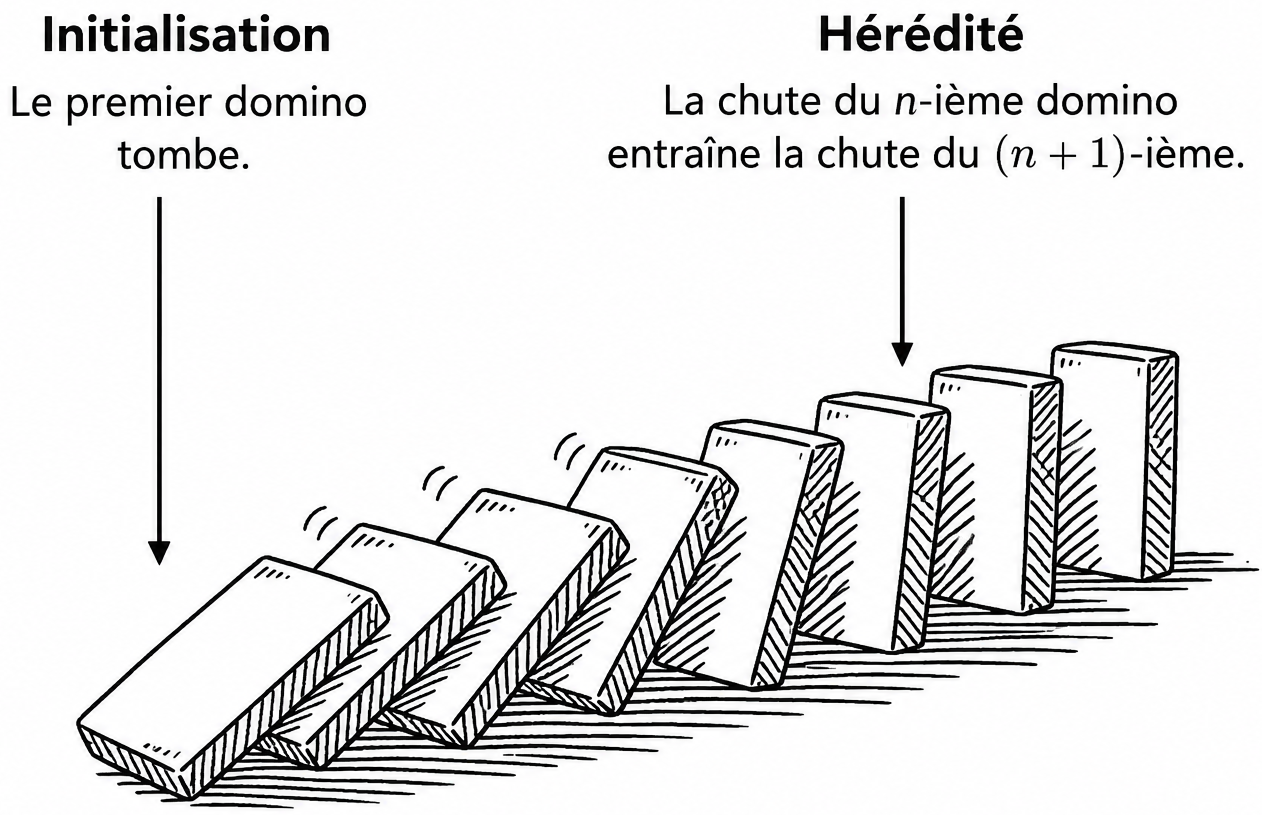
\includegraphics[width=\linewidth]{figures/analyse/domino}	
\end{minipage}
\subsection{Principe du raisonnement par récurrence}
\begin{theoreme}[Principe de récurrence]
	
Soit $P(n)$ une propriété qui dépend d'un nombre naturel $n$ et
$n_0$ un entier naturel fixé.

Si la propriété $P(n)$ vérifie les deux conditions suivantes :

\begin{enumerate}
	\item \textbf{Initialisation :} $P(n_0)$ est vraie ;
	
	\item \textbf{Hérédité :} si $P(k)$ est vraie pour un entier naturel
	$k \geq n_0$, alors $P(k+1)$ est vraie
\end{enumerate}

alors, \textbf{pour tout entier naturel $n \geq n_0$},
$P(n)$ est vraie.
\end{theoreme}

\remarque 
\begin{itemize}
	
	\item La propriété $P(n)$ peut être une égalité, une inégalité, une propriété exprimée par une phrase, \ldots
	
	\item La condition d'hérédité est une implication : on suppose que
	$P(k)$ est vraie pour un nombre entier naturel $k$ supérieur ou égal à
	$n_0$ (c'est \textbf{l'hypothèse de récurrence}) et on montre qu'alors
	$P(k+1)$ est vraie elle aussi.
	
	Une propriété $P(n)$ qui vérifie cette deuxième condition est dite
	héréditaire à partir du rang $n_0$ ; en effet, elle se transmet du nombre entier
	$k$ à son « successeur » $k+1$.
	
\end{itemize}

\begin{center}
	
\includegraphics[width=\textwidth]{analyse/resume_recurrence}
\end{center}

\exerciceresolu 
$(u_n)$ est la suite définie par $u_0=0$ et pour tout entier naturel $n, u_{n+1}=2u_n+1 $

Démontrer par récurrence que, pour tout entier naturel $u_n=2^n-1.$

\solution
\begin{itemize}[label=\textbullet]
	
	\item \textbf{Initialisation :} Pour $n=0$, $u_0=0$ et $2^0-1=0$. Ainsi $P(0)$ est vraie.
	
	\item \textbf{Hérédité :} Supposons $P(k)$ vraie, c'est-à-dire $u_k=2^k-1$ (hypothèse de récurrence).\\
	Démontrons qu'alors que $P(k+1)$ est vraie, c'est-à-dire que $u_{k+1}=2^{k+1}-1.$ \\
	Or, $u_{k+1}=2u_k+1$. Ainsi, d'après l'hypothèse de récurrence,
	$u_{k+1}=2(2^k-1)+1=2^{k+1}-1$.
	
	Alors
	$$
	u_{k+1}=2u_k+1
	=2(2^k-1)+1
	=2^{k+1}-1.
	$$
	
	Donc $P(k+1)$ est vraie.
	
	\item \textbf{Conclusion :} La propriété est vraie pour tout entier naturel $n$.
	
\end{itemize}


Sur le modèle de l'exercice résolu ci-dessus :
\exercice{\etoilepleine\etoilevide\etoilevide}
\begin{minipage}[t]{0.46\textwidth}
	
	\textbf{1)} $(v_n)$ est la suite définie par $v_0=0$ et
	$v_{n+1}=v_n+2n+2$.
	
	Démontrer par récurrence que, pour tout entier naturel $n$,
	$v_n=n(n+1)$.
	
\end{minipage}
\hfill
\vrule width 1pt
\hfill
\begin{minipage}[t]{0.46\textwidth}
	\textbf{2)} $(w_n)$ est la suite définie par $w_0=0$ et
	$w_{n+1}=2w_n-3$.
	
	Démontrer par récurrence que, pour tout entier naturel $n$,
	$w_n=3(1-2^n)$.
	
\end{minipage}






	% ============================================================
%  CHAPITRE : ÉQUATIONS DIFFÉRENTIELLES
%  Mazava Maths — Terminale S (Bacc Série S, Madagascar)
%  Aligné sur le modèle type et le programme officiel MESUPRES
%  (y'=ky, y'+ay=0, y'+ay=b ; ay''+by'+cy=0 : équation
%  caractéristique, 3 cas ; y''=m^2 y, y''=-m^2 y ; conditions
%  initiales ; vérifier qu'une fonction est solution ; second
%  membre : solution particulière + homogène).
%  Environnements : definition, propriete, theoreme, methode,
%                   attention, astucebac, exemple, exercice,
%                   solution, remarque
% ============================================================

\chapter{Équations différentielles}

\begin{citationchapitre}
	« Les lois de la nature ne sont rien d'autre que des relations entre une
	grandeur et ses variations. »\\[0.4em]
	— adage de physique mathématique
\end{citationchapitre}

\begin{objectifs}
	\begin{itemize}[label=\textbullet]
		\item Reconnaître une équation différentielle et son \textbf{ordre}.
		\item Résoudre $y'=ky$, $y'+ay=0$, $y'+ay=b$ ($a$, $b$ constants).
		\item \textbf{Vérifier} qu'une fonction donnée est solution.
		\item Résoudre $ay''+by'+cy=0$ par l'\textbf{équation caractéristique}
		(trois cas) ; cas $y''=m^{2}y$ et $y''=-m^{2}y$.
		\item Déterminer la solution vérifiant des \textbf{conditions initiales}
		(problème de Cauchy).
		\item Traiter une équation \textbf{avec second membre} : solution
		particulière $+$ solution générale de l'équation homogène.
	\end{itemize}
\end{objectifs}


% ================================================================
\section{Généralités}
% ================================================================

\begin{definition}
	Une \textbf{équation différentielle} est une équation dont l'inconnue est
	une \textbf{fonction} $y$ et qui fait intervenir $y$ et ses dérivées
	($y'$, $y''$,\ldots). Son \textbf{ordre} est l'ordre de dérivation le plus
	élevé qui y figure. \textbf{Résoudre} (ou \textbf{intégrer}) l'équation
	sur $I$, c'est en déterminer \emph{toutes} les fonctions solutions sur $I$.
\end{definition}

\begin{methode}
	\textbf{Vérifier qu'une fonction $\varphi$ est solution de $(E)$ :}
	\begin{enumerate}
		\item calculer $\varphi'$ (et $\varphi''$ si besoin) ;
		\item reporter dans le \textbf{premier membre} de $(E)$ ;
		\item simplifier et vérifier l'égalité avec le second membre.
	\end{enumerate}
\end{methode}

\begin{exemple}
	La fonction $\varphi(x)=\e^{-2x}+3$ est-elle solution de $y'+2y=6$ ?

	$\varphi'(x)=-2\e^{-2x}$, donc
	$\varphi'+2\varphi=-2\e^{-2x}+2\e^{-2x}+6=6$. \ Oui, $\varphi$ est solution.
\end{exemple}


% ================================================================
\section{Équations différentielles du premier ordre}
% ================================================================

\begin{theoreme}[Équation homogène $y'+ay=0$]
	Soit $a\in\R$. Les solutions sur $\R$ de $\;y'+ay=0\;$ (c'est-à-dire
	$y'=-ay$) sont les fonctions
	\[
	x\longmapsto C\,\e^{-ax},\qquad C\in\R.
	\]
	En particulier, les solutions de $y'=ky$ sont $x\mapsto C\,\e^{kx}$.
\end{theoreme}

\begin{center}
\begin{tikzpicture}[>=Stealth, scale=1.0]
	\begin{scope}
		\clip (-2.3,-2.5) rectangle (3.4,2.6);
		\foreach \c in {-2,-1,1,2}
			\draw[gray!55,thick] plot[domain=-2.3:3.4,samples=90]
			  (\x,{\c*exp(-\x)});
		\draw[very thick,black] plot[domain=-2.3:3.4,samples=110]
		  (\x,{exp(1-\x)});
	\end{scope}
	\draw[->] (-2.5,0) -- (3.7,0) node[right,font=\small] {$x$};
	\draw[->] (0,-2.7) -- (0,2.9) node[above,font=\small] {$y$};
	\draw[gray!60,dashed] (1,0) node[below,font=\scriptsize] {$x_0$}
	  -- (1,1) -- (0,1) node[left,font=\scriptsize] {$y_0$};
	\filldraw (1,1) circle (1.6pt) node[above right,font=\scriptsize] {$A$};
	\node[font=\scriptsize,align=center] at (2.5,1.9)
	  {solution telle que\\ $y(x_0)=y_0$};
	\node[font=\scriptsize,gray] at (-1.7,-1.9) {$y=C\,\e^{-ax}$};
\end{tikzpicture}
\end{center}

\begin{remarque}
	L'équation $y'+ay=0$ a une \textbf{infinité} de solutions : une par valeur
	de $C$ (le \textbf{faisceau} de courbes ci-dessus). Une \textbf{condition
	initiale} $y(x_0)=y_0$ en sélectionne \textbf{une seule}.
\end{remarque}

\begin{theoreme}[Équation complète $y'+ay=b$]
	Soient $a\neq 0$ et $b$ deux réels. Les solutions sur $\R$ de $\;y'+ay=b\;$
	sont les fonctions
	\[
	x\longmapsto C\,\e^{-ax}+\frac{b}{a},\qquad C\in\R.
	\]
\end{theoreme}

\begin{remarque}
	La solution générale de $y'+ay=b$ est la somme de la solution générale de
	l'équation homogène $y'+ay=0$ et d'une \textbf{solution particulière
	constante} $y_0=\dfrac{b}{a}$.
\end{remarque}

\begin{propriete}{Unicité sous condition initiale}{prop_cauchy_1}
	Pour tout $(x_0\,;y_0)$, il existe une \textbf{unique} solution $f$ de
	$y'+ay=b$ vérifiant $f(x_0)=y_0$.
\end{propriete}

\begin{methode}
	\textbf{Problème de Cauchy} $\bigl(y'+ay=b,\ y(x_0)=y_0\bigr)$ :
	\begin{enumerate}
		\item écrire la solution générale $y(x)=C\e^{-ax}+\dfrac{b}{a}$ ;
		\item imposer $y(x_0)=y_0$, résoudre en $C$ ;
		\item conclure.
	\end{enumerate}
\end{methode}

\exerciceresolu
Résoudre $(E):2y'+3y=6$, puis trouver la solution $f$ telle que $f(0)=-1$.

\solution

On divise par $2$ : $y'+\dfrac32 y=3$, donc $a=\dfrac32$, $b=3$.
Solution générale :
\[
y(x)=C\,\e^{-\frac32 x}+\frac{3}{\frac32}=C\,\e^{-\frac32 x}+2,\qquad C\in\R.
\]
Condition : $f(0)=C+2=-1$, d'où $C=-3$ :
\[
\boxed{f(x)=-3\,\e^{-\frac32 x}+2.}
\]


% ================================================================
\section{Équations du second ordre \texorpdfstring{$ay''+by'+cy=0$}{ay''+by'+cy=0}}
% ================================================================

\begin{definition}
	Soient $a$, $b$, $c$ réels avec $a\neq 0$. L'\textbf{équation
	caractéristique} de $(E):ay''+by'+cy=0$ est l'équation du second degré
	\[
	(E_c):\quad a r^{2}+b r+c=0\qquad (r\in\C).
	\]
\end{definition}

\begin{theoreme}[Résolution selon le discriminant]
	Soit $\Delta=b^{2}-4ac$ le discriminant de $(E_c)$. Les solutions sur $\R$
	de $ay''+by'+cy=0$ sont :
	\begin{center}
	\renewcommand{\arraystretch}{2.0}
	\begin{tabular}{>{\raggedright\arraybackslash}p{3.4cm}
	                >{\raggedright\arraybackslash}p{5.0cm}}
	\hline
	$\Delta>0$ : deux racines réelles $r_1\neq r_2$
	& $y(x)=A\,\e^{r_1 x}+B\,\e^{r_2 x}$ \\
	$\Delta=0$ : racine double $r_0=-\dfrac{b}{2a}$
	& $y(x)=(Ax+B)\,\e^{r_0 x}$ \\
	$\Delta<0$ : racines $\alpha\pm\ii\beta$ ($\beta\neq 0$)
	& $y(x)=\e^{\alpha x}\bigl(A\cos\beta x+B\sin\beta x\bigr)$ \\
	\hline
	\end{tabular}
	\end{center}
	($A$, $B$ décrivent $\R$.)
\end{theoreme}

\begin{attention}
	Dans le cas $\Delta<0$, ne pas confondre le coefficient $\alpha$ de
	l'exponentielle (partie réelle de $r$) et la pulsation $\beta$ dans
	$\cos\beta x$, $\sin\beta x$ (partie imaginaire).
\end{attention}

\begin{propriete}{Cas particuliers du programme}{prop_cas_part}
	Soit $m>0$.
	\begin{itemize}[label=\textbullet]
		\item $y''=m^{2}y$ \ ($y''-m^{2}y=0$) : \
		$y(x)=A\,\e^{mx}+B\,\e^{-mx}$.
		\item $y''=-m^{2}y$ \ ($y''+m^{2}y=0$) : \
		$y(x)=A\cos(mx)+B\sin(mx)$.
	\end{itemize}
\end{propriete}

\begin{astucebac}
	Problème de Cauchy au second ordre : on donne \textbf{deux} conditions
	(souvent $y(0)$ et $y'(0)$). Calculer proprement $y'(x)$ en fonction de
	$A$, $B$ \textbf{avant} de substituer.
\end{astucebac}

\exerciceresolu
Résoudre $(E):y''-4y'+13y=0$ avec $y(0)=2$ et $y'(0)=7$.

\solution

$(E_c):r^{2}-4r+13=0$, $\Delta=16-52=-36<0$ : racines
$r=\dfrac{4\pm 6\ii}{2}=2\pm 3\ii$, donc $\alpha=2$, $\beta=3$.
\[
y(x)=\e^{2x}\bigl(A\cos 3x+B\sin 3x\bigr).
\]
$y'(x)=2\e^{2x}\bigl(A\cos 3x+B\sin 3x\bigr)
+\e^{2x}\bigl(-3A\sin 3x+3B\cos 3x\bigr)$.
\[
y(0)=A=2,\qquad y'(0)=2A+3B=7\ \Rightarrow\ 4+3B=7\ \Rightarrow\ B=1.
\]
\[
\boxed{f(x)=\e^{2x}\bigl(2\cos 3x+\sin 3x\bigr).}
\]


% ================================================================
\section{Équations avec second membre}
% ================================================================

\begin{theoreme}[Structure des solutions]
	Soit $(E)$ une équation différentielle linéaire (ordre $1$ ou $2$) et
	$(E_0)$ l'équation \textbf{homogène} associée (sans second membre).
	Si $y_p$ est \textbf{une} solution particulière de $(E)$, alors
	\[
	f \text{ solution de } (E)
	\iff f-y_p \text{ solution de } (E_0).
	\]
	Donc : \ \textbf{solution générale de $(E)$} $=$ \textbf{solution
	particulière} $+$ \textbf{solution générale de $(E_0)$}.
\end{theoreme}

\begin{methode}
	Pour résoudre $(E)$ avec second membre (sujet guidé) :
	\begin{enumerate}
		\item résoudre l'équation homogène $(E_0)$ ;
		\item déterminer une solution particulière $y_p$ (forme donnée dans
		l'énoncé : on identifie les coefficients) ;
		\item la solution générale de $(E)$ est $y_p+$ (solution générale de $(E_0)$) ;
		\item appliquer les conditions initiales.
	\end{enumerate}
\end{methode}

\exerciceresolu
$(E):y'+2y=(4x+2)\,\e^{-2x}$.
\begin{enumerate}
	\item Résoudre $(E_0):y'+2y=0$.
	\item Déterminer $a$, $b$ tels que $y_p(x)=(a x^{2}+bx)\,\e^{-2x}$ soit
	solution de $(E)$.
	\item En déduire la solution générale de $(E)$, puis la solution $h$
	telle que $h(0)=1$.
\end{enumerate}

\solution

\textbf{1.} $(E_0)$ : $y(x)=C\,\e^{-2x}$, $C\in\R$.

\textbf{2.} $y_p(x)=(a x^{2}+bx)\e^{-2x}$, donc
$y_p'(x)=\bigl[(2ax+b)-2(a x^{2}+bx)\bigr]\e^{-2x}$, et
\[
y_p'+2y_p=(2a x+b)\,\e^{-2x}.
\]
On veut $2a x+b=4x+2$, d'où $a=2$ et $b=2$ :
$y_p(x)=(2x^{2}+2x)\e^{-2x}$.

\textbf{3.} Solution générale : $y(x)=\bigl(2x^{2}+2x+C\bigr)\e^{-2x}$.
$h(0)=C=1$, donc $h(x)=(2x^{2}+2x+1)\,\e^{-2x}$.


% ================================================================
\section{Exercices d'entraînement}
% ================================================================

% --------------------------------------------------
\subsection{Échauffement}
% --------------------------------------------------

\exercice{Lire un faisceau de courbes \hfill \facile}
La figure ci-dessous représente quatre solutions de l'équation
différentielle $(E):y'+y=0$.

\begin{center}
\begin{tikzpicture}[>=Stealth, scale=0.95]
	\begin{scope}
		\clip (-2.7,-2.6) rectangle (2.9,2.6);
		\draw[thick,domain=-1.4:2.7,samples=110] plot (\x,{exp(-\x)});
		\draw[thick,domain=-0.35:2.7,samples=110] plot (\x,{3*exp(-\x)});
		\draw[thick,domain=-2.7:1.4,samples=110] plot (\x,{-exp(-\x)});
	\end{scope}
	\draw[->] (-2.9,0) -- (3.1,0) node[right,font=\small] {$x$};
	\draw[->] (0,-2.8) -- (0,2.9) node[above,font=\small] {$y$};
	\node[font=\scriptsize] at (2.35,0.7) {$C=1$};
	\node[font=\scriptsize] at (1.35,1.55) {$C=3$};
	\node[font=\scriptsize] at (1.9,-0.85) {$C=-1$};
	\node[font=\scriptsize,gray] at (-2.0,0.3) {$C=0$};
\end{tikzpicture}
\end{center}

\begin{enumerate}
	\item Donner la forme générale des solutions de $(E)$.
	\item Identifier la solution qui vérifie $y(0)=3$.
	\item Combien de solutions vérifient $y(0)=0$ ?
	\item Quelle est la limite commune de toutes les solutions en $+\infty$ ?
\end{enumerate}

\exercice{Un faisceau avec second membre \hfill \facile}
La figure ci-dessous représente quatre solutions de l'équation
différentielle $(E):y'+y=2$.

\begin{center}
\begin{tikzpicture}[>=Stealth, scale=0.9]
	\begin{scope}
		\clip (-2.4,-2.4) rectangle (3.4,4.2);
		\foreach \c in {-2,-1,1}
			\draw[thick,domain=-2.4:3.4,samples=110]
			  plot (\x,{2+\c*exp(-\x)});
		\draw[thick,domain=-2.4:3.4,samples=110] plot (\x,{2+2.7*exp(-\x)});
	\end{scope}
	\draw[->] (-2.6,0) -- (3.7,0) node[right,font=\small] {$x$};
	\draw[->] (0,-2.5) -- (0,4.4) node[above,font=\small] {$y$};
	\draw[red!70!black,dashed] (-2.4,2) -- (3.5,2)
	  node[right,font=\scriptsize,red!70!black] {$y=2$};
	\node[font=\scriptsize] at (2.7,2.5) {solutions};
\end{tikzpicture}
\end{center}

\begin{enumerate}
	\item Donner la forme générale des solutions de $(E)$.
	\item Quelle est la limite commune de toutes les solutions en $+\infty$ ?
	Interpréter la droite $y=2$.
	\item Identifier la solution constante.
	\item Déterminer la solution vérifiant $y(0)=0$.
\end{enumerate}

\exercice{Vrai ou faux \hfill \facile}
Répondre par \emph{vrai} ou \emph{faux} en justifiant.
\begin{enumerate}
	\item L'équation $y'=3y$ a pour solutions $x\mapsto C\,\e^{3x}$.
	\item $x\mapsto \e^{2x}$ est solution de $y''-4y=0$.
	\item Les solutions de $y''+4y=0$ sont périodiques.
	\item Une équation différentielle a toujours une infinité de solutions.
	\item Si $y_p$ est une solution de $(E):y'+ay=b$, alors $2y_p$ aussi.
	\item Pour $y''=-9y$, la pulsation des solutions est $9$.
	\item La solution de $y'+2y=0$ avec $y(0)=0$ est la fonction nulle.
\end{enumerate}

% --------------------------------------------------
\subsection{Premier ordre}
% --------------------------------------------------

\exercice{Solution générale \hfill \facile}
Résoudre sur $\R$ (solution générale).
\begin{multicols}{2}
\begin{enumerate}
	\item $y'-7y=0$
	\item $2y'+5y=0$
	\item $y'=-3y$
	\item $y'+3y=6$
	\item $4y'-y=5$
	\item $3y'+2y=0$
\end{enumerate}
\end{multicols}

\exercice{Problème de Cauchy \hfill \moyen}
Déterminer la solution vérifiant la condition indiquée.
\begin{multicols}{2}
\begin{enumerate}
	\item $y'=-2y$, \ $y(0)=3$
	\item $y'-4y=12$, \ $y(0)=-1$
	\item $3y'+2y=4$, \ $y(3)=2$
	\item $y'+y=1$, \ $y(0)=0$
\end{enumerate}
\end{multicols}

\exercice{Décroissance radioactive \hfill \moyen}
La masse $m(t)$ (en g) d'un échantillon radioactif vérifie
$m'(t)=-\lambda\,m(t)$ avec $\lambda>0$, et $m(0)=m_0$.
\begin{enumerate}
	\item Exprimer $m(t)$.
	\item La \emph{demi-vie} $T$ est le temps au bout duquel la masse est
	divisée par $2$. Montrer que $T=\dfrac{\ln 2}{\lambda}$.
	\item Déterminer $\displaystyle\lim_{t\to+\infty}m(t)$.
\end{enumerate}

% --------------------------------------------------
\subsection{Second ordre}
% --------------------------------------------------

\exercice{Équation caractéristique \hfill \moyen}
Résoudre sur $\R$ (solution générale).
\begin{multicols}{2}
\begin{enumerate}
	\item $y''-5y'+6y=0$
	\item $y''+6y'+9y=0$
	\item $y''-2y'+5y=0$
	\item $y''-y=0$
	\item $y''+4y=0$
	\item $y''+2y'+2y=0$
\end{enumerate}
\end{multicols}

\exercice{Cauchy au second ordre \hfill \moyen}
\begin{enumerate}
	\item $y''-3y'+2y=0$, \ $y(0)=4$, \ $y'(0)=0$.
	\item $y''+9y=0$, \ $y(0)=1$, \ $y'\!\left(\dfrac{\pi}{6}\right)=0$.
	Montrer que $f(x)$ s'écrit $A\cos(3x+\varphi)$.
\end{enumerate}

\exercice{Oscillations à Analakely \hfill \moyen}
Un système mécanique oscillant est régi par $(E):y''+16y=0$.
\begin{enumerate}
	\item Donner la forme générale des solutions de $(E)$.
	\item Déterminer la solution $g$ telle que
	$g(0)=\dfrac{\sqrt3}{2}$ et $g'(0)=2$.
	\item Vérifier que $g(t)=\cos\!\left(4t-\dfrac{\pi}{6}\right)$ pour tout
	réel $t$.
\end{enumerate}

% --------------------------------------------------
\subsection{Sujets types Bac}
% --------------------------------------------------

\exercice{Sujet type Bac — équation avec second membre \hfill \difficile}
On considère $(E):y'+2y=(3x+1)\,\e^{-2x}$.

\textbf{Partie A}
\begin{enumerate}
	\item Résoudre $(E_0):y'+2y=0$ sur $\R$.
	\item Déterminer $a$, $b$ tels que $u(x)=(a x^{2}+bx)\,\e^{-2x}$ soit
	solution de $(E)$.
	\item Démontrer que $f$ est solution de $(E)$ si et seulement si $f-u$ est
	solution de $(E_0)$.
	\item En déduire l'ensemble des solutions de $(E)$, puis la solution $h$
	telle que $h(0)=2$.
\end{enumerate}

\textbf{Partie B — Modèle thermique}
La température $T(t)$ (en $^{\circ}$C) d'un composant après $t$ minutes est
\[
T(t)=\left(\frac32 t^{2}+t+25\right)\e^{-2t}+20\qquad (t\geq 0).
\]
\begin{enumerate}
	\setcounter{enumi}{4}
	\item Donner la température initiale.
	\item Déterminer $\displaystyle\lim_{t\to+\infty}T(t)$ et l'interpréter.
	\item Calculer $T'(t)$ et étudier son signe sur $[0\,;+\infty[$.
	\item À quel instant $T$ est-elle maximale ? Donner cette température à
	$0{,}1\,^{\circ}$C près.
\end{enumerate}

\exercice{Sujet type Bac — vérifier une solution, puis résoudre \hfill \difficile}
On considère $(E):y'-2y=\dfrac{-2}{1+\e^{-2x}}$ et la fonction
$g(x)=\e^{2x}\ln\!\bigl(1+\e^{-2x}\bigr)$.

\textbf{Partie A}
\begin{enumerate}
	\item Calculer $g'(x)$ et vérifier que $g$ est solution de $(E)$.
	\item Résoudre l'équation homogène $(E_0):y'-2y=0$.
	\item Montrer que $f$ est solution de $(E)$ si et seulement si $f-g$ est
	solution de $(E_0)$.
	\item En déduire la solution générale de $(E)$.
\end{enumerate}

\textbf{Partie B}
\begin{enumerate}
	\setcounter{enumi}{4}
	\item Déterminer $\displaystyle\lim_{x\to-\infty}g(x)$ et
	$\displaystyle\lim_{x\to+\infty}g(x)$ (poser $X=\e^{-2x}$).
	\item En déduire une asymptote à $\mathcal C_g$.
\end{enumerate}

\exercice{Sujet type Bac — tangente imposée \hfill \difficile}
On considère $(E):y''-3y'+2y=0$.
\begin{enumerate}
	\item Résoudre $(E)$ sur $\R$.
	\item Déterminer la solution $f$ dont la courbe passe par $A(0\,;4)$ et
	admet en $A$ une tangente parallèle à l'axe des abscisses.
	\item Étudier les variations de $f$ sur $\R$ et déterminer
	$\displaystyle\lim_{x\to-\infty}f(x)$, $\displaystyle\lim_{x\to+\infty}f(x)$.
	\item Étudier la convexité de $f$ ; montrer que $\mathcal C_f$ a un point
	d'inflexion.
\end{enumerate}

\exercice{Sujet type Bac — pendule et énergie \hfill \difficile}
Pour de petites oscillations, l'angle $\theta(t)$ d'un pendule vérifie
$(E):\theta''+\omega^{2}\theta=0$ ($\omega>0$).
\begin{enumerate}
	\item Donner la solution générale de $(E)$.
	\item À $t=0$, le pendule est écarté de $\theta_0$ et lâché sans vitesse.
	Déterminer $\theta(t)$.
	\item Montrer que l'accélération $\theta''(t)$ est proportionnelle à
	$\theta(t)$ ; préciser le coefficient.
	\item On pose $E(t)=\bigl(\theta'(t)\bigr)^{2}+\omega^{2}\bigl(\theta(t)\bigr)^{2}$.
	Montrer que $E$ est \textbf{constante}.
\end{enumerate}

\exercice{Sujet type Bac — équation avec second membre trigonométrique \hfill \difficile}
On considère $(E):y''+y=\cos x$.
\begin{enumerate}
	\item Résoudre l'équation homogène $(E_0):y''+y=0$.
	\item Montrer que $u(x)=\dfrac12\,x\sin x$ est une solution particulière
	de $(E)$.
	\item En déduire la solution générale de $(E)$.
	\item Déterminer la solution $f$ telle que $f(0)=0$ et $f'(0)=0$.
	\item Calculer $\displaystyle\int_0^{\pi}f(x)\dd x$.
\end{enumerate}

\exercice{Sujet type Bac — changement d'inconnue \hfill \difficile}
On résout sur $I=]0\,;+\infty[$ l'équation $(E):x^{2}y''+3xy'+y=0$.
On pose $z(t)=y(\e^{t})$ pour tout réel $t$.
\begin{enumerate}
	\item Exprimer $z'(t)$ et $z''(t)$ en fonction de $y'(\e^{t})$,
	$y''(\e^{t})$ et $\e^{t}$.
	\item Montrer que $y$ est solution de $(E)$ sur $I$ si et seulement si $z$
	est solution d'une équation $(E'):z''+2z'+z=0$.
	\item Résoudre $(E')$ sur $\R$.
	\item En déduire les solutions de $(E)$ sur $I$.
\end{enumerate}

	
%	\part{Géométrie}
	
	% ============================================================
%   CHAPITRE : Barycentre
%   Niveau   : Terminale S / Terminale C
%   Mazava Maths
% ============================================================
\chapter{Barycentre}
\begin{citationchapitre}
	« La géométrie est la science du raisonnement correct\\
	sur des figures incorrectement dessinées. »\\[0.4em]
	— Henri Poincaré
\end{citationchapitre}

\begin{objectifs}
	\begin{itemize}[label=\textbullet]
		\item Définir et construire le barycentre d'un système de points pondérés.
		\item Utiliser les propriétés d'associativité et de linéarité du barycentre.
		\item Déterminer et construire les lignes de niveau (ensembles de points).
		\item Appliquer le barycentre en géométrie analytique et aux centres remarquables.
	\end{itemize}
\end{objectifs}


% ============================================================
\section{Définition et existence du barycentre}
% ============================================================

\begin{definition}
	Soient $A_1, A_2, \ldots, A_n$ des points du plan et $\alpha_1, \alpha_2, \ldots, \alpha_n$
	des réels tels que $\alpha_1 + \alpha_2 + \cdots + \alpha_n \neq 0$.
	
	Il existe un unique point $G$ vérifiant :
	$$
	\alpha_1\,\vect{GA_1} + \alpha_2\,\vect{GA_2} + \cdots + \alpha_n\,\vect{GA_n} = \vect{0}.
	$$
	Ce point $G$ s'appelle le \textbf{barycentre} du système de points pondérés
	$$
	\{(A_1,\alpha_1)\,;\,(A_2,\alpha_2)\,;\,\ldots\,;\,(A_n,\alpha_n)\}.
	$$
	
	Les réels $\alpha_i$ s'appellent les \textbf{coefficients} (ou \textbf{poids}) du système.
\end{definition}

\begin{attention}
	Le barycentre n'existe que si la somme des coefficients est \textbf{non nulle}.
	Si $\alpha_1 + \alpha_2 + \cdots + \alpha_n = 0$, le système n'admet pas de barycentre.
\end{attention}

\begin{propriete}{Caractérisation vectorielle}{}
	$G$ est le barycentre de $\{(A_i, \alpha_i)\}$ si et seulement si pour tout point $M$
	du plan :
	$$
	\sum_{i=1}^{n} \alpha_i\,\vect{MA_i} = \left(\sum_{i=1}^{n} \alpha_i\right)\vect{MG}.
	$$
\end{propriete}

\begin{exemple}
	Soient $A$, $B$ deux points et $\alpha, \beta$ deux réels avec $\alpha + \beta \neq 0$.
	
	Le barycentre $G$ de $\{(A,\alpha)\,;\,(B,\beta)\}$ vérifie :
	$$
	\alpha\,\vect{GA} + \beta\,\vect{GB} = \vect{0}
	\iff \vect{AG} = \frac{\beta}{\alpha+\beta}\,\vect{AB}.
	$$
	$G$ divise $[AB]$ dans le rapport $\dfrac{\beta}{\alpha}$ à partir de $A$.
\end{exemple}

\begin{propriete}{Cas de deux points}{}
	Le barycentre $G$ de $\{(A,\alpha)\,;\,(B,\beta)\}$ avec $\alpha + \beta \neq 0$
	vérifie :
	$$
	\vect{AG} = \frac{\beta}{\alpha+\beta}\,\vect{AB}.
	$$
	\begin{itemize}[label=\textbullet]
		\item Si $\alpha = \beta$ : $G$ est le \textbf{milieu} de $[AB]$.
		\item Si $\alpha + \beta > 0$ et $\alpha, \beta > 0$ : $G$ est entre $A$ et $B$.
		\item Si les coefficients sont de signes opposés : $G$ est à l'extérieur de $[AB]$.
	\end{itemize}
\end{propriete}


% ============================================================
\section{Propriétés fondamentales}
% ============================================================

\begin{propriete}{Associativité du barycentre}{}
	Soient $G_1$ le barycentre de $\{(A_i, \alpha_i)_{i \in I}\}$ et
	$G_2$ le barycentre de $\{(A_j, \alpha_j)_{j \in J}\}$, avec $I \cap J = \emptyset$.
	
	Alors le barycentre de l'ensemble $\{(A_i, \alpha_i)_{i \in I \cup J}\}$
	est aussi le barycentre de
	$$
	\left\{\left(G_1,\ \sum_{i \in I}\alpha_i\right)\,;\,\left(G_2,\ \sum_{j \in J}\alpha_j\right)\right\}.
	$$
\end{propriete}

\remarque
Cette propriété permet de calculer un barycentre \textbf{en plusieurs étapes},
en regroupant d'abord certains points entre eux.

\begin{exemple}
	Calculer le barycentre $G$ de $\{(A,1)\,;\,(B,2)\,;\,(C,3)\}$.
	
	\textbf{Étape 1 :} On calcule $G_1 = $ barycentre de $\{(A,1)\,;\,(B,2)\}$
	avec poids total $3$.
	
	\textbf{Étape 2 :} Par associativité, $G = $ barycentre de $\{(G_1, 3)\,;\,(C,3)\}$,
	donc $G$ est le \textbf{milieu} de $[G_1C]$.
\end{exemple}

\begin{propriete}{Linéarité — relation de Chasles généralisée}{}
	Pour tout point $M$ du plan et tout système $\{(A_i, \alpha_i)\}$ de somme
	$\sigma = \sum \alpha_i \neq 0$ de barycentre $G$ :
	$$
	\sum_{i=1}^{n} \alpha_i\,\vect{MA_i} = \sigma\,\vect{MG}.
	$$
	En particulier, pour tout vecteur $\vec{u}$ :
	$$
	\sum_{i=1}^{n} \alpha_i\,\overrightarrow{A_i} = \sigma\,\overrightarrow{G},
	$$
	où les vecteurs positions sont pris depuis une même origine.
\end{propriete}

\begin{propriete}{Coordonnées du barycentre}{}
	Dans un repère, si $A_i$ a pour coordonnées $(x_i, y_i)$, alors le barycentre
	$G$ de $\{(A_i, \alpha_i)\}$ a pour coordonnées :
	$$
	x_G = \frac{\sum \alpha_i x_i}{\sum \alpha_i},
	\qquad
	y_G = \frac{\sum \alpha_i y_i}{\sum \alpha_i}.
	$$
\end{propriete}

\begin{exemple}
	Soient $A(1\,;\,2)$, $B(3\,;\,0)$, $C(-1\,;\,4)$ avec coefficients $2$, $1$, $3$.
	
	$$
	x_G = \frac{2 \times 1 + 1 \times 3 + 3 \times (-1)}{2+1+3}
	= \frac{2 + 3 - 3}{6} = \frac{2}{6} = \frac{1}{3}.
	$$
	$$
	y_G = \frac{2 \times 2 + 1 \times 0 + 3 \times 4}{6}
	= \frac{4 + 0 + 12}{6} = \frac{16}{6} = \frac{8}{3}.
	$$
	
	Donc $G\!\left(\dfrac{1}{3}\,;\,\dfrac{8}{3}\right)$.
\end{exemple}


% ============================================================
\section{Centres remarquables d'un triangle}
% ============================================================

\begin{propriete}{Centres remarquables comme barycentres}{}
	Soit $ABC$ un triangle.
	\begin{enumerate}
		\item Le \textbf{centre de gravité} $G$ est le barycentre de
		$\{(A,1)\,;\,(B,1)\,;\,(C,1)\}$. Il vérifie $\vect{GA} + \vect{GB} + \vect{GC} = \vect{0}$.

		\item L'\textbf{orthocentre} $H$ est le barycentre de
		$$
		\{(A,\tan\hat{A})\,;\,(B,\tan\hat{B})\,;\,(C,\tan\hat{C})\}.
		$$
		
		\item Le \textbf{centre du cercle circonscrit} $O$ est le barycentre de
		$$
		\{(A,\sin 2\hat{A})\,;\,(B,\sin 2\hat{B})\,;\,(C,\sin 2\hat{C})\}.
		$$
	\end{enumerate}
\end{propriete}

\begin{propriete}{Relation d'Euler}{}
	Dans tout triangle $ABC$, en notant $G$ le centre de gravité,
	$H$ l'orthocentre et $O$ le centre du cercle circonscrit :
	$$
	\vect{OH} = 3\,\vect{OG}.
	$$
	Les points $O$, $G$, $H$ sont \textbf{alignés} (droite d'Euler) et $OG = \dfrac{1}{3}OH$.
\end{propriete}


% ============================================================
\section{Lignes de niveau}
% ============================================================

\begin{definition}
	\textbf{Ligne de niveau}\par
	Soit $\{(A_i, \alpha_i)\}$ un système de points pondérés de barycentre $G$.
	Pour tout réel $k$, l'\textbf{ensemble de niveau $k$} est :
	$$
	\mathscr{E}_k = \left\{ M \in \mathscr{P} \;\middle|\;
	\sum_{i=1}^{n} \alpha_i\,MA_i^2 = k \right\}.
	$$
\end{definition}

\begin{theoreme}
	\textbf{Réduction de la somme pondérée des carrés}\par
	Soit $G$ le barycentre de $\{(A_i, \alpha_i)\}$ de somme $\sigma = \sum \alpha_i \neq 0$.
	Pour tout point $M$ :
	$$
	\sum_{i=1}^{n} \alpha_i\,MA_i^2
	= \sigma\,MG^2 + \sum_{i=1}^{n} \alpha_i\,GA_i^2.
	$$
\end{theoreme}

\remarque
On pose $\displaystyle K = \sum_{i=1}^{n} \alpha_i\,GA_i^2$ (constante indépendante de $M$).
La formule devient :
$$
\sum_{i=1}^{n} \alpha_i\,MA_i^2 = \sigma\,MG^2 + K.
$$

\begin{propriete}{Nature des lignes de niveau}{}
	Avec les notations ci-dessus :
	
	\begin{enumerate}
		\item \textbf{Si $\sigma > 0$} : l'ensemble $\mathscr{E}_k$ est
		\begin{itemize}[label=\textbullet]
			\item un \textbf{cercle} de centre $G$ et de rayon $r = \sqrt{\dfrac{k-K}{\sigma}}$
			si $k > K$,
			\item le \textbf{point} $G$ si $k = K$,
			\item l'\textbf{ensemble vide} si $k < K$.
		\end{itemize}
		
		\item \textbf{Si $\sigma < 0$} : l'ensemble $\mathscr{E}_k$ est
		\begin{itemize}[label=\textbullet]
			\item un \textbf{cercle} de centre $G$ et de rayon $r = \sqrt{\dfrac{k-K}{\sigma}}$
			si $k < K$,
			\item le \textbf{point} $G$ si $k = K$,
			\item l'\textbf{ensemble vide} si $k > K$.
		\end{itemize}
	\end{enumerate}
\end{propriete}

\begin{astucebac}
	Pour déterminer la nature d'un ensemble de points défini par
	$\alpha\,MA^2 + \beta\,MB^2 = k$ :
	\begin{enumerate}
		\item Calculer le barycentre $G$ de $\{(A,\alpha)\,;\,(B,\beta)\}$.
		\item Appliquer la formule de réduction : $\alpha\,MA^2 + \beta\,MB^2 = (\alpha+\beta)\,MG^2 + K$.
		\item Conclure selon le signe de $\sigma = \alpha + \beta$ et la valeur de $k - K$.
	\end{enumerate}
\end{astucebac}

\begin{exemple}
	Déterminer l'ensemble des points $M$ tels que $MA^2 + 2\,MB^2 = 9$,
	où $A(0\,;\,0)$ et $B(3\,;\,0)$.
	
	\textbf{Étape 1 :} $\sigma = 1 + 2 = 3$. Le barycentre $G$ de $\{(A,1)\,;\,(B,2)\}$ vérifie
	$\vect{AG} = \dfrac{2}{3}\,\vect{AB}$, donc $G(2\,;\,0)$.
	
	\textbf{Étape 2 :} $K = 1 \times GA^2 + 2 \times GB^2 = 4 + 2 \times 1 = 6$.
	
	\textbf{Étape 3 :} $MA^2 + 2\,MB^2 = 3\,MG^2 + 6 = 9 \iff MG^2 = 1 \iff MG = 1$.
	
	L'ensemble est le \textbf{cercle} de centre $G(2\,;\,0)$ et de rayon $1$.
\end{exemple}


% ============================================================
\section{Exercices résolus}
% ============================================================

\exerciceresolu
\textbf{Construire un barycentre par associativité}

Soient $A$, $B$, $C$, $D$ quatre points. Construire le barycentre $G$ de
$$
\{(A,3)\,;\,(B,-1)\,;\,(C,2)\,;\,(D,2)\}.
$$

\solution

$\sigma = 3 + (-1) + 2 + 2 = 6 \neq 0$, donc $G$ existe.

\textbf{Étape 1 :} $G_1 =$ barycentre de $\{(A,3)\,;\,(B,-1)\}$, poids total $2$.
$$
\vect{AG_1} = \frac{-1}{2}\,\vect{AB}, \quad \text{donc } G_1 \text{ est à l'extérieur de } [AB].
$$

\textbf{Étape 2 :} $G_2 =$ barycentre de $\{(C,2)\,;\,(D,2)\}$, poids total $4$.
$$
G_2 = \text{milieu de } [CD].
$$

\textbf{Étape 3 :} Par associativité, $G =$ barycentre de $\{(G_1, 2)\,;\,(G_2, 4)\}$ :
$$
\vect{G_1 G} = \frac{4}{6}\,\vect{G_1 G_2} = \frac{2}{3}\,\vect{G_1 G_2}.
$$


\exerciceresolu
\textbf{Démontrer que trois points sont alignés par barycentre}

Soient $A$, $B$, $C$ trois sommets d'un triangle et $I$, $J$, $K$ les milieux
respectifs de $[BC]$, $[CA]$, $[AB]$.

Montrer que les médianes $[AI]$, $[BJ]$, $[CK]$ sont concourantes en le centre
de gravité $G$ de $\{(A,1)\,;\,(B,1)\,;\,(C,1)\}$.

\solution

Soit $G$ le barycentre de $\{(A,1)\,;\,(B,1)\,;\,(C,1)\}$. On a :
$$
\vect{GA} + \vect{GB} + \vect{GC} = \vect{0}.
$$

$I$ est le milieu de $[BC]$, donc $\vect{GI} = \dfrac{\vect{GB}+\vect{GC}}{2} = -\dfrac{\vect{GA}}{2}$.

Ainsi $\vect{GA} = -2\,\vect{GI}$, ce qui signifie que $G$, $A$ et $I$ sont alignés
(avec $AG = 2\,GI$), donc $G \in [AI]$.

Par le même raisonnement, $G \in [BJ]$ et $G \in [CK]$.

Les trois médianes se coupent donc en $G$, le centre de gravité.


\exerciceresolu
\textbf{Déterminer un ensemble de points — ligne de niveau}

Dans un repère orthonormé, on donne $A(-2\,;\,1)$ et $B(4\,;\,3)$.

Déterminer et construire l'ensemble $\mathscr{E}$ des points $M$ tels que :
$$
2\,MA^2 - MB^2 = 10.
$$

\solution

\textbf{Étape 1 — Barycentre.}
$\sigma = 2 + (-1) = 1 \neq 0$.

Le barycentre $G$ de $\{(A,2)\,;\,(B,-1)\}$ vérifie :
$$
\vect{AG} = \frac{-1}{1}\,\vect{AB} = -\vect{AB}.
$$
Donc $x_G = x_A + (-1)(x_B - x_A) = -2 + (-1)(6) = -8$ et
$y_G = 1 + (-1)(2) = -1$.

Ainsi $G(-8\,;\,-1)$.

\textbf{Étape 2 — Constante $K$.}
$$
K = 2\,GA^2 + (-1)\,GB^2.
$$
$GA^2 = (-2-(-8))^2 + (1-(-1))^2 = 36 + 4 = 40$.

$GB^2 = (4-(-8))^2 + (3-(-1))^2 = 144 + 16 = 160$.

$K = 2 \times 40 - 160 = 80 - 160 = -80$.

\textbf{Étape 3 — Conclusion.}
$$
2\,MA^2 - MB^2 = 1 \times MG^2 + (-80) = 10
\iff MG^2 = 90
\iff MG = 3\sqrt{10}.
$$

$\mathscr{E}$ est le \textbf{cercle} de centre $G(-8\,;\,-1)$ et de rayon $3\sqrt{10}$.


\exerciceresolu
\textbf{Barycentre et vecteur nul}

Soient $A$, $B$, $C$ trois points non alignés. On cherche les réels $\alpha$, $\beta$, $\gamma$
tels que $\alpha + \beta + \gamma = 0$ et
$$
\alpha\,\vect{MA} + \beta\,\vect{MB} + \gamma\,\vect{MC} = \vect{u}
$$
pour tout point $M$, où $\vec{u}$ est un vecteur donné.

\solution

Lorsque $\alpha + \beta + \gamma = 0$, on sait que :
$$
\alpha\,\vect{MA} + \beta\,\vect{MB} + \gamma\,\vect{MC}
$$
est \textbf{indépendant du point} $M$ (c'est une combinaison libre de $\vect{AB}$ et $\vect{AC}$).

En développant depuis un point $O$ quelconque :
$$
\alpha\,\vect{OA} + \beta\,\vect{OB} + \gamma\,\vect{OC} = \vec{u}.
$$

Cela revient à décomposer $\vec{u}$ dans la base $(\vect{AB}, \vect{AC})$, ce qui admet
une solution unique puisque $A$, $B$, $C$ sont non alignés.

\begin{attention}
	Quand la somme des coefficients est nulle, la combinaison
	$\sum \alpha_i\,\vect{MA_i}$ ne dépend pas de $M$ : c'est un vecteur fixe,
	pas forcément $\vect{0}$. Il ne faut pas confondre avec la définition du barycentre.
\end{attention}


% ============================================================
\section{Exercices}
% ============================================================

\exercice{Barycentre de deux points \hfill \etoilepleine\etoilepleine\etoilevide}

Soient $A(1\,;\,3)$ et $B(5\,;\,-1)$.

\begin{enumerate}
	\item Déterminer le barycentre $G_1$ de $\{(A,3)\,;\,(B,1)\}$.
	\item Déterminer le barycentre $G_2$ de $\{(A,2)\,;\,(B,-2)\}$.
	Ce point existe-t-il ? Justifier.
	\item Déterminer le barycentre $G_3$ de $\{(A,1)\,;\,(B,4)\}$
	et vérifier que $G_3$ est bien entre $A$ et $B$.
\end{enumerate}


\exercice{Barycentre de trois points et centre de gravité \hfill \etoilepleine\etoilepleine\etoilevide}

Soient $A(0\,;\,0)$, $B(6\,;\,0)$, $C(0\,;\,4)$.

\begin{enumerate}
	\item Calculer les coordonnées du centre de gravité $G$ du triangle $ABC$.
	\item Vérifier que $\vect{GA} + \vect{GB} + \vect{GC} = \vect{0}$.
	\item Déterminer le barycentre $H$ de $\{(A,4)\,;\,(B,1)\,;\,(C,-2)\}$.
	\item Montrer que $G$, $H$ et $C$ sont-ils alignés ?
\end{enumerate}


\exercice{Ligne de niveau — cercle ou vide \hfill \etoilepleine\etoilepleine\etoilevide}

On donne $A(1\,;\,0)$ et $B(-1\,;\,0)$.

Déterminer la nature de l'ensemble des points $M$ vérifiant :
\begin{enumerate}
	\item $MA^2 + MB^2 = 6$
	\item $MA^2 + MB^2 = 1$
	\item $3\,MA^2 + MB^2 = 12$
	\item $MA^2 - 3\,MB^2 = 4$
\end{enumerate}


\exercice{Problème de synthèse \hfill \etoilepleine\etoilepleine\etoilepleine}

Dans un repère orthonormé, on donne $A(2\,;\,1)$, $B(-1\,;\,3)$, $C(4\,;\,-2)$.

\begin{enumerate}
	\item Déterminer le barycentre $G$ de $\{(A,1)\,;\,(B,2)\,;\,(C,3)\}$.
	
	\item Montrer que pour tout point $M$ :
	$$
	MA^2 + 2\,MB^2 + 3\,MC^2 = 6\,MG^2 + K,
	$$
	où $K$ est une constante que l'on calculera.
	
	\item En déduire la nature et les éléments caractéristiques de l'ensemble $\mathscr{E}$
	des points $M$ tels que $MA^2 + 2\,MB^2 + 3\,MC^2 = 30$.
	
	\item Déterminer le point $M_0$ de l'axe des abscisses appartenant à $\mathscr{E}$.
	
	\item Montrer que parmi tous les points du plan, c'est $G$ qui minimise
	$MA^2 + 2\,MB^2 + 3\,MC^2$. Quelle est cette valeur minimale ?
\end{enumerate}
	\input{parties/geometrie/transformations}
	\chapter{Les Isométries du Plan}

\begin{objectifs}
	Maîtriser la définition et les propriétés des isométries. Savoir identifier, construire et composer des réflexions, des rotations et des translations. Utiliser les nombres complexes pour caractériser ces transformations.
\end{objectifs}

% ==========================================================
% 1. RÉSUMÉ DU COURS
% ==========================================================

\section{Résumé du cours}

\begin{definition}
	Une \textbf{isométrie} est une transformation du plan qui conserve les distances : pour tous points $M$ et $N$, si $M'$ et $N'$ sont leurs images, alors $M'N' = MN$.
\end{definition}

\begin{propriete}{Propriétés fondamentales}{prop_isometrie}
	Une isométrie conserve :
	\begin{itemize}
		\item L'alignement des points et le milieu d'un segment.
		\item Les mesures d'angles géométriques.
		\item L'aire des figures et le barycentre.
	\end{itemize}
\end{propriete}

\begin{theoreme}[Classification]
	Toute isométrie du plan est soit un \textbf{déplacement} (conserve l'orientation), soit un \textbf{antidéplacement} (renverse l'orientation).
	\begin{itemize}
		\item \textbf{Déplacements} : Identité, Translations, Rotations.
		\item \textbf{Antidéplacements} : Réflexions (symétries axiales), Symétries glissées.
	\end{itemize}
\end{theoreme}

\begin{attention}
	L'ensemble des isométries muni de la loi de composition est un groupe. Attention : la composition n'est pas commutative ($s_{\Delta_1} \circ s_{\Delta_2} \neq s_{\Delta_2} \circ s_{\Delta_1}$ en général).
\end{attention}

% ==========================================================
% 2. MÉTHODES ET EXERCICE RÉSOLU
% ==========================================================

\section{Méthodes et exercices résolus}

\begin{methode}
	Pour prouver qu'une transformation $f$ est une isométrie via les complexes :
	\begin{enumerate}
		\item Si $f(z) = az + b$ avec $|a|=1$ : c'est un déplacement (rotation si $a \neq 1$, translation si $a=1$).
		\item Si $f(z) = a\overline{z} + b$ avec $|a|=1$ : c'est un antidéplacement.
	\end{enumerate}
\end{methode}

\exerciceresolu
Soit $f$ l'application définie par $f(z) = \ii \overline{z} + 1 + \ii$. Quelle est sa nature ?

\solution
Ici $f(z) = a\overline{z} + b$ avec $a = \ii$ et $b = 1+\ii$. Comme $|a|=|\ii|=1$, c'est un antidéplacement.
On cherche les points invariants : $z = \ii \overline{z} + 1 + \ii$. En posant $z = x + \ii y$, on résout le système et on identifie une symétrie glissée.

% ==========================================================
% 3. EXERCICES GRADUÉS
% ==========================================================

\section{Exercices d'entraînement}

\exercice{La valse des points \hfill \facile}
Soient $A(1;0)$ et $B(0;1)$.
\begin{enumerate}
	\item Donner l'expression complexe de la translation de vecteur $\vec{u}(2;3)$.
	\item Donner l'expression complexe de la rotation de centre $O$ et d'angle $\pi/2$.
\end{enumerate}

\exercice{Le miroir de Mada \hfill \moyen}
On considère la réflexion $s$ d'axe la droite d'équation $y = x$.
\begin{enumerate}
	\item Déterminer l'image du point $C(2; 4)$ par $s$.
	\item Montrer que pour tout point $M(x; y)$, son image $M'(x'; y')$ vérifie $x' = y$ et $y' = x$.
	\item L'application $s$ est-elle un déplacement ou un antidéplacement ? Justifier.
\end{enumerate}

\exercice{Le zébu en rotation \hfill \difficile}
Un zébu se déplace dans un enclos selon une rotation $R$ de centre $O$ et d'angle $\pi/3$. 
\begin{enumerate}
	\item Déterminer l'image par $R$ d'un point $M$ d'affixe $z$.
	\item On compose $R$ avec une symétrie axiale $S$ d'axe $(Ox)$. Quelle est la nature de la transformation $T = S \circ R$ ?
	\item Déterminer l'expression complexe de $T$.
\end{enumerate}




% ==========================================================
% BANQUE D'EXERCICES STYLE CIAM - ISOMÉTRIES
% ==========================================================





\exercice{La danse des complexes \hfill \moyen}
Soit $f$ l'application du plan dans lui-même qui, à tout point $M$ d'affixe $z$, associe le point $M'$ d'affixe $z'$ définie par :
$$z' = \ii z + 1 - \ii$$
\begin{enumerate}
	\item Montrer que $f$ admet un unique point invariant $\Omega$ dont on précisera l'affixe $\omega$.
	\item Établir que pour tout $z \neq \omega$, $\frac{z' - \omega}{z - \omega} = \ii$.
	\item En déduire la nature et les éléments caractéristiques de $f$.
	\item Déterminer l'image par $f$ de la droite $(D)$ d'équation $x = 1$.
\end{enumerate}

\exercice{Le puzzle des symétries \hfill \difficile}
On considère deux droites $\Delta_1$ et $\Delta_2$ sécantes en un point $I$, formant un angle orienté de mesure $\theta = \frac{\pi}{4}$.
Soient $s_1$ et $s_2$ les réflexions d'axes respectifs $\Delta_1$ et $\Delta_2$.
\begin{enumerate}
	\item Rappeler la nature de la composée $r = s_2 \circ s_1$.
	\item Démontrer que $r$ est une rotation dont on précisera le centre et l'angle.
	\item Soit $M$ un point du plan. Construire géométriquement l'image $M''$ de $M$ par $s_2 \circ s_1$ à la règle et au compas.
	\item Que devient la transformation si $\Delta_1$ et $\Delta_2$ sont strictement parallèles ?
\end{enumerate}

\exercice{Sujet Type Bac : Isométries et configuration \hfill \difficile}
Le plan est rapporté à un repère orthonormé direct $(O, \vec{u}, \vec{v})$. 
On considère les points $A, B$ et $C$ d'affixes respectives $a = 1$, $b = \ii$ et $c = 1+\ii$.

\textbf{Partie A : Étude d'une transformation}
Soit $f$ l'application qui à tout point $M(z)$ associe le point $M'(z')$ tel que :
$$z' = \bar{z} + 1 + \ii$$
\begin{enumerate}
	\item Démontrer que $f$ est une isométrie. Est-ce un déplacement ?
	\item Déterminer l'ensemble des points invariants par $f$. En déduire la nature géométrique de $f$.
\end{enumerate}

\textbf{Partie B : Synthèse géométrique}
\begin{enumerate}
	\item On note $r$ la rotation de centre $A$ et d'angle $\frac{\pi}{2}$. Déterminer l'expression complexe de $r$.
	\item Calculer l'image du point $B$ par $r$.
	\item Montrer que le triangle $ABC$ est un triangle isocèle rectangle.
	\item Déterminer l'image du triangle $ABC$ par la composée $f \circ r$.
\end{enumerate}



\exercice{L'aventure des isométries (Sujet Type Bac) \hfill \difficile}
\textbf{Partie A : Nature des transformations}
Soient $f_1(z) = z + 1 + \ii$ et $f_2(z) = \e^{\ii \pi/3} z$.
\begin{enumerate}
	\item Identifier $f_1$ et $f_2$.
	\item Étudier la transformation $g = f_1 \circ f_2$. Est-ce un déplacement ?
\end{enumerate}
\textbf{Partie B : Synthèse}
Démontrer que toute composition de deux réflexions d'axes sécants est une rotation. En préciser le centre et l'angle.
	% ============================================================
%   CHAPITRE : Géométrie dans l'espace
%   Niveau   : Terminale S / Terminale C
% ============================================================
\chapter{Géométrie dans l'espace}

\begin{citationchapitre}
	« La géométrie n'est pas vraie, elle est avantageuse. »\\[0.4em]
	— Henri Poincaré
\end{citationchapitre}

\begin{objectifs}
	\begin{itemize}[label=\textbullet]
		\item Repérer points et vecteurs de l'espace ; décomposer un vecteur.
		\item Calculer un \textbf{produit scalaire} et un \textbf{produit
		vectoriel} (formes analytique et géométrique) ; caractériser
		colinéarité, orthogonalité, alignement, coplanarité.
		\item Déterminer les équations \textbf{cartésiennes} et
		\textbf{paramétriques} d'une droite et d'un plan.
		\item Étudier les positions relatives de deux plans, d'un plan et d'une
		droite, de deux droites.
		\item Calculer des distances (point–plan, point–droite, entre deux
		plans) et construire un projeté orthogonal.
		\item Reconnaître l'équation d'une sphère et son intersection avec un plan.
	\end{itemize}
\end{objectifs}


% ============================================================
\section{Vecteurs et repérage dans l'espace}
% ============================================================

\begin{definition}
	L'espace est muni d'un \textbf{repère orthonormé direct}
	$(O\,;\,\vec\imath,\vec\jmath,\vec k)$.
	\begin{itemize}[label=\textbullet]
		\item Un point $M$ est repéré par ses coordonnées $M(x\,;\,y\,;\,z)$.
		\item Un vecteur $\vec u$ est repéré par ses coordonnées $\vec u(x\,;\,y\,;\,z)$,
		c'est-à-dire $\vec u = x\,\vec\imath + y\,\vec\jmath + z\,\vec k$.
	\end{itemize}
\end{definition}

\begin{propriete}{Calculs sur les coordonnées}{esp_coord}
	Soient $A(x_A;y_A;z_A)$, $B(x_B;y_B;z_B)$ et $\vec u(x;y;z)$, $\vec v(x';y';z')$.
	\begin{itemize}[label=\textbullet]
		\item $\vect{AB}\,(x_B - x_A\,;\,y_B - y_A\,;\,z_B - z_A)$.
		\item $\vec u + \vec v\,(x + x'\,;\,y + y'\,;\,z + z')$ \quad et \quad
		$\lambda\vec u\,(\lambda x\,;\,\lambda y\,;\,\lambda z)$.
		\item Norme : $\left\|\vec u\right\| = \sqrt{x^2 + y^2 + z^2}$ \quad ;
		\quad distance : $AB = \left\|\vect{AB}\right\|$.
		\item Milieu de $[AB]$ : $I\!\left(\dfrac{x_A+x_B}{2}\,;\,\dfrac{y_A+y_B}{2}\,;\,\dfrac{z_A+z_B}{2}\right)$.
	\end{itemize}
\end{propriete}

\begin{center}
\begin{tikzpicture}[>=Stealth, scale=1.0]
	% axes
	\draw[->] (0,0) -- (-1.5,-1.0) node[below left,font=\small] {$x$};
	\draw[->] (0,0) -- (3.4,0) node[right,font=\small] {$y$};
	\draw[->] (0,0) -- (0,3.0) node[above,font=\small] {$z$};
	\node[below right,font=\small] at (0,0) {$O$};
	% point M : projection sur (Oy) en (2.2,0), composante x = (-0.9,-0.6), z = (0,1.8)
	\coordinate (P) at (2.2,0);
	\coordinate (Q) at (1.3,-0.6);
	\coordinate (M) at (1.3,1.2);
	\draw[gray!55,dashed] (0,0) -- (P) -- (Q) -- (M);
	\draw[gray!55,dashed] (0,0) -- (Q);
	\draw[->,blue!70!black,thick] (0,0) -- (M);
	\filldraw[blue!70!black] (M) circle (1.6pt) node[above right,font=\small] {$M(x\,;y\,;z)$};
\end{tikzpicture}
\end{center}


% ============================================================
\section{Colinéarité, coplanarité, décomposition}
% ============================================================

\begin{propriete}{Colinéarité}{esp_colin}
	$\vec u$ et $\vec v$ ($\vec u \neq \vec 0$) sont \textbf{colinéaires} si et
	seulement s'il existe $k \in \R$ tel que $\vec v = k\,\vec u$, c'est-à-dire
	si leurs coordonnées sont \textbf{proportionnelles}.

	Trois points $A$, $B$, $C$ sont \textbf{alignés} $\iff$ $\vect{AB}$ et
	$\vect{AC}$ sont colinéaires.
\end{propriete}

\begin{propriete}{Coplanarité et décomposition}{esp_coplan}
	Soient $\vec u$ et $\vec v$ deux vecteurs \textbf{non colinéaires}.
	\begin{itemize}[label=\textbullet]
		\item $\vec w$ est \textbf{coplanaire} avec $\vec u$ et $\vec v$ $\iff$
		il existe $(a,b) \in \R^2$ tel que $\vec w = a\,\vec u + b\,\vec v$.
		\item Si $(\vec u,\vec v,\vec w)$ ne sont \textbf{pas} coplanaires, ils
		forment une \textbf{base} : tout vecteur de l'espace s'écrit de manière
		unique $a\,\vec u + b\,\vec v + c\,\vec w$.
	\end{itemize}
	Quatre points $A$, $B$, $C$, $D$ sont \textbf{coplanaires} $\iff$ il existe
	$(a,b) \in \R^2$ tel que $\vect{AD} = a\,\vect{AB} + b\,\vect{AC}$
	(avec $A$, $B$, $C$ non alignés).
\end{propriete}

\begin{astucebac}
	Le \textbf{choix d'une décomposition pertinente} est souvent la clé :
	pour un problème d'alignement ou de coplanarité, on exprime tous les
	vecteurs utiles dans \textbf{une même base} adaptée à la figure (par
	exemple $(\vect{AB}, \vect{AD}, \vect{AE})$ pour un cube $ABCDEFGH$).
\end{astucebac}


% ============================================================
\section{Produit scalaire}
% ============================================================

\begin{definition}[Deux expressions du produit scalaire]
	Pour $\vec u(x;y;z)$ et $\vec v(x';y';z')$ :
	$$
	\begin{aligned}
		\vec u \cdot \vec v &= x x' + y y' + z z'
		&&\text{(expression analytique)}\\
		\vec u \cdot \vec v &= \left\|\vec u\right\|\,\left\|\vec v\right\|\cos\theta
		&&\text{(expression géométrique, } \theta = (\vec u,\vec v) \text{)}
	\end{aligned}
	$$
\end{definition}

\begin{propriete}{Propriétés}{esp_ps}
	\begin{itemize}[label=\textbullet]
		\item $\vec u \cdot \vec u = \left\|\vec u\right\|^2$ ; symétrie
		$\vec u \cdot \vec v = \vec v \cdot \vec u$ ; bilinéarité.
		\item \textbf{Orthogonalité} : $\vec u \perp \vec v \iff \vec u \cdot \vec v = 0$.
		\item $\left\|\vec u + \vec v\right\|^2
		= \left\|\vec u\right\|^2 + 2\,\vec u\cdot\vec v + \left\|\vec v\right\|^2$.
		\item $\cos\theta = \dfrac{\vec u \cdot \vec v}{\left\|\vec u\right\|\,\left\|\vec v\right\|}$.
	\end{itemize}
\end{propriete}

\begin{exemple}
	$\vec u(1;-2;2)$ et $\vec v(3;0;-1)$ : $\vec u\cdot\vec v = 3 + 0 - 2 = 1$.
	$\left\|\vec u\right\| = 3$, $\left\|\vec v\right\| = \sqrt{10}$, donc
	$\cos\theta = \dfrac{1}{3\sqrt{10}}$.
\end{exemple}


% ============================================================
\section{Produit vectoriel}
% ============================================================

\begin{definition}[Produit vectoriel]
	Le \textbf{produit vectoriel} de $\vec u$ et $\vec v$, noté
	$\vec u \wedge \vec v$, est l'unique vecteur tel que :
	\begin{itemize}[label=\textbullet]
		\item $\vec u \wedge \vec v$ est \textbf{orthogonal} à $\vec u$ et à $\vec v$ ;
		\item $\left\|\vec u \wedge \vec v\right\| = \left\|\vec u\right\|\,\left\|\vec v\right\|\,\left|\sin\theta\right|$ ;
		\item $(\vec u,\ \vec v,\ \vec u \wedge \vec v)$ est une base \textbf{directe}.
	\end{itemize}

	\textbf{Expression analytique} : pour $\vec u(x;y;z)$, $\vec v(x';y';z')$,
	$$
	\vec u \wedge \vec v =
	\bigl(\,y z' - z y'\ ;\ z x' - x z'\ ;\ x y' - y x'\,\bigr).
	$$
\end{definition}

\begin{propriete}{Propriétés}{esp_pv}
	\begin{itemize}[label=\textbullet]
		\item $\vec v \wedge \vec u = -\,\vec u \wedge \vec v$ (antisymétrie) ;
		bilinéarité.
		\item $\vec u \wedge \vec v = \vec 0 \iff \vec u$ et $\vec v$ sont
		\textbf{colinéaires}.
		\item \textbf{Aire} du triangle $ABC$ :
		$\mathscr{A} = \dfrac{1}{2}\left\|\vect{AB} \wedge \vect{AC}\right\|$
		(l'aire du parallélogramme est $\left\|\vect{AB} \wedge \vect{AC}\right\|$).
		\item \textbf{Volume} du parallélépipède construit sur
		$\vec u,\vec v,\vec w$ : $V = \left|(\vec u \wedge \vec v)\cdot\vec w\right|$.
	\end{itemize}
\end{propriete}

\begin{exemple}
	$\vec u(1;2;3)$, $\vec v(0;1;-1)$ :
	$$
	\vec u \wedge \vec v =
	\bigl(2\times(-1) - 3\times1\ ;\ 3\times0 - 1\times(-1)\ ;\ 1\times1 - 2\times0\bigr)
	= (-5\ ;\ 1\ ;\ 1).
	$$
	On vérifie : $(-5)(1) + (1)(2) + (1)(3) = 0$ et $(-5)(0)+(1)(1)+(1)(-1) = 0$.
\end{exemple}


% ============================================================
\section{Le plan}
% ============================================================

\begin{propriete}{Plan défini par un point et deux vecteurs directeurs}{esp_plan_param}
	Le plan $(P)$ passant par $A$ et dirigé par $\vec u$, $\vec v$ (non
	colinéaires) admet la \textbf{représentation paramétrique}
	$$
	M \in (P) \iff
	\begin{cases}
		x = x_A + s\,x_{\vec u} + t\,x_{\vec v} \\
		y = y_A + s\,y_{\vec u} + t\,y_{\vec v} \\
		z = z_A + s\,z_{\vec u} + t\,z_{\vec v}
	\end{cases}
	\quad (s,t) \in \R^2.
	$$
\end{propriete}

\begin{propriete}{Plan défini par un point et un vecteur normal}{esp_plan_cart}
	Un vecteur $\vec n \neq \vec 0$ est \textbf{normal} à $(P)$ s'il est
	orthogonal à tout vecteur de $(P)$.
	$$
	M \in (P) \iff \vec n \cdot \vect{AM} = 0.
	$$
	Il en résulte une \textbf{équation cartésienne} :
	$$
	(P) : ax + by + cz + d = 0,
	\qquad \text{avec } \vec n\,(a\,;\,b\,;\,c) \text{ normal à } (P).
	$$
	Réciproquement, tout plan admet une équation de cette forme, et $\vec n(a;b;c)$
	en est un vecteur normal.
\end{propriete}

\begin{methode}
	\textbf{Équation cartésienne du plan $(ABC)$.}
	\begin{enumerate}
		\item Calculer $\vec n = \vect{AB} \wedge \vect{AC}$ (vecteur normal).
		\item L'équation est $a x + b y + c z + d = 0$ avec $\vec n(a;b;c)$.
		\item Déterminer $d$ en écrivant que $A \in (P)$.
	\end{enumerate}
\end{methode}

\begin{center}
\begin{tikzpicture}[>=Stealth, scale=1.0]
	% plan : parallélogramme
	\draw[fill=gray!12,draw=black!55] (-1.8,-0.9) -- (2.2,-0.5) -- (2.6,0.9) -- (-1.4,0.5) -- cycle;
	\node[font=\small] at (2.2,-1.0) {$(P)$};
	\coordinate (A) at (0.2,-0.1);
	\filldraw (A) circle (1.6pt) node[below,font=\small] {$A$};
	% vecteur normal
	\draw[->,red,thick] (A) -- ++(0.35,1.7) node[above,font=\small,red] {$\vec n$};
	% deux directeurs
	\draw[->,blue!70!black] (A) -- ++(1.4,0.15) node[right,font=\scriptsize,blue!70!black] {$\vec u$};
	\draw[->,blue!70!black] (A) -- ++(-0.5,0.55) node[left,font=\scriptsize,blue!70!black] {$\vec v$};
\end{tikzpicture}
\end{center}


% ============================================================
\section{La droite}
% ============================================================

\begin{propriete}{Représentation paramétrique d'une droite}{esp_droite_param}
	La droite $(D)$ passant par $A$ et de \textbf{vecteur directeur}
	$\vec u(\alpha;\beta;\gamma)$ est
	$$
	M \in (D) \iff
	\begin{cases}
		x = x_A + t\,\alpha \\
		y = y_A + t\,\beta \\
		z = z_A + t\,\gamma
	\end{cases}
	\quad t \in \R.
	$$
\end{propriete}

\remarque
Une droite de l'espace est l'\textbf{intersection de deux plans} ; elle peut
donc aussi être décrite par un \textbf{système de deux équations
cartésiennes}. Un vecteur directeur est alors $\vec n_1 \wedge \vec n_2$.


% ============================================================
\section{Positions relatives}
% ============================================================

\begin{propriete}{Deux plans}{esp_pos_pp}
	Soient $(P) : \vec n$ et $(P') : \vec n'$.
	\begin{itemize}[label=\textbullet]
		\item $\vec n$ et $\vec n'$ \textbf{colinéaires} : $(P)$ et $(P')$ sont
		\textbf{parallèles} (confondus ou strictement parallèles).
		\item sinon : $(P)$ et $(P')$ sont \textbf{sécants} suivant une droite de
		vecteur directeur $\vec n \wedge \vec n'$.
	\end{itemize}
\end{propriete}

\begin{propriete}{Un plan et une droite}{esp_pos_pd}
	Soient $(D) : \vec u$ et $(P) : \vec n$.
	\begin{itemize}[label=\textbullet]
		\item $\vec u \cdot \vec n = 0$ : $(D)$ est \textbf{parallèle} à $(P)$
		($(D) \subset (P)$ ou strictement parallèle — on teste avec un point).
		\item $\vec u \cdot \vec n \neq 0$ : $(D)$ et $(P)$ sont \textbf{sécants}
		en un point (on remplace la paramétrisation de $(D)$ dans l'équation de $(P)$).
		\item $\vec u$ et $\vec n$ \textbf{colinéaires} : $(D)$ est
		\textbf{perpendiculaire} à $(P)$.
	\end{itemize}
\end{propriete}

\begin{propriete}{Deux droites}{esp_pos_dd}
	Soient $(D) : A, \vec u$ et $(D') : A', \vec u'$.
	\begin{itemize}[label=\textbullet]
		\item Si $\bigl(\vec u,\ \vec u',\ \vect{AA'}\bigr)$ sont
		\textbf{coplanaires} (produit mixte nul), $(D)$ et $(D')$ sont
		\textbf{coplanaires} : parallèles si $\vec u,\vec u'$ colinéaires,
		sécantes sinon.
		\item Sinon, $(D)$ et $(D')$ sont \textbf{non coplanaires}.
		\item $\vec u \cdot \vec u' = 0$ : $(D)$ et $(D')$ sont
		\textbf{orthogonales} (sans être nécessairement sécantes).
	\end{itemize}
\end{propriete}

\begin{center}
\renewcommand{\arraystretch}{1.3}
\begin{tabular}{>{\raggedright\arraybackslash}p{3.0cm}
                >{\raggedright\arraybackslash}p{2.3cm}
                >{\raggedright\arraybackslash}p{2.6cm}}
\hline
\textbf{Objets} & \textbf{Test} & \textbf{Conclusion} \\
\hline
Plan / plan & $\vec n \parallel \vec n'$ & parallèles \\
 & sinon & sécants (droite) \\
Droite / plan & $\vec u \cdot \vec n = 0$ & parallèles \\
 & sinon & sécants (point) \\
Droite / droite & mixte $= 0$ & coplanaires \\
 & sinon & non coplanaires \\
\hline
\end{tabular}
\end{center}


% ============================================================
\section{Distances et projeté orthogonal}
% ============================================================

\begin{propriete}{Distance d'un point à un plan}{esp_dist_pp}
	Pour $(P) : ax + by + cz + d = 0$ et $M(x_M;y_M;z_M)$ :
	$$
	d\bigl(M,(P)\bigr) = \frac{\left|a x_M + b y_M + c z_M + d\right|}{\sqrt{a^2 + b^2 + c^2}}.
	$$
	La \textbf{distance entre deux plans parallèles} est la distance d'un point
	de l'un à l'autre.
\end{propriete}

\begin{propriete}{Distance d'un point à une droite}{esp_dist_pd}
	Pour $(D)$ passant par $B$ de vecteur directeur $\vec u$, et un point $A$ :
	$$
	d\bigl(A,(D)\bigr) = \frac{\left\|\vect{BA} \wedge \vec u\right\|}{\left\|\vec u\right\|}.
	$$
\end{propriete}

\begin{methode}
	\textbf{Projeté orthogonal.}
	\begin{itemize}[label=\textbullet]
		\item de $M$ sur $(P)$ : point d'intersection de $(P)$ avec la droite
		passant par $M$ de vecteur directeur $\vec n$ (normal à $(P)$) ;
		\item de $A$ sur $(D)$ : point $H \in (D)$ tel que $\vect{AH} \cdot \vec u = 0$.
	\end{itemize}
	La distance cherchée est alors $MH$ (resp. $AH$).
\end{methode}


% ============================================================
\section{La sphère}
% ============================================================

\begin{propriete}{Équation d'une sphère}{esp_sphere}
	La sphère de centre $\Omega(a;b;c)$ et de rayon $R$ a pour équation
	$$
	(x - a)^2 + (y - b)^2 + (z - c)^2 = R^2.
	$$
	Une équation de la forme
	$x^2 + y^2 + z^2 - 2a x - 2b y - 2c z + \delta = 0$ est celle d'une sphère
	de centre $(a;b;c)$ et de rayon $R = \sqrt{a^2 + b^2 + c^2 - \delta}$
	(si ce nombre est strictement positif).
\end{propriete}

\begin{propriete}{Intersection sphère–plan}{esp_sphere_plan}
	Soit $\Omega$ le centre, $R$ le rayon, et $h = d\bigl(\Omega,(P)\bigr)$.
	\begin{itemize}[label=\textbullet]
		\item $h < R$ : l'intersection est un \textbf{cercle} de rayon
		$\sqrt{R^2 - h^2}$, de centre le projeté orthogonal de $\Omega$ sur $(P)$ ;
		\item $h = R$ : $(P)$ est \textbf{tangent} (un seul point) ;
		\item $h > R$ : l'intersection est \textbf{vide}.
	\end{itemize}
\end{propriete}


% ============================================================
\section{Méthodes et exercices résolus}
% ============================================================

\exerciceresolu
\textbf{Plan $(ABC)$ et position d'une droite}

On donne $A(1;0;2)$, $B(2;-1;0)$, $C(0;1;1)$ et la droite $(\Delta)$ de
représentation paramétrique
$\begin{cases} x = 1 + 2t \\ y = t \\ z = 3 - t \end{cases}$, $t \in \R$.
\begin{enumerate}
	\item Déterminer une équation cartésienne du plan $(ABC)$.
	\item Étudier la position relative de $(\Delta)$ et de $(ABC)$.
\end{enumerate}

\solution

\textbf{1.} $\vect{AB}(1;-1;-2)$, $\vect{AC}(-1;1;-1)$.
$$
\vec n = \vect{AB} \wedge \vect{AC} =
\begin{pmatrix}
	(-1)(-1) - (-2)(1) \\
	(-2)(-1) - (1)(-1) \\
	(1)(1) - (-1)(-1)
\end{pmatrix}
= \begin{pmatrix} 3 \\ 3 \\ 0 \end{pmatrix}.
$$
On prend $\vec n(1;1;0)$ : $(ABC) : x + y + d = 0$. Avec $A$ : $1 + 0 + d = 0$,
donc $d = -1$.
$$
\boxed{(ABC) : x + y - 1 = 0.}
$$

\textbf{2.} Vecteur directeur de $(\Delta)$ : $\vec u(2;1;-1)$.
$\vec u \cdot \vec n = 2 + 1 + 0 = 3 \neq 0$ : $(\Delta)$ et $(ABC)$ sont
\textbf{sécants} en un point. En reportant : $(1 + 2t) + t - 1 = 0$, soit
$3t = 0$, $t = 0$. Le point d'intersection est $I(1;0;3)$.

\exerciceresolu
\textbf{Distance et projeté orthogonal}

On donne le point $A(3;1;-1)$ et le plan $(P) : 2x - y + 2z - 3 = 0$.
Déterminer la distance de $A$ à $(P)$ et les coordonnées du projeté orthogonal
$H$ de $A$ sur $(P)$.

\solution

\textbf{Distance.}
$$
d\bigl(A,(P)\bigr) = \frac{\left|2(3) - 1 + 2(-1) - 3\right|}{\sqrt{4 + 1 + 4}}
= \frac{\left|6 - 1 - 2 - 3\right|}{3} = \frac{0}{3} = 0.
$$
Donc $A \in (P)$ et $H = A$.

\medskip
\emph{Variante : si on remplace $A$ par $A'(3;1;1)$ :}
$d\bigl(A',(P)\bigr) = \dfrac{|6 - 1 + 2 - 3|}{3} = \dfrac{4}{3}$.
La droite par $A'$ dirigée par $\vec n(2;-1;2)$ est
$(x;y;z) = (3 + 2t\,;\,1 - t\,;\,1 + 2t)$. En reportant dans $(P)$ :
$2(3+2t) - (1 - t) + 2(1+2t) - 3 = 0 \Rightarrow 4 + 9t = 0 \Rightarrow t = -\dfrac{4}{9}$.
D'où $H\!\left(\dfrac{19}{9}\,;\,\dfrac{13}{9}\,;\,\dfrac{1}{9}\right)$
et $A'H = \dfrac{4}{3}$.

\exerciceresolu
\textbf{Sphère et plan}

On considère la sphère $(S) : x^2 + y^2 + z^2 - 2x + 4y - 6z + 5 = 0$ et le
plan $(P) : x - 2y + 2z = 1$.
\begin{enumerate}
	\item Déterminer le centre $\Omega$ et le rayon $R$ de $(S)$.
	\item Étudier l'intersection de $(S)$ et de $(P)$.
\end{enumerate}

\solution

\textbf{1.} $x^2 - 2x = (x-1)^2 - 1$, $y^2 + 4y = (y+2)^2 - 4$,
$z^2 - 6z = (z-3)^2 - 9$. L'équation devient
$(x-1)^2 + (y+2)^2 + (z-3)^2 = 9$.
Donc $\Omega(1;-2;3)$ et $R = 3$.

\textbf{2.} $d\bigl(\Omega,(P)\bigr)
= \dfrac{\left|1 - 2(-2) + 2(3) - 1\right|}{\sqrt{1 + 4 + 4}}
= \dfrac{\left|1 + 4 + 6 - 1\right|}{3} = \dfrac{10}{3} > 3 = R$.
L'intersection est \textbf{vide}.

\exerciceresolu
\textbf{Deux droites : coplanaires ou non ?}

$(D) : (x;y;z) = (1 + t\,;\,2t\,;\,-t)$ et
$(D') : (x;y;z) = (2 + s\,;\,1 - s\,;\,s)$.
\begin{enumerate}
	\item Ces droites sont-elles parallèles ?
	\item Sont-elles coplanaires ?
\end{enumerate}

\solution

\textbf{1.} $\vec u(1;2;-1)$, $\vec u'(1;-1;1)$ : non proportionnels, donc
non parallèles.

\textbf{2.} $A(1;0;0) \in (D)$, $A'(2;1;0) \in (D')$, $\vect{AA'}(1;1;0)$.
Produit mixte :
$$
(\vec u \wedge \vec u') \cdot \vect{AA'}.
$$
$\vec u \wedge \vec u' = (2\cdot1 - (-1)(-1)\ ;\ (-1)(1) - 1\cdot1\ ;\ 1\cdot(-1) - 2\cdot1)
= (1\ ;\ -2\ ;\ -3)$.
$(\vec u \wedge \vec u') \cdot \vect{AA'} = 1 - 2 + 0 = -1 \neq 0$.
Les droites sont \textbf{non coplanaires}.


% ============================================================
\section{Exercices d'entraînement}
% ============================================================

\subsection{Échauffement : lire une figure}

\exercice{Le cube \hfill \facile}
$ABCDEFGH$ est un cube d'arête $1$. On munit l'espace du repère orthonormé
$\left(A\,;\,\vect{AB},\vect{AD},\vect{AE}\right)$.

\begin{center}
\begin{tikzpicture}[>=Stealth, scale=1.7]
	\coordinate (A) at (0,0);
	\coordinate (B) at (1,0);
	\coordinate (C) at (1.5,0.5);
	\coordinate (D) at (0.5,0.5);
	\coordinate (E) at (0,1);
	\coordinate (F) at (1,1);
	\coordinate (G) at (1.5,1.5);
	\coordinate (H) at (0.5,1.5);
	% arêtes visibles
	\draw[thick] (A)--(B)--(C)--(G)--(H)--(E)--(A);
	\draw[thick] (B)--(F)--(G) (E)--(F);
	% arêtes cachées (issues du sommet D)
	\draw[thick,dashed] (D)--(A) (D)--(C) (D)--(H);
	\foreach \p/\pos in {A/below left,B/below right,C/right,D/left,E/left,F/above right,G/right,H/above}
	  \filldraw (\p) circle (0.6pt) node[\pos,font=\scriptsize] {$\p$};
\end{tikzpicture}
\end{center}

\begin{enumerate}
	\item Donner les coordonnées des huit sommets.
	\item Calculer les coordonnées du centre $I$ du cube et du milieu $J$ de $[FG]$.
	\item Calculer $\vect{AG} \cdot \vect{BH}$. Les droites $(AG)$ et $(BH)$
	sont-elles orthogonales ?
	\item Les points $A$, $C$, $F$ sont-ils alignés ? Le point $H$ est-il dans
	le plan $(ACF)$ ?
\end{enumerate}

\exercice{Le tétraèdre \hfill \moyen}
$ABCD$ est un tétraèdre. On donne $A(0;0;0)$, $B(2;0;0)$, $C(0;2;0)$,
$D(0;0;2)$.
\begin{enumerate}
	\item Calculer $\vect{AB} \wedge \vect{AC}$, puis l'aire du triangle $ABC$.
	\item En déduire une équation cartésienne du plan $(ABC)$, puis du plan $(BCD)$.
	\item Calculer la distance de $A$ au plan $(BCD)$, puis le volume du
	tétraèdre.
\end{enumerate}

\exercice{Vrai ou faux \hfill \facile}
Répondre par \emph{vrai} ou \emph{faux} en justifiant brièvement.
\begin{enumerate}
	\item Si $\vec u \cdot \vec v = 0$ alors $\vec u = \vec 0$ ou $\vec v = \vec 0$.
	\item $\vec u \wedge \vec v$ est orthogonal à la fois à $\vec u$ et à $\vec v$.
	\item Deux droites orthogonales de l'espace sont sécantes.
	\item Le vecteur $\vec n(a;b;c)$ est normal au plan d'équation $ax+by+cz+d=0$.
	\item Si deux plans ont des vecteurs normaux colinéaires, ils sont confondus.
	\item Trois points de l'espace sont toujours coplanaires.
	\item $\left\|\vec u \wedge \vec v\right\|$ est l'aire du parallélogramme
	construit sur $\vec u$ et $\vec v$.
\end{enumerate}

\subsection{Vecteurs, produit scalaire et produit vectoriel}

\exercice{Décomposition et colinéarité \hfill \moyen}
On donne $\vec u(1;2;-1)$, $\vec v(2;-1;3)$, $\vec w(4;3;1)$.
\begin{enumerate}
	\item Montrer que $\vec u$ et $\vec v$ ne sont pas colinéaires.
	\item Le vecteur $\vec w$ est-il coplanaire avec $\vec u$ et $\vec v$ ?
	Si oui, écrire $\vec w = a\,\vec u + b\,\vec v$.
	\item Déterminer un vecteur orthogonal à la fois à $\vec u$ et à $\vec v$.
\end{enumerate}

\exercice{Produit scalaire — les deux expressions \hfill \moyen}
$A(1;1;0)$, $B(3;0;2)$, $C(2;3;1)$.
\begin{enumerate}
	\item Calculer $\vect{AB} \cdot \vect{AC}$ de deux manières
	(analytique, puis via les longueurs et l'angle).
	\item En déduire une mesure de l'angle $\widehat{BAC}$ (au degré près).
	\item Le triangle $ABC$ est-il rectangle ?
\end{enumerate}

\exercice{Produit vectoriel et aire \hfill \moyen}
$A(1;0;1)$, $B(0;2;3)$, $C(2;1;0)$.
\begin{enumerate}
	\item Calculer $\vect{AB} \wedge \vect{AC}$.
	\item En déduire l'aire du triangle $ABC$.
	\item Déterminer une équation cartésienne du plan $(ABC)$.
\end{enumerate}

\subsection{Droites et plans}

\exercice{Équations d'un plan \hfill \moyen}
\begin{enumerate}
	\item Écrire une équation cartésienne du plan passant par $A(2;-1;3)$ de
	vecteur normal $\vec n(1;2;-2)$.
	\item Écrire une représentation paramétrique du plan passant par
	$B(1;0;0)$ dirigé par $\vec u(1;1;0)$ et $\vec v(0;1;1)$.
	\item Ces deux plans sont-ils parallèles ? sécants ?
\end{enumerate}

\exercice{Intersection droite–plan \hfill \moyen}
Soit $(P) : x + 2y - z + 1 = 0$ et $(D)$ passant par $A(1;1;2)$ de vecteur
directeur $\vec u(2;-1;1)$.
\begin{enumerate}
	\item Montrer que $(D)$ et $(P)$ sont sécants.
	\item Déterminer les coordonnées du point d'intersection.
	\item Déterminer l'équation du plan contenant $A$ et perpendiculaire à $(D)$.
\end{enumerate}

\exercice{Positions relatives de deux droites \hfill \difficile}
$(D) : (x;y;z) = (1 + 2t\,;\,-t\,;\,3 + t)$ et
$(D') : (x;y;z) = (s\,;\,1 + s\,;\,2 - s)$.
\begin{enumerate}
	\item $(D)$ et $(D')$ sont-elles parallèles ?
	\item Sont-elles coplanaires ? Si oui, sont-elles sécantes ? Préciser le
	point ou le plan qui les contient.
	\item Sont-elles orthogonales ?
\end{enumerate}

\subsection{Sujets types Bac}

\exercice{Sujet type Bac — plan, droite et distance \hfill \difficile}
L'espace est muni d'un repère orthonormé direct
$(O\,;\,\vec\imath,\vec\jmath,\vec k)$. On donne
$A(1;-1;1)$, $B(3;2;1)$ et $C(2;-1;0)$.
\begin{enumerate}
	\item Vérifier que le plan $(ABC)$ a pour équation $3x - 2y + 3z - 8 = 0$. \hfill (0,25 pt)
	\item Écrire une équation cartésienne du plan $(Q)$ contenant $B$, de
	vecteur normal $\vect{AC}$. \hfill (0,5 pt)
	\item
	\begin{enumerate}
		\item Montrer que $(ABC) \cap (Q)$ est une droite $(D)$ dont on donnera
		une représentation paramétrique. \hfill (0,75 pt)
		\item Montrer que $C$ est le projeté orthogonal de $A$ sur $(D)$ et en
		déduire la distance de $A$ à $(D)$. \hfill (0,75 pt)
	\end{enumerate}
	\item Soit $(R) : x - y + z = 1$. Déterminer les coordonnées du point $I$,
	intersection des trois plans $(ABC)$, $(Q)$ et $(R)$. \hfill (0,75 pt)
\end{enumerate}

\exercice{Sujet type Bac — produit vectoriel et parallélisme \hfill \difficile}
On donne $A(2;3;1)$, $B(-1;1;1)$, $C(-3;1;0)$, $D(4;-1;3)$.
\begin{enumerate}
	\item Calculer $\vec n = \vect{AB} \wedge \vect{AC}$. \hfill (0,5 pt)
	\item En déduire une équation cartésienne du plan $(ABC)$. \hfill (0,5 pt)
	\item Donner une représentation paramétrique de la droite $(\Delta)$ de
	vecteur directeur $\vec u(1;2;-1)$ passant par $D$. \hfill (0,5 pt)
	\item Montrer que $(\Delta)$ est strictement parallèle au plan $(ABC)$. \hfill (0,5 pt)
\end{enumerate}

\exercice{Sujet type Bac — deux plans parallèles et orthogonalité \hfill \difficile}
On donne le point $A(2;2;1)$ et le plan $(P) : 3x + 2y + 6z + 33 = 0$.
\begin{enumerate}
	\item Vérifier que $(P)$ est strictement parallèle au plan $(Q)$ contenant
	$A$, de vecteur normal $\vec n(-3;-2;-6)$. \hfill (0,25 pt)
	\item Déterminer la distance qui sépare $(P)$ et $(Q)$. \hfill (0,75 pt)
	\item Soit $H(-1;0;-5)$. Justifier que $H \in (P)$ et que $(AH)$ et $(P)$
	sont orthogonaux. \hfill (0,75 pt)
	\item Calculer $\left\|\vect{AH}\right\|$ et retrouver la distance de $A$ à
	$(P)$. \hfill (0,5 pt)
\end{enumerate}

\exercice{Sujet type Bac — sphère et droite perpendiculaire à un plan \hfill \difficile}
On donne $A(1;-1;1)$, $B(-2;1;-1)$, $C(3;2;2)$.
\begin{enumerate}
	\item
	\begin{enumerate}
		\item Calculer $\vect{AB} \wedge \vect{AC}$. \hfill (0,25 pt)
		\item En déduire une équation cartésienne du plan $(ABC)$. \hfill (0,5 pt)
	\end{enumerate}
	\item Soit $(S) : x^2 + y^2 + z^2 - 4x + 4y - 2z + 8 = 0$. Déterminer le
	centre $\Omega$ et le rayon $R$ de $(S)$. \hfill (0,5 pt)
	\item Soit $(\Delta)$ la droite passant par $\Omega$ et perpendiculaire à
	$(ABC)$.
	\begin{enumerate}
		\item Donner une représentation paramétrique de $(\Delta)$. \hfill (0,25 pt)
		\item Déterminer les coordonnées du point $H$, intersection de
		$(\Delta)$ et de $(ABC)$. \hfill (0,5 pt)
		\item $(ABC)$ coupe-t-il la sphère $(S)$ ? Si oui, préciser le rayon du
		cercle d'intersection. \hfill (0,5 pt)
	\end{enumerate}
\end{enumerate}

\exercice{Sujet type Bac — deux droites orthogonales et plan commun \hfill \difficile}
On donne le point $A(2;-1;3)$ et le vecteur $\vec u(3;-2;1)$.
\begin{enumerate}
	\item Écrire une représentation paramétrique de la droite $(D)$ passant par
	$A$ de vecteur directeur $\vec u$. \hfill (0,25 pt)
	\item Soit $(D') : (x;y;z) = (4t + 1\,;\,5t - 8\,;\,-2t + 6)$, $t \in \R$.
	\begin{enumerate}
		\item Montrer que $(D)$ et $(D')$ sont orthogonales. \hfill (0,75 pt)
		\item Déterminer les coordonnées du point $I$, intersection de $(D)$ et
		$(D')$. \hfill (0,5 pt)
	\end{enumerate}
	\item Écrire une équation cartésienne du plan $(P)$ contenant $(D)$ et
	$(D')$. \hfill (0,75 pt)
\end{enumerate}

	
%	\part{Probabilités}
	
	% ============================================================
%  CHAPITRE : PROBABILITÉS
%  Mazava Maths — Terminale S (Bacc Série S, Madagascar)
%  Aligné sur le modèle type et le programme officiel MESUPRES
%  (vocabulaire ; équiprobabilité ; dénombrement : principe
%  multiplicatif, p-listes, arrangements, permutations,
%  combinaisons ; événement contraire ; réunion : incompatibles
%  et cas général — formule de Poincaré ; système complet).
%  Environnements : definition, propriete, theoreme, methode,
%                   attention, astucebac, exemple, exercice,
%                   solution, remarque
% ============================================================
\chapter{Probabilités}

\begin{citationchapitre}
	« La théorie des probabilités n'est au fond que le bon sens réduit
	au calcul. »\\[0.4em]
	— Pierre-Simon de Laplace
\end{citationchapitre}

\begin{objectifs}
	\begin{itemize}[label=\textbullet]
		\item Maîtriser le vocabulaire des probabilités : univers, issue,
		événement, événements incompatibles, système complet.
		\item Calculer une probabilité dans une situation d'\textbf{équiprobabilité}
		et dans un modèle donné par une loi.
		\item \textbf{Dénombrer} : principe multiplicatif, $p$-listes,
		arrangements, permutations, combinaisons.
		\item Utiliser la probabilité de l'\textbf{événement contraire}
		($\Prob(\overline{A})=1-\Prob(A)$).
		\item Calculer $\Prob(A\cup B)$ pour des événements incompatibles et
		dans le cas général (\textbf{formule de Poincaré}).
	\end{itemize}
\end{objectifs}


% ============================================================
\section{Vocabulaire des probabilités}
% ============================================================

\begin{definition}[Expérience aléatoire]
	Une \textbf{expérience aléatoire} est une expérience dont on ne peut pas
	prévoir le résultat avec certitude, mais dont on connaît à l'avance
	l'ensemble des résultats possibles.

	Cet ensemble des résultats possibles s'appelle l'\textbf{univers} de
	l'expérience, noté $\Omega$. Chaque élément de $\Omega$ est une
	\textbf{issue} (ou \textbf{éventualité}).
\end{definition}

\begin{exemple}
	On lance un dé cubique équilibré. L'univers est $\Omega = \{1,2,3,4,5,6\}$.
	Chaque résultat (« obtenir $3$ », par exemple) est une issue.
\end{exemple}

\begin{definition}[Événement]
	Un \textbf{événement} est une partie (un sous-ensemble) de $\Omega$.
	\begin{itemize}[label=\textbullet]
		\item Un \textbf{événement élémentaire} est un événement réduit à une
		seule issue $\{\omega\}$.
		\item L'\textbf{événement certain} est l'univers $\Omega$ tout entier :
		il est toujours réalisé.
		\item L'\textbf{événement impossible} est l'ensemble vide $\emptyset$ :
		il n'est jamais réalisé.
	\end{itemize}
\end{definition}

\begin{center}
	\begin{tikzpicture}[>=stealth, font=\small]
		\draw (0,0) rectangle (6,3.6);
		\node[above right] at (0,3.6) {$\Omega$};
		\draw (4,1.8) circle (1.3);
		\node at (4,1.8) {$A$};
		\foreach \p/\lab in {{(1,2.8)/1},{(1.8,1)/2},{(3.2,2.4)/3},{(4.3,1.6)/4},{(4.6,2.5)/5},{(5.2,0.7)/6}}{
			\fill[black] \p circle (1.4pt);
		}
		\node[left] at (1,2.8) {$\omega_1$};
		\node[left] at (1.8,1) {$\omega_2$};
		\node[above] at (3.2,2.4) {$\omega_3$};
		\node[below] at (4.3,1.6) {$\omega_4$};
		\node[above] at (4.6,2.5) {$\omega_5$};
		\node[below] at (5.2,0.7) {$\omega_6$};
	\end{tikzpicture}
\end{center}

\begin{definition}[Opérations sur les événements]
	Soient $A$ et $B$ deux événements de $\Omega$.
	\begin{itemize}[label=\textbullet]
		\item $A\cap B$ (« $A$ \textbf{et} $B$ ») est l'événement réalisé
		lorsque $A$ et $B$ le sont tous les deux.
		\item $A\cup B$ (« $A$ \textbf{ou} $B$ ») est réalisé lorsque l'un au
		moins de $A$, $B$ l'est.
		\item $\overline{A}$ (« \textbf{non} $A$ ») est réalisé lorsque $A$ ne
		l'est pas.
	\end{itemize}
	$A$ et $B$ sont \textbf{incompatibles} lorsque $A\cap B=\emptyset$.
\end{definition}

\begin{definition}[Système complet d'événements]
	Les événements $A_1,A_2,\ldots,A_n$ forment un \textbf{système complet}
	(ou une \textbf{partition}) de $\Omega$ lorsqu'ils sont deux à deux
	incompatibles et que leur réunion est $\Omega$ : toute issue appartient à
	un $A_i$ et à un seul. En particulier, $A$ et $\overline{A}$ forment
	toujours un système complet.
\end{definition}


% ============================================================
\section{Probabilité d'un événement}
% ============================================================

\begin{definition}[Probabilité]
	Définir une \textbf{probabilité} sur $\Omega$, c'est associer à chaque
	issue $\omega_i$ un nombre $p_i \in [0\,;1]$, appelé \textbf{probabilité}
	de $\omega_i$, tel que la somme de tous les $p_i$ soit égale à $1$.

	La probabilité d'un événement $A$, notée $\Prob(A)$, est la somme des
	probabilités des issues qui le composent.
\end{definition}

\begin{propriete}{Propriétés immédiates}{prop_proba_base}
	\begin{itemize}[label=\textbullet]
		\item $\Prob(\emptyset) = 0$ et $\Prob(\Omega) = 1$.
		\item Pour tout événement $A$ : $0 \leqslant \Prob(A) \leqslant 1$.
		\item Si $A\subset B$, alors $\Prob(A)\leqslant\Prob(B)$.
		\item Si $A_1,\ldots,A_n$ forment un système complet, alors
		$\Prob(A_1)+\cdots+\Prob(A_n)=1$.
	\end{itemize}
\end{propriete}

\begin{definition}[Situation d'équiprobabilité]
	On dit qu'il y a \textbf{équiprobabilité} lorsque toutes les issues de
	$\Omega$ ont la même probabilité. Dans ce cas, pour tout événement $A$ :
	\[
	\Prob(A) = \frac{\mathrm{card}(A)}{\mathrm{card}(\Omega)}
	= \frac{\text{nombre de cas favorables à } A}{\text{nombre de cas possibles}}.
	\]
\end{definition}

\begin{exemple}
	On tire au hasard une carte dans un jeu de $32$ cartes. Soit $A$ : « la
	carte tirée est un roi ». On a $\mathrm{card}(\Omega)=32$ et
	$\mathrm{card}(A)=4$, donc $\Prob(A) = \dfrac{4}{32} = \dfrac{1}{8}$.
\end{exemple}

\begin{astucebac}
	Reconnaître l'équiprobabilité : dé non pipé, pièce équilibrée, boules
	\emph{indiscernables au toucher}, carte tirée \emph{au hasard}, choix
	\emph{au hasard} d'une personne dans un groupe. Si l'énoncé donne un dé
	\emph{pipé} ou des probabilités inégales, on travaille directement avec la
	loi $(p_i)$.
\end{astucebac}


% ============================================================
\section{Dénombrement}
% ============================================================

En situation d'équiprobabilité, calculer une probabilité revient à
\textbf{compter} : $\mathrm{card}(\Omega)$ et $\mathrm{card}(A)$.

\begin{propriete}{Principe multiplicatif}{prop_mult}
	Si une expérience se déroule en $k$ étapes successives, offrant
	respectivement $n_1, n_2, \ldots, n_k$ possibilités (le nombre de
	possibilités d'une étape ne dépendant pas des choix précédents), alors le
	nombre total de résultats est
	\[
	n_1\times n_2\times\cdots\times n_k.
	\]
\end{propriete}

\begin{exemple}
	Un code est formé de $2$ lettres (parmi $26$) suivies de $3$ chiffres
	(parmi $10$). Il y a $26^2\times 10^3 = 676\,000$ codes possibles.
\end{exemple}

\begin{definition}[Factorielle]
	Pour $n\in\N^*$, on pose $n! = 1\times 2\times\cdots\times n$, et $0!=1$.
\end{definition}

\begin{theoreme}[Trois modèles de tirage de $p$ objets parmi $n$]
	\begin{center}
	\renewcommand{\arraystretch}{2.2}
	\begin{tabular}{>{\raggedright\arraybackslash}p{3.5cm}
	                >{\centering\arraybackslash}p{2.6cm}
	                >{\centering\arraybackslash}p{3.4cm}}
	\hline
	\textbf{Modèle} & \textbf{Ordre} & \textbf{Nombre} \\
	\hline
	$p$-liste (tirages successifs \emph{avec} remise) & compte &
	$n^{p}$ \\
	Arrangement (successifs \emph{sans} remise) & compte &
	$A_n^{p}=\dfrac{n!}{(n-p)!}$ \\
	Permutation ($p=n$, sans remise) & compte & $n!$ \\
	Combinaison (tirage \emph{simultané}) & ne compte pas &
	$\dbinom{n}{p}=\dfrac{n!}{p!\,(n-p)!}$ \\
	\hline
	\end{tabular}
	\end{center}
\end{theoreme}

\begin{propriete}{Coefficients binomiaux}{prop_binom_proba}
	Pour $0\leqslant p\leqslant n$ :
	\[
	\binom{n}{0}=\binom{n}{n}=1,\qquad
	\binom{n}{p}=\binom{n}{n-p},\qquad
	\binom{n}{p-1}+\binom{n}{p}=\binom{n+1}{p}.
	\]
\end{propriete}

\begin{methode}
	\textbf{Choisir le bon modèle :}
	\begin{enumerate}
		\item L'ordre des objets tirés intervient-il ? (podium, code, mot :
		oui ; poignée de jetons, comité, main de cartes : non).
		\item Un même objet peut-il être choisi plusieurs fois ? (avec remise :
		oui ; sans remise / simultané : non).
		\item En déduire : $n^p$, $A_n^p$, $n!$ ou $\dbinom{n}{p}$.
	\end{enumerate}
\end{methode}

\begin{exemple}
	Une urne contient $10$ jetons numérotés. On en tire $3$ \emph{simultanément}
	: il y a $\dbinom{10}{3}=\dfrac{10\times 9\times 8}{3!}=120$ tirages
	possibles. Si l'on tire les $3$ jetons \emph{l'un après l'autre sans
	remise}, il y en a $A_{10}^{3}=10\times 9\times 8 = 720$.
\end{exemple}


% ============================================================
\section{Événement contraire, réunion}
% ============================================================

\begin{center}
	\begin{tikzpicture}[>=stealth, font=\small]
		% contraire
		\fill[black!12] (0,0) rectangle (4.4,2.8);
		\draw (0,0) rectangle (4.4,2.8);
		\node[above right] at (0,2.8) {$\Omega$};
		\fill[white] (1.7,1.4) circle (1.05);
		\draw (1.7,1.4) circle (1.05);
		\node at (1.7,1.4) {$A$};
		\node at (3.5,0.6) {$\overline{A}$};
		% réunion générale
		\begin{scope}[xshift=6.4cm]
			\draw (0,0) rectangle (4.4,2.8);
			\node[above right] at (0,2.8) {$\Omega$};
			\begin{scope}
				\clip (1.5,1.4) circle (0.95);
				\fill[black!25] (2.4,1.4) circle (0.95);
			\end{scope}
			\draw (1.5,1.4) circle (0.95);
			\draw (2.4,1.4) circle (0.95);
			\node at (1.1,1.4) {$A$};
			\node at (2.8,1.4) {$B$};
			\node at (1.95,1.4) {\scriptsize $A\cap B$};
		\end{scope}
	\end{tikzpicture}
\end{center}

\begin{propriete}{Probabilité de l'événement contraire}{prop_contraire}
	Pour tout événement $A$ : $\Prob(\overline{A}) = 1 - \Prob(A)$.
\end{propriete}

\begin{astucebac}
	Il est souvent plus rapide de passer par l'événement contraire, en
	particulier avec les formulations « \textbf{au moins un}\ldots » :
	\[
	\Prob(\text{« au moins un »}) = 1 - \Prob(\text{« aucun »}).
	\]
\end{astucebac}

\begin{propriete}{Probabilité d'une réunion — formule de Poincaré}{prop_poincare}
	\begin{itemize}[label=\textbullet]
		\item Si $A$ et $B$ sont \textbf{incompatibles} :
		$\Prob(A \cup B) = \Prob(A) + \Prob(B)$.
		\item Dans le \textbf{cas général} :
		\[
		\Prob(A \cup B) = \Prob(A) + \Prob(B) - \Prob(A \cap B).
		\]
	\end{itemize}
\end{propriete}

\begin{exemple}
	On tire une carte dans un jeu de $32$ cartes. Soit $A$ : « tirer un roi »
	et $B$ : « tirer un cœur ». On a $\Prob(A) = \dfrac{4}{32}$,
	$\Prob(B) = \dfrac{8}{32}$ et $\Prob(A\cap B) = \dfrac{1}{32}$ (le roi de
	cœur), donc
	\[
	\Prob(A\cup B) = \frac{4}{32} + \frac{8}{32} - \frac{1}{32} = \frac{11}{32}.
	\]
\end{exemple}

\begin{attention}
	Deux événements \textbf{incompatibles} ($A\cap B=\emptyset$) ne sont pas
	« indépendants » : ce sont deux notions distinctes (voir le chapitre
	suivant).
\end{attention}


% ============================================================
\section{Méthodes et exercices résolus}
% ============================================================

\begin{methode}
	\textbf{Calculer une probabilité en situation d'équiprobabilité :}
	\begin{enumerate}
		\item décrire l'expérience et justifier l'équiprobabilité ;
		\item choisir un modèle de dénombrement et calculer
		$\mathrm{card}(\Omega)$ ;
		\item traduire l'événement, dénombrer $\mathrm{card}(A)$ (au besoin en
		le découpant en cas incompatibles, ou en passant au contraire) ;
		\item conclure : $\Prob(A)=\dfrac{\mathrm{card}(A)}{\mathrm{card}(\Omega)}$.
	\end{enumerate}
\end{methode}

\exerciceresolu
\textbf{Tirage simultané dans une urne}

Une urne contient $10$ jetons indiscernables au toucher : $3$ rouges,
$5$ verts et $2$ bleus. On tire simultanément $3$ jetons.
\begin{enumerate}
	\item Déterminer le nombre de tirages possibles.
	\item Calculer la probabilité de tirer $3$ jetons verts.
	\item Calculer la probabilité de tirer exactement $1$ rouge et $2$ verts.
	\item Calculer la probabilité de tirer au moins un bleu.
\end{enumerate}

\solution

\textbf{1.} Un tirage simultané de $3$ jetons parmi $10$ :
$\mathrm{card}(\Omega)=\dbinom{10}{3}=120$.

\textbf{2.} Choisir $3$ verts parmi $5$ : $\dbinom{5}{3}=10$ tirages, donc
$\Prob = \dfrac{10}{120}=\dfrac{1}{12}$.

\textbf{3.} $\dbinom{3}{1}\times\dbinom{5}{2}=3\times 10 = 30$ tirages, donc
$\Prob = \dfrac{30}{120}=\dfrac14$.

\textbf{4.} Contraire : « aucun bleu », soit $3$ jetons parmi les $8$ non
bleus : $\dbinom{8}{3}=56$. Donc
$\Prob(\text{au moins un bleu}) = 1-\dfrac{56}{120}=\dfrac{64}{120}=\dfrac{8}{15}$.

\exerciceresolu
\textbf{Modèle non équiprobable : un dé pipé}

Un dé cubique est truqué de sorte que la probabilité d'obtenir la face $k$
soit proportionnelle à $k$ : $\Prob(\{k\})=k\,a$ pour $k\in\{1,\ldots,6\}$.
\begin{enumerate}
	\item Déterminer $a$.
	\item Calculer la probabilité d'obtenir un nombre pair.
	\item Calculer la probabilité d'obtenir au moins $5$.
\end{enumerate}

\solution

\textbf{1.} La somme des probabilités vaut $1$ :
$a(1+2+3+4+5+6)=21a=1$, donc $a=\dfrac{1}{21}$.

\textbf{2.} « Pair » $=\{2,4,6\}$ :
$\Prob = \dfrac{2+4+6}{21}=\dfrac{12}{21}=\dfrac47$.

\textbf{3.} « Au moins $5$ » $=\{5,6\}$ :
$\Prob = \dfrac{5+6}{21}=\dfrac{11}{21}$.

\exerciceresolu
\textbf{Formule de Poincaré}

Dans une classe de $30$ élèves, $18$ étudient l'anglais, $15$ l'allemand et
$7$ les deux langues. On choisit un élève au hasard.
\begin{enumerate}
	\item Calculer la probabilité qu'il étudie au moins une des deux langues.
	\item Calculer la probabilité qu'il n'étudie aucune de ces deux langues.
	\item Calculer la probabilité qu'il étudie l'anglais mais pas l'allemand.
\end{enumerate}

\solution

Soit $A$ : « étudie l'anglais », $B$ : « étudie l'allemand ». Équiprobabilité
sur les $30$ élèves : $\Prob(A)=\dfrac{18}{30}$, $\Prob(B)=\dfrac{15}{30}$,
$\Prob(A\cap B)=\dfrac{7}{30}$.

\textbf{1.} $\Prob(A\cup B)=\dfrac{18}{30}+\dfrac{15}{30}-\dfrac{7}{30}
=\dfrac{26}{30}=\dfrac{13}{15}$.

\textbf{2.} $\Prob(\overline{A\cup B})=1-\dfrac{13}{15}=\dfrac{2}{15}$
($2$ élèves).

\textbf{3.} $\Prob(A\cap\overline{B})=\Prob(A)-\Prob(A\cap B)
=\dfrac{18}{30}-\dfrac{7}{30}=\dfrac{11}{30}$.


% ============================================================
\section{Exercices d'entraînement}
% ============================================================

% --------------------------------------------------
\subsection{Échauffement}
% --------------------------------------------------

\exercice{Lire une situation \hfill \facile}
On lance un dé cubique équilibré dont les faces sont numérotées de $1$ à $6$.
\begin{enumerate}
	\item Décrire l'univers $\Omega$ de cette expérience.
	\item Décrire par une phrase, puis en extension, l'événement $A$ :
	« obtenir un diviseur de $6$ ».
	\item Donner un événement incompatible avec $A$, puis un système complet
	de deux événements contenant $A$.
	\item Calculer $\Prob(A)$ et $\Prob(\overline{A})$.
\end{enumerate}

\exercice{Diagramme de Venn \hfill \facile}
On interroge $50$ personnes. $30$ possèdent un vélo ($V$), $20$ une moto
($M$), $8$ les deux.
\begin{enumerate}
	\item Reproduire et compléter un diagramme représentant $V$ et $M$.
	\item Combien de personnes ne possèdent ni vélo ni moto ?
	\item Une personne est choisie au hasard : calculer $\Prob(V\cup M)$.
\end{enumerate}

\exercice{Vrai ou faux \hfill \facile}
Répondre par \emph{vrai} ou \emph{faux} en justifiant.
\begin{enumerate}
	\item Si $\Prob(A)=0{,}3$ et $\Prob(B)=0{,}8$, alors $A$ et $B$ ne peuvent
	pas être incompatibles.
	\item On a toujours $\Prob(A\cup B)=\Prob(A)+\Prob(B)$.
	\item Pour tout événement $A$, $\Prob(A)+\Prob(\overline{A})=1$.
	\item Le nombre de mains de $5$ cartes dans un jeu de $32$ est $A_{32}^{5}$.
	\item $\dbinom{7}{2}=\dbinom{7}{5}$.
	\item Tirer successivement $2$ boules \emph{sans remise} et les tirer
	\emph{simultanément} donnent le même nombre de résultats si l'ordre ne
	compte pas.
	\item Si $A$ et $B$ sont incompatibles alors $\overline{A}$ et
	$\overline{B}$ le sont aussi.
\end{enumerate}

% --------------------------------------------------
\subsection{Calculs de probabilités}
% --------------------------------------------------

\exercice{Équiprobabilité directe \hfill \facile}
Une urne contient $4$ boules blanches et $6$ boules noires, indiscernables au
toucher. On tire au hasard une boule.
\begin{multicols}{2}
\begin{enumerate}
	\item Probabilité de tirer une blanche.
	\item Probabilité de tirer une noire (deux méthodes).
	\item On ajoute $2$ boules rouges : nouvelle probabilité de tirer une
	blanche.
	\item Probabilité de ne pas tirer de rouge.
\end{enumerate}
\end{multicols}

\exercice{Deux dés \hfill \moyen}
On lance simultanément deux dés cubiques équilibrés et on note la somme $S$.
\begin{enumerate}
	\item Déterminer $\mathrm{card}(\Omega)$.
	\item Calculer $\Prob(S=7)$, puis $\Prob(S\geqslant 10)$.
	\item En déduire $\Prob(S\leqslant 9)$.
	\item Calculer la probabilité que le produit des deux dés soit pair.
\end{enumerate}

\exercice{Cartes et Poincaré \hfill \moyen}
On tire une carte dans un jeu de $32$ cartes. $A$ : « tirer un as »,
$B$ : « tirer un pique », $C$ : « tirer une figure ».
\begin{multicols}{2}
\begin{enumerate}
	\item $\Prob(A)$, $\Prob(B)$, $\Prob(C)$.
	\item $A$ et $C$ sont-ils incompatibles ?
	\item $\Prob(A\cup B)$.
	\item $\Prob(B\cup C)$.
\end{enumerate}
\end{multicols}

\exercice{Dénombrement \hfill \moyen}
Un club compte $12$ membres : $7$ femmes et $5$ hommes.
\begin{enumerate}
	\item De combien de façons peut-on former un bureau ordonné
	(président, secrétaire, trésorier) ?
	\item De combien de façons peut-on former une délégation de $3$ membres ?
	\item Probabilité que cette délégation soit composée uniquement de femmes.
	\item Probabilité qu'elle comporte au moins un homme.
\end{enumerate}

\exercice{Anagrammes \hfill \difficile}
On considère les mots (ayant un sens ou non) obtenus en permutant les lettres
du mot \textsc{banana}.
\begin{enumerate}
	\item Combien de mots distincts peut-on former ?
	\item On en choisit un au hasard : probabilité qu'il commence par un
	\textsc{b}.
	\item Probabilité que les trois \textsc{a} soient consécutifs.
\end{enumerate}

% --------------------------------------------------
\subsection{Sujets types Bac}
% --------------------------------------------------

\exercice{Sujet type Bac — urne et tirage simultané \hfill \difficile}
Une urne contient $9$ boules indiscernables au toucher : $4$ blanches,
$3$ rouges et $2$ noires. On tire simultanément $3$ boules.

\textbf{Partie A — Dénombrement}
\begin{enumerate}
	\item Justifier qu'il y a $\dbinom{9}{3}=84$ tirages possibles, tous
	équiprobables.
	\item Calculer le nombre de tirages tricolores (une boule de chaque
	couleur).
	\item Calculer le nombre de tirages unicolores.
\end{enumerate}

\textbf{Partie B — Probabilités}
\begin{enumerate}
	\setcounter{enumi}{3}
	\item En déduire $\Prob(T)$ où $T$ : « le tirage est tricolore », puis
	$\Prob(U)$ où $U$ : « le tirage est unicolore ».
	\item Calculer $\Prob(R)$ où $R$ : « le tirage contient au moins une
	rouge » (on pourra passer au contraire).
	\item On note $X$ le nombre de boules blanches obtenues. Déterminer les
	valeurs prises par $X$ et la probabilité $\Prob(X=2)$.
\end{enumerate}

\exercice{Sujet type Bac — un dé pipé \hfill \difficile}
Un dé à six faces est truqué : la probabilité d'obtenir la face $k$ est
$\Prob(\{k\})=\dfrac{k}{21}$ pour $k\in\{1,\ldots,6\}$.
\begin{enumerate}
	\item Vérifier que l'on définit bien une loi de probabilité.
	\item Calculer $\Prob(P)$, $P$ : « obtenir un nombre pair », et
	$\Prob(M)$, $M$ : « obtenir un multiple de $3$ ».
	\item Calculer $\Prob(P\cup M)$ à l'aide de la formule de Poincaré.
	\item On lance ce dé deux fois de suite, les lancers étant indépendants.
	Montrer que la probabilité d'obtenir deux fois un $6$ est
	$\dfrac{36}{441}=\dfrac{4}{49}$.
	\item Calculer la probabilité que la somme des deux lancers soit égale à
	$3$.
\end{enumerate}

\exercice{Sujet type Bac — code d'accès \hfill \difficile}
Un digicode utilise les $10$ chiffres et les lettres \textsc{a} et
\textsc{b}. Un code valide est une suite ordonnée de $4$ symboles.

\textbf{Partie A}
\begin{enumerate}
	\item Combien y a-t-il de codes valides ?
	\item Combien de codes n'utilisent aucune lettre ?
	\item Combien de codes utilisent au moins une lettre ?
\end{enumerate}

\textbf{Partie B}
Un visiteur compose un code au hasard.
\begin{enumerate}
	\setcounter{enumi}{3}
	\item Calculer la probabilité que son code soit formé de $4$ symboles
	distincts.
	\item Calculer la probabilité que son code commence et finisse par un
	chiffre.
	\item Calculer la probabilité qu'il ne contienne que des chiffres pairs.
\end{enumerate}

\exercice{Sujet type Bac — comité mixte \hfill \difficile}
Un conseil est formé de $6$ femmes et $4$ hommes. On choisit au hasard un
comité de $4$ personnes.
\begin{enumerate}
	\item Déterminer le nombre de comités possibles.
	\item Calculer la probabilité que le comité soit composé de $2$ femmes et
	$2$ hommes.
	\item Calculer la probabilité que le comité comporte exactement une femme.
	\item Calculer la probabilité que le comité comporte au moins une femme.
	\item On note $Y$ le nombre de femmes du comité. Recopier et compléter le
	tableau de la loi de $Y$, puis vérifier que la somme des probabilités
	vaut $1$.
\end{enumerate}

\exercice{Sujet type Bac — sondage et formule de Poincaré \hfill \difficile}
On interroge $200$ habitants d'une ville. $120$ lisent le journal $J$,
$90$ écoutent la radio $R$, $50$ font les deux.

\textbf{Partie A}
\begin{enumerate}
	\item Compléter un tableau croisé des effectifs
	($J\cap R$, $J\cap\overline{R}$, $\overline{J}\cap R$,
	$\overline{J}\cap\overline{R}$).
	\item Une personne est choisie au hasard. Calculer $\Prob(J)$,
	$\Prob(R)$, $\Prob(J\cap R)$.
\end{enumerate}

\textbf{Partie B}
\begin{enumerate}
	\setcounter{enumi}{2}
	\item Calculer $\Prob(J\cup R)$ et interpréter.
	\item Calculer la probabilité que la personne ne s'informe ni par $J$ ni
	par $R$.
	\item Calculer la probabilité que la personne s'informe par exactement un
	des deux médias.
\end{enumerate}

	% ============================================================
%   CHAPITRE : Probabilités conditionnelles
%   Niveau   : Terminale S
%   Mazava Maths
% ============================================================
\chapter{Probabilités conditionnelles}

\begin{objectifs}
	\begin{itemize}[label=\textbullet]
		\item Calculer une probabilité conditionnelle.
		\item Reconnaître deux événements indépendants.
		\item Utiliser un arbre pondéré pour calculer des probabilités liées à des tirages successifs.
	\end{itemize}
\end{objectifs}


% ============================================================
\section{Probabilité conditionnelle}
% ============================================================

\begin{definition}[Probabilité conditionnelle]
	Soient $A$ et $B$ deux événements avec $\Prob(B) \neq 0$. La \textbf{probabilité de $A$ sachant $B$}, notée $\Prob_B(A)$ ou $\Prob(A/B)$, est définie par :
	\[
	\Prob_B(A) = \frac{\Prob(A\cap B)}{\Prob(B)}.
	\]
\end{definition}

\begin{center}
	\begin{tikzpicture}[>=stealth, font=\small]
		\draw (0,0) rectangle (5,3);
		\node[above right] at (0,3) {$\Omega$};
		\begin{scope}
			\clip (1.6,1.5) circle (1.1);
			\fill[black!30] (2.6,1.5) circle (1.1);
		\end{scope}
		\draw[thick] (2.6,1.5) circle (1.1);
		\draw (1.6,1.5) circle (1.1);
		\node at (1.2,1.5) {$A$};
		\node at (3.5,1.5) {$B$};
		\draw[->, thick] (5.8,1.5) -- (7.3,1.5);
		\node[above] at (6.5,1.9) {\small on se place dans $B$};
		\begin{scope}[xshift=9.3cm]
			\draw[thick] (0,0.4) circle (1.1);
			\node[above] at (0,1.6) {$B$};
			\fill[black!30] (0.4,0.4) circle (0.8);
			\draw (0.4,0.4) circle (0.8);
			\node at (-0.4,0.4) {$A\cap B$};
		\end{scope}
	\end{tikzpicture}
\end{center}

\begin{astucebac}
	Calculer $\Prob_B(A)$, c'est calculer la probabilité de $A$ en considérant que $B$ devient le nouvel univers de référence.
\end{astucebac}

\begin{exemple}
	Dans une classe, $60\,\%$ des élèves pratiquent un sport ($S$) et, parmi eux, $30\,\%$ pratiquent aussi la musique ($M$). Alors $\Prob(S) = 0,6$ et $\Prob_S(M) = 0,3$, d'où $\Prob(S\cap M) = \Prob(S)\times \Prob_S(M) = 0,18$.
\end{exemple}


% ============================================================
\section{Probabilités composées et arbre pondéré}
% ============================================================

\begin{propriete}{Formule des probabilités composées}{}
	Pour tous événements $A$ et $B$ tels que $\Prob(B)\neq0$ :
	\[
	\Prob(A\cap B) = \Prob(B) \times \Prob_B(A).
	\]
\end{propriete}

Cette formule se lit directement sur un \textbf{arbre pondéré}, dans lequel chaque chemin correspond à une intersection d'événements.

\begin{center}
	\begin{tikzpicture}[>=stealth, grow=right, level distance=2.6cm, sibling distance=4.2cm, font=\small]
		\node (R) at (0,3) {}
		child { node (B1) {$B$} edge from parent node[above] {$\Prob(B)$} }
		child { node (B2) {$\overline{B}$} edge from parent node[below] {$\Prob(\overline{B})$} };
		\begin{scope}
			\path (B1) ++(2.6,1.5) node (A11) {$A$};
			\path (B1) ++(2.6,-1.5) node (A12) {$\overline{A}$};
			\draw[->] (B1) -- (A11) node[above, midway] {$\Prob_B(A)$};
			\draw[->] (B1) -- (A12) node[below, midway] {$\Prob_B(\overline{A})$};
			\path (B2) ++(2.6,1.5) node (A21) {$A$};
			\path (B2) ++(2.6,-1.5) node (A22) {$\overline{A}$};
			\draw[->] (B2) -- (A21) node[above, midway] {$\Prob_{\overline{B}}(A)$};
			\draw[->] (B2) -- (A22) node[below, midway] {$\Prob_{\overline{B}}(\overline{A})$};
		\end{scope}
	\end{tikzpicture}
\end{center}

\begin{methode}
	\textbf{Lire et utiliser un arbre pondéré :}
	\begin{enumerate}
		\item Sur chaque branche issue d'un même nœud, la somme des probabilités vaut $1$.
		\item La probabilité d'un \textbf{chemin} (une suite de branches) est le \textbf{produit} des probabilités inscrites sur ce chemin.
		\item La probabilité d'un événement est la \textbf{somme} des probabilités de tous les chemins qui y conduisent.
	\end{enumerate}
\end{methode}

\begin{propriete}{Probabilités totales (cas de deux issues)}{}
	Si $B$ et $\overline{B}$ forment une partition de $\Omega$ (avec $\Prob(B)\neq0$ et $\Prob(\overline{B})\neq0$), alors pour tout événement $A$ :
	\[
	\Prob(A) = \Prob(B)\times\Prob_B(A) + \Prob(\overline{B})\times\Prob_{\overline{B}}(A).
	\]
\end{propriete}


% ============================================================
\section{Événements indépendants}
% ============================================================

\begin{definition}[Événements indépendants]
	Deux événements $A$ et $B$ sont \textbf{indépendants} lorsque la réalisation de l'un ne modifie pas la probabilité de l'autre, ce qui se traduit par :
	\[
	\Prob(A\cap B) = \Prob(A)\times\Prob(B).
	\]
\end{definition}

\begin{propriete}{Caractérisation}{}
	Si $\Prob(B)\neq0$, les événements $A$ et $B$ sont indépendants si et seulement si :
	\[
	\Prob_B(A) = \Prob(A).
	\]
\end{propriete}

\begin{attention}
	Ne pas confondre \textbf{événements indépendants} ($\Prob(A\cap B)=\Prob(A)\Prob(B)$) et \textbf{événements incompatibles} ($A\cap B=\emptyset$). Deux événements incompatibles de probabilités non nulles ne sont \textbf{jamais} indépendants.
\end{attention}


% ============================================================
\section{Tirages successifs}
% ============================================================

Une urne contient $3$ boules rouges et $2$ boules bleues, indiscernables au toucher. On tire successivement deux boules et on note $R_i$ (resp. $B_i$) l'événement « la $i$-ème boule tirée est rouge (resp. bleue) ».

\subsection{Tirages avec remise}

La boule est remise dans l'urne après le premier tirage : la composition de l'urne ne change pas, les deux tirages sont \textbf{indépendants}.

\begin{center}
	\begin{tikzpicture}[>=stealth, grow=right, level distance=2.6cm, sibling distance=4.2cm, font=\small]
		\node (R) at (0,3) {}
		child { node (B1) {$R_1$} edge from parent node[above] {$\frac35$} }
		child { node (B2) {$B_1$} edge from parent node[below] {$\frac25$} };
		\begin{scope}
			\path (B1) ++(2.8,1.5) node (A11) {$R_2$};
			\path (B1) ++(2.8,-1.5) node (A12) {$B_2$};
			\draw[->] (B1) -- (A11) node[above, midway] {$\frac35$};
			\draw[->] (B1) -- (A12) node[below, midway] {$\frac25$};
			\path (B2) ++(2.8,1.5) node (A21) {$R_2$};
			\path (B2) ++(2.8,-1.5) node (A22) {$B_2$};
			\draw[->] (B2) -- (A21) node[above, midway] {$\frac35$};
			\draw[->] (B2) -- (A22) node[below, midway] {$\frac25$};
		\end{scope}
	\end{tikzpicture}
\end{center}

Les probabilités du second tirage \textbf{ne dépendent pas} du résultat du premier : les branches de niveau $2$ sont identiques.

\subsection{Tirages sans remise}

La boule n'est pas remise : la composition de l'urne change, les tirages sont \textbf{dépendants}.

\begin{center}
	\begin{tikzpicture}[>=stealth, grow=right, level distance=2.6cm, sibling distance=4.2cm, font=\small]
		\node (R) at (0,3) {}
		child { node (B1) {$R_1$} edge from parent node[above] {$\frac35$} }
		child { node (B2) {$B_1$} edge from parent node[below] {$\frac25$} };
		\begin{scope}
			\path (B1) ++(2.8,1.5) node (A11) {$R_2$};
			\path (B1) ++(2.8,-1.5) node (A12) {$B_2$};
			\draw[->] (B1) -- (A11) node[above, midway] {$\frac24$};
			\draw[->] (B1) -- (A12) node[below, midway] {$\frac24$};
			\path (B2) ++(2.8,1.5) node (A21) {$R_2$};
			\path (B2) ++(2.8,-1.5) node (A22) {$B_2$};
			\draw[->] (B2) -- (A21) node[above, midway] {$\frac34$};
			\draw[->] (B2) -- (A22) node[below, midway] {$\frac14$};
		\end{scope}
	\end{tikzpicture}
\end{center}

\begin{exemple}
	Avec remise : $\Prob(R_1\cap R_2) = \dfrac35\times\dfrac35 = \dfrac{9}{25}$.

	Sans remise : $\Prob(R_1\cap R_2) = \dfrac35\times\dfrac24 = \dfrac{3}{10}$.

	On retrouve bien que $\Prob(R_2)$ dépend du résultat du premier tirage dans le second cas : les tirages sans remise ne sont pas indépendants.
\end{exemple}


% ============================================================
\section{Exercices résolus}
% ============================================================

\exerciceresolu
\textbf{Utiliser un arbre pondéré}

Une entreprise fabrique des pièces dans deux ateliers : l'atelier $A$ produit $70\,\%$ des pièces, l'atelier $B$ produit les $30\,\%$ restants. On sait que $2\,\%$ des pièces de l'atelier $A$ sont défectueuses, contre $5\,\%$ pour l'atelier $B$. On prélève une pièce au hasard dans la production totale et on note $D$ l'événement « la pièce est défectueuse ».
\begin{enumerate}
	\item Construire un arbre pondéré représentant la situation.
	\item Calculer $\Prob(A\cap D)$ et $\Prob(B\cap D)$.
	\item En déduire $\Prob(D)$.
\end{enumerate}

\solution

\textbf{1.} On obtient l'arbre suivant, avec $\Prob(A)=0,7$, $\Prob(B)=0,3$, $\Prob_A(D)=0,02$ et $\Prob_B(D)=0,05$ :

\begin{center}
	\begin{tikzpicture}[>=stealth, grow=right, level distance=2.6cm, sibling distance=4.2cm, font=\small]
		\node (R) at (0,3) {}
		child { node (B1) {$A$} edge from parent node[above] {$0,7$} }
		child { node (B2) {$B$} edge from parent node[below] {$0,3$} };
		\begin{scope}
			\path (B1) ++(2.6,1.5) node (A11) {$D$};
			\path (B1) ++(2.6,-1.5) node (A12) {$\overline{D}$};
			\draw[->] (B1) -- (A11) node[above, midway] {$0,02$};
			\draw[->] (B1) -- (A12) node[below, midway] {$0,98$};
			\path (B2) ++(2.6,1.5) node (A21) {$D$};
			\path (B2) ++(2.6,-1.5) node (A22) {$\overline{D}$};
			\draw[->] (B2) -- (A21) node[above, midway] {$0,05$};
			\draw[->] (B2) -- (A22) node[below, midway] {$0,95$};
		\end{scope}
	\end{tikzpicture}
\end{center}

\textbf{2.} $\Prob(A\cap D) = \Prob(A)\times\Prob_A(D) = 0,7\times0,02 = 0,014$.

$\Prob(B\cap D) = \Prob(B)\times\Prob_B(D) = 0,3\times0,05 = 0,015$.

\textbf{3.} $A$ et $B$ formant une partition de l'univers, $D = (A\cap D)\cup(B\cap D)$ avec réunion incompatible, donc :
\[
\Prob(D) = \Prob(A\cap D) + \Prob(B\cap D) = 0,014+0,015 = 0,029.
\]


% ============================================================
\section{Exercices}
% ============================================================

\exercice{Probabilité conditionnelle directe \hfill \facile}

Dans un lycée, $55\,\%$ des élèves sont des filles. Parmi les filles, $40\,\%$ étudient les sciences. On choisit un élève au hasard. Soient $F$ : « l'élève est une fille » et $S$ : « l'élève étudie les sciences ».
\begin{enumerate}
	\item Donner $\Prob(F)$ et $\Prob_F(S)$.
	\item Calculer $\Prob(F\cap S)$.
\end{enumerate}

\exercice{Indépendance \hfill \moyen}

On lance un dé équilibré à six faces. On considère $A$ : « obtenir un nombre pair » et $B$ : « obtenir un multiple de $3$ ».
\begin{enumerate}
	\item Calculer $\Prob(A)$, $\Prob(B)$ et $\Prob(A\cap B)$.
	\item Les événements $A$ et $B$ sont-ils indépendants ? Justifier.
\end{enumerate}

\exercice{Tirages sans remise \hfill \moyen}

Une urne contient $4$ boules vertes et $3$ boules jaunes, indiscernables au toucher. On tire successivement et sans remise deux boules.
\begin{enumerate}
	\item Construire l'arbre pondéré associé à cette expérience.
	\item Calculer la probabilité de tirer deux boules de la même couleur.
	\item Calculer la probabilité de tirer au moins une boule verte.
\end{enumerate}

\exercice{Contrôle de qualité \hfill \difficile}

Une usine produit des composants électroniques à l'aide de deux machines $M_1$ et $M_2$. La machine $M_1$ fournit $65\,\%$ de la production, avec un taux de défaut de $3\,\%$. La machine $M_2$ fournit le reste, avec un taux de défaut de $8\,\%$. On prélève au hasard un composant dans la production totale.
\begin{enumerate}
	\item Représenter la situation par un arbre pondéré.
	\item Calculer la probabilité que le composant provienne de $M_1$ et soit défectueux.
	\item Calculer la probabilité que le composant soit défectueux.
	\item Le composant prélevé est défectueux. Calculer la probabilité qu'il provienne de $M_2$.
\end{enumerate}

	% ============================================================
%   CHAPITRE : Variables aléatoires
%   Niveau   : Terminale S
%   Mazava Maths
% ============================================================
\chapter{Variables aléatoires}

\begin{objectifs}
	\begin{itemize}[label=\textbullet]
		\item Déterminer la loi de probabilité d'une variable aléatoire.
		\item Déterminer et représenter une fonction de répartition.
		\item Calculer et interpréter l'espérance, la variance et l'écart-type d'une variable aléatoire.
		\item Reconnaître une épreuve de Bernoulli et un schéma de Bernoulli.
	\end{itemize}
\end{objectifs}

On considère, tout au long de ce chapitre, l'exemple suivant : on lance deux pièces de monnaie équilibrées et on note $X$ le nombre de « Pile » obtenus.


% ============================================================
\section{Variable aléatoire et loi de probabilité}
% ============================================================

\begin{definition}[Variable aléatoire]
	Définir une \textbf{variable aléatoire} $X$ sur un univers $\Omega$, c'est associer un nombre réel à chaque issue de $\Omega$.

	L'ensemble des valeurs prises par $X$ est noté $X(\Omega)$.
\end{definition}

\begin{exemple}
	Pour le lancer des deux pièces, $\Omega = \{PP,\,PF,\,FP,\,FF\}$ et $X(\Omega) = \{0,1,2\}$ : $X=0$ si aucun Pile, $X=1$ si un seul Pile ($PF$ ou $FP$), $X=2$ si deux Piles.
\end{exemple}

\begin{definition}[Loi de probabilité]
	La \textbf{loi de probabilité} de $X$ associe à chaque valeur $x_i$ de $X(\Omega)$ la probabilité $p_i = \Prob(X=x_i)$. On la présente souvent sous forme d'un tableau, et on a toujours :
	\[
	\sum_i p_i = 1.
	\]
\end{definition}

\begin{exemple}
	Les quatre issues étant équiprobables :
	\begin{center}
		\begin{tabular}{|c|c|c|c|}
			\hline
			$x_i$ & $0$ & $1$ & $2$ \\
			\hline
			$\Prob(X=x_i)$ & $\dfrac14$ & $\dfrac12$ & $\dfrac14$ \\
			\hline
		\end{tabular}
	\end{center}
\end{exemple}

\begin{center}
	\begin{tikzpicture}[>=stealth, font=\small]
		\draw[->] (-0.6,0) -- (3.5,0) node[right] {$x_i$};
		\draw[->] (0,-0.3) -- (0,2.6) node[above] {$\Prob(X=x_i)$};
		\foreach \x/\h in {0/1, 1/2, 2/1}{
			\draw[very thick] (\x,0) -- (\x,\h);
			\fill (\x,\h) circle (1.6pt);
			\node[below] at (\x,0) {$\x$};
		}
		\draw[dashed, gray] (0,1) -- (2,1) (0,2) -- (1,2);
		\node[left] at (0,1) {\scriptsize $\frac14$};
		\node[left] at (0,2) {\scriptsize $\frac12$};
	\end{tikzpicture}
\end{center}


% ============================================================
\section{Fonction de répartition}
% ============================================================

\begin{definition}[Fonction de répartition]
	La \textbf{fonction de répartition} de $X$ est la fonction $F$ définie sur $\R$ par :
	\[
	F(x) = \Prob(X \leqslant x).
	\]
	C'est une fonction \textbf{croissante}, en escalier, qui vaut $0$ pour $x$ assez petit et $1$ pour $x$ assez grand.
\end{definition}

\begin{exemple}
	Pour l'exemple précédent : $F(x) = 0$ si $x<0$ ; $F(x) = \dfrac14$ si $0\leqslant x<1$ ; $F(x)=\dfrac34$ si $1\leqslant x<2$ ; $F(x)=1$ si $x\geqslant2$.
\end{exemple}

\begin{center}
	\begin{tikzpicture}[>=stealth, font=\small]
		\draw[->] (-1,0) -- (4,0) node[right] {$x$};
		\draw[->] (0,-0.3) -- (0,3.4) node[above] {$F(x)$};
		\draw[thick] (-1,0) -- (0,0);
		\draw[thick] (0,0.75) -- (1,0.75);
		\draw[thick] (1,2.25) -- (2,2.25);
		\draw[thick] (2,3) -- (3.5,3);
		\draw[dashed, gray] (0,0.75) -- (1,0.75) (0,2.25) -- (1,2.25) (0,3) -- (2,3);
		\draw[fill=black] (0,0.75) circle (1.6pt);
		\draw[fill=white] (1,0.75) circle (1.6pt);
		\draw[fill=black] (1,2.25) circle (1.6pt);
		\draw[fill=white] (2,2.25) circle (1.6pt);
		\draw[fill=black] (2,3) circle (1.6pt);
		\node[below] at (0,0) {$0$};
		\node[below] at (1,0) {$1$};
		\node[below] at (2,0) {$2$};
		\node[left] at (0,0.75) {\scriptsize $\frac14$};
		\node[left] at (0,2.25) {\scriptsize $\frac34$};
		\node[left] at (0,3) {\scriptsize $1$};
	\end{tikzpicture}
\end{center}

\begin{astucebac}
	Sur chaque intervalle, $F$ est constante et égale à la somme des probabilités déjà « rencontrées » ; elle « saute » de $p_i$ exactement en $x=x_i$, et le point plein (inclus) est toujours à droite du saut.
\end{astucebac}


% ============================================================
\section{Espérance, variance, écart-type}
% ============================================================

\begin{definition}[Espérance mathématique]
	L'\textbf{espérance mathématique} de $X$ est le nombre :
	\[
	\Esp(X) = \sum_i p_i\,x_i.
	\]
	Elle représente la valeur moyenne de $X$ que l'on peut espérer obtenir en répétant un grand nombre de fois l'expérience.
\end{definition}

\begin{definition}[Variance et écart-type]
	La \textbf{variance} de $X$ est le nombre :
	\[
	\Var(X) = \sum_i p_i\bigl(x_i-\Esp(X)\bigr)^2 = \left(\sum_i p_i x_i^2\right) - \bigl[\Esp(X)\bigr]^2.
	\]
	L'\textbf{écart-type} de $X$ est $\sigma(X) = \sqrt{\Var(X)}$. Ce sont des indicateurs de la \textbf{dispersion} de $X$ autour de son espérance.
\end{definition}

\begin{methode}
	\textbf{Calculer $\Esp(X)$, $\Var(X)$ et $\sigma(X)$ :}
	\begin{enumerate}
		\item Dresser le tableau de la loi de probabilité de $X$.
		\item Calculer $\Esp(X) = \sum p_i x_i$.
		\item Calculer $\sum p_i x_i^2$, puis $\Var(X) = \sum p_i x_i^2 - [\Esp(X)]^2$ (formule de König-Huygens).
		\item Calculer $\sigma(X) = \sqrt{\Var(X)}$.
	\end{enumerate}
\end{methode}

\begin{exemple}
	Pour l'exemple précédent :
	\[
	\Esp(X) = \frac14\times0 + \frac12\times1 + \frac14\times2 = 1.
	\]
	\[
	\sum p_i x_i^2 = \frac14\times0 + \frac12\times1 + \frac14\times4 = \frac32,
	\qquad
	\Var(X) = \frac32 - 1^2 = \frac12,
	\]
	\[
	\sigma(X) = \sqrt{\frac12} = \frac{\sqrt2}{2}.
	\]
\end{exemple}

\begin{propriete}{Linéarité de l'espérance}{}
	Pour tous réels $a$ et $b$ :
	\[
	\Esp(aX+b) = a\,\Esp(X)+b, \qquad \Var(aX+b) = a^2\,\Var(X).
	\]
\end{propriete}


% ============================================================
\section{Épreuve et schéma de Bernoulli}
% ============================================================

\begin{definition}[Épreuve de Bernoulli]
	Une \textbf{épreuve de Bernoulli} est une expérience aléatoire n'ayant que deux issues : un \textbf{succès} (de probabilité $p$) et un \textbf{échec} (de probabilité $1-p$).

	La variable aléatoire $X$ qui vaut $1$ en cas de succès et $0$ en cas d'échec suit la \textbf{loi de Bernoulli} de paramètre $p$, notée $\mathscr{B}(p)$.
\end{definition}

\begin{center}
	\begin{tikzpicture}[>=stealth, grow=right, level distance=3cm, sibling distance=1.6cm, font=\small]
		\node {}
		child { node {$1$ (succès)} edge from parent node[above] {$p$} }
		child { node {$0$ (échec)} edge from parent node[below] {$1-p$} };
	\end{tikzpicture}
\end{center}

\begin{propriete}{Espérance et variance d'une loi de Bernoulli}{}
	Si $X$ suit la loi $\mathscr{B}(p)$, alors :
	\[
	\Esp(X) = p \qquad \text{et} \qquad \Var(X) = p(1-p).
	\]
\end{propriete}

\begin{definition}[Schéma de Bernoulli]
	Un \textbf{schéma de Bernoulli} consiste à répéter $n$ fois, de façon \textbf{identique et indépendante}, la même épreuve de Bernoulli de paramètre $p$.
\end{definition}

\begin{exemple}
	On lance $n$ fois un dé équilibré et on considère comme succès l'événement « obtenir un $6$ » ($p=\frac16$). Répéter ce lancer $n$ fois de façon indépendante constitue un schéma de Bernoulli de paramètres $n$ et $\frac16$. Le nombre de succès obtenus sur les $n$ répétitions suivra une \textbf{loi binomiale} (chapitre suivant).
\end{exemple}


% ============================================================
\section{Exercices résolus}
% ============================================================

\exerciceresolu
\textbf{Déterminer une loi de probabilité et calculer $\Esp$, $\Var$, $\sigma$}

Un jeu consiste à lancer un dé équilibré à six faces. Si le joueur obtient $6$, il gagne $10$ points ; s'il obtient un multiple de $3$ autre que $6$ (c'est-à-dire $3$), il gagne $2$ points ; sinon il perd $1$ point. On note $X$ le gain algébrique du joueur.
\begin{enumerate}
	\item Déterminer la loi de probabilité de $X$.
	\item Calculer $\Esp(X)$. Le jeu est-il favorable au joueur ?
	\item Calculer $\Var(X)$ et $\sigma(X)$.
\end{enumerate}

\solution

\textbf{1.} $X(\Omega) = \{-1,2,10\}$ avec $\Prob(X=10)=\dfrac16$, $\Prob(X=2)=\dfrac16$ et $\Prob(X=-1)=\dfrac46=\dfrac23$ (les résultats $1,2,4,5$).

\begin{center}
	\begin{tabular}{|c|c|c|c|}
		\hline
		$x_i$ & $-1$ & $2$ & $10$ \\
		\hline
		$\Prob(X=x_i)$ & $\dfrac23$ & $\dfrac16$ & $\dfrac16$ \\
		\hline
	\end{tabular}
\end{center}

\textbf{2.} $\Esp(X) = \dfrac23\times(-1) + \dfrac16\times2 + \dfrac16\times10 = -\dfrac23+\dfrac13+\dfrac53 = \dfrac43$.

Comme $\Esp(X) > 0$, le jeu est en moyenne favorable au joueur.

\textbf{3.} $\displaystyle\sum p_i x_i^2 = \frac23\times1 + \frac16\times4 + \frac16\times100 = \frac23+\frac23+\frac{100}{6} = \frac{4+4+100}{6} = 18$.

\[
\Var(X) = 18 - \left(\frac43\right)^2 = 18-\frac{16}{9} = \frac{162-16}{9} = \frac{146}{9}, \qquad
\sigma(X) = \sqrt{\frac{146}{9}} = \frac{\sqrt{146}}{3}.
\]


% ============================================================
\section{Exercices}
% ============================================================

\exercice{Loi de probabilité simple \hfill \facile}

On lance un dé équilibré et on note $X$ le nombre obtenu si celui-ci est pair, et $0$ sinon.
\begin{enumerate}
	\item Déterminer $X(\Omega)$ et la loi de probabilité de $X$.
	\item Représenter cette loi par un diagramme en bâtons.
	\item Calculer $\Esp(X)$.
\end{enumerate}

\exercice{Fonction de répartition \hfill \moyen}

Une variable aléatoire $X$ prend les valeurs $-2$, $0$ et $3$ avec les probabilités respectives $0,2$ ; $0,5$ et $0,3$.
\begin{enumerate}
	\item Vérifier que ces données définissent bien une loi de probabilité.
	\item Déterminer et représenter la fonction de répartition $F$ de $X$.
	\item Calculer $\Esp(X)$, $\Var(X)$ et $\sigma(X)$.
\end{enumerate}

\exercice{Jeu de hasard \hfill \moyen}

On tire une boule dans une urne contenant $2$ boules rouges, $3$ boules vertes et $5$ boules jaunes. Une boule rouge fait gagner $5$ points, une boule verte fait gagner $1$ point, une boule jaune fait perdre $2$ points. Soit $X$ le gain obtenu.
\begin{enumerate}
	\item Déterminer la loi de probabilité de $X$.
	\item Calculer l'espérance de gain. Le jeu est-il équitable ?
\end{enumerate}

\exercice{Épreuve de Bernoulli \hfill \difficile}

Une urne contient $8$ boules indiscernables au toucher : $5$ blanches et $3$ noires. On tire une boule et on considère un succès si elle est blanche.
\begin{enumerate}
	\item Justifier qu'il s'agit d'une épreuve de Bernoulli et donner son paramètre $p$.
	\item Soit $X$ la variable de Bernoulli associée. Donner $\Esp(X)$ et $\Var(X)$.
	\item On répète cette épreuve $5$ fois, en remettant la boule tirée à chaque fois. S'agit-il d'un schéma de Bernoulli ? Justifier et préciser ses paramètres.
\end{enumerate}

	% ============================================================
%   CHAPITRE : Loi binomiale
%   Niveau   : Terminale S
%   Mazava Maths
% ============================================================
\chapter{Loi binomiale}

\begin{objectifs}
	\begin{itemize}[label=\textbullet]
		\item Calculer un coefficient binomial et utiliser le triangle de Pascal.
		\item Reconnaître une situation relevant de la loi binomiale.
		\item Calculer une probabilité, l'espérance et la variance d'une loi binomiale.
	\end{itemize}
\end{objectifs}


% ============================================================
\section{Coefficients binomiaux}
% ============================================================

\begin{definition}[Coefficient binomial]
	Dans un schéma de Bernoulli à $n$ épreuves, le \textbf{coefficient binomial} $\dbinom{n}{k}$ (noté aussi $C_n^k$) est le nombre de chemins de l'arbre pondéré conduisant à exactement $k$ succès. On a :
	\[
	\binom{n}{k} = \frac{n!}{k!\,(n-k)!}, \qquad 0\leqslant k\leqslant n.
	\]
\end{definition}

\begin{propriete}{Propriétés des coefficients binomiaux}{}
	\begin{itemize}[label=\textbullet]
		\item $\dbinom{n}{0} = \dbinom{n}{n} = 1$.
		\item \textbf{Symétrie} : $\dbinom{n}{k} = \dbinom{n}{n-k}$.
		\item \textbf{Relation de Pascal} : $\dbinom{n-1}{k-1} + \dbinom{n-1}{k} = \dbinom{n}{k}$.
	\end{itemize}
\end{propriete}

La relation de Pascal permet de construire, de proche en proche, le \textbf{triangle de Pascal} : chaque coefficient s'obtient en ajoutant les deux coefficients situés juste au-dessus de lui.

\begin{center}
	\begin{tikzpicture}[font=\small]
		\node at (-3.4,0)    {$n=0$};
		\node at (-3.4,-0.9) {$n=1$};
		\node at (-3.4,-1.8) {$n=2$};
		\node at (-3.4,-2.7) {$n=3$};
		\node at (-3.4,-3.6) {$n=4$};
		\node at (-3.4,-4.5) {$n=5$};

		\node at (0,0) {$1$};

		\node at (-0.5,-0.9) {$1$}; \node at (0.5,-0.9) {$1$};

		\node at (-1,-1.8) {$1$}; \node at (0,-1.8) {$2$}; \node at (1,-1.8) {$1$};

		\node at (-1.5,-2.7) {$1$}; \node at (-0.5,-2.7) {$3$}; \node at (0.5,-2.7) {$3$}; \node at (1.5,-2.7) {$1$};

		\node at (-2,-3.6) {$1$}; \node at (-1,-3.6) {$4$}; \node at (0,-3.6) {$6$}; \node at (1,-3.6) {$4$}; \node at (2,-3.6) {$1$};

		\node at (-2.5,-4.5) {$1$}; \node at (-1.5,-4.5) {$5$}; \node at (-0.5,-4.5) {$10$}; \node at (0.5,-4.5) {$10$}; \node at (1.5,-4.5) {$5$}; \node at (2.5,-4.5) {$1$};
	\end{tikzpicture}
\end{center}

\begin{astucebac}
	Pour lire $\dbinom{n}{k}$ dans le triangle : $n$ désigne le numéro de la ligne (en partant de $0$) et $k$ le numéro de la colonne (en partant de $0$, depuis la gauche).
\end{astucebac}


% ============================================================
\section{Formule du binôme de Newton}
% ============================================================

\begin{theoreme}[Formule du binôme de Newton]
	Pour tous nombres réels $a$, $b$ et tout entier naturel $n$ :
	\[
	(a+b)^n = \sum_{k=0}^{n} \binom{n}{k} a^k b^{n-k}.
	\]
\end{theoreme}

\begin{propriete}{Somme des coefficients binomiaux}{}
	Pour tout entier naturel $n$ :
	\[
	\sum_{k=0}^{n} \binom{n}{k} = 2^n.
	\]
\end{propriete}

\begin{methode}
	\textbf{Démonstration :} il suffit d'appliquer la formule du binôme avec $a=b=1$ :
	\[
	2^n = (1+1)^n = \sum_{k=0}^{n} \binom{n}{k}\,1^k\,1^{n-k} = \sum_{k=0}^{n} \binom{n}{k}.
	\]
\end{methode}

\begin{exemple}
	Pour $n=4$, la ligne du triangle de Pascal donne $1+4+6+4+1 = 16 = 2^4$.
\end{exemple}


% ============================================================
\section{Loi binomiale}
% ============================================================

\begin{definition}[Loi binomiale]
	On considère un schéma de Bernoulli de paramètres $n$ et $p$ (répétition de $n$ épreuves de Bernoulli identiques et indépendantes, de probabilité de succès $p$). Soit $X$ le nombre de succès obtenus.

	On dit que $X$ suit la \textbf{loi binomiale} de paramètres $n$ et $p$, notée $\mathscr{B}(n,p)$, et :
	\[
	\Prob(X=k) = \binom{n}{k}\,p^k\,(1-p)^{n-k}, \qquad k\in\{0,1,\ldots,n\}.
	\]
\end{definition}

\begin{methode}
	\textbf{Reconnaître une loi binomiale :} vérifier que la situation consiste à répéter $n$ fois, de façon \textbf{identique et indépendante}, une épreuve à \textbf{deux issues} (succès/échec) de probabilité de succès $p$ constante, et que $X$ compte le \textbf{nombre de succès}.
\end{methode}

\begin{exemple}
	Un QCM comporte $8$ questions indépendantes, chacune avec $4$ réponses possibles dont une seule est correcte. Un candidat répond au hasard à chaque question. Soit $X$ le nombre de bonnes réponses.

	Chaque question est une épreuve de Bernoulli de paramètre $p=\dfrac14$ (succès = bonne réponse), répétée $8$ fois de façon indépendante : $X$ suit la loi $\mathscr{B}\!\left(8\,;\dfrac14\right)$.

	Par exemple : $\Prob(X=2) = \dbinom{8}{2}\left(\dfrac14\right)^2\left(\dfrac34\right)^6 \approx 0,31$.
\end{exemple}

\begin{center}
	\begin{tikzpicture}[>=stealth, font=\small]
		\draw[->] (-0.6,0) -- (9.5,0) node[right] {$k$};
		\draw[->] (0,-0.3) -- (0,4) node[above] {$\Prob(X=k)$};
		\foreach \x/\h in {0/1.1, 1/2.9, 2/3.4, 3/2.3, 4/1.0, 5/0.25, 6/0.05, 7/0.01, 8/0.002}{
			\draw[very thick, black!70] (\x,0) -- (\x,\h);
			\node[below] at (\x,0) {\scriptsize \x};
		}
	\end{tikzpicture}
\end{center}

\begin{propriete}{Espérance, variance et écart-type de la loi binomiale}{}
	Si $X$ suit la loi $\mathscr{B}(n,p)$, alors :
	\[
	\Esp(X) = np, \qquad \Var(X) = np(1-p), \qquad \sigma(X) = \sqrt{np(1-p)}.
	\]
\end{propriete}

\begin{exemple}
	Pour le QCM précédent : $\Esp(X) = 8\times\dfrac14 = 2$ (en moyenne, un candidat répondant au hasard obtient $2$ bonnes réponses) et $\Var(X) = 8\times\dfrac14\times\dfrac34 = \dfrac32$.
\end{exemple}


% ============================================================
\section{Exercices résolus}
% ============================================================

\exerciceresolu
\textbf{Calculer une probabilité binomiale}

On lance $5$ fois de suite un dé équilibré. On considère comme succès l'obtention d'un $6$. Soit $X$ le nombre de fois où l'on obtient un $6$.
\begin{enumerate}
	\item Justifier que $X$ suit une loi binomiale et préciser ses paramètres.
	\item Calculer $\Prob(X=2)$, arrondie à $10^{-3}$.
	\item Calculer $\Prob(X\geqslant1)$.
	\item Calculer $\Esp(X)$.
\end{enumerate}

\solution

\textbf{1.} Les $5$ lancers sont identiques et indépendants, chacun avec deux issues (« obtenir un $6$ » ou non) de probabilité $p=\dfrac16$ constante : $X$ suit la loi $\mathscr{B}\!\left(5\,;\dfrac16\right)$.

\textbf{2.} $\Prob(X=2) = \dbinom{5}{2}\left(\dfrac16\right)^2\left(\dfrac56\right)^3 = 10\times\dfrac{1}{36}\times\dfrac{125}{216} \approx 0,161$.

\textbf{3.} $\Prob(X\geqslant1) = 1-\Prob(X=0) = 1-\left(\dfrac56\right)^5 \approx 1-0,402 = 0,598$.

\textbf{4.} $\Esp(X) = 5\times\dfrac16 = \dfrac56$.


% ============================================================
\section{Exercices}
% ============================================================

\exercice{Triangle de Pascal \hfill \facile}

\begin{enumerate}
	\item Compléter les deux lignes suivantes du triangle de Pascal après celle des $1\ 5\ 10\ 10\ 5\ 1$.
	\item Vérifier que la somme des coefficients de la ligne $n=6$ vaut $2^6$.
\end{enumerate}

\exercice{Calculs directs \hfill \facile}

Une variable aléatoire $X$ suit la loi binomiale $\mathscr{B}(6\,;0,3)$.
\begin{enumerate}
	\item Calculer $\Prob(X=0)$, $\Prob(X=3)$ et $\Prob(X=6)$.
	\item Calculer $\Esp(X)$ et $\Var(X)$.
\end{enumerate}

\exercice{Tir à l'arc \hfill \moyen}

Un archer a une probabilité de $0,8$ d'atteindre sa cible à chaque tir, indépendamment des tirs précédents. Il tire $6$ flèches. Soit $X$ le nombre de flèches qui atteignent la cible.
\begin{enumerate}
	\item Justifier que $X$ suit une loi binomiale dont on précisera les paramètres.
	\item Calculer la probabilité qu'il atteigne exactement $5$ fois la cible.
	\item Calculer la probabilité qu'il atteigne la cible au moins une fois.
	\item Calculer $\Esp(X)$ et interpréter le résultat.
\end{enumerate}

\exercice{QCM et loi binomiale \hfill \difficile}

Un QCM comporte $10$ questions indépendantes à $5$ réponses possibles chacune, une seule étant correcte. Un candidat répond entièrement au hasard. Soit $X$ le nombre de bonnes réponses.
\begin{enumerate}
	\item Donner la loi de $X$.
	\item Calculer la probabilité d'obtenir au moins $2$ bonnes réponses.
	\item Un candidat est reçu s'il obtient au moins $6$ bonnes réponses. Calculer la probabilité que ce candidat, répondant au hasard, soit reçu.
	\item Calculer $\Esp(X)$ et $\sigma(X)$.
\end{enumerate}

	% ============================================================
%  CHAPITRE : LOIS CONTINUES ET LOI NORMALE
%  Mazava Maths — Terminale S (Bacc Série S, Madagascar)
%  Aligné sur le modèle type et le programme officiel MESUPRES
%  (densité de probabilité sur un intervalle ; loi uniforme sur
%  [a,b] ; loi exponentielle — absence de mémoire ; loi normale
%  centrée réduite N(0,1) ; introduction N(m,sigma^2),
%  standardisation ; règles 68 / 95,44 / 99,74 %).
%  Environnements : definition, propriete, theoreme, methode,
%                   attention, astucebac, exemple, exercice,
%                   solution, remarque
% ============================================================
\chapter{Lois continues et loi normale}

\begin{citationchapitre}
	« Toutes choses obéissent à cette loi générale que l'on pourrait nommer
	la loi des erreurs. »\\[0.4em]
	— d'après Carl Friedrich Gauss
\end{citationchapitre}

\begin{objectifs}
	\begin{itemize}[label=\textbullet]
		\item Comprendre la notion de \textbf{densité de probabilité} :
		$\Prob(a\leqslant X\leqslant b)$ = aire sous la courbe.
		\item Connaître la \textbf{loi uniforme} sur $[a\,;b]$ et la
		\textbf{loi exponentielle} (dont l'absence de mémoire).
		\item Connaître la \textbf{loi normale centrée réduite}
		$\mathscr{N}(0,1)$ : densité, symétrie, lecture de $\Phi$.
		\item Se ramener à $\mathscr{N}(0,1)$ par \textbf{standardisation}
		$Z=\dfrac{X-m}{\sigma}$.
		\item Utiliser les résultats $68\,\%$ / $95{,}44\,\%$ / $99{,}74\,\%$.
	\end{itemize}
\end{objectifs}


% ============================================================
\section{Variable aléatoire continue et densité}
% ============================================================

\begin{definition}[Densité de probabilité]
	Une \textbf{variable aléatoire continue} $X$ peut prendre toute valeur
	d'un intervalle. Sa loi est décrite par une \textbf{fonction de densité}
	$f$, continue et positive, telle que l'aire totale sous sa courbe vaille
	$1$. Pour tous réels $a\leqslant b$ :
	\[
	\Prob(a\leqslant X\leqslant b) = \int_a^b f(t)\,\mathrm{d}t.
	\]
\end{definition}

\begin{center}
	\begin{tikzpicture}[>=stealth, font=\small]
		\fill[black!15, domain=1.5:3.5, variable=\x] plot ({\x},{2*exp(-(\x-2.5)*(\x-2.5)/1.2)}) -- (3.5,0) -- (1.5,0) -- cycle;
		\draw[thick, domain=0:6, samples=100, smooth] plot (\x,{2*exp(-(\x-2.5)*(\x-2.5)/1.2)});
		\draw[->] (-0.3,0) -- (6.3,0) node[right] {$x$};
		\draw[->] (0,-0.3) -- (0,2.4) node[above] {$f(x)$};
		\draw[dashed] (1.5,0) -- (1.5,1.55);
		\draw[dashed] (3.5,0) -- (3.5,1.55);
		\node[below] at (1.5,0) {$a$};
		\node[below] at (3.5,0) {$b$};
		\node at (2.5,0.7) {\scriptsize $\Prob(a\leqslant X\leqslant b)$};
	\end{tikzpicture}
\end{center}

\begin{attention}
	Pour une variable continue, $\Prob(X=a)=0$ : les probabilités d'un point
	sont nulles. Ainsi $\Prob(a\leqslant X\leqslant b) = \Prob(a<X<b)$, et
	l'on peut passer librement de $<$ à $\leqslant$.
\end{attention}

\begin{remarque}
	L'\textbf{espérance} d'une variable continue de densité $f$ est
	$\Esp(X)=\displaystyle\int t\,f(t)\,\mathrm{d}t$ (intégrale sur
	l'intervalle où $f$ n'est pas nulle).
\end{remarque}


% ============================================================
\section{Loi uniforme}
% ============================================================

\begin{definition}[Loi uniforme]
	$X$ suit la \textbf{loi uniforme} sur $[a\,;b]$ lorsque sa densité est
	constante sur cet intervalle :
	$f(x) = \dfrac{1}{b-a}$ pour $x\in[a\,;b]$.
\end{definition}

\begin{center}
	\begin{tikzpicture}[>=stealth, font=\small]
		\draw[->] (-0.5,0) -- (5.5,0) node[right] {$x$};
		\draw[->] (0,-0.3) -- (0,2.2) node[above] {$f(x)$};
		\draw[thick] (0,0) -- (1,0) -- (1,1.5) -- (4,1.5) -- (4,0) -- (5,0);
		\draw[dashed] (0,1.5) -- (4,1.5);
		\node[left] at (0,1.5) {\small $\dfrac{1}{b-a}$};
		\node[below] at (1,0) {$a$};
		\node[below] at (4,0) {$b$};
	\end{tikzpicture}
\end{center}

\begin{propriete}{Loi uniforme}{prop_unif}
	Si $X$ suit la loi uniforme sur $[a\,;b]$, alors pour tout
	$[c\,;d]\subset[a\,;b]$ :
	\[
	\Prob(c\leqslant X\leqslant d) = \frac{d-c}{b-a},
	\qquad\text{et}\qquad
	\Esp(X) = \frac{a+b}{2}.
	\]
\end{propriete}


% ============================================================
\section{Loi exponentielle}
% ============================================================

\begin{definition}[Loi exponentielle]
	$X$ suit la \textbf{loi exponentielle} de paramètre $\lambda>0$ lorsque
	sa densité est $f(t) = \lambda\,\e^{-\lambda t}$ pour $t\geqslant 0$
	(et $f(t)=0$ pour $t<0$).
\end{definition}

\begin{center}
	\begin{tikzpicture}[>=stealth, font=\small]
		\draw[->] (-0.3,0) -- (5.5,0) node[right] {$t$};
		\draw[->] (0,-0.3) -- (0,2.5) node[above] {$f(t)$};
		\draw[thick, domain=0:5, samples=100, smooth] plot (\x,{2*exp(-\x)});
		\node[left] at (0,2) {$\lambda$};
	\end{tikzpicture}
\end{center}

\begin{propriete}{Loi exponentielle}{prop_exp}
	Si $X$ suit la loi exponentielle de paramètre $\lambda$, alors pour tout
	$t\geqslant0$ :
	\[
	\Prob(X\leqslant t) = 1-\e^{-\lambda t}, \qquad
	\Prob(X>t) = \e^{-\lambda t}, \qquad
	\Esp(X) = \frac{1}{\lambda}.
	\]
\end{propriete}

\begin{propriete}{Absence de mémoire}{prop_sansmemoire}
	Pour tous $s\geqslant 0$, $t\geqslant 0$ :
	\[
	\Prob_{X>s}(X>s+t) = \Prob(X>t).
	\]
	« Sachant qu'un composant a déjà duré $s$, la probabilité qu'il dure $t$
	de plus ne dépend pas de $s$. »
\end{propriete}

\begin{methode}
	\textbf{Preuve de l'absence de mémoire :}
	\[
	\Prob_{X>s}(X>s+t)
	= \frac{\Prob(X>s+t)}{\Prob(X>s)}
	= \frac{\e^{-\lambda(s+t)}}{\e^{-\lambda s}}
	= \e^{-\lambda t} = \Prob(X>t).
	\]
\end{methode}

\begin{exemple}
	La durée de vie (en années) d'un composant suit la loi exponentielle de
	paramètre $\lambda=0{,}1$. Alors
	$\Prob(X>5) = \e^{-0{,}5} \approx 0{,}607$, et l'espérance de durée de vie
	est $\dfrac{1}{0{,}1}=10$ ans.
\end{exemple}


% ============================================================
\section{Loi normale centrée réduite}
% ============================================================

\begin{definition}[Loi normale centrée réduite]
	$X$ suit la \textbf{loi normale centrée réduite} $\mathscr{N}(0,1)$
	lorsque sa densité est
	$f(t) = \dfrac{1}{\sqrt{2\pi}}\,\e^{-t^2/2}$ pour $t\in\R$.
	On note $\Phi(t)=\Prob(X\leqslant t)$ sa fonction de répartition.
\end{definition}

\begin{center}
	\begin{tikzpicture}[>=stealth, font=\small]
		\fill[black!15, domain=-3.5:1, variable=\x] plot ({\x},{1.9*exp(-\x*\x/2)}) -- (1,0) -- (-3.5,0) -- cycle;
		\draw[thick, domain=-3.5:3.5, samples=150, smooth] plot (\x,{1.9*exp(-\x*\x/2)});
		\draw[->] (-3.7,0) -- (3.7,0) node[right] {$t$};
		\draw[->] (0,-0.2) -- (0,2.2) node[above] {$f(t)$};
		\draw[dashed] (1,0) -- (1,1.15);
		\node[below] at (0,0) {$0$};
		\node[below] at (1,0) {$t$};
		\node at (-0.7,0.5) {\scriptsize $\Phi(t)$};
	\end{tikzpicture}
\end{center}

\begin{propriete}{Symétrie}{prop_sym}
	La courbe de $\mathscr{N}(0,1)$ est symétrique par rapport à l'axe des
	ordonnées. Pour tout réel $t$ :
	\[
	\Phi(-t) = 1-\Phi(t),\qquad
	\Prob(X\geqslant t) = 1-\Phi(t),
	\]
	\[
	\Prob(-t\leqslant X\leqslant t) = 2\Phi(t)-1.
	\]
\end{propriete}

\begin{astucebac}
	Les valeurs de $\Phi$ se lisent dans une \textbf{table de la loi normale}
	ou à la calculatrice. Quelques valeurs utiles :
	\begin{center}
	\begin{tabular}{|c|c|c|c|c|c|c|}
		\hline
		$t$ & $0{,}5$ & $1$ & $1{,}28$ & $1{,}5$ & $1{,}645$ & $1{,}96$ \\
		\hline
		$\Phi(t)$ & $0{,}691$ & $0{,}841$ & $0{,}900$ & $0{,}933$ &
		$0{,}950$ & $0{,}975$ \\
		\hline
	\end{tabular}
	\end{center}
	En particulier $\Prob(-1{,}96\leqslant X\leqslant 1{,}96)\approx 0{,}95$.
\end{astucebac}


% ============================================================
\section{Loi normale \texorpdfstring{$\mathscr{N}(m,\sigma^2)$}{N(m,sigma carre)}}
% ============================================================

\begin{definition}[Loi normale générale]
	$X$ suit la \textbf{loi normale} $\mathscr{N}(m,\sigma^2)$ (avec
	$\sigma>0$) lorsque la variable \textbf{centrée réduite}
	$Z = \dfrac{X-m}{\sigma}$ suit $\mathscr{N}(0,1)$. Alors $\Esp(X)=m$ et
	$\sigma(X)=\sigma$.
\end{definition}

\begin{methode}
	\textbf{Calculer $\Prob(a\leqslant X\leqslant b)$ pour
	$X\sim\mathscr{N}(m,\sigma^2)$ :} poser $Z=\dfrac{X-m}{\sigma}$, alors
	\[
	\Prob(a\leqslant X\leqslant b)
	= \Prob\!\left(\frac{a-m}{\sigma}\leqslant Z\leqslant\frac{b-m}{\sigma}\right)
	= \Phi\!\left(\frac{b-m}{\sigma}\right) - \Phi\!\left(\frac{a-m}{\sigma}\right).
	\]
\end{methode}

\begin{propriete}{Résultats à retenir (règle $68$–$95$–$99{,}7$)}{prop_regle}
	Si $X\sim\mathscr{N}(m,\sigma^2)$ :
	\[
	\Prob(m-\sigma\leqslant X\leqslant m+\sigma) \approx 0{,}6826,
	\]
	\[
	\Prob(m-2\sigma\leqslant X\leqslant m+2\sigma) \approx 0{,}9544,
	\]
	\[
	\Prob(m-3\sigma\leqslant X\leqslant m+3\sigma) \approx 0{,}9974.
	\]
\end{propriete}

\begin{center}
	\begin{tikzpicture}[>=stealth, font=\small]
		\fill[black!10, domain=-3:3, variable=\x] plot ({\x},{1.9*exp(-\x*\x/2)}) -- (3,0) -- (-3,0) -- cycle;
		\fill[black!20, domain=-2:2, variable=\x] plot ({\x},{1.9*exp(-\x*\x/2)}) -- (2,0) -- (-2,0) -- cycle;
		\fill[black!35, domain=-1:1, variable=\x] plot ({\x},{1.9*exp(-\x*\x/2)}) -- (1,0) -- (-1,0) -- cycle;
		\draw[thick, domain=-3.5:3.5, samples=150, smooth] plot (\x,{1.9*exp(-\x*\x/2)});
		\draw[->] (-3.9,0) -- (3.9,0) node[right] {$x$};
		\foreach \x in {-3,-2,-1,0,1,2,3}{
			\draw (\x,0.04) -- (\x,-0.04);
		}
		\node[below] at (-3,-0.05) {\tiny $m{-}3\sigma$};
		\node[below] at (-2,-0.05) {\tiny $m{-}2\sigma$};
		\node[below] at (-1,-0.05) {\tiny $m{-}\sigma$};
		\node[below] at (0,-0.05) {\tiny $m$};
		\node[below] at (1,-0.05) {\tiny $m{+}\sigma$};
		\node[below] at (2,-0.05) {\tiny $m{+}2\sigma$};
		\node[below] at (3,-0.05) {\tiny $m{+}3\sigma$};
		\draw[<->] (-1,2.15) -- (1,2.15);
		\node at (0,2.35) {\scriptsize $68{,}26\,\%$};
		\draw[<->] (-2,2.55) -- (2,2.55);
		\node at (0,2.75) {\scriptsize $95{,}44\,\%$};
		\draw[<->] (-3,2.95) -- (3,2.95);
		\node at (0,3.15) {\scriptsize $99{,}74\,\%$};
	\end{tikzpicture}
\end{center}


% ============================================================
\section{Méthodes et exercices résolus}
% ============================================================

\begin{methode}
	\textbf{Trouver un seuil (quantile) :} pour déterminer $a$ tel que
	$\Prob(X\leqslant a)=\alpha$ avec $X\sim\mathscr{N}(m,\sigma^2)$ :
	\begin{enumerate}
		\item lire dans la table le réel $u$ tel que $\Phi(u)=\alpha$ ;
		\item résoudre $\dfrac{a-m}{\sigma}=u$, d'où $a = m+\sigma u$.
	\end{enumerate}
\end{methode}

\exerciceresolu
\textbf{Règle $68$–$95$–$99{,}7$}

Le poids $X$, en kg, des nouveau-nés d'une maternité suit
$\mathscr{N}(3{,}2\,;0{,}16)$.
\begin{enumerate}
	\item Préciser $m$ et $\sigma$.
	\item Calculer $\Prob(2{,}8\leqslant X\leqslant3{,}6)$.
	\item Calculer $\Prob(X\geqslant3{,}6)$.
\end{enumerate}

\solution

\textbf{1.} $m=3{,}2$ et $\sigma^2=0{,}16$, donc $\sigma=0{,}4$.

\textbf{2.} $2{,}8 = m-\sigma$ et $3{,}6 = m+\sigma$, donc
$\Prob(2{,}8\leqslant X\leqslant3{,}6) \approx 0{,}6826$.

\textbf{3.} Par symétrie autour de $m$ :
$\Prob(X\geqslant3{,}6) = \dfrac{1-0{,}6826}{2} \approx 0{,}1587$.

\exerciceresolu
\textbf{Standardisation}

Les notes $X$ d'un concours suivent $\mathscr{N}(10\,;9)$. On donne
$\Phi(1{,}5)\approx 0{,}933$ et $\Phi(1)\approx 0{,}841$.
\begin{enumerate}
	\item Calculer $\Prob(X\leqslant 14{,}5)$.
	\item Calculer $\Prob(7\leqslant X\leqslant 14{,}5)$.
	\item Déterminer la note $a$ telle que $10\,\%$ des candidats aient plus
	de $a$ (on donne $\Phi(1{,}28)\approx 0{,}9$).
\end{enumerate}

\solution

$m=10$, $\sigma=3$, $Z=\dfrac{X-10}{3}$.

\textbf{1.} $\Prob(X\leqslant 14{,}5)=\Phi\!\left(\dfrac{4{,}5}{3}\right)
=\Phi(1{,}5)\approx 0{,}933$.

\textbf{2.} $\Prob(7\leqslant X\leqslant 14{,}5)
=\Phi(1{,}5)-\Phi\!\left(\dfrac{-3}{3}\right)
=\Phi(1{,}5)-\bigl(1-\Phi(1)\bigr)
= 0{,}933-0{,}159 = 0{,}774$.

\textbf{3.} On veut $\Prob(X>a)=0{,}1$, soit $\Prob(X\leqslant a)=0{,}9$, donc
$\dfrac{a-10}{3}=1{,}28$ et $a = 10+3\times1{,}28 = 13{,}84$.

\exerciceresolu
\textbf{Loi exponentielle}

La durée $X$ (en heures) entre deux pannes d'un serveur suit la loi
exponentielle de paramètre $\lambda = 0{,}02$.
\begin{enumerate}
	\item Calculer $\Prob(X>50)$ et $\Prob(X\leqslant 100)$.
	\item Le serveur fonctionne depuis $30$ h. Calculer la probabilité qu'il
	tienne encore $50$ h.
	\item Donner la durée moyenne entre deux pannes.
\end{enumerate}

\solution

\textbf{1.} $\Prob(X>50)=\e^{-0{,}02\times 50}=\e^{-1}\approx 0{,}368$ ;
$\Prob(X\leqslant 100)=1-\e^{-2}\approx 0{,}865$.

\textbf{2.} Par absence de mémoire :
$\Prob_{X>30}(X>80)=\Prob(X>50)=\e^{-1}\approx 0{,}368$.

\textbf{3.} $\Esp(X)=\dfrac{1}{0{,}02}=50$ h.


% ============================================================
\section{Exercices d'entraînement}
% ============================================================

% --------------------------------------------------
\subsection{Échauffement}
% --------------------------------------------------

\exercice{Lire une aire \hfill \facile}
$X$ suit $\mathscr{N}(0,1)$. On donne $\Phi(1)\approx 0{,}841$ et
$\Phi(2)\approx 0{,}977$.
\begin{enumerate}
	\item Faire un schéma de la courbe et hachurer $\Prob(X\leqslant 1)$.
	\item Calculer $\Prob(X\geqslant 1)$ et $\Prob(-1\leqslant X\leqslant 1)$.
	\item Calculer $\Prob(X\leqslant -2)$.
\end{enumerate}

\exercice{Vrai ou faux \hfill \facile}
Répondre par \emph{vrai} ou \emph{faux} en justifiant.
\begin{enumerate}
	\item Pour une variable continue, $\Prob(X=3)=0$.
	\item Une densité de probabilité peut prendre des valeurs supérieures à
	$1$.
	\item Si $X$ suit la loi uniforme sur $[0\,;4]$, alors $\Esp(X)=2$.
	\item Pour la loi exponentielle, $\Prob(X>s+t)=\Prob(X>s)\Prob(X>t)$.
	\item La courbe de $\mathscr{N}(0,1)$ est symétrique par rapport à l'axe
	des ordonnées.
	\item Si $X\sim\mathscr{N}(m,\sigma^2)$, alors
	$\Prob(X\leqslant m)=\dfrac12$.
	\item $\Prob(m-2\sigma\leqslant X\leqslant m+2\sigma)\approx 0{,}95$.
\end{enumerate}

% --------------------------------------------------
\subsection{Lois uniforme et exponentielle}
% --------------------------------------------------

\exercice{Loi uniforme \hfill \facile}
Un bus passe toutes les $20$ min ; le temps d'attente $X$ suit la loi
uniforme sur $[0\,;20]$.
\begin{multicols}{2}
\begin{enumerate}
	\item Densité de $X$.
	\item $\Prob(X<5)$.
	\item $\Prob(8\leqslant X\leqslant 15)$.
	\item $\Esp(X)$.
\end{enumerate}
\end{multicols}

\exercice{Loi exponentielle \hfill \moyen}
La durée de vie $X$ (en heures) d'une ampoule suit la loi exponentielle de
paramètre $\lambda=0{,}002$.
\begin{enumerate}
	\item Calculer $\Prob(X>500)$ et $\Prob(X\leqslant 200)$.
	\item Donner la durée de vie moyenne.
	\item Sachant qu'elle fonctionne depuis $300$ h, calculer la probabilité
	qu'elle tienne encore $200$ h.
	\item Déterminer $t$ tel que $\Prob(X>t)=0{,}5$ (durée de vie médiane).
\end{enumerate}

% --------------------------------------------------
\subsection{Loi normale}
% --------------------------------------------------

\exercice{Règle empirique \hfill \facile}
$X\sim\mathscr{N}(12\,;4)$.
\begin{multicols}{2}
\begin{enumerate}
	\item Préciser $m$ et $\sigma$.
	\item $\Prob(8\leqslant X\leqslant 16)$.
	\item $\Prob(X\geqslant 16)$.
	\item $\Prob(X\leqslant 6)$.
\end{enumerate}
\end{multicols}

\exercice{Standardisation \hfill \moyen}
$X\sim\mathscr{N}(50\,;25)$. On donne $\Phi(0{,}8)\approx 0{,}788$,
$\Phi(1{,}4)\approx 0{,}919$.
\begin{enumerate}
	\item Calculer $\Prob(X\leqslant 54)$.
	\item Calculer $\Prob(43\leqslant X\leqslant 57)$.
	\item Déterminer $a$ tel que $\Prob(X\leqslant a)=0{,}919$.
\end{enumerate}

% --------------------------------------------------
\subsection{Sujets types Bac}
% --------------------------------------------------

\exercice{Sujet type Bac — masse de paquets \hfill \difficile}
Une machine remplit des paquets de riz dont la masse $X$ (en g) suit
$\mathscr{N}(1000\,;100)$.
\begin{enumerate}
	\item Préciser $m$ et $\sigma$.
	\item Un paquet est conforme si $980\leqslant X\leqslant 1020$. Sachant que
	$980 = m-2\sigma$ et $1020 = m+2\sigma$, calculer la probabilité qu'un
	paquet soit conforme.
	\item En déduire la probabilité qu'un paquet soit non conforme.
	\item Sur $500$ paquets produits, estimer le nombre de paquets non
	conformes.
	\item On donne $\Phi(1{,}5)\approx 0{,}933$. Calculer $\Prob(X\geqslant
	1015)$.
	\item On veut régler la machine (en changeant $\sigma$, à $m=1000$
	inchangé) pour que $99\,\%$ des paquets soient conformes. Sachant que
	$\Phi(2{,}575)\approx 0{,}995$, déterminer la valeur de $\sigma$
	convenable.
\end{enumerate}

\exercice{Sujet type Bac — durée de vie exponentielle \hfill \difficile}
La durée de vie $X$ (en années) d'un appareil suit la loi exponentielle de
paramètre $\lambda>0$. Une étude donne $\Prob(X>4)=0{,}55$.

\textbf{Partie A}
\begin{enumerate}
	\item Exprimer $\Prob(X>4)$ en fonction de $\lambda$ et en déduire
	$\lambda = \dfrac{-\ln 0{,}55}{4}$ ; en donner une valeur approchée.
	\item Calculer la durée de vie moyenne de l'appareil.
	\item Calculer $\Prob(X\leqslant 2)$.
\end{enumerate}

\textbf{Partie B}
\begin{enumerate}
	\setcounter{enumi}{3}
	\item Un appareil a déjà fonctionné $6$ ans. Calculer la probabilité
	qu'il fonctionne encore $4$ ans.
	\item Déterminer la durée $t$ telle que $\Prob(X\leqslant t)=0{,}5$
	(médiane).
	\item Un lot contient $10$ appareils identiques et indépendants. En
	utilisant $\Prob(X>4)=0{,}55$, calculer la probabilité qu'au moins un
	appareil dépasse $4$ ans.
\end{enumerate}

\exercice{Sujet type Bac — temps d'attente \hfill \difficile}
À un guichet, le temps de service $X$ (en minutes) suit la loi uniforme sur
$[2\,;10]$.
\begin{enumerate}
	\item Donner la densité de $X$ et calculer $\Esp(X)$.
	\item Calculer $\Prob(X\leqslant 5)$ et $\Prob(X\geqslant 8)$.
	\item Calculer $\Prob(4\leqslant X\leqslant 7)$.
	\item Sachant que le service a déjà duré $6$ minutes, calculer la
	probabilité qu'il dure au total moins de $8$ minutes.
	\item Trois clients sont servis successivement et indépendamment.
	Calculer la probabilité que les trois services durent chacun moins de
	$5$ minutes.
\end{enumerate}

\exercice{Sujet type Bac — notes d'examen \hfill \difficile}
Les notes $X$ à un examen suivent $\mathscr{N}(11\,;9)$. On donne
$\Phi(1)\approx 0{,}841$, $\Phi(1{,}28)\approx 0{,}900$,
$\Phi(1{,}645)\approx 0{,}950$.

\textbf{Partie A}
\begin{enumerate}
	\item Préciser $m$ et $\sigma$.
	\item Calculer la proportion de candidats ayant au moins $14$
	($X\geqslant 14$).
	\item Calculer $\Prob(8\leqslant X\leqslant 14)$.
\end{enumerate}

\textbf{Partie B}
\begin{enumerate}
	\setcounter{enumi}{3}
	\item On attribue une mention aux $10\,\%$ meilleurs. Déterminer la note
	minimale pour l'obtenir.
	\item On élimine les $5\,\%$ plus faibles. Déterminer la note en dessous
	de laquelle on est éliminé.
	\item Sur $400$ candidats, estimer le nombre de mentions.
\end{enumerate}

\exercice{Sujet type Bac — contrôle d'un réglage \hfill \difficile}
Une machine découpe des tiges dont la longueur $X$ (en mm) suit
$\mathscr{N}(m\,;\sigma^2)$. Le cahier des charges impose
$99\,\%$ des tiges dans l'intervalle $[298\,;302]$.
\begin{enumerate}
	\item On admet que la production est centrée : $m = 300$. Traduire la
	condition sur $\sigma$ à l'aide de la variable $Z = \dfrac{X-300}{\sigma}$.
	\item Sachant que $\Prob(-u\leqslant Z\leqslant u)=0{,}99$ pour
	$u\approx 2{,}575$, déterminer la plus grande valeur de $\sigma$
	acceptable.
	\item Avec $\sigma = 0{,}8$ mm, calculer $\Prob(X<298)$ (on donne
	$\Phi(2{,}5)\approx 0{,}994$).
	\item Sur $1000$ tiges, estimer le nombre de tiges hors norme.
\end{enumerate}

	
	
	% ============================================================
%   SUJETS OFFICIELS — Baccalauréat Série S
%   Mazava Maths
% ============================================================

\chapter*{Baccalauréat Série S}
\addcontentsline{toc}{chapter}{Baccalauréat Série S}

% ============================================================
%   SESSION 2021
% ============================================================

\sujetbacheader{2021}


% ------------------------------------------------------------
%   EXERCICE 1
% ------------------------------------------------------------

\exercice{3 points}

\noindent\textbf{I.} On considère les matrices carrées suivantes :
$$
A = \begin{pmatrix} 0 & 1 & 2 \\ 1 & 3 & 0 \\ 1 & 2 & 1 \end{pmatrix}, \quad
B = \frac{1}{3}\begin{pmatrix} -3 & -3 & 6 \\ 1 & 2 & -2 \\ 1 & -1 & 1 \end{pmatrix}
\quad \text{et} \quad
C = \begin{pmatrix} 2 & 2 & 0 \\ 0 & 2 & 0 \\ 0 & 0 & 2 \end{pmatrix}.
$$

\begin{enumerate}
	\item Montrer que $B$ est l'inverse de $A$. \hfill (0,5 pt)
	\item Calculer $A + C$. \hfill (0,25 pt)
	\item Démontrer par récurrence sur $n$ que : $\forall n \in \N^* \setminus \{1\}$
	$$
	C^n = \begin{pmatrix} 2^n & n2^n & 0 \\ 0 & 2^n & 0 \\ 0 & 0 & 2^n \end{pmatrix}.
	$$
	\hfill (0,75 pt)
\end{enumerate}

\bigskip

\noindent\textbf{II.} On dispose de quatre trous $T_1$, $T_2$, $T_3$, $T_4$ et quatre billes numérotées 1, 2, 3 et 4. Chaque bille entre dans un trou et chaque trou peut recevoir zéro à quatre billes. On suppose que tous les événements élémentaires sont équiprobables.

\noindent\textbf{A)} On lance une fois les quatre billes en direction vers les quatre trous.

\begin{enumerate}
	\item Soit $A$ l'événement : « La bille numéro 2 est dans le trou $T_2$ ».

	Montrer que la probabilité de l'événement $A$ est égale à $\dfrac{1}{4}$. \hfill (0,25 pt)
	\item Soit $X$ la variable aléatoire égale au nombre de billes reçues par le trou $T_3$ lors d'un lancer.

	Donner la loi de probabilité de $X$. \hfill (0,75 pt)
\end{enumerate}

\noindent\textbf{B)} On lance $n$ fois de suite, $n \in \N^*$, et d'une manière indépendante les quatre billes vers les quatre trous. On désigne par $p_n$ la probabilité de l'événement $A_n$ : « $A$ est réalisée au moins une fois lors de ces $n$ lancers ».

Après avoir calculé $p_n$ en fonction de $n$, déterminer le plus petit entier naturel $n$

pour que $p_n \geqslant 0,99$. \hfill (0,5 pt)


% ------------------------------------------------------------
%   EXERCICE 2
% ------------------------------------------------------------

\exercice{3 points}

L'espace est rapporté à un repère orthonormé direct $(O,\vec{\imath},\vec{\jmath},\vec{k})$.

On considère les points $A(1\,;-1\,;1)$ ; $B(3\,;2\,;1)$ et $C(2\,;-1\,;0)$.

\begin{enumerate}
	\item Vérifier que l'équation du plan $(ABC)$ est : $3x - 2y + 3z - 8 = 0$. \hfill (0,25 pt)
	\item Écrire une équation cartésienne du plan $(P)$ contenant le point $B$, de vecteur normal $\vect{AC}$. \hfill (0,5 pt)
	\item
	\begin{enumerate}
		\item Démontrer que l'intersection des plans $(ABC)$ et $(P)$ est une droite $(D)$ d'équation paramétrique :
		$$
		\begin{cases}
			x = t+2 \\
			y = 3t-1 \\
			z = t
		\end{cases}
		\quad \text{avec } t \in \R.
		$$
		\hfill (0,75 pt)
		\item Montrer que $C$ est le projeté orthogonal de $A$ sur $(D)$ et en déduire la distance du point $A$ à la droite $(D)$. \hfill (0,75 pt)
	\end{enumerate}
	\item Soit $(Q)$ le plan d'équation $x - y + z = 1$.

	Déterminer les coordonnées du point $I$, intersection des trois plans $(ABC)$, $(P)$ et $(Q)$. \hfill (0,75 pt)
\end{enumerate}


% ------------------------------------------------------------
%   PROBLEME 1
% ------------------------------------------------------------

\probleme{6 points}

$ABC$ est un triangle rectangle en $A$ tels que $(\vect{AB}\,,\vect{AC}) = \dfrac{\pi}{2}$ et $AB = AC = 3\text{cm}$.

Soient :
\begin{itemize}[label=\textbullet]
	\item $I$ le milieu de $[BC]$ et $J$ le milieu de $[AC]$.
	\item $E$ le point symétrique de $B$ par rapport à $A$.
	\item $r$ la rotation de centre $C$ et d'angle $\dfrac{\pi}{2}$.
	\item $t$ la translation de vecteur $\vect{CA}$.
	\item $h$ l'homothétie de centre $I$ et de rapport $2$.
\end{itemize}

On pose $f = t \circ r$ et $g = h \circ f$.

\medskip
\noindent\textbf{Partie A}

\begin{enumerate}
	\item
	\begin{enumerate}
		\item Déterminer et construire le point $D$ barycentre du système
		$$
		S = \{(A,1)\,;(B,-1)\,;(C,1)\}
		$$
		\hfill (0,25 pt $\times$ 2)
		\item Discuter suivant les valeurs du paramètre réel $k$ la nature de l'ensemble $(E_k)$ des points

		$M$ du plan vérifiant $MA^2 - MB^2 + MC^2 = k$.(On pourra montrer que $MD^2 = k+18$). \hfill (0,75 pt)
	\end{enumerate}
	\item Soit $\mathscr{C}$ le cercle de centre $C$ et de rayon $CB$ dont l'intersection autre que $B$ avec

	$(BC)$ est notée par $F$. Montrer que $\vect{ED} = \dfrac{1}{2}\vect{EF}$. \hfill (0,25 pt)
	\item
	\begin{enumerate}
		\item Donner la nature de $f$. \hfill (0,25 pt)
		\item On note $K$ le milieu de $[ED]$. En décomposant $t$ et $r$ en deux symétries orthogonales

		convenablement choisies, déterminer les éléments caractéristiques de $f$. \hfill (0,5 pt)
	\end{enumerate}
	\item En déduire la nature et les éléments caractéristiques de $g$. \hfill (0,75 pt)
\end{enumerate}

\medskip
\noindent\textbf{Partie B}

Le plan est rapporté au repère orthonormé direct $\left(A,\vect{AB},\vect{AC}\right)$.

\begin{enumerate}
	\item Donner l'affixe du point $I$. \hfill (0,25 pt)
	\item
	\begin{enumerate}
		\item Déterminer les expressions complexes de $t$, $r$ et $h$. \hfill (0,25 pt $\times$ 3)
		\item En déduire les expressions complexes de $f$ et $g$. \hfill (0,25 pt $\times$ 2)
		\item À l'aide de l'expression complexe, retrouver les éléments caractéristiques de $g$. \hfill (0,25 pt $\times$ 3)
	\end{enumerate}
\end{enumerate}

\medskip
\noindent\textbf{Partie C}

Dans l'ensemble $\C$ des nombres complexes, on considère le polynôme $P$ défini par :
$$
P(z) = z^3 + (3-3\ii)z^2 + (1-6\ii)z - 1 - 3\ii
$$

Calculer $P(-1)$ et en déduire toutes les solutions dans $\C$ de l'équation $P(z) = 0$. \hfill (0,25 pt + 0,5 pt)


% ------------------------------------------------------------
%   PROBLEME 2
% ------------------------------------------------------------

\probleme{8 points}

On considère la fonction numérique $f$ définie sur $\R$ par
$$
f(x) =
\begin{cases}
	1 + x\ln\!\left(1 - \dfrac{1}{x}\right), & \text{si } x < 0 \\[8pt]
	\dfrac{2}{1+\e^{-x}}, & \text{si } x \geqslant 0
\end{cases}
$$
On désigne par $\mathscr{C}$ sa courbe représentative dans un repère orthonormé d'unité graphique $2\text{cm}$.

\medskip
\noindent\textbf{Partie A}

\begin{enumerate}
	\item
	\begin{enumerate}
		\item Montrer que $f$ est continue en $x_0 = 0$. \hfill (0,5 pt)
		\item Montrer que $\displaystyle\lim_{x\to0^-}\frac{f(x)-f(0)}{x} = +\infty$ et $\displaystyle\lim_{x\to0^+}\frac{f(x)-f(0)}{x} = \frac{1}{2}$.

		Que peut-on conclure pour la fonction $f$ ? \hfill (0,5 pt + 0,25 pt)
	\end{enumerate}
	\item Pour tout $x \in \left]0\,;+\infty\right[$ ; Calculer $f'(x)$ où $f'$ est la fonction dérivée de $f$. \hfill (0,25 pt)
	\item
	\begin{enumerate}
		\item Soit $g$ la fonction définie sur $\left]-\infty\,,0\right[$ par : $g(x) = \dfrac{1}{x-1} + \ln\!\left(1-\dfrac{1}{x}\right)$

		Étudier la variation de $g$ et en déduire le signe de $g(x)$ sur l'intervalle $\left]-\infty\,,0\right[$. \hfill (0,75 pt + 0,25 pt)
		\item Pour tout $x \in \left]-\infty\,;0\right[$ ; montrer que $f'(x) = g(x)$. \hfill (0,25 pt)
	\end{enumerate}
	\item Dresser le tableau de variation de $f$ sur $\R$. \hfill (1 pt)
	\item Construire la courbe $\mathscr{C}$ ainsi que sa tangente (ou ses demi-tangentes) au point

	d'abscisse $x_0 = 0$. \hfill (1 pt)
\end{enumerate}

\medskip
\noindent\textbf{Partie B}

\begin{enumerate}
	\item Soit $h$ la fonction définie sur $[0\,;+\infty[$ par : $h(x) = f(x) - x$.

	À l'aide de l'étude de variation de $h$ sur l'intervalle $[1\,;2]$, montrer que l'équation

	$h(x) = 0$ admet une solution unique $\alpha \in [1\,;2]$. \hfill (0,75 pt)
	\item Démontrer que pour tout $x \in [1\,;2]$ : $f(x) \in [1\,;2]$ et que $\left|f'(x)\right| \leqslant \dfrac{2}{3}$. \hfill (0,25 pt $\times$ 2)
	\item On considère la suite numérique $(U_n)_{n\in\N}$ définie par :
	$$
	\begin{cases}
		U_0 = 1 \\
		U_{n+1} = f(U_n) \text{ pour tout } n \in \N
	\end{cases}
	$$
	\begin{enumerate}
		\item Démontrer par récurrence sur $n$ que pour tout $n \in \N$ : $U_n \in [1\,;2]$. \hfill (0,5 pt)
		\item Démontrer que pour tout $n \in \N$ : $\left|U_{n+1}-\alpha\right| \leqslant \dfrac{2}{3}\left|U_n-\alpha\right|$ et $\left|U_n-\alpha\right| \leqslant \left(\dfrac{2}{3}\right)^n$. \hfill (0,5 pt $\times$ 2)
		\item En déduire l'étude de convergence de la suite $(U_n)_{n\in\N}$. \hfill (0,25 pt)
		\item Déterminer le plus petit entier naturel $n_0$ tel que $U_{n_0}$ soit la valeur approchée de $\alpha$ à $10^{-3}$ près. \hfill (0,25 pt)
	\end{enumerate}
\end{enumerate}

\newpage
\input{parties/annales/bac_2022}
\newpage
% ============================================================
%   SESSION 2023
% ============================================================

\sujetbacheader{2023}


% ------------------------------------------------------------
%   EXERCICE 1
% ------------------------------------------------------------

\exercice{3 points}

\noindent\textbf{A.} On considère le système $(S)$ :
$$
\begin{cases}
	3y + 2z = 7 \\
	x + y - z = 2 \\
	2x + y - 3z = 1
\end{cases}
$$

\begin{enumerate}
	\item Écrire $(S)$ sous la forme matricielle : $AX = B$ où $A$ est une matrice carrée d'ordre $3$ et $X$ et $B$ deux matrices colonnes d'ordre $3$. \hfill (0,25 pt)
	\item Soit $P = \begin{pmatrix} -2 & 11 & -5 \\ 1 & -4 & 2 \\ -1 & 6 & -3 \end{pmatrix}$

	Calculer $A \times P$ et $P \times A$. Conclure. \hfill (0,75 pt)
	\item En déduire la matrice $X$. \hfill (0,25 pt)
\end{enumerate}

\bigskip

\noindent\textbf{B.} On dispose deux urnes $U_1$ et $U_2$. L'urne $U_1$ contient trois boules blanches et une boule noire. L'urne $U_2$ contient une boule blanche et une boule noire. Toutes les boules sont indiscernables au toucher. On appelle $E$ l'épreuve suivante : On tire une boule de $U_1$ et on la met dans $U_2$ puis on tire au hasard et simultanément deux boules de $U_2$.

Soit $A$ l'événement : « obtenir deux boules blanches au deuxième tirage. »

\begin{enumerate}
	\item Montrer que la probabilité de l'événement $A$ est égale à $\dfrac{1}{4}$. \hfill (0,75 pt)
	\item On répète trois fois de suite et d'une manière indépendante l'épreuve $E$.

	Soit $X$ la variable aléatoire égale au nombre de réalisations de l'événement $A$.
	\begin{enumerate}
		\item Donner la loi de $X$. \hfill (0,75 pt)
		\item Calculer l'écart-type de $X$. \hfill (0,25 pt)
	\end{enumerate}
\end{enumerate}


% ------------------------------------------------------------
%   EXERCICE 2
% ------------------------------------------------------------

\exercice{2 points}

L'espace est muni d'un repère orthonormé $(O,\vec{\imath},\vec{\jmath},\vec{k})$.

On donne un point $A(2\,;2\,;1)$ et un plan $(\mathscr{P})$ d'équation : $3x + 2y + 6z + 33 = 0$.

\begin{enumerate}
	\item Vérifier que $(\mathscr{P})$ est strictement parallèle à un plan $(Q)$ contenant $A$ et de vecteur normal $\vec{n}(-3\,;-2\,;-6)$. \hfill (0,25 pt)
	\item Déterminer la distance qui sépare ces deux plans. \hfill (0,75 pt)
	\item Soit $H(-1\,;0\,;-5)$.

	Justifier que $H \in (\mathscr{P})$ et que $(AH)$ et $(\mathscr{P})$ sont orthogonaux. \hfill (0,75 pt)
	\item Calculer $\left\Vert \vect{AH} \right\Vert$. \hfill (0,25 pt)
\end{enumerate}


% ------------------------------------------------------------
%   PROBLEME 1
% ------------------------------------------------------------

\probleme{7 points}

Dans le plan orienté $(\mathscr{P})$, on considère un triangle $ABC$, rectangle et isocèle en $A$ tel que $AB = 4\text{cm}$ et $(\vect{AB},\vect{AC}) = \dfrac{\pi}{2}$. On désigne par $O$ le milieu de $[BC]$ et $E$ celui de $[AC]$.

Soient :
\begin{itemize}[label=\textbullet]
	\item $r_1$ : la rotation de centre $A$ et d'angle $\dfrac{\pi}{2}$
	\item $r_2$ : la rotation de centre $O$ et d'angle $\dfrac{\pi}{2}$
\end{itemize}
On pose $f = r_1 \circ r_2$.

\medskip
\noindent\textbf{Partie I}

\begin{enumerate}
	\item
	\begin{enumerate}
		\item Justifier que $f$ est une symétrie centrale. \hfill (0,5 pt)
		\item En décomposant $r_1$ et $r_2$ en deux symétries orthogonales d'axes convenablement choisis, déterminer le centre de $f$. \hfill (0,75 pt)
	\end{enumerate}
	\item Soient $D = bary\{(A,1)\,;(B,-1)\,;(C,-1)\}$ et

	$G = bary\{(B,1-\sqrt{2})\,;(A,\sqrt{2})\}$

	\begin{enumerate}
		\item Déterminer les points $D$ et $G$. \hfill (0,25 pt $\times$ 2)
		\item Déterminer et construire l'ensemble $(\Gamma)$ des points $M$ du plan $(\mathscr{P})$

		vérifiant $MA^2 - MB^2 - MC^2 = -12$. \hfill (0,25 pt $\times$ 2)
	\end{enumerate}
	\item Soit $\overline{S}$ la similitude plane indirecte qui laisse invariant le point $B$ et

	transforme $A$ en $C$. Notons par $F$ le centre de $[CG]$.
	\begin{enumerate}
		\item Vérifier qu'il existe une homothétie $h$ de centre $B$ et transforme

		$A$ en $G$ dont on précisera le rapport. \hfill (0,75 pt)
		\item En déduire les éléments caractéristiques de $\overline{S}$. \hfill (0,75 pt)
	\end{enumerate}
	\item On note par :
	\begin{itemize}[label=--]
		\item $(\mathscr{C})$ le cercle de centre $C$ et de rayon $2$
		\item $I$ le point d'intersection de $(\mathscr{C})$ et $(\Gamma)$ dont $I$ se trouve à l'extérieur du

		carré $ABDC$.
	\end{itemize}
	Montrer que $I$ est le centre de la similitude plane directe $S$, de

	rapport $\sqrt{3}$, d'angle $\dfrac{\pi}{2}$ et qui transforme $C$ en $D$. \hfill (0,75 pt)
\end{enumerate}

\medskip
\noindent\textbf{Partie II}

Le plan complexe est rapporté à un repère orthonormé direct $(A,\vect{AB},\vect{AC})$. On donne
$D(1+\ii)$

\begin{enumerate}
	\item
	\begin{enumerate}
		\item Ecrire l'expression complexe de $r_1$ et $r_2$ \hfill (0,5 pt)
		\item En déduire l'expression complexe, la nature et l'élément caractéristique

		de $f$. \hfill (0,75 pt)
	\end{enumerate}
	\item Déterminer l'expression complexe et les éléments caractéristiques

	de $\overline{S}$. \hfill (0,75 pt)
	\item Déterminer l'expression complexe de $S$ et préciser l'affixe de son

	centre. \hfill (0,5 pt)
\end{enumerate}


% ------------------------------------------------------------
%   PROBLEME 2
% ------------------------------------------------------------

\probleme{8 points}

Pour tout entier $n \in \N^*$, On note par $f_n$ la fonction numérique définie sur $\R$ par
$$
f_n(x) = \e^{nx}\ln(1+\e^{-nx})
$$

On désigne par $(\mathscr{C}_n)$ la courbe représentative de $f_n$ dans un plan muni d'un repère orthonormé $(O,\vec{\imath},\vec{\jmath})$ d'unité $2\text{cm}$.

\medskip
\noindent\textbf{Partie A}

\begin{enumerate}
	\item Calculer les limites de $f_n$ aux bornes de son ensemble de définition

	(Poser $X = \e^{-nx}$) \hfill (0,25 pt $\times$ 2)
	\item On considère la fonction numérique $g_n$ ; $n \in \N^*$ définie sur $\R$ par
	$$
	g_n(x) = \ln(1+\e^{-nx}) - \frac{1}{1+\e^{nx}}
	$$
	\begin{enumerate}
		\item Vérifier que pour tout $x \in \R$, $g_n$ est strictement décroissante \hfill (0,75 pt)
		\item En déduire que pour tout $x \in \R$, $g_n(x) > 0$ \hfill (0,75 pt)
	\end{enumerate}
	\item
	\begin{enumerate}
		\item Montrer que, pour tout $x \in \R$, pour tout $n \in \N^*$ :
		$$
		f_n'(x) = n\e^{nx}\cdot g_n(x)
		$$
		\hfill (0,75 pt)
		\item Dresser le tableau de variation de $f_n$ \hfill (0,75 pt)
	\end{enumerate}
	\item Construire la courbe $(\mathscr{C}_2)$ \hfill (0,75 pt)
	\item En utilisant une intégration par parties, calculer, en $\text{cm}^2$, l'aire du domaine

	plan limité par la courbe $(\mathscr{C}_2)$, l'axe des abscisses et les droites d'équations

	$x = 0$ et $x = 1$. \hfill (0,75 pt)
\end{enumerate}

\medskip
\noindent\textbf{Partie B}

On considère l'équation différentielle $(E) : y' - 2y = \dfrac{-2}{1+\e^{-2x}}$

\begin{enumerate}
	\item Vérifier que l'équation $f_2(x) = \e^{2x}\ln(1+\e^{-2x})$ est une solution de $(E)$

	sur $\R$. \hfill (0,75 pt)
	\item Résoudre dans $\R$, l'équation $(E') : y' - 2y = 0$ \hfill (0,75 pt)
	\item Montrer qu'une fonction $\varphi$ est solution de $(E)$ si et seulement si $(\varphi - f_2)$

	est solution de $(E')$ \hfill (1 pt)
	\item En déduire la solution générale de $(E)$. \hfill (0,5 pt)
\end{enumerate}

\newpage
% ============================================================
%   SESSION 2024
% ============================================================

\sujetbacheader{2024}


% ------------------------------------------------------------
%   EXERCICE 1
% ------------------------------------------------------------

\exercice{3 points}

\noindent\textbf{I.}
\begin{enumerate}
	\item Résoudre dans $\N^2$ le système
	$$
	\begin{cases}
		\text{pgcd}(x,y) = 12 \\
		x + y = 120
	\end{cases}
	$$
	\hfill (0,5 pt)
	\item Effectuer la division euclidienne de $-31$ par $5$. \hfill (0,5 pt)
	\item Résoudre dans $\Z/5\Z \times \Z/5\Z$ le système
	$$
	\begin{cases}
		2x + 3y = \bar{2} \\
		3x - y = \bar{0}
	\end{cases}
	$$
	\hfill (0,5 pt)
\end{enumerate}

\bigskip

\noindent\textbf{II.} Soient $A$ et $B$ deux matrices définies par :
$$
A = \begin{pmatrix} 1 & 0 & 0 \\ 0 & 1 & 0 \\ 2 & 3 & 1 \end{pmatrix}
\quad \text{et} \quad
B = \begin{pmatrix} 8 & 2 & -2 \\ 2 & 5 & 4 \\ -2 & 4 & 5 \end{pmatrix}.
$$

\begin{enumerate}
	\item
	\begin{enumerate}
		\item Calculer $2A - A^2$. \hfill (0,5 pt)
		\item En déduire alors la matrice $A^{-1}$ inverse de $A$. \hfill (0,5 pt)
	\end{enumerate}
	\item Démontrer par récurrence que pour tout entier naturel $n \geqslant 2$, $B^n = 9^{n-1}B$. \hfill (0,5 pt)
\end{enumerate}


% ------------------------------------------------------------
%   EXERCICE 2
% ------------------------------------------------------------

\exercice{2 points}

On considère les points $A(1\,;-1\,;1)$, $B(-2\,;1\,;-1)$ et $C(3\,;2\,;2)$.

\begin{enumerate}
	\item
	\begin{enumerate}
		\item Calculer $\vect{AB} \wedge \vect{AC}$. \hfill (0,25 pt)
		\item En déduire l'équation cartésienne du plan $(ABC)$. \hfill (0,5 pt)
	\end{enumerate}
	\item On considère la sphère $(S)$ d'équation cartésienne : $x^2+y^2+z^2-4x+4y-2z+8 = 0$.

	Déterminer le centre $I$ et le rayon $R$ de $(S)$. \hfill (0,5 pt)
	\item On considère la droite $(\Delta)$ qui passe par le point $I(2\,;-2\,;1)$ centre de sphère $(S)$ et perpendiculaire au plan $(ABC)$.
	\begin{enumerate}
		\item Déterminer une représentation paramétrique de la droite $(\Delta)$. \hfill (0,25 pt)
		\item Déterminer les coordonnées de $H$ point d'intersection de la droite $(\Delta)$ au plan $(ABC)$. \hfill (0,5 pt)
	\end{enumerate}
\end{enumerate}


% ------------------------------------------------------------
%   PROBLEME 1
% ------------------------------------------------------------

\probleme{7 points}

Dans un plan orienté $(P)$, on considère un triangle équilatéral direct $ABC$ de côté $4\text{cm}$.

On note par :
\begin{itemize}[label=\textbullet]
	\item $I$, $J$ et $K$ les milieux respectifs de $[BC]$, $[AC]$ et $[AB]$
	\item $r_B$ la rotation de centre $B$ et d'angle $\dfrac{\pi}{3}$
	\item $r_C$ la rotation de centre $C$ et d'angle $\dfrac{\pi}{3}$
	\item $f = r_B \circ r_C$ et $S$ la similitude plane directe telle que : $S(A) = I$ et $S(I) = C$
\end{itemize}

\medskip
\noindent\textbf{PARTIE A}

\begin{enumerate}
	\item Soit $G$ le barycentre du système $\{(A,2)\,;(B,1)\,;(C,1)\}$.
	\begin{enumerate}
		\item Vérifier que $G$ est le milieu du segment $[AI]$. \hfill (0,25 pt)
		\item Déterminer et construire l'ensemble $(\mathscr{C})$ des points $M$ du plan tels que :
		$$
		2\left\Vert \vect{MA} \right\Vert^2 + \left\Vert \vect{MB} \right\Vert^2 + \left\Vert \vect{MC} \right\Vert^2 = 32.
		$$
		\hfill (0,5 pt)
	\end{enumerate}
	\item
	\begin{enumerate}
		\item Quelle est la nature de la transformation $f$ ? \hfill (0,25 pt)
		\item Donner les éléments caractéristiques de $f$ en décomposant $r_B$ et $r_C$ en produit de deux symétries orthogonales convenablement choisies. On note par $O$ le centre de $f$. \hfill (0,5 pt)
	\end{enumerate}
	\item Soit la transformation $g = f \circ S_{(AI)}$ où $S_{(AI)}$ est une réflexion d'axe $(AI)$.

	Caractériser la transformation $g$, en décomposant $f$ en deux réflexions bien choisies. \hfill (1 pt)
	\item Déterminer le rapport et l'angle de la similitude directe $S$ puis construire son centre $\Omega$. \hfill (0,5 pt)
\end{enumerate}

\medskip
\noindent\textbf{PARTIE B}

Le plan $(P)$ est rapporté à un repère orthonormé $(B,\vec{e_1},\vec{e_2})$ avec $\vec{e_1} = \dfrac{1}{4}\vect{BC}$, dans ce repère, on donne le point $A(2\,;2\sqrt{3})$.

\begin{enumerate}
	\item Donner les affixes des points $B$ et $C$. \hfill (0,5 pt)
	\item
	\begin{enumerate}
		\item Donner les expressions complexes de $r_B$, $r_C$ et $S_{(AI)}$. \hfill (1,5 pts)
		\item Donner alors les éléments caractéristiques de $f$ et $g$. \hfill (1 pt)
	\end{enumerate}
	\item
	\begin{enumerate}
		\item En utilisant les hypothèses $S(A) = I$ et $S(I) = C$, déterminer les expressions complexes de $S$. \hfill (0,5 pt)
		\item Retrouver alors les éléments caractéristiques de $S$. \hfill (0,5 pt)
	\end{enumerate}
\end{enumerate}


% ------------------------------------------------------------
%   PROBLEME 2
% ------------------------------------------------------------

\probleme{8 points}

On considère la fonction $f$ définie sur $\left]0\,;+\infty\right[$ par :
$$
f(x) =
\begin{cases}
	\dfrac{1}{3}x^3 - \ln x - \dfrac{1}{3}, & \text{si } x \in \left]0\,;1\right[ \\[8pt]
	(3x-3)\e^{-x}, & \text{si } x \geqslant 1
\end{cases}
$$
On note $(\mathscr{C})$ sa courbe représentative dans un repère orthonormé $(O,\vec{\imath},\vec{\jmath})$ unité $4\text{cm}$.

\medskip
\noindent\textbf{Partie A}

\begin{enumerate}
	\item Montrer que $f$ est continue en $x_0 = 1$. \hfill (0,5 pt)
	\item
	\begin{enumerate}
		\item Étudier la dérivabilité de $f$ en $x_0 = 1$. \hfill (0,5 pt)
		\item Interpréter graphiquement les résultats. \hfill (0,5 pt)
	\end{enumerate}
	\item Calculer $\displaystyle\lim_{x\to0^+} f(x)$ et $\displaystyle\lim_{x\to+\infty} f(x)$. \hfill (0,5 pt + 0,5 pt)
	\item
	\begin{enumerate}
		\item Calculer $f'(x)$ pour $x \in \left]0\,;1\right[$ puis étudier son signe. \hfill (0,5 pt)
		\item Calculer $f'(x)$ pour $x > 1$ puis étudier son signe. \hfill (0,5 pt)
		\item Dresser le tableau de variation de $f$. \hfill (0,5 pt)
	\end{enumerate}
	\item Tracer la courbe $(\mathscr{C})$ en précisant les demi-tangentes en $x_0 = 1$. \hfill (1 pt)
	\item $\lambda$ est un nombre réel strictement positif. On pose $I(\lambda) = \displaystyle\int_\lambda^1 f(t)\,dt$.
	\begin{enumerate}
		\item À l'aide d'une intégration par parties, calculer $I(\lambda)$ en fonction de $\lambda$. \hfill (0,5 pt)
		\item Déterminer $\displaystyle\lim_{\lambda\to0^+} I(\lambda)$. \hfill (0,5 pt)
	\end{enumerate}
\end{enumerate}

\medskip
\noindent\textbf{Partie B}

\begin{enumerate}
	\item $n$ est un entier naturel supérieur ou égal à $2$ et $k$ un entier tel que $1 \leqslant k \leqslant n-1$.
	\begin{enumerate}
		\item Démontrer qu'en utilisant la variation de $f$ sur l'intervalle $\left[\dfrac{k}{n}\,;\dfrac{k+1}{n}\right]$, on a :
		$$
		\frac{1}{n}f\!\left(\frac{k+1}{n}\right) \leqslant \int_{k/n}^{(k+1)/n} f(t)\,dt \leqslant \frac{1}{n}f\!\left(\frac{k}{n}\right).
		$$
		\hfill (0,5 pt)
		\item En déduire que :
		$$
		\begin{aligned}
			&\frac{1}{n}\left[f\!\left(\frac{2}{n}\right)+f\!\left(\frac{3}{n}\right)+\cdots+f\!\left(\frac{n}{n}\right)\right] \\
			&\leqslant \int_{1/n}^{1} f(t)\,dt \\
			&\leqslant \frac{1}{n}\left[f\!\left(\frac{1}{n}\right)+f\!\left(\frac{2}{n}\right)+\cdots+f\!\left(\frac{n-1}{n}\right)\right].
		\end{aligned}
		$$
		\hfill (0,5 pt)
	\end{enumerate}
	\item Pour $n \geqslant 2$, on pose $S_n = \dfrac{1}{n}\displaystyle\sum_{k=1}^n f\!\left(\frac{k}{n}\right) = \dfrac{1}{n}\left[f\!\left(\frac{1}{n}\right)+f\!\left(\frac{2}{n}\right)+\cdots+f\!\left(\frac{n}{n}\right)\right]$.
	\begin{enumerate}
		\item Déduire de la question 1.b. que : $I\!\left(\dfrac{1}{n}\right) \leqslant S_n \leqslant I\!\left(\dfrac{1}{n}\right) + \dfrac{1}{n}f\!\left(\dfrac{1}{n}\right)$. \hfill (0,5 pt)
		\item Démontrer que alors $\displaystyle\lim_{n\to+\infty} S_n = \dfrac{3}{4}$. \hfill (0,5 pt)
	\end{enumerate}
\end{enumerate}

\newpage
% ============================================================
%   SESSION 2025
% ============================================================

\sujetbacheader{2025}


% ------------------------------------------------------------
%   EXERCICE 1
% ------------------------------------------------------------

\exercice{3 points}

\noindent\textbf{Partie A}

Soient $A$ et $B$ deux matrices carrées d'ordre $3$ définies par :
$$
A = \begin{pmatrix} 0 & 1 & -1 \\ 1 & 0 & 3 \\ 1 & 1 & 1 \end{pmatrix}
\quad \text{et} \quad
B = \begin{pmatrix} -3 & -2 & 3 \\ 2 & 1 & -1 \\ 1 & 1 & -1 \end{pmatrix}.
$$

\begin{enumerate}
	\item
	\begin{enumerate}
		\item Calculer $A \times B$ et $B \times A$. \hfill (0,25 pt $\times$ 2)
		\item Que peut-on en conclure pour les deux matrices $A$ et $B$ ? \hfill (0,25 pt)
	\end{enumerate}
	\item On considère le système $(S)$ :
	$$
	\begin{cases}
		y - z = -3 \\
		x + 3z = 17 \\
		x + y + z = 11
	\end{cases}
	$$
	\begin{enumerate}
		\item Écrire ce système sous forme matricielle : $AX = Y$. \hfill (0,25 pt)
		\item Déterminer la matrice $X$. \hfill (0,5 pt)
	\end{enumerate}
\end{enumerate}

\bigskip

\noindent\textbf{Partie B}

\begin{enumerate}
	\item Déterminer le reste de la division de $7 \times 3^{100}$ par $11$. \hfill (0,5 pt)
	\item
	\begin{enumerate}
		\item Donner une solution particulière de l'équation : $23x - 17y = 1$. \hfill (0,25 pt)
		\item En déduire la résolution dans $\Z \times \Z$ de l'équation : $23x - 17y = 2$. \hfill (0,75 pt)
	\end{enumerate}
\end{enumerate}


% ------------------------------------------------------------
%   EXERCICE 2
% ------------------------------------------------------------

\exercice{2 points}

Dans l'espace muni du repère orthonormé direct $(O,\vec{\imath},\vec{\jmath},\vec{k})$.

\begin{enumerate}
	\item Écrire une équation paramétrique de la droite $(D)$ passant par le point $A(2\,;-1\,;3)$ et de vecteur directeur $\vec{u}(3\,;-2\,;1)$. \hfill (0,25 pt)
	\item Soit $(D')$ la droite d'équation paramétrique :
	$$
	\begin{cases}
		x = 4t+1 \\
		y = 5t-8 \\
		z = -2t+6
	\end{cases}
	\quad t \in \R.
	$$
	\begin{enumerate}
		\item Montrer que $(D)$ et $(D')$ sont orthogonaux. \hfill (0,75 pt)
		\item Déterminer les coordonnées du point $I$ intersection de $(D)$ et $(D')$. \hfill (0,25 pt)
	\end{enumerate}
	\item Écrire une équation cartésienne du plan $(P)$ contenant les deux droites $(D)$ et $(D')$. \hfill (0,75 pt)
\end{enumerate}


% ------------------------------------------------------------
%   PROBLEME 1
% ------------------------------------------------------------

\probleme{7 points}

Le plan $(P)$ étant orienté. On considère un carré direct $ABCD$ de centre $O$ tel que $AB = 4\text{cm}$.

$I$ étant le point défini par $\vect{AI} = \dfrac{3}{4}\vect{AB}$. Soit $J$ un point tel que $AJO$ est un triangle rectangle en $A$ avec $(\vect{AJ},\vect{AO}) = \dfrac{\pi}{2}$ et $AJ = 4\sqrt{2}\text{cm}$.

On note par :
\begin{itemize}[label=\textbullet]
	\item $r$ : la rotation de centre $O$ et d'angle $\dfrac{\pi}{2}$
	\item $h$ : l'homothétie de centre $I$ et de rapport $\sqrt{2}$
\end{itemize}

On pose $S = h \circ r$.

\medskip
\noindent\textbf{Partie A}

\begin{enumerate}
	\item Faire une figure et construire les points $I$ et $J$. \hfill (0,75 pt)
	\item
	\begin{enumerate}
		\item Déterminer et construire le point $G = bar\{(J,1)\,;(O,-4)\}$. \hfill (0,25 pt $\times$ 2)
		\item Déterminer et construire l'ensemble $(\Gamma) = \{M \in (P) \mid \left\Vert \vect{MJ} \right\Vert^2 - 4\left\Vert \vect{MO} \right\Vert^2 = 0\}$. \hfill (0,25 pt $\times$ 2)
	\end{enumerate}
	\item Déterminer et construire l'ensemble $(\Gamma') = \{M \in (P) \mid \vect{MO} \cdot \vect{MJ} = 0\}$. \hfill (0,25 pt $\times$ 2)
	\item
	\begin{enumerate}
		\item Déterminer le rapport et un angle de $S$. \hfill (0,25 pt $\times$ 2)
		\item Calculer $S(A)$. Conclure. \hfill (0,25 pt $\times$ 2)
		\item Montrer que le point $A$ est un point d'intersection de $(\Gamma)$ et $(\Gamma')$. \hfill (0,25 pt + 0,25 pt)
	\end{enumerate}
\end{enumerate}

\medskip
\noindent\textbf{Partie B}

Le plan $(P)$ est maintenant muni d'un repère orthonormé direct $(A,\vec{u},\vec{v})$ tel que $\vec{u} = \dfrac{1}{2}\vect{AB}$.

\begin{enumerate}
	\item Déterminer l'affixe des points $O$, $I$, $J$ et $G$. \hfill (0,25 pt $\times$ 4)
	\item
	\begin{enumerate}
		\item Déterminer l'expression complexe de $r$ et $h$. \hfill (0,25 pt $\times$ 4)
		\item En déduire l'expression complexe, la nature et les éléments caractéristiques de $S$. \hfill (0,25 pt $\times$ 2)
	\end{enumerate}
	\item Montrer que le point $A$ est un point d'intersection de $(\Gamma)$ et $(\Gamma')$. \hfill (0,75 pt)
\end{enumerate}


% ------------------------------------------------------------
%   PROBLEME 2
% ------------------------------------------------------------

\probleme{8 points}

Soit $f$ la fonction numérique définie sur $\R$ par :
$$
f(x) =
\begin{cases}
	(x+1)\e^{-x} - 1, & \text{si } x \leqslant 0 \\
	x(1-\ln x), & \text{si } x > 0
\end{cases}
$$
Notons par $(\mathscr{C})$ sa courbe représentative dans un repère orthonormé $(O,\vec{\imath},\vec{\jmath})$ d'unité $1\text{cm}$.

\medskip
\noindent\textbf{Partie I}

\begin{enumerate}
	\item Étudier la continuité et la dérivabilité de $f$ en $x_0 = 0$. \hfill (0,25 pt + 0,75 pt)
	\item
	\begin{enumerate}
		\item Étudier les variations de $f$ sur $\left]-\infty\,;0\right]$ et sur $\left]0\,;+\infty\right[$. \hfill (0,5 pt $\times$ 2)
		\item Dresser le tableau de variation de $f$ sur $\left]-\infty\,;+\infty\right[$. \hfill (1 pt)
	\end{enumerate}
	\item Étudier les branches infinies de $(\mathscr{C})$. \hfill (0,25 pt $\times$ 2)
	\item Construire la courbe $(\mathscr{C})$ en précisant la tangente ou les demi-tangentes au point d'abscisse $x_0 = 0$. \hfill (1,25 pt)
\end{enumerate}

\medskip
\noindent\textbf{Partie II}

Soit $(U_n)_{n\in\N}$ la suite définie par : $\forall n \in \N^*$ : $U_n = \dfrac{1}{n!}\displaystyle\int_{-1}^{0} (x+1)^n \e^{-x}\,dx$.

\begin{enumerate}
	\item
	\begin{enumerate}
		\item Calculer $U_1$. \hfill (0,25 pt)
		\item Interpréter géométriquement ce résultat. \hfill (0,25 pt)
	\end{enumerate}
	\item
	\begin{enumerate}
		\item En utilisant un encadrement de $\e^{-x}$ sur l'intervalle $[-1\,;0]$, donner un encadrement de $U_n$. \hfill (0,25 pt)
		\item En déduire $\displaystyle\lim_{n\to+\infty} U_n$. \hfill (0,25 pt)
	\end{enumerate}
	\item En utilisant une intégration par parties, vérifier que $\forall n \in \N^*$ : $U_{n+1} = U_n - \dfrac{1}{(n+1)!}$. \hfill (1,5 pt)
	\item Montrer que $\forall n \in \N^*$ : $\displaystyle\lim_{n\to+\infty} \sum_{k=0}^{n} \frac{1}{k!} = \e$. \hfill (0,75 pt)
\end{enumerate}

\newpage
% ============================================================
%   SESSION 2026
% ============================================================

\sujetbacheader{2026}


% ------------------------------------------------------------
%   EXERCICE 1
% ------------------------------------------------------------

\exercice{3 points}

\noindent\textbf{I.} Considérons les matrices carrées suivantes :
$$
A = \begin{pmatrix} 1 & 0 & 2 \\ 0 & 1 & 3 \\ 0 & 0 & 1 \end{pmatrix}, \quad
B = \begin{pmatrix} 2 & 3 & 5 \\ 1 & 0 & 2 \\ 0 & 0 & -1 \end{pmatrix}, \quad
I_3 = \begin{pmatrix} 1 & 0 & 0 \\ 0 & 1 & 0 \\ 0 & 0 & 1 \end{pmatrix}.
$$

\begin{enumerate}
	\item
	\begin{enumerate}
		\item Calculer le déterminant de la matrice $A$. Conclure. \hfill (0,5 pt)
		\item Vérifier que $2A - A^2 = I_3$. En déduire la matrice $P$ tel que $A \times P = I_3$. \hfill (0,5 pt)
	\end{enumerate}
	\item On pose $D = ABP$.

	Pour tout $n \in \N^*$, montrer par récurrence que $D^n = AB^nP$. \hfill (0,5 pt)
\end{enumerate}

\bigskip

\noindent\textbf{II.} Une urne contient dix boules indiscernables au toucher, portant les lettres : A ; A ; A, B, B, B, B, B, C, C.

\begin{enumerate}
	\item Une épreuve $(E)$ consiste à tirer au hasard une boule de l'urne. On note $P(A)$, $P(B)$, $P(C)$ la probabilité d'obtenir respectivement la lettre A, B, C.

	Calculer $P(A)$, $P(B)$, $P(C)$. \hfill (0,5 pt)
	\item On répète cinq fois de suite et d'une manière indépendante l'épreuve $(E)$.
	\begin{enumerate}
		\item Calculer la probabilité de l'événement :

		$F$ : « la lettre B apparaît exactement deux fois » \hfill (0,5 pt)
		\item Soit $X$ la variable aléatoire qui détermine le nombre d'apparition de la lettre B à l'issue de cinq épreuves.

		Calculer $P(X \geqslant 1)$. \hfill (0,5 pt)
	\end{enumerate}
\end{enumerate}


% ------------------------------------------------------------
%   EXERCICE 2
% ------------------------------------------------------------

\exercice{2 points}

Dans un espace $(E)$ orienté muni d'un repère orthonormé direct $(O,\vec{\imath},\vec{\jmath},\vec{k})$, on considère un plan $(P)$ contenant le point $A(1\,;-2\,;2)$ et dirigé par les vecteurs $\vec{u}(-1\,;2\,;1)$ et $\vec{v}(-4\,;2\,;-2)$.

\begin{enumerate}
	\item Montrer que $(P)$ a pour équation cartésienne
	$$
	(P) : x + y - z + 3 = 0
	$$
	\hfill (0,5 pt)
	\item Soit $(D)$ une droite de $(E)$ définie par son équation paramétrique
	$$
	(D) :
	\begin{cases}
		x = -2t+1 \\
		y = -2t+3 \\
		z = 2t-5
	\end{cases}
	\quad \text{avec } t \in \R.
	$$
	\begin{enumerate}
		\item Vérifier que $(P)$ et $(D)$ sont perpendiculaires. \hfill (0,5 pt)
		\item Déterminer les coordonnées du point $F$ intersection de $(P)$ et $(D)$. \hfill (0,5 pt)
	\end{enumerate}
	\item Soit $(D')$ une droite passant par $A(1\,;-2\,;2)$ et perpendiculaire à $(D)$.

	Déterminer la distance minimale qui sépare la droite $(D)$ et la droite $(D')$. \hfill (0,5 pt)
\end{enumerate}


% ------------------------------------------------------------
%   PROBLEME 1
% ------------------------------------------------------------

\probleme{7 points}

Dans un plan $(P)$ orienté, on considère un triangle $ABC$ direct et rectangle en $A$ tel que $AC = 4\text{cm}$ ; $BC = 8\text{cm}$. $O$ étant le milieu du segment $[AC]$ et $D$ celui de $[BC]$.

On désigne par :
\begin{itemize}[label=\textbullet]
	\item $S$ la similitude plane directe qui transforme $A$ en $B$ et $O$ en $D$.
	\item $R_C$ la rotation de centre $C$ et d'angle $\dfrac{\pi}{3}$.
	\item $R_A$ la rotation de centre $A$ et d'angle $-\dfrac{\pi}{3}$.
	\item $(L)$ la droite passant par $A$ et perpendiculaire à la droite $(AD)$.
\end{itemize}

On pose : $g = R_C \circ R_A$ et $f = S \circ R_A$.

\medskip
\noindent\textbf{I.}

\begin{enumerate}
	\item
	\begin{enumerate}
		\item Prouver que $CAD$ est un triangle équilatéral. \hfill (0,5 pt)
		\item Déterminer les éléments caractéristiques de $S$. \hfill (0,5 pt)
	\end{enumerate}
	\item En décomposant $R_C$ et $R_A$ en deux symétries orthogonales convenablement choisies, identifier $g$. \hfill (0,5 pt)
	\item
	\begin{enumerate}
		\item Montrer que $f$ est une homothétie de rapport $k$ que l'on déterminera. \hfill (0,5 pt)
		\item Déterminer $f(A)$. En déduire que le centre $\Omega$ de $f$ est le barycentre du système $\{(A,2)\,;(B,-1)\}$. \hfill (0,5 pt)
	\end{enumerate}
	\item
	\begin{enumerate}
		\item Déterminer et construire le point $G$ barycentre du système
		$$
		\{(A,-1)\,;(B,1)\,;(C,1)\}.
		$$
		\hfill (0,25 pt)
		\item Déterminer et construire l'ensemble $(\mathscr{C})$ des points $M$ du plan $(P)$ qui vérifie :
		$$
		-MA^2 + MB^2 + MC^2 = 16.
		$$
		\hfill (0,5 pt)
	\end{enumerate}
\end{enumerate}

\medskip
\noindent\textbf{II.} Le plan $(P)$ est muni d'un repère complexe orthonormé direct $(O,\vec{u},\vec{v})$ tel que $\vec{v} = \dfrac{1}{2}\vect{OC}$.

\begin{enumerate}
	\item
	\begin{enumerate}
		\item Montre que l'affixe du point $D$ est $z_D = 2\sqrt{3}$. \hfill (0,5 pt)
		\item En utilisant $S(A) = B$ et $S(O) = D$. Déterminer l'expression complexe de $S$. En déduire ses éléments caractéristiques. \hfill (0,5 pt)
	\end{enumerate}
	\item
	\begin{enumerate}
		\item Déterminer l'expression complexe de $R_C$, $R_A$ et $g$. \hfill (0,5 pt)
		\item En déduire l'élément caractéristique de $g$. \hfill (0,75 pt)
	\end{enumerate}
	\item
	\begin{enumerate}
		\item Déterminer l'expression complexe de $f$. \hfill (0,25 pt)
		\item En déduire sa nature et ses éléments caractéristiques. \hfill (0,5 pt)
	\end{enumerate}
	\item Soit $\overline{S}$ la transformation qui a pour expression complexe
	$$
	z' = (1-\ii)\bar{z} + 2 + 4\ii.
	$$
	Déterminer la nature et les éléments caractéristiques de $\overline{S}$. \hfill (0,75 pt)
\end{enumerate}


% ------------------------------------------------------------
%   PROBLEME 2
% ------------------------------------------------------------

\probleme{8 points}

Pour tout $n \in \N^*$, on considère la fonction numérique $f_n$ définie sur $\R$ par $f_n(x) = (x+1)^n \e^{-x}$. On note $(\mathscr{C}_n)$ ses courbes représentatives dans un repère orthonormé $(O,\vec{\imath},\vec{\jmath})$ d'unité $2\text{cm}$.

\medskip
\noindent\textbf{Partie A}

\begin{enumerate}
	\item Calculer les limites de $f$ aux bornes de son ensemble de définition selon la parité de $n$. \hfill (0,5 pt)
	\item Calculer $f_n'(x)$ dérivée de $f_n(x)$, puis dresser le tableau de variation de la fonction $f_n$ selon la parité de $n$. \hfill (0,5 pt)
	\item
	\begin{enumerate}
		\item Montrer que toutes les courbes $(\mathscr{C}_n)$ passent par deux points fixes indépendants de $n$ que l'on précisera les coordonnées. \hfill (1 pt)
		\item Étudier les positions relatives de $(\mathscr{C}_1)$ et $(\mathscr{C}_2)$. \hfill (0,5 pt)
		\item Tracer $(\mathscr{C}_1)$ et $(\mathscr{C}_2)$ dans le repère. \hfill (1 pt)
	\end{enumerate}
\end{enumerate}

\medskip
\noindent\textbf{Partie B}

On considère les deux équations différentielles suivantes :
$$
(E_1) : 2y'' - 3y' + y = (ax+b)\e^{-x} \, ; \qquad (E_2) : 2y'' - 3y' + y = 0 \quad \text{où } a \in \R,\ b \in \R.
$$

\begin{enumerate}
	\item Déterminer les réels $a$ et $b$ pour que $f_1(x) = (x+1)\e^{-x}$ est une solution de $(E_1)$ dans $\R$. \hfill (0,5 pt)
	\item Soit $g$ une fonction dérivable sur $\R$.
	\begin{enumerate}
		\item Montrer que $f_1 + g$ est solution de $(E_1)$ si et seulement si $g$ est solution de $(E_2)$. \hfill (0,5 pt)
		\item En déduire la solution générale de $(E_1)$ dans $\R$. \hfill (0,75 pt)
	\end{enumerate}
\end{enumerate}

\medskip
\noindent\textbf{Partie C}

Pour tout $n \in \N^*$, $(I_n)$ est une suite numérique définie par :
$$
I_n = \int_{-1}^{0} (x+1)^n \e^{-x}\,dx.
$$

\begin{enumerate}
	\item Calculer $I_1$. Interpréter graphiquement ce résultat. \hfill (0,75 pt)
	\item Pour tout $n \in \N^*$, étudier la variation de la suite $(I_n)$, puis en déduire que $(I_n)$ est convergente. \hfill (1 pt)
	\item
	\begin{enumerate}
		\item Pour tout $n \in \N^*$ et pour $-1 < x < 0$, montrer que
		$$
		\frac{1}{n+1} \leqslant I_n \leqslant \frac{\e}{n+1}.
		$$
		\hfill (0,75 pt)
		\item En déduire $\displaystyle\lim_{n\to+\infty} I_n$. \hfill (0,25 pt)
	\end{enumerate}
\end{enumerate}


	\chapter{Entrainement}

	
\section*{Sujet Type Bacc : Analyse \& Équations Différentielles (Gabon 1996)}

\subsection*{Partie A : Équations Différentielles}
\begin{enumerate}
	\item $(E_{0})$ désigne l'équation différentielle : 
	\begin{equation*}
		y'' + 2y' + y = 0
	\end{equation*}
	Déterminer les solutions générales de $(E_{0})$. \hfill (1,0 pt)
	
	\item $(E)$ est l'équation différentielle : 
	\begin{equation*}
		y'' + 2y' + y = 2e^{-x}
	\end{equation*}
	\begin{enumerate}
		\item Vérifier que la fonction $h$ définie sur $\mathbb{R}$ par $h(x) = x^2e^{-x}$ est une solution particulière de $(E)$. \hfill (0,5 pt)
		\item Démontrer que $\varphi$ est une solution de $(E)$ si et seulement si $g = \varphi - h$ est solution de $(E_{0})$. \hfill (0,75 pt)
		\item Déterminer toutes les solutions de $(E)$. \hfill (0,5 pt)
		\item Déterminer la solution $f_{0}$ de $(E)$ satisfaisant aux conditions initiales : $f_{0}(0) = 4$ et $f_{0}'(0) = 0$. \hfill (0,75 pt)
	\end{enumerate}
\end{enumerate}

\subsection*{Partie B : Étude de fonction}
On considère la fonction $f$ définie par : 
\begin{equation*}
	f(x) = (x+2)^{2}e^{-x}
\end{equation*}
On désigne par $(\mathcal{C})$ sa courbe représentative dans le plan muni d'un repère orthonormal (unité : 1 cm).
\begin{enumerate}
	\item Étudier les variations de $f$ et tracer $(\mathcal{C})$ avec soin. \hfill (1,5 pts)
	\item En remarquant que $f$ est une solution de l'équation différentielle $(E)$, déterminer une primitive $F$ de $f$ sur $\mathbb{R}$. \hfill (1,0 pt)
	\item Pour tout entier naturel $n$, on pose $I_{n} = \int_{0}^{n} f(t)dt$.
	\begin{enumerate}
		\item Exprimer $I_{n}$ en fonction de $n$ et en donner une interprétation graphique. \hfill (0,75 pt)
		\item Étudier la convergence de la suite $(I_{n})$, puis en déduire l'aire de l'ensemble des points $M(x;y)$ tels que $x \le 0$ et $0 \le y \le f(x)$. \hfill (1,0 pt)
	\end{enumerate}
\end{enumerate}

\subsection*{Partie C : Convergence de suites}
On étudie la suite $(u_{n})$ définie pour $n \in \mathbb{N}^*$ par : 
\begin{equation*}
	u_{n} = \frac{1}{n^{3}} \sum_{k=1}^{n} (k+2n)^{2} e^{-\frac{k}{n}}
\end{equation*}
\begin{enumerate}
	\item Vérifier que pour tout $n \in \mathbb{N}^*$, on a : 
	\begin{equation*}
		u_{n} = \frac{1}{n} \sum_{k=1}^{n} f\left(\frac{k}{n}\right) \quad \text{et} \quad \frac{1}{n} \sum_{k=0}^{n-1} f\left(\frac{k}{n}\right) = u_{n} + \frac{4e-9}{ne}
	\end{equation*} \hfill (1,0 pt)
	\item Établir que, pour tout $n \in \mathbb{N}^*$ et tout $k \in \{0, \dots, n-1\}$, on a : 
	\begin{equation*}
		\frac{1}{n}f\left(\frac{k+1}{n}\right) \le \int_{\frac{k}{n}}^{\frac{k+1}{n}} f(t)dt \le \frac{1}{n}f\left(\frac{k}{n}\right)
	\end{equation*} \hfill (1,0 pt)
	\item Démontrer que pour tout $n \in \mathbb{N}^*$ : 
	\begin{equation*}
		u_{n} \le \int_{0}^{1} f(t)dt \le u_{n} + \frac{4e-9}{ne}
	\end{equation*} \hfill (1,0 pt)
	\item En déduire que : 
	\begin{equation*}
		I_{1} - \frac{4e-9}{ne} \le u_{n} \le I_{1}
	\end{equation*} \hfill (0,5 pt)
	\item Étudier la convergence de la suite $(u_{n})$ et préciser sa limite. \hfill (0,5 pt)
\end{enumerate}




\section*{Sujet Type Bacc : Analyse \& Isométries (Cameroun 1997)}

\subsection*{Partie A : Analyse}
Soit $f$ la fonction de la variable réelle $x$ définie sur l'intervalle $[0;+\infty[$ par $f(x) = \frac{1}{2\sqrt{x^2+1}}$ et $h$ la fonction définie sur le même intervalle par $h(x) = \ln(\sqrt{x+\sqrt{x^2+1}})$.
\begin{enumerate}
	\item Démontrer que $f$ est une bijection de $[0;+\infty[$ vers $]0; 1/2]$. \hfill (1,0 pt)
	\item Le plan est rapporté à un repère orthonormal $(O, \vec{i}, \vec{j})$, l'unité graphique étant égale à 2 cm. Tracer dans ce repère les courbes représentatives de $f$ et de $f^{-1}$. \hfill (1,5 pts)
	\item \begin{enumerate}
		\item Calculer la dérivée de $h$. \hfill (0,5 pt)
		\item En déduire l'aire de la partie du plan limitée par l'axe des abscisses, l'axe des ordonnées, la droite d'équation $x = 1$ et la courbe représentative de $f$. \hfill (1,0 pt)
	\end{enumerate}
\end{enumerate}

\subsection*{Partie B : Géométrie et Isométries}
Le plan est orienté. $ABC$ est un triangle équilatéral tel que : $AB = BC = CA = 1$ et $\text{Mes}(\overrightarrow{AB}, \overrightarrow{AC}) = \frac{\pi}{3}$. $A'$ désigne le milieu du segment $[BC]$ et $G$ l'isobarycentre des points $A, B$ et $C$.
\begin{enumerate}
	\item Construire $G$ et calculer $GA'$. \hfill (1,0 pt)
	\item \begin{enumerate}
		\item Déterminer la nature et les éléments caractéristiques de l'ensemble $(E)$ des points $M$ du plan tels que : $MA^2 + MB^2 + MC^2 = 1,25$. \hfill (1,5 pts)
		\item Tracer $(E)$ sur la figure précédente.
	\end{enumerate}
	\textit{Dans toute la suite, $r$ désigne la rotation de centre $G$ qui transforme $C$ en $A$ et $h$ l'application qui, à tout point $M$ du plan, associe le point $M'$ tel que : $\overrightarrow{MM'} = \overrightarrow{MA} + \overrightarrow{MB} + \overrightarrow{MC}$. On pose : $s = h \circ r$.}
	\item \begin{enumerate}
		\item Démontrer que $h$ est une homothétie dont on précisera le centre et le rapport. \hfill (1,0 pt)
		\item Déterminer puis tracer sur la même figure que précédemment l'image de $(E)$ par $h$. \hfill (0,5 pt)
		\item Préciser la nature et les éléments caractéristiques de $s$. \hfill (1,0 pt)
	\end{enumerate}
	\item On note $I$ le symétrique de $A'$ par rapport à $C$, $J$ le point de la demi-droite $[A'A)$ tel que : $A'J = 1$, $\vec{u} = \overrightarrow{A'I}$ et $\vec{v} = \overrightarrow{A'J}$.
	\begin{enumerate}
		\item Démontrer que $(A', \vec{u}, \vec{v})$ est un repère orthonormal. \hfill (0,75 pt)
		\item $M$ étant un point d'affixe $z$ et $M'$ son image par $s$, exprimer l'affixe $z'$ de $M'$ en fonction de celle de $M$. En déduire l'expression analytique de $s$ dans le repère $(A', \vec{u}, \vec{v})$. \hfill (1,25 pts)
	\end{enumerate}
\end{enumerate}






\section*{Étude de fonction et Intégrales (Centrafrique 1997)}

\subsection*{Partie A : Étude de fonction}
On considère la fonction numérique $f$ de la variable réelle $x$ définie par $$f(x) = \frac{e^x}{x+2}$$. On désigne par $(\mathcal{C})$ la courbe représentative de $f$ dans un repère orthonormal $(O, I, J)$, l'unité graphique étant égale à 2 cm.
\begin{enumerate}
	\item \begin{enumerate}
		\item Déterminer l'ensemble de définition $D$ de $f$. Étudier les limites de $f$ aux bornes de $D$. Préciser les asymptotes de la courbe $(\mathcal{C})$. \hfill (1,0 pt)
		\item Étudier les variations de $f$ ; dresser son tableau de variation. Déterminer une équation de la tangente $(T)$ à $(\mathcal{C})$ au point d'abscisse 0. \hfill (1,5 pts)
		\item Construire avec soin $(T)$ et la courbe $(\mathcal{C})$. \hfill (1,0 pt)
	\end{enumerate}
	\item On se propose de montrer que l'équation $f'(x) = x$ admet sur $[0; 1]$ une solution unique.
	\begin{enumerate}
		\item Étudier les variations de la fonction dérivée $f'$ sur $[0; 1]$. Démontrer que pour tout $x$ de l'intervalle $[0; 1]$, on a : $\frac{1}{4} \le f'(x) \le \frac{2}{3}$. \hfill (1,0 pt)
		\item Étudier les variations de la fonction numérique $g$ définie sur $[0; 1]$ par $g(x) = f(x) - x$. Démontrer que l'équation $f(x) = x$ admet dans $[0; 1]$ une solution unique $\alpha$. Vérifier que $\frac{1}{2} \le \alpha \le \frac{e}{3}$. \hfill (1,5 pts)
	\end{enumerate}
	\item On se propose de déterminer une valeur approchée de $\alpha$. Soit $(u_n)$ la suite définie par : $u_0 = \frac{1}{2}$ et pour tout $n \in \mathbb{N}, u_{n+1} = f(u_n)$.
	\begin{enumerate}
		\item Démontrer par récurrence que pour tout $n \in \mathbb{N}, \frac{1}{2} \le u_n \le \frac{e}{3}$. \hfill (0,5 pt)
		\item En utilisant l'inégalité des accroissements finis, démontrer que pour tout $n \in \mathbb{N}, |u_{n+1} - \alpha| \le \frac{2}{3} |u_n - \alpha|$. En déduire que pour tout $n \in \mathbb{N}, |u_n - \alpha| \le (\frac{2}{3})^n |u_0 - \alpha| \le (\frac{2}{3})^{n+1}$. \hfill (1,0 pt)
		\item Démontrer que la suite $(u_n)$ est convergente. Quelle est sa limite ? \hfill (0,5 pt)
		\item Déterminer un entier $n_0$ tel que : si $n \ge n_0$, alors $|u_n - \alpha| \le 10^{-2}$. \hfill (0,5 pt)
	\end{enumerate}
\end{enumerate}

\subsection*{Partie B : Encadrement d'intégrale}
Ne connaissant pas de primitive de la fonction $f$ sur $[0; 1/2]$, on se propose de déterminer un encadrement de l'intégrale $I = \int_0^{1/2} f(x) dx$.
\begin{enumerate}
	\item \begin{enumerate}
		\item Justifier l'existence de $I$ et en donner une interprétation graphique. \hfill (0,5 pt)
		\item On pose $J = \int_0^{1/2} (2-x)e^x dx$ et $K = \int_0^{1/2} x^2 f(x) dx$. \\
		Vérifier que $4I = J + K$. \hfill (0,75 pt)
		\item Calculer $J$. \hfill (0,75 pt)
		\item Quelle est l'image par $f$ du segment $[0; 1/2]$ ? En déduire un encadrement de $K$ par deux intégrales simples que l'on calculera.\hfill(1,0 pt)
		\item À l'aide des questions précédentes, écrire un encadrement de l'intégrale $I$. En déduire un encadrement de $I$, d'amplitude $10^{-2}$ par des nombres décimaux. \hfill (1,0 pt)
	\end{enumerate}
\end{enumerate}
	
	
	\appendix
	
\end{document}